\documentclass[11pt]{article}
\usepackage[polish]{babel}
\usepackage[utf8]{inputenc}
\usepackage{verbatim}
\usepackage{graphicx}
\usepackage{polski}
\usepackage{amsmath}
\usepackage{amsfonts}
\usepackage{subcaption}
\usepackage{hyperref}
\usepackage{caption}
\usepackage{tabularx}
\usepackage{booktabs, makecell, longtable}
\usepackage{titlesec}
\usepackage{multirow}
\usepackage{titletoc}
\usepackage{pdflscape}
\usepackage{everypage}
\usepackage{lipsum}
\pagenumbering{arabic}
\titleformat{\section}
  {\normalfont\normalsize\bfseries}{\thesection.}{1em}{}
\titleformat{\subsection}
  {\normalfont\normalsize\bfseries}{\thesubsection.}{1em}{}
\titleformat{\subsubsection}
  {\normalfont\normalsize\bfseries}{\thesubsubsection.}{1em}{}
  \titlecontents{section}[2.3em]
  {}
  {\bfseries\contentslabel[\thecontentslabel.0]{2em}\MakeUppercase}
  {\hspace*{-2.3em}\bfseries\MakeUppercase}
  {\titlerule*[1pc]{.}\contentspage}
\titlecontents{subsection}[4.6em]
  {}
  {\bfseries\contentslabel{2em}\MakeUppercase}
  {\hspace*{-2.3em}\bfseries}
  {\titlerule*[1pc]{.}\contentspage}
\titlecontents{subsubsection}[6.9em]
  {}
  {\bfseries\contentslabel{2em}\bfseries\space\MakeUppercase}
  {\hspace*{-2.3em}\bfseries}
  {\titlerule*[1pc]{.}\contentspage}

\makeatletter
\renewcommand\tableofcontents{%
  \section*{\centerline{\MakeUppercase{\contentsname}}
    \@mkboth
      {\MakeUppercase\contentsname}
      {\MakeUppercase\contentsname}
  }%
  \@starttoc{toc}%
}
\makeatother
% !TEX root = relative/or/absolute/path/to/root/file.tex
\usepackage{titling}
\newcommand{\subtitle}[1]{%
  \posttitle{%
    \par\end{center}
    \begin{center}\LARGE#1\end{center}
    \vskip0.5em}%
}

\begin{comment}
\newcommand*{	ablename}{Tabela}
\usepackage{amssymb}
\usepackage{gensymb}
\end{comment}


\newcommand{\Lpagenumber}{\ifdim\textwidth=\linewidth\else\bgroup
  \dimendef\margin=0 %use \margin instead of \dimen0
  \ifodd\value{page}\margin=\oddsidemargin
  \else\margin=\evensidemargin
  \fi
  \raisebox{\dimexpr -\topmargin-\headheight-\headsep-0.5\linewidth}[0pt][0pt]{%
    \rlap{\hspace{\dimexpr \margin+\textheight+\footskip}%
    \llap{\rotatebox{90}{\thepage}}}}%
\egroup\fi}
\AddEverypageHook{\Lpagenumber}%






\usepackage{enumitem}
\usepackage[table,xcdraw]{xcolor}
\usepackage[left=2.00cm, right=2.00cm]{geometry}
\usepackage{placeins}
\newgeometry{bottom=1.5cm, right=1.5cm, left=1.5cm, top=1.5cm}
\title{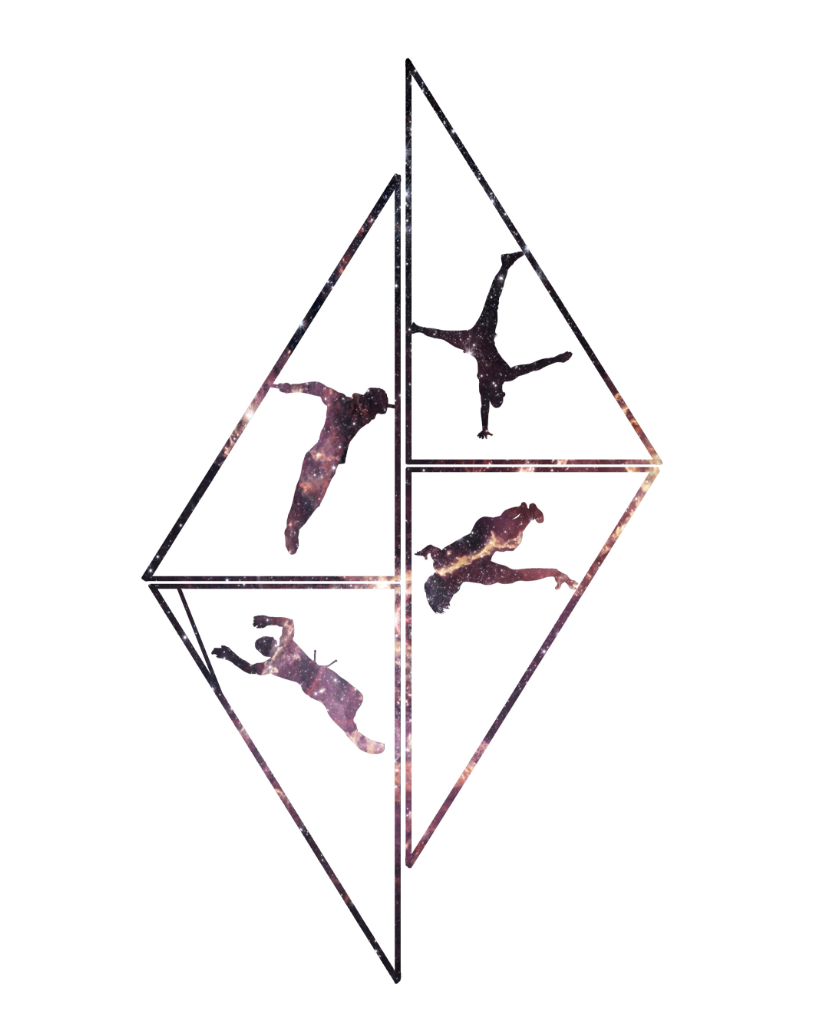
\includegraphics[width=0.4\linewidth]{test.png}\\ \textbf{Street Workout Fusion} \\ \textbf{Regulamin kategorii Freestyle}}
%\author{Grzegorz Jędrzejowski, Dominik Pazdyk, Jan Bajszczak, \\ Maciej Buganik,   Stefan Majkowski, Cezary Dymkowski, \\ Ryszard Kulbaka, Marcin Falenta, Natalia Modzelewska, \\ Karol Siwek, Adrian Gut, Maksym Riznyk}
\author{Jan Bajszczak, Damian Boryga, Maciej Buganik, Michał Drozd, \\ Cezary Dymkowski, Marcin Falenta, Tomasz Grubski, Adrian Gut, \\ Grzegorz Jędrzejowski, Ryszard Kulbaka, Stefan Majkowski, Natalia Modzelewska, \\ Dominik Pazdyk, Krzysztof Piotrowski, Maksym Riznyk, Karol Siwek, Michał Urbanik }

\date{01.09.2023 r. \\ Wersja 1.1}


\begin{document}

  
\maketitle
\newpage

\section*{Postanowienia}
\begin{itemize}
  \item Poniższy regulamin jest objęty prawami autorskimi. Wszelkie prawa zastrzeżone. Bez pisemnej zgody twórców regulamin nie może być tłumaczony na inne języki, publikowany, reprodukowany, powielany ani przetwarzany z~zastosowaniem jakichkolwiek środków elektronicznych, fotokopiarskich, mechanicznych, nagrywających i~innych.
\item Autorzy regulaminu zastrzegają sobie prawo do
wprowadzania zmian do poniższego regulaminu.
\item Wszelkie uwagi oraz sugestie należy złożyć drogą mailową pod adres: streetworkoutfusion@gmail.com.

\end{itemize}
\section*{Podziękowania}
Regulamin został utworzony dzięki kolektywnemu i~bezinteresownemu wysiłkowi jaki włożyła polska społeczność Street Workout. Chcielibyśmy złożyć serdeczne podziękowania dla wszystkich autorów oraz osobom, które wspierały prace na wszystkich jej etapach. W~szczególności podziękowania należą się Krzysztofowi Piotrowskiemu za stworzenie logotypu naszej inicjatywy; Tomaszowi Grubskiemu, który utworzył narzędzie do sprawnej kalkulacji punktów; biernej słuchaczce Natalii Brożynie; Mateuszowi Nowickiemu, Patrykowi Musielakowi, Patrykowi Ziółkowskiemu, Liwii Kalisz i~Antoniemu Sygnatowi za opiniowanie wykonywanych prac oraz Rafałowi Rembalskiemu za zaangażowanie we wczesnych fazach projektu. 
\section*{Wstęp}
Celem twórców jest przyczynienie się do~rozwoju Street Workout-u w~Polsce. Przy tworzeniu poniższego regulaminu skupiono się na aspekcie sprawnego przeprowadzenia wydarzenia, jego widowiskowości oraz obiektywności i~profesjonaliźmie oceny, zapewniając przy tym odpowiednie narzędzia. Bazowano na dokumencie zastosowanym na wydarzeniu Caliathletics Highlander Cup vol. 3 za zgodą autorów. Zebrano grono osób, wśród których znaleźli się organizatorzy, sędziowie oraz aktywni i~byli zawodnicy. Poniższy regulamin powstał do oceny kategorii Freestyle rozumianej jako styl wolny. W~swoich założeniach ma pozwolić na reprezentatywność dużej ilości styli, w~myśli czego ma utworzyć wiele dróg prowadzących do zwycięstwa.  Zasady oceniania zostały tak skonstruowane, aby szczególnie nagradzać zaawansowane kombinacje i~elementy o~wysokim poziomie trudności. W~szczególności poniższy regulamin nie narzuca wymogu kompletności, a~w~zamian skupia się na możliwie najbardziej sprawiedliwej ocenie elementów między kategoriami dynamika akrobatyczna, dynamika siłowa, statyka i~wszystkich ich podpłaszczyzn. Szczególny nacisk kładziony jest na czystość wykonywanych elementów oraz odbiór występu. Niniejszy dokument w~swoim założeniu ma być krokiem w~stronę standaryzacji Street Workout-u. Twórcy zachęcają organizatorów do korzystania z~regulaminu Street Workout Fusion po uprzedniej konsultacji drogą mailową. Powstały regulamin będzie cyklicznie aktualizowany na podstawie informacji zwrotnej społeczności polskiego Street Workout-u.


\newpage
\tableofcontents

\begin{comment}
{\small
\thispagestyle{empty}
\vfill
\begin{center}
Copyright \copyright\; 2023 Street Workout Fusion\\
Wszelkie prawa zastrzeżone\\

ISBN: 978-1-4610-9314-5\\
\textbf{Library of Congress Control Number: 2011905974}
\end{center}}
\end{comment}


\newpage
\section{Aktualizacje}
Poniższa sekcja zawiera w~sobię listę aktualizacji wprowadzonych do ostatniej wersji z~dnia 01.09.2023. Zmiany dla wygody odbiorcy zostały zebrane w~formie listy:
\begin{itemize}
\item W~sekcji \ref{sec:ogolnewyroznienia} dodano wyróżnienia o~premiowaniu pozycji izometrycznej wykonanej po ruchu dynamiki siłowej lub akrobatycznej.
\item W~tabeli \ref{tab:statyka} uzupełniono brakujące wartości punktowe Front Lever SAT Width. Dodano Biceps Close Grip Planche oraz Biceps Biacromial Planche. 
\item Zmieniono wszystkie elementy z~"SAT Width" w~nazwie na "Wide 45 Degrees".
\item Zmieniono kategorie elementu statycznego Iron Cross z~Push na Reverse Pull/Push.
\item Zmieniono definicję Victorian-a w~Tabeli \ref{tab:definicjestata} pozwalając na formę z ugiętymi rękoma powyżej wysokości poręczy. 
\item W~Tabeli \ref{tab:dynamikasilowa} zmieniono Press to Handstand na rozróżnienie wariacji na prostych i~zgiętych rękach. Obniżono punktację: Front Lever Pull Up Wide 45 Degrees, Wide 45 Degrees to Touch; Podniesiono punktację Straight Arm Pull Up oraz Caruso.
\item W~Tabeli \ref{tab:dynamika} zwiększono punktację: Gainer + Half Twist Dismount, Back To Front Dismount, Standing Back Flip Dismount, Standing Front Flip Dismount,
Back To Back Dismount,
Front To Front Dismount,
Giant To Front Flip Dismount,
Gainer + Full Twist Dismount, Standing Front Flip Regrab,
Front Flip Regrab Pronation, Standing Back Flip Regrab, Tornado 360, Dislocated 360, X-Grip 360, Swing 360 Elbow, Swing 360 Front, One Arm Dragon 360, Dragon 540, Swing 540, Dragon 540 To Dislocation, 540 No Touch, Supra 540, Dynamic Pullover, Giant Pronation, Giant 180, Shrimp Flip, Shrimp Flip to Dislocation, Shrimp Flip 360, Geinger, Reverse Geinger, Dislocated Geinger, Freesbie, V-Muscle Up, V-Muscle Up Over the Bar, V-Muscle Up Over the Bar to Supination, Wymyk Ukraiński, Alley Hoop, X-Grip Alley Hoop, Alley Hoop to Dislocation, Palm Spin 180, Palm Spin 360, 180 V-Muscle Up, 180 V-Muscle Up Over the Bar, 180 V-Muscle Up Over the Bar to Supination, Muscle Up 540, Tkachev Regrab Straddle Dislocated,
Front Flip Regrab P-Bars; Obniżono punktację: 
Front Flip Regrab Supra, 
Back Flip Under P-Bars.
\item Doprecyzowanie przerwań ciągłości w~sekcji \ref{sec:ciaglosc}.

  
\end{itemize}
\newpage
\begin{comment}\\ ISBN: \end{comment}


\section{Wymagania ogólne wobec sędziów}
\begin{itemize}
\item Sędziowie muszą być osobami o wysokim morale, nie mogą mieć konfliktu interesów z~jakimkolwiek z~zawodników, muszą być obiektywni;
\item Sędziowie nie mogą brać udziału w występie żadnego z zawodników;
\item Przed zawodami sędziowie muszą zapoznać się z~regulaminem oraz dokładnie znać
zasady oceniania;
\item Sędziowie nie mogą dopingować żadnego z zawodników, jedyną dopuszczalną formą
aplauzu w trakcie występu jest nagrodzenie brawami.
\end{itemize}




\section{Ogólne zasady Oceniania}
\begin{itemize}
\item Regulamin służy do oceny formuły pojedynków oraz występów solowych;
\item W kategorii Freestyle oceniać będzie minimum trzech sędziów:
\begin{enumerate}
\item sędzia elementów dynamiki siłowej,
\item sędzia elementów statycznych,
\item sędzia elementów dynamiki akrobatycznej.
\end{enumerate}
\item W czasie występu, sędziowie będą oceniać wszelkie elementy Street Workout zawarte w~regulamine;
\item Elementy nieznajdujące się w regulaminie powinny zostać wysłane z~przynajmniej tygodniowym wyprzedzeniem (streetworkoutfusion@gmail.com) w~celu ocenienia i~zaakceptowania ich przez skład sędziowski. Mail powinien zawierać nazwę elementu oraz autorskie nagranie prezentujące element, o~którego dodanie ubiega się zawodnik;
\item Elementy z innych sportów, w szczególności: Freerun, Parkour, Pole Dance, Gimbarr, nie będą podlegać punktacji. 
\item Każdy z zawodników może używać magnezji podczas występu;
\item Zawodnicy oceniani będą za elementy wykonywane na sprzęcie udostępnionym przez organizatora.
\item Zawodnicy mogą używać rękawiczek lub stabilizatorów na nadgarstki;
\item Wszelkiego rodzaju sprzęt pomocniczy niewymieniony w regulaminie dozwolony jest tylko po
uprzedniej konsultacji ze składem sędziowskim. Zapytanie należy złożyć do tygodnia przed wydarzeniem drogą mailową (streetworkoutfusion@gmail.com);
\item Zabrania się wykonywania jakichkolwiek obraźliwych, niecenzuralnych gestów oraz zachowań względem sędziów, innych uczestników, organizatora oraz publiczności w
trakcie trwania zawodów. Niedostosowanie się będzie karane dyskwalifikacją
zawodnika;
\item Wyniki punktowe zostaną opublikowane maksymalnie 7 dni od zakończenia zawodów;
\item Wyniki punktowe z poszczególnych rund, oraz wyniki końcowe są niepodważalne i~ostateczne;
\item Zdanie sędziego, jak i przyznana przez niego ilość punktów w trakcie zawodów jest niekwestionowalna;
\item Ubiór zawodnika nie może zaburzać oceny elementów;
\item Zawodnicy mogą startować bez butów;
\item Zawodnik może przerwać występ przed ukończeniem czasu, sygnalizując to w~jednoznaczny sposób, np. krzyżując ręce na wysokości głowy.
\end{itemize}


\section{Ocenianie elementów statycznych}
\begin{itemize}
\item Elementy statyczne oceniane są przez sędziego, któremu podlega podana kategoria. Sędzia dokonuje oceny na podstawie bazowej punktacji poziomu trudności elementów statycznych;
\item Sędzia przydziela kary opisane w~sekcji \ref{sec:systemkar} oraz bonusy opisane w~sekcji \ref{sec:systempremiowania} zgodnie z~definicjami \ref{tab:definicjestata};
\item  Każda figura statyczna musi zostać przytrzymana 2 sekundy. Czas przytrzymania pozycji rozumie się jako czas od momentu wejścia i~zatrzymania pozycji docelowej. Wchodzenie do pozycji i~opadanie nie jest liczone jako czas przytrzymania. Elementy poniżej 2 sekund nie będą zaliczane;

\item Za figurę przytrzymaną uważa się pozycję izometryczną, bez ruchu;

\item Elementy są punktowane według tabel \ref{tab:statyka}, \ref{tab:statykak};
\item Uzyskanie najwyższej możliwej liczby punktów za wykonanie elementu wymaga perfekcyjnej techniki;
\end{itemize}
\subsection{Tabela punktowa elementów statycznych mężczyzn}
%mężczyzn

    \begin{longtable}{|lccccccccc|}
      \caption{Wartości punktowe elementów statycznych mężczyzn. Skróty oznaczają: PB - poręcze, DS - drążek supinacja, DP - drążek pronacja, ZS - ziemia supinacja, ZP - ziemia pronacja, KS - koła supinacja, KP - koła pronacja, V - pionowe drążki.}
      \label{tab:statyka}
      \endfirsthead
      \endhead


      \hline
\rowcolor[HTML]{34A853} 
\multicolumn{10}{|c|}{\cellcolor[HTML]{34A853}\textbf{STATYKA MĘŻCZYZN}}                                                                                                                                                                                                                                                                                                                                                                                                                                                                                                                                                   \\ \hline
\rowcolor[HTML]{B6D7A8} 
\multicolumn{10}{|c|}{\cellcolor[HTML]{B6D7A8}\textbf{PLANCHE}}                                                                                                                                                                                                                                                                                                                                                                                                                                                                                                                                                            \\ \hline
\rowcolor[HTML]{CCCCCC} 
\multicolumn{1}{|c|}{\cellcolor[HTML]{CCCCCC}\textbf{ELEMENT}}                      & \multicolumn{1}{c|}{\cellcolor[HTML]{CCCCCC}\textbf{Kategoria}} & \multicolumn{1}{c|}{\cellcolor[HTML]{CCCCCC}\textbf{PB}}  & \multicolumn{1}{c|}{\cellcolor[HTML]{CCCCCC}\textbf{DS}}  & \multicolumn{1}{c|}{\cellcolor[HTML]{CCCCCC}\textbf{DP}} & \multicolumn{1}{c|}{\cellcolor[HTML]{CCCCCC}\textbf{ZS}} & \multicolumn{1}{c|}{\cellcolor[HTML]{CCCCCC}\textbf{ZP}} & \multicolumn{1}{c|}{\cellcolor[HTML]{CCCCCC}\textbf{KS}} & \multicolumn{1}{c|}{\cellcolor[HTML]{CCCCCC}\textbf{KP}}  & \textbf{V}                         \\ \hline
\multicolumn{1}{|l|}{\cellcolor[HTML]{FFFFFF}\textbf{BIACROMIAL}}                   & \multicolumn{1}{c|}{\textbf{P}}                                 & \multicolumn{1}{c|}{\cellcolor[HTML]{FFFFFF}\textbf{10}}  & \multicolumn{1}{c|}{\cellcolor[HTML]{FFFFFF}\textbf{15}}  & \multicolumn{1}{c|}{\cellcolor[HTML]{FFFFFF}\textbf{13}} & \multicolumn{1}{c|}{\cellcolor[HTML]{FFFFFF}\textbf{20}} & \multicolumn{1}{c|}{\cellcolor[HTML]{FFFFFF}\textbf{12}} & \multicolumn{1}{c|}{\cellcolor[HTML]{FFFFFF}\textbf{25}} & \multicolumn{1}{c|}{\cellcolor[HTML]{FFFFFF}\textbf{-}}   & \cellcolor[HTML]{FFFFFF}\textbf{-} \\ \hline
\rowcolor[HTML]{EFEFEF} 
\multicolumn{1}{|l|}{\cellcolor[HTML]{EFEFEF}\textbf{STRADDLE}}                     & \multicolumn{1}{c|}{\cellcolor[HTML]{EFEFEF}\textbf{P}}         & \multicolumn{1}{c|}{\cellcolor[HTML]{EFEFEF}\textbf{6}}   & \multicolumn{1}{c|}{\cellcolor[HTML]{EFEFEF}\textbf{9}}   & \multicolumn{1}{c|}{\cellcolor[HTML]{EFEFEF}\textbf{8}}  & \multicolumn{1}{c|}{\cellcolor[HTML]{EFEFEF}\textbf{12}} & \multicolumn{1}{c|}{\cellcolor[HTML]{EFEFEF}\textbf{7}}  & \multicolumn{1}{c|}{\cellcolor[HTML]{EFEFEF}\textbf{15}} & \multicolumn{1}{c|}{\cellcolor[HTML]{EFEFEF}\textbf{-}}   & \textbf{-}                         \\ \hline
\multicolumn{1}{|l|}{\cellcolor[HTML]{FFFFFF}\textbf{WIDE 45 DEGREES}}              & \multicolumn{1}{c|}{\textbf{P}}                                 & \multicolumn{1}{c|}{\cellcolor[HTML]{FFFFFF}\textbf{14}}  & \multicolumn{1}{c|}{\cellcolor[HTML]{FFFFFF}\textbf{20}}  & \multicolumn{1}{c|}{\cellcolor[HTML]{FFFFFF}\textbf{16}} & \multicolumn{1}{c|}{\cellcolor[HTML]{FFFFFF}\textbf{27}} & \multicolumn{1}{c|}{\cellcolor[HTML]{FFFFFF}\textbf{16}} & \multicolumn{1}{c|}{\cellcolor[HTML]{FFFFFF}\textbf{34}} & \multicolumn{1}{c|}{\cellcolor[HTML]{FFFFFF}\textbf{-}}   & \cellcolor[HTML]{FFFFFF}\textbf{-} \\ \hline
\rowcolor[HTML]{EFEFEF} 
\multicolumn{1}{|l|}{\cellcolor[HTML]{EFEFEF}\textbf{STRADDLE}}                     & \multicolumn{1}{c|}{\cellcolor[HTML]{EFEFEF}\textbf{P}}         & \multicolumn{1}{c|}{\cellcolor[HTML]{EFEFEF}\textbf{8}}   & \multicolumn{1}{c|}{\cellcolor[HTML]{EFEFEF}\textbf{12}}  & \multicolumn{1}{c|}{\cellcolor[HTML]{EFEFEF}\textbf{10}} & \multicolumn{1}{c|}{\cellcolor[HTML]{EFEFEF}\textbf{16}} & \multicolumn{1}{c|}{\cellcolor[HTML]{EFEFEF}\textbf{10}} & \multicolumn{1}{c|}{\cellcolor[HTML]{EFEFEF}\textbf{20}} & \multicolumn{1}{c|}{\cellcolor[HTML]{EFEFEF}\textbf{-}}   & \textbf{-}                         \\ \hline
\multicolumn{1}{|l|}{\cellcolor[HTML]{FFFFFF}\textbf{CLOSE GRIP}}                   & \multicolumn{1}{c|}{\textbf{P}}                                 & \multicolumn{1}{c|}{\cellcolor[HTML]{FFFFFF}\textbf{-}}   & \multicolumn{1}{c|}{\cellcolor[HTML]{FFFFFF}\textbf{19}}  & \multicolumn{1}{c|}{\cellcolor[HTML]{FFFFFF}\textbf{20}} & \multicolumn{1}{c|}{\cellcolor[HTML]{FFFFFF}\textbf{-}}  & \multicolumn{1}{c|}{\cellcolor[HTML]{FFFFFF}\textbf{16}} & \multicolumn{1}{c|}{\cellcolor[HTML]{FFFFFF}\textbf{-}}  & \multicolumn{1}{c|}{\cellcolor[HTML]{FFFFFF}\textbf{-}}   & \cellcolor[HTML]{FFFFFF}\textbf{-} \\ \hline
\rowcolor[HTML]{EFEFEF} 
\multicolumn{1}{|l|}{\cellcolor[HTML]{EFEFEF}\textbf{STRADDLE}}                     & \multicolumn{1}{c|}{\cellcolor[HTML]{EFEFEF}\textbf{P}}         & \multicolumn{1}{c|}{\cellcolor[HTML]{EFEFEF}\textbf{-}}   & \multicolumn{1}{c|}{\cellcolor[HTML]{EFEFEF}\textbf{12}}  & \multicolumn{1}{c|}{\cellcolor[HTML]{EFEFEF}\textbf{10}} & \multicolumn{1}{c|}{\cellcolor[HTML]{EFEFEF}\textbf{-}}  & \multicolumn{1}{c|}{\cellcolor[HTML]{EFEFEF}\textbf{10}} & \multicolumn{1}{c|}{\cellcolor[HTML]{EFEFEF}\textbf{-}}  & \multicolumn{1}{c|}{\cellcolor[HTML]{EFEFEF}\textbf{-}}   & \textbf{-}                         \\ \hline
\multicolumn{1}{|l|}{\cellcolor[HTML]{FFFFFF}\textbf{IGUANA}}                       & \multicolumn{1}{c|}{\textbf{P}}                                 & \multicolumn{1}{c|}{\cellcolor[HTML]{FFFFFF}\textbf{25}}  & \multicolumn{1}{c|}{\cellcolor[HTML]{FFFFFF}\textbf{-}}   & \multicolumn{1}{c|}{\cellcolor[HTML]{FFFFFF}\textbf{-}}  & \multicolumn{1}{c|}{\cellcolor[HTML]{FFFFFF}\textbf{-}}  & \multicolumn{1}{c|}{\cellcolor[HTML]{FFFFFF}\textbf{-}}  & \multicolumn{1}{c|}{\cellcolor[HTML]{FFFFFF}\textbf{-}}  & \multicolumn{1}{c|}{\cellcolor[HTML]{FFFFFF}\textbf{-}}   & \cellcolor[HTML]{FFFFFF}\textbf{-} \\ \hline
\rowcolor[HTML]{EFEFEF} 
\multicolumn{1}{|l|}{\cellcolor[HTML]{EFEFEF}\textbf{STRADDLE}}                     & \multicolumn{1}{c|}{\cellcolor[HTML]{EFEFEF}\textbf{P}}         & \multicolumn{1}{c|}{\cellcolor[HTML]{EFEFEF}\textbf{18}}  & \multicolumn{1}{c|}{\cellcolor[HTML]{EFEFEF}\textbf{-}}   & \multicolumn{1}{c|}{\cellcolor[HTML]{EFEFEF}\textbf{-}}  & \multicolumn{1}{c|}{\cellcolor[HTML]{EFEFEF}\textbf{-}}  & \multicolumn{1}{c|}{\cellcolor[HTML]{EFEFEF}\textbf{-}}  & \multicolumn{1}{c|}{\cellcolor[HTML]{EFEFEF}\textbf{-}}  & \multicolumn{1}{c|}{\cellcolor[HTML]{EFEFEF}\textbf{-}}   & \textbf{-}                         \\ \hline
\multicolumn{1}{|l|}{\cellcolor[HTML]{FFFFFF}\textbf{DEAD}}                         & \multicolumn{1}{c|}{\textbf{P}}                                 & \multicolumn{1}{c|}{\cellcolor[HTML]{FFFFFF}\textbf{12}}  & \multicolumn{1}{c|}{\cellcolor[HTML]{FFFFFF}\textbf{-}}   & \multicolumn{1}{c|}{\cellcolor[HTML]{FFFFFF}\textbf{-}}  & \multicolumn{1}{c|}{\cellcolor[HTML]{FFFFFF}\textbf{-}}  & \multicolumn{1}{c|}{\cellcolor[HTML]{FFFFFF}\textbf{-}}  & \multicolumn{1}{c|}{\cellcolor[HTML]{FFFFFF}\textbf{-}}  & \multicolumn{1}{c|}{\cellcolor[HTML]{FFFFFF}\textbf{-}}   & \cellcolor[HTML]{FFFFFF}\textbf{-} \\ \hline
\rowcolor[HTML]{EFEFEF} 
\multicolumn{1}{|l|}{\cellcolor[HTML]{EFEFEF}\textbf{STRADDLE}}                     & \multicolumn{1}{c|}{\cellcolor[HTML]{EFEFEF}\textbf{P}}         & \multicolumn{1}{c|}{\cellcolor[HTML]{EFEFEF}\textbf{7}}   & \multicolumn{1}{c|}{\cellcolor[HTML]{EFEFEF}\textbf{-}}   & \multicolumn{1}{c|}{\cellcolor[HTML]{EFEFEF}\textbf{-}}  & \multicolumn{1}{c|}{\cellcolor[HTML]{EFEFEF}\textbf{-}}  & \multicolumn{1}{c|}{\cellcolor[HTML]{EFEFEF}\textbf{-}}  & \multicolumn{1}{c|}{\cellcolor[HTML]{EFEFEF}\textbf{-}}  & \multicolumn{1}{c|}{\cellcolor[HTML]{EFEFEF}\textbf{-}}   & \textbf{-}                         \\ \hline
\multicolumn{1}{|l|}{\cellcolor[HTML]{FFFFFF}\textbf{BICEPS CLOSE GRIP}}            & \multicolumn{1}{c|}{\textbf{P}}                                 & \multicolumn{1}{c|}{\cellcolor[HTML]{FFFFFF}\textbf{13}}  & \multicolumn{1}{c|}{\cellcolor[HTML]{FFFFFF}\textbf{-}}   & \multicolumn{1}{c|}{\cellcolor[HTML]{FFFFFF}\textbf{-}}  & \multicolumn{1}{c|}{\cellcolor[HTML]{FFFFFF}\textbf{-}}  & \multicolumn{1}{c|}{\cellcolor[HTML]{FFFFFF}\textbf{-}}  & \multicolumn{1}{c|}{\cellcolor[HTML]{FFFFFF}\textbf{-}}  & \multicolumn{1}{c|}{\cellcolor[HTML]{FFFFFF}\textbf{-}}   & \cellcolor[HTML]{FFFFFF}\textbf{-} \\ \hline
\rowcolor[HTML]{EFEFEF} 
\multicolumn{1}{|l|}{\cellcolor[HTML]{EFEFEF}\textbf{STRADDLE}}                     & \multicolumn{1}{c|}{\cellcolor[HTML]{EFEFEF}\textbf{P}}         & \multicolumn{1}{c|}{\cellcolor[HTML]{EFEFEF}\textbf{8}}   & \multicolumn{1}{c|}{\cellcolor[HTML]{EFEFEF}\textbf{-}}   & \multicolumn{1}{c|}{\cellcolor[HTML]{EFEFEF}\textbf{-}}  & \multicolumn{1}{c|}{\cellcolor[HTML]{EFEFEF}\textbf{-}}  & \multicolumn{1}{c|}{\cellcolor[HTML]{EFEFEF}\textbf{-}}  & \multicolumn{1}{c|}{\cellcolor[HTML]{EFEFEF}\textbf{-}}  & \multicolumn{1}{c|}{\cellcolor[HTML]{EFEFEF}\textbf{-}}   & \textbf{-}                         \\ \hline
\multicolumn{1}{|l|}{\cellcolor[HTML]{FFFFFF}\textbf{BICEPS BIACROMIAL}}            & \multicolumn{1}{c|}{\textbf{P}}                                 & \multicolumn{1}{c|}{\cellcolor[HTML]{FFFFFF}\textbf{14}}  & \multicolumn{1}{c|}{\cellcolor[HTML]{FFFFFF}\textbf{-}}   & \multicolumn{1}{c|}{\cellcolor[HTML]{FFFFFF}\textbf{-}}  & \multicolumn{1}{c|}{\cellcolor[HTML]{FFFFFF}\textbf{-}}  & \multicolumn{1}{c|}{\cellcolor[HTML]{FFFFFF}\textbf{-}}  & \multicolumn{1}{c|}{\cellcolor[HTML]{FFFFFF}\textbf{-}}  & \multicolumn{1}{c|}{\cellcolor[HTML]{FFFFFF}\textbf{-}}   & \cellcolor[HTML]{FFFFFF}\textbf{-} \\ \hline
\rowcolor[HTML]{EFEFEF} 
\multicolumn{1}{|l|}{\cellcolor[HTML]{EFEFEF}\textbf{STRADDLE}}                     & \multicolumn{1}{c|}{\cellcolor[HTML]{EFEFEF}\textbf{P}}         & \multicolumn{1}{c|}{\cellcolor[HTML]{EFEFEF}\textbf{9}}   & \multicolumn{1}{c|}{\cellcolor[HTML]{EFEFEF}\textbf{-}}   & \multicolumn{1}{c|}{\cellcolor[HTML]{EFEFEF}\textbf{-}}  & \multicolumn{1}{c|}{\cellcolor[HTML]{EFEFEF}\textbf{-}}  & \multicolumn{1}{c|}{\cellcolor[HTML]{EFEFEF}\textbf{-}}  & \multicolumn{1}{c|}{\cellcolor[HTML]{EFEFEF}\textbf{-}}  & \multicolumn{1}{c|}{\cellcolor[HTML]{EFEFEF}\textbf{-}}   & \textbf{-}                         \\ \hline
\multicolumn{1}{|l|}{\cellcolor[HTML]{FFFFFF}\textbf{PRAYER}}                       & \multicolumn{1}{c|}{\textbf{P}}                                 & \multicolumn{1}{c|}{\cellcolor[HTML]{FFFFFF}\textbf{-}}   & \multicolumn{1}{c|}{\cellcolor[HTML]{FFFFFF}\textbf{-}}   & \multicolumn{1}{c|}{\cellcolor[HTML]{FFFFFF}\textbf{-}}  & \multicolumn{1}{c|}{\cellcolor[HTML]{FFFFFF}\textbf{-}}  & \multicolumn{1}{c|}{\cellcolor[HTML]{FFFFFF}\textbf{12}} & \multicolumn{1}{c|}{\cellcolor[HTML]{FFFFFF}\textbf{-}}  & \multicolumn{1}{c|}{\cellcolor[HTML]{FFFFFF}\textbf{-}}   & \cellcolor[HTML]{FFFFFF}\textbf{-} \\ \hline
\rowcolor[HTML]{EFEFEF} 
\multicolumn{1}{|l|}{\cellcolor[HTML]{EFEFEF}\textbf{STRADDLE}}                     & \multicolumn{1}{c|}{\cellcolor[HTML]{EFEFEF}\textbf{P}}         & \multicolumn{1}{c|}{\cellcolor[HTML]{EFEFEF}\textbf{-}}   & \multicolumn{1}{c|}{\cellcolor[HTML]{EFEFEF}\textbf{-}}   & \multicolumn{1}{c|}{\cellcolor[HTML]{EFEFEF}\textbf{-}}  & \multicolumn{1}{c|}{\cellcolor[HTML]{EFEFEF}\textbf{-}}  & \multicolumn{1}{c|}{\cellcolor[HTML]{EFEFEF}\textbf{7}}  & \multicolumn{1}{c|}{\cellcolor[HTML]{EFEFEF}\textbf{-}}  & \multicolumn{1}{c|}{\cellcolor[HTML]{EFEFEF}\textbf{-}}   & \textbf{-}                         \\ \hline
\multicolumn{1}{|l|}{\cellcolor[HTML]{FFFFFF}\textbf{REVERSE GRIP}}                 & \multicolumn{1}{c|}{\textbf{P}}                                 & \multicolumn{1}{c|}{\cellcolor[HTML]{FFFFFF}\textbf{-}}   & \multicolumn{1}{c|}{\cellcolor[HTML]{FFFFFF}\textbf{-}}   & \multicolumn{1}{c|}{\cellcolor[HTML]{FFFFFF}\textbf{-}}  & \multicolumn{1}{c|}{\cellcolor[HTML]{FFFFFF}\textbf{-}}  & \multicolumn{1}{c|}{\cellcolor[HTML]{FFFFFF}\textbf{16}} & \multicolumn{1}{c|}{\cellcolor[HTML]{FFFFFF}\textbf{-}}  & \multicolumn{1}{c|}{\cellcolor[HTML]{FFFFFF}\textbf{-}}   & \cellcolor[HTML]{FFFFFF}\textbf{-} \\ \hline
\rowcolor[HTML]{EFEFEF} 
\multicolumn{1}{|l|}{\cellcolor[HTML]{EFEFEF}\textbf{STRADDLE}}                     & \multicolumn{1}{c|}{\cellcolor[HTML]{EFEFEF}\textbf{P}}         & \multicolumn{1}{c|}{\cellcolor[HTML]{EFEFEF}\textbf{-}}   & \multicolumn{1}{c|}{\cellcolor[HTML]{EFEFEF}\textbf{-}}   & \multicolumn{1}{c|}{\cellcolor[HTML]{EFEFEF}\textbf{-}}  & \multicolumn{1}{c|}{\cellcolor[HTML]{EFEFEF}\textbf{-}}  & \multicolumn{1}{c|}{\cellcolor[HTML]{EFEFEF}\textbf{9}}  & \multicolumn{1}{c|}{\cellcolor[HTML]{EFEFEF}\textbf{-}}  & \multicolumn{1}{c|}{\cellcolor[HTML]{EFEFEF}\textbf{-}}   & \textbf{-}                         \\ \hline
\multicolumn{1}{|l|}{\cellcolor[HTML]{FFFFFF}\textbf{REVERSE CLOSE GRIP}}           & \multicolumn{1}{c|}{\textbf{P}}                                 & \multicolumn{1}{c|}{\cellcolor[HTML]{FFFFFF}\textbf{-}}   & \multicolumn{1}{c|}{\cellcolor[HTML]{FFFFFF}\textbf{-}}   & \multicolumn{1}{c|}{\cellcolor[HTML]{FFFFFF}\textbf{-}}  & \multicolumn{1}{c|}{\cellcolor[HTML]{FFFFFF}\textbf{-}}  & \multicolumn{1}{c|}{\cellcolor[HTML]{FFFFFF}\textbf{20}} & \multicolumn{1}{c|}{\cellcolor[HTML]{FFFFFF}\textbf{-}}  & \multicolumn{1}{c|}{\cellcolor[HTML]{FFFFFF}\textbf{-}}   & \cellcolor[HTML]{FFFFFF}\textbf{-} \\ \hline
\rowcolor[HTML]{EFEFEF} 
\multicolumn{1}{|l|}{\cellcolor[HTML]{EFEFEF}\textbf{STRADDLE}}                     & \multicolumn{1}{c|}{\cellcolor[HTML]{EFEFEF}\textbf{P}}         & \multicolumn{1}{c|}{\cellcolor[HTML]{EFEFEF}\textbf{-}}   & \multicolumn{1}{c|}{\cellcolor[HTML]{EFEFEF}\textbf{-}}   & \multicolumn{1}{c|}{\cellcolor[HTML]{EFEFEF}\textbf{-}}  & \multicolumn{1}{c|}{\cellcolor[HTML]{EFEFEF}\textbf{-}}  & \multicolumn{1}{c|}{\cellcolor[HTML]{EFEFEF}\textbf{12}} & \multicolumn{1}{c|}{\cellcolor[HTML]{EFEFEF}\textbf{-}}  & \multicolumn{1}{c|}{\cellcolor[HTML]{EFEFEF}\textbf{-}}   & \textbf{-}                         \\ \hline
\multicolumn{1}{|l|}{\cellcolor[HTML]{FFFFFF}\textbf{SIDE}}                         & \multicolumn{1}{c|}{\textbf{P}}                                 & \multicolumn{1}{c|}{\cellcolor[HTML]{FFFFFF}\textbf{8}}   & \multicolumn{1}{c|}{\cellcolor[HTML]{FFFFFF}\textbf{9}}   & \multicolumn{1}{c|}{\cellcolor[HTML]{FFFFFF}\textbf{8}}  & \multicolumn{1}{c|}{\cellcolor[HTML]{FFFFFF}\textbf{10}} & \multicolumn{1}{c|}{\cellcolor[HTML]{FFFFFF}\textbf{8}}  & \multicolumn{1}{c|}{\cellcolor[HTML]{FFFFFF}\textbf{-}}  & \multicolumn{1}{c|}{\cellcolor[HTML]{FFFFFF}\textbf{-}}   & \cellcolor[HTML]{FFFFFF}\textbf{-} \\ \hline
\rowcolor[HTML]{EFEFEF} 
\multicolumn{1}{|l|}{\cellcolor[HTML]{EFEFEF}\textbf{STRADDLE}}                     & \multicolumn{1}{c|}{\cellcolor[HTML]{EFEFEF}\textbf{P}}         & \multicolumn{1}{c|}{\cellcolor[HTML]{EFEFEF}\textbf{5}}   & \multicolumn{1}{c|}{\cellcolor[HTML]{EFEFEF}\textbf{6}}   & \multicolumn{1}{c|}{\cellcolor[HTML]{EFEFEF}\textbf{5}}  & \multicolumn{1}{c|}{\cellcolor[HTML]{EFEFEF}\textbf{6}}  & \multicolumn{1}{c|}{\cellcolor[HTML]{EFEFEF}\textbf{5}}  & \multicolumn{1}{c|}{\cellcolor[HTML]{EFEFEF}\textbf{-}}  & \multicolumn{1}{c|}{\cellcolor[HTML]{EFEFEF}\textbf{-}}   & \textbf{-}                         \\ \hline
\multicolumn{1}{|l|}{\cellcolor[HTML]{FFFFFF}\textbf{5 FINGER}}                     & \multicolumn{1}{c|}{\textbf{P}}                                 & \multicolumn{1}{c|}{\cellcolor[HTML]{FFFFFF}\textbf{-}}   & \multicolumn{1}{c|}{\cellcolor[HTML]{FFFFFF}\textbf{-}}   & \multicolumn{1}{c|}{\cellcolor[HTML]{FFFFFF}\textbf{-}}  & \multicolumn{1}{c|}{\cellcolor[HTML]{FFFFFF}\textbf{18}} & \multicolumn{1}{c|}{\cellcolor[HTML]{FFFFFF}\textbf{14}} & \multicolumn{1}{c|}{\cellcolor[HTML]{FFFFFF}\textbf{-}}  & \multicolumn{1}{c|}{\cellcolor[HTML]{FFFFFF}\textbf{-}}   & \cellcolor[HTML]{FFFFFF}\textbf{-} \\ \hline
\rowcolor[HTML]{EFEFEF} 
\multicolumn{1}{|l|}{\cellcolor[HTML]{EFEFEF}\textbf{STRADDLE}}                     & \multicolumn{1}{c|}{\cellcolor[HTML]{EFEFEF}\textbf{P}}         & \multicolumn{1}{c|}{\cellcolor[HTML]{EFEFEF}\textbf{-}}   & \multicolumn{1}{c|}{\cellcolor[HTML]{EFEFEF}\textbf{-}}   & \multicolumn{1}{c|}{\cellcolor[HTML]{EFEFEF}\textbf{-}}  & \multicolumn{1}{c|}{\cellcolor[HTML]{EFEFEF}\textbf{11}} & \multicolumn{1}{c|}{\cellcolor[HTML]{EFEFEF}\textbf{9}}  & \multicolumn{1}{c|}{\cellcolor[HTML]{EFEFEF}\textbf{-}}  & \multicolumn{1}{c|}{\cellcolor[HTML]{EFEFEF}\textbf{-}}   & \textbf{-}                         \\ \hline
\multicolumn{1}{|l|}{\cellcolor[HTML]{FFFFFF}\textbf{2 FINGER}}                     & \multicolumn{1}{c|}{\textbf{P}}                                 & \multicolumn{1}{c|}{\cellcolor[HTML]{FFFFFF}\textbf{35}}  & \multicolumn{1}{c|}{\cellcolor[HTML]{FFFFFF}\textbf{-}}   & \multicolumn{1}{c|}{\cellcolor[HTML]{FFFFFF}\textbf{-}}  & \multicolumn{1}{c|}{\cellcolor[HTML]{FFFFFF}\textbf{-}}  & \multicolumn{1}{c|}{\cellcolor[HTML]{FFFFFF}\textbf{30}} & \multicolumn{1}{c|}{\cellcolor[HTML]{FFFFFF}\textbf{-}}  & \multicolumn{1}{c|}{\cellcolor[HTML]{FFFFFF}\textbf{-}}   & \cellcolor[HTML]{FFFFFF}\textbf{-} \\ \hline
\rowcolor[HTML]{EFEFEF} 
\multicolumn{1}{|l|}{\cellcolor[HTML]{EFEFEF}\textbf{STRADDLE}}                     & \multicolumn{1}{c|}{\cellcolor[HTML]{EFEFEF}\textbf{P}}         & \multicolumn{1}{c|}{\cellcolor[HTML]{EFEFEF}\textbf{21}}  & \multicolumn{1}{c|}{\cellcolor[HTML]{EFEFEF}\textbf{-}}   & \multicolumn{1}{c|}{\cellcolor[HTML]{EFEFEF}\textbf{-}}  & \multicolumn{1}{c|}{\cellcolor[HTML]{EFEFEF}\textbf{-}}  & \multicolumn{1}{c|}{\cellcolor[HTML]{EFEFEF}\textbf{18}} & \multicolumn{1}{c|}{\cellcolor[HTML]{EFEFEF}\textbf{-}}  & \multicolumn{1}{c|}{\cellcolor[HTML]{EFEFEF}\textbf{-}}   & \textbf{-}                         \\ \hline
\multicolumn{1}{|l|}{\cellcolor[HTML]{FFFFFF}\textbf{DRAGON}}                       & \multicolumn{1}{c|}{\textbf{P}}                                 & \multicolumn{1}{c|}{\cellcolor[HTML]{FFFFFF}\textbf{16}}  & \multicolumn{1}{c|}{\cellcolor[HTML]{FFFFFF}\textbf{-}}   & \multicolumn{1}{c|}{\cellcolor[HTML]{FFFFFF}\textbf{-}}  & \multicolumn{1}{c|}{\cellcolor[HTML]{FFFFFF}\textbf{-}}  & \multicolumn{1}{c|}{\cellcolor[HTML]{FFFFFF}\textbf{-}}  & \multicolumn{1}{c|}{\cellcolor[HTML]{FFFFFF}\textbf{-}}  & \multicolumn{1}{c|}{\cellcolor[HTML]{FFFFFF}\textbf{-}}   & \cellcolor[HTML]{FFFFFF}\textbf{-} \\ \hline
\rowcolor[HTML]{EFEFEF} 
\multicolumn{1}{|l|}{\cellcolor[HTML]{EFEFEF}\textbf{STRADDLE}}                     & \multicolumn{1}{c|}{\cellcolor[HTML]{EFEFEF}\textbf{P}}         & \multicolumn{1}{c|}{\cellcolor[HTML]{EFEFEF}\textbf{10}}  & \multicolumn{1}{c|}{\cellcolor[HTML]{EFEFEF}\textbf{-}}   & \multicolumn{1}{c|}{\cellcolor[HTML]{EFEFEF}\textbf{-}}  & \multicolumn{1}{c|}{\cellcolor[HTML]{EFEFEF}\textbf{-}}  & \multicolumn{1}{c|}{\cellcolor[HTML]{EFEFEF}\textbf{-}}  & \multicolumn{1}{c|}{\cellcolor[HTML]{EFEFEF}\textbf{-}}  & \multicolumn{1}{c|}{\cellcolor[HTML]{EFEFEF}\textbf{-}}   & \textbf{-}                         \\ \hline
\rowcolor[HTML]{D5A6BD} 
\multicolumn{10}{|c|}{\cellcolor[HTML]{D5A6BD}\textbf{HANDSTAND}}                                                                                                                                                                                                                                                                                                                                                                                                                                                                                                                                                          \\ \hline
\rowcolor[HTML]{CCCCCC} 
\multicolumn{1}{|c|}{\cellcolor[HTML]{CCCCCC}\textbf{ELEMENT}}                      & \multicolumn{1}{c|}{\cellcolor[HTML]{CCCCCC}\textbf{Kategoria}} & \multicolumn{1}{c|}{\cellcolor[HTML]{CCCCCC}\textbf{PB}}  & \multicolumn{1}{c|}{\cellcolor[HTML]{CCCCCC}\textbf{DS}}  & \multicolumn{1}{c|}{\cellcolor[HTML]{CCCCCC}\textbf{DP}} & \multicolumn{1}{c|}{\cellcolor[HTML]{CCCCCC}\textbf{ZS}} & \multicolumn{1}{c|}{\cellcolor[HTML]{CCCCCC}\textbf{ZP}} & \multicolumn{1}{c|}{\cellcolor[HTML]{CCCCCC}\textbf{KS}} & \multicolumn{1}{c|}{\cellcolor[HTML]{CCCCCC}\textbf{KP}}  & \textbf{V}                         \\ \hline
\multicolumn{1}{|l|}{\cellcolor[HTML]{FFFFFF}\textbf{BIACROMIAL}}                   & \multicolumn{1}{c|}{\textbf{B}}                                 & \multicolumn{1}{c|}{\textbf{2}}                           & \multicolumn{1}{c|}{\textbf{5}}                           & \multicolumn{1}{c|}{\textbf{5}}                          & \multicolumn{1}{c|}{\textbf{7}}                          & \multicolumn{1}{c|}{\textbf{2}}                          & \multicolumn{1}{c|}{\textbf{-}}                          & \multicolumn{1}{c|}{\textbf{12}}                          & \textbf{-}                         \\ \hline
\rowcolor[HTML]{EFEFEF} 
\multicolumn{1}{|l|}{\cellcolor[HTML]{EFEFEF}\textbf{STRADDLE}}                     & \multicolumn{1}{c|}{\cellcolor[HTML]{EFEFEF}\textbf{B}}         & \multicolumn{1}{c|}{\cellcolor[HTML]{EFEFEF}\textbf{1}}   & \multicolumn{1}{c|}{\cellcolor[HTML]{EFEFEF}\textbf{2}}   & \multicolumn{1}{c|}{\cellcolor[HTML]{EFEFEF}\textbf{2}}  & \multicolumn{1}{c|}{\cellcolor[HTML]{EFEFEF}\textbf{3}}  & \multicolumn{1}{c|}{\cellcolor[HTML]{EFEFEF}\textbf{1}}  & \multicolumn{1}{c|}{\cellcolor[HTML]{EFEFEF}\textbf{-}}  & \multicolumn{1}{c|}{\cellcolor[HTML]{EFEFEF}\textbf{-}}   & \textbf{-}                         \\ \hline
\multicolumn{1}{|l|}{\cellcolor[HTML]{FFFFFF}\textbf{WIDE}}                         & \multicolumn{1}{c|}{\textbf{B}}                                 & \multicolumn{1}{c|}{\textbf{4}}                           & \multicolumn{1}{c|}{\textbf{8}}                           & \multicolumn{1}{c|}{\textbf{8}}                          & \multicolumn{1}{c|}{\textbf{10}}                         & \multicolumn{1}{c|}{\textbf{5}}                          & \multicolumn{1}{c|}{\textbf{-}}                          & \multicolumn{1}{c|}{\textbf{-}}                           & \textbf{-}                         \\ \hline
\rowcolor[HTML]{EFEFEF} 
\multicolumn{1}{|l|}{\cellcolor[HTML]{EFEFEF}\textbf{STRADDLE}}                     & \multicolumn{1}{c|}{\cellcolor[HTML]{EFEFEF}\textbf{B}}         & \multicolumn{1}{c|}{\cellcolor[HTML]{EFEFEF}\textbf{2}}   & \multicolumn{1}{c|}{\cellcolor[HTML]{EFEFEF}\textbf{4}}   & \multicolumn{1}{c|}{\cellcolor[HTML]{EFEFEF}\textbf{4}}  & \multicolumn{1}{c|}{\cellcolor[HTML]{EFEFEF}\textbf{5}}  & \multicolumn{1}{c|}{\cellcolor[HTML]{EFEFEF}\textbf{2}}  & \multicolumn{1}{c|}{\cellcolor[HTML]{EFEFEF}\textbf{-}}  & \multicolumn{1}{c|}{\cellcolor[HTML]{EFEFEF}\textbf{-}}   & \textbf{-}                         \\ \hline
\multicolumn{1}{|l|}{\textbf{CLOSE GRIP}}                                           & \multicolumn{1}{c|}{\textbf{B}}                                 & \multicolumn{1}{c|}{\textbf{2}}                           & \multicolumn{1}{c|}{\textbf{8}}                           & \multicolumn{1}{c|}{\textbf{7}}                          & \multicolumn{1}{c|}{\textbf{9}}                          & \multicolumn{1}{c|}{\textbf{4}}                          & \multicolumn{1}{c|}{\textbf{-}}                          & \multicolumn{1}{c|}{\textbf{-}}                           & \textbf{-}                         \\ \hline
\rowcolor[HTML]{EFEFEF} 
\multicolumn{1}{|l|}{\cellcolor[HTML]{EFEFEF}\textbf{STRADDLE}}                     & \multicolumn{1}{c|}{\cellcolor[HTML]{EFEFEF}\textbf{B}}         & \multicolumn{1}{c|}{\cellcolor[HTML]{EFEFEF}\textbf{2}}   & \multicolumn{1}{c|}{\cellcolor[HTML]{EFEFEF}\textbf{4}}   & \multicolumn{1}{c|}{\cellcolor[HTML]{EFEFEF}\textbf{3}}  & \multicolumn{1}{c|}{\cellcolor[HTML]{EFEFEF}\textbf{4}}  & \multicolumn{1}{c|}{\cellcolor[HTML]{EFEFEF}\textbf{2}}  & \multicolumn{1}{c|}{\cellcolor[HTML]{EFEFEF}\textbf{-}}  & \multicolumn{1}{c|}{\cellcolor[HTML]{EFEFEF}\textbf{-}}   & \textbf{-}                         \\ \hline
\multicolumn{1}{|l|}{\textbf{IGUANA}}                                               & \multicolumn{1}{c|}{\textbf{B}}                                 & \multicolumn{1}{c|}{\textbf{8}}                           & \multicolumn{1}{c|}{\textbf{-}}                           & \multicolumn{1}{c|}{\textbf{-}}                          & \multicolumn{1}{c|}{\textbf{-}}                          & \multicolumn{1}{c|}{\textbf{-}}                          & \multicolumn{1}{c|}{\textbf{-}}                          & \multicolumn{1}{c|}{\textbf{-}}                           & \textbf{-}                         \\ \hline
\rowcolor[HTML]{EFEFEF} 
\multicolumn{1}{|l|}{\cellcolor[HTML]{EFEFEF}\textbf{STRADDLE}}                     & \multicolumn{1}{c|}{\cellcolor[HTML]{EFEFEF}\textbf{B}}         & \multicolumn{1}{c|}{\cellcolor[HTML]{EFEFEF}\textbf{6}}   & \multicolumn{1}{c|}{\cellcolor[HTML]{EFEFEF}\textbf{-}}   & \multicolumn{1}{c|}{\cellcolor[HTML]{EFEFEF}\textbf{-}}  & \multicolumn{1}{c|}{\cellcolor[HTML]{EFEFEF}\textbf{-}}  & \multicolumn{1}{c|}{\cellcolor[HTML]{EFEFEF}\textbf{-}}  & \multicolumn{1}{c|}{\cellcolor[HTML]{EFEFEF}\textbf{-}}  & \multicolumn{1}{c|}{\cellcolor[HTML]{EFEFEF}\textbf{-}}   & \textbf{-}                         \\ \hline
\multicolumn{1}{|l|}{\textbf{ONE ARM}}                                              & \multicolumn{1}{c|}{\textbf{B}}                                 & \multicolumn{1}{c|}{\textbf{18}}                          & \multicolumn{1}{c|}{\textbf{-}}                           & \multicolumn{1}{c|}{\textbf{27}}                         & \multicolumn{1}{c|}{\textbf{-}}                          & \multicolumn{1}{c|}{\textbf{17}}                         & \multicolumn{1}{c|}{\textbf{-}}                          & \multicolumn{1}{c|}{\textbf{-}}                           & \textbf{-}                         \\ \hline
\rowcolor[HTML]{EFEFEF} 
\multicolumn{1}{|l|}{\cellcolor[HTML]{EFEFEF}\textbf{STRADDLE}}                     & \multicolumn{1}{c|}{\cellcolor[HTML]{EFEFEF}\textbf{B}}         & \multicolumn{1}{c|}{\cellcolor[HTML]{EFEFEF}\textbf{12}}  & \multicolumn{1}{c|}{\cellcolor[HTML]{EFEFEF}\textbf{-}}   & \multicolumn{1}{c|}{\cellcolor[HTML]{EFEFEF}\textbf{16}} & \multicolumn{1}{c|}{\cellcolor[HTML]{EFEFEF}\textbf{-}}  & \multicolumn{1}{c|}{\cellcolor[HTML]{EFEFEF}\textbf{11}} & \multicolumn{1}{c|}{\cellcolor[HTML]{EFEFEF}\textbf{-}}  & \multicolumn{1}{c|}{\cellcolor[HTML]{EFEFEF}\textbf{-}}   & \textbf{-}                         \\ \hline
\multicolumn{1}{|l|}{\textbf{HOLLOW BACK}}                                          & \multicolumn{1}{c|}{\textbf{B}}                                 & \multicolumn{1}{c|}{\textbf{6}}                           & \multicolumn{1}{c|}{\textbf{-}}                           & \multicolumn{1}{c|}{\textbf{-}}                          & \multicolumn{1}{c|}{\textbf{-}}                          & \multicolumn{1}{c|}{\textbf{8}}                          & \multicolumn{1}{c|}{\textbf{-}}                          & \multicolumn{1}{c|}{\textbf{-}}                           & \textbf{-}                         \\ \hline
\rowcolor[HTML]{EFEFEF} 
\multicolumn{1}{|l|}{\cellcolor[HTML]{EFEFEF}\textbf{HANDSTAND FLAG}}               & \multicolumn{1}{c|}{\cellcolor[HTML]{EFEFEF}\textbf{B}}         & \multicolumn{1}{c|}{\cellcolor[HTML]{EFEFEF}\textbf{5}}   & \multicolumn{1}{c|}{\cellcolor[HTML]{EFEFEF}\textbf{-}}   & \multicolumn{1}{c|}{\cellcolor[HTML]{EFEFEF}\textbf{13}} & \multicolumn{1}{c|}{\cellcolor[HTML]{EFEFEF}\textbf{-}}  & \multicolumn{1}{c|}{\cellcolor[HTML]{EFEFEF}\textbf{6}}  & \multicolumn{1}{c|}{\cellcolor[HTML]{EFEFEF}\textbf{-}}  & \multicolumn{1}{c|}{\cellcolor[HTML]{EFEFEF}\textbf{-}}   & \textbf{-}                         \\ \hline
\multicolumn{1}{|l|}{\textbf{OAHS FLAG}}                                            & \multicolumn{1}{c|}{\textbf{B}}                                 & \multicolumn{1}{c|}{\textbf{10}}                          & \multicolumn{1}{c|}{\textbf{-}}                           & \multicolumn{1}{c|}{\textbf{26}}                         & \multicolumn{1}{c|}{\textbf{-}}                          & \multicolumn{1}{c|}{\textbf{12}}                         & \multicolumn{1}{c|}{\textbf{-}}                          & \multicolumn{1}{c|}{\textbf{-}}                           & \textbf{-}                         \\ \hline
\rowcolor[HTML]{EA9999} 
\multicolumn{10}{|c|}{\cellcolor[HTML]{EA9999}\textbf{BACK LEVER/MALTESE}}                                                                                                                                                                                                                                                                                                                                                                                                                                                                                                                                                 \\ \hline
\rowcolor[HTML]{CCCCCC} 
\multicolumn{1}{|c|}{\cellcolor[HTML]{CCCCCC}\textbf{ELEMENT}}                      & \multicolumn{1}{c|}{\cellcolor[HTML]{CCCCCC}\textbf{Kategoria}} & \multicolumn{1}{c|}{\cellcolor[HTML]{CCCCCC}\textbf{PB}}  & \multicolumn{1}{c|}{\cellcolor[HTML]{CCCCCC}\textbf{DS}}  & \multicolumn{1}{c|}{\cellcolor[HTML]{CCCCCC}\textbf{DP}} & \multicolumn{1}{c|}{\cellcolor[HTML]{CCCCCC}\textbf{ZS}} & \multicolumn{1}{c|}{\cellcolor[HTML]{CCCCCC}\textbf{ZP}} & \multicolumn{1}{c|}{\cellcolor[HTML]{CCCCCC}\textbf{KS}} & \multicolumn{1}{c|}{\cellcolor[HTML]{CCCCCC}\textbf{KP}}  & \textbf{V}                         \\ \hline
\multicolumn{1}{|l|}{\textbf{CLOSE GRIP}}                                           & \multicolumn{1}{c|}{\textbf{RPL}}                               & \multicolumn{1}{c|}{\textbf{-}}                           & \multicolumn{1}{c|}{\textbf{4}}                           & \multicolumn{1}{c|}{\textbf{2}}                          & \multicolumn{1}{c|}{\textbf{-}}                          & \multicolumn{1}{c|}{\textbf{-}}                          & \multicolumn{1}{c|}{\textbf{-}}                          & \multicolumn{1}{c|}{\textbf{-}}                           & \textbf{-}                         \\ \hline
\rowcolor[HTML]{EFEFEF} 
\multicolumn{1}{|l|}{\cellcolor[HTML]{EFEFEF}\textbf{BIACROMIAL}}                   & \multicolumn{1}{c|}{\cellcolor[HTML]{EFEFEF}\textbf{RPL}}       & \multicolumn{1}{c|}{\cellcolor[HTML]{EFEFEF}\textbf{-}}   & \multicolumn{1}{c|}{\cellcolor[HTML]{EFEFEF}\textbf{3}}   & \multicolumn{1}{c|}{\cellcolor[HTML]{EFEFEF}\textbf{2}}  & \multicolumn{1}{c|}{\cellcolor[HTML]{EFEFEF}\textbf{-}}  & \multicolumn{1}{c|}{\cellcolor[HTML]{EFEFEF}\textbf{-}}  & \multicolumn{1}{c|}{\cellcolor[HTML]{EFEFEF}\textbf{3}}  & \multicolumn{1}{c|}{\cellcolor[HTML]{EFEFEF}\textbf{2}}   & \textbf{-}                         \\ \hline
\multicolumn{1}{|l|}{\textbf{WIDE 30 DEGREES}}                                      & \multicolumn{1}{c|}{\textbf{RPL}}                               & \multicolumn{1}{c|}{\textbf{-}}                           & \multicolumn{1}{c|}{\textbf{7}}                           & \multicolumn{1}{c|}{\textbf{4}}                          & \multicolumn{1}{c|}{\textbf{-}}                          & \multicolumn{1}{c|}{\textbf{-}}                          & \multicolumn{1}{c|}{\textbf{7}}                          & \multicolumn{1}{c|}{\textbf{4}}                           & \textbf{-}                         \\ \hline
\rowcolor[HTML]{EFEFEF} 
\multicolumn{1}{|l|}{\cellcolor[HTML]{EFEFEF}\textbf{ONE ARM}}                      & \multicolumn{1}{c|}{\cellcolor[HTML]{EFEFEF}\textbf{RPL}}       & \multicolumn{1}{c|}{\cellcolor[HTML]{EFEFEF}\textbf{-}}   & \multicolumn{1}{c|}{\cellcolor[HTML]{EFEFEF}\textbf{8}}   & \multicolumn{1}{c|}{\cellcolor[HTML]{EFEFEF}\textbf{6}}  & \multicolumn{1}{c|}{\cellcolor[HTML]{EFEFEF}\textbf{-}}  & \multicolumn{1}{c|}{\cellcolor[HTML]{EFEFEF}\textbf{-}}  & \multicolumn{1}{c|}{\cellcolor[HTML]{EFEFEF}\textbf{-}}  & \multicolumn{1}{c|}{\cellcolor[HTML]{EFEFEF}\textbf{6}}   & \textbf{-}                         \\ \hline
\multicolumn{1}{|l|}{\textbf{TOUCH}}                                                & \multicolumn{1}{c|}{\textbf{RPL}}                               & \multicolumn{1}{c|}{\textbf{-}}                           & \multicolumn{1}{c|}{\textbf{4}}                           & \multicolumn{1}{c|}{\cellcolor[HTML]{FFFFFF}\textbf{8}}  & \multicolumn{1}{c|}{\textbf{-}}                          & \multicolumn{1}{c|}{\textbf{-}}                          & \multicolumn{1}{c|}{\textbf{-}}                          & \multicolumn{1}{c|}{\textbf{-}}                           & \textbf{-}                         \\ \hline
\rowcolor[HTML]{EFEFEF} 
\multicolumn{1}{|l|}{\cellcolor[HTML]{EFEFEF}\textbf{SAT}}                          & \multicolumn{1}{c|}{\cellcolor[HTML]{EFEFEF}\textbf{RPL}}       & \multicolumn{1}{c|}{\cellcolor[HTML]{EFEFEF}\textbf{-}}   & \multicolumn{1}{c|}{\cellcolor[HTML]{EFEFEF}\textbf{16}}  & \multicolumn{1}{c|}{\cellcolor[HTML]{EFEFEF}\textbf{20}} & \multicolumn{1}{c|}{\cellcolor[HTML]{EFEFEF}\textbf{-}}  & \multicolumn{1}{c|}{\cellcolor[HTML]{EFEFEF}\textbf{-}}  & \multicolumn{1}{c|}{\cellcolor[HTML]{EFEFEF}\textbf{-}}  & \multicolumn{1}{c|}{\cellcolor[HTML]{EFEFEF}\textbf{-}}   & \textbf{-}                         \\ \hline
\multicolumn{1}{|l|}{\textbf{MALTESE}}                                              & \multicolumn{1}{c|}{\textbf{P}}                                 & \multicolumn{1}{c|}{\textbf{24}}                          & \multicolumn{1}{c|}{\textbf{36}}                          & \multicolumn{1}{c|}{\textbf{22}}                         & \multicolumn{1}{c|}{\textbf{44}}                         & \multicolumn{1}{c|}{\textbf{26}}                         & \multicolumn{1}{c|}{\textbf{50}}                         & \multicolumn{1}{c|}{\textbf{-}}                           & \textbf{30}                        \\ \hline
\rowcolor[HTML]{EFEFEF} 
\multicolumn{1}{|l|}{\cellcolor[HTML]{EFEFEF}\textbf{STRADDLE}}                     & \multicolumn{1}{c|}{\cellcolor[HTML]{EFEFEF}\textbf{P}}         & \multicolumn{1}{c|}{\cellcolor[HTML]{EFEFEF}\textbf{15}}  & \multicolumn{1}{c|}{\cellcolor[HTML]{EFEFEF}\textbf{22}}  & \multicolumn{1}{c|}{\cellcolor[HTML]{EFEFEF}\textbf{13}} & \multicolumn{1}{c|}{\cellcolor[HTML]{EFEFEF}\textbf{27}} & \multicolumn{1}{c|}{\cellcolor[HTML]{EFEFEF}\textbf{16}} & \multicolumn{1}{c|}{\cellcolor[HTML]{EFEFEF}\textbf{30}} & \multicolumn{1}{c|}{\cellcolor[HTML]{EFEFEF}\textbf{-}}   & \textbf{18}                        \\ \hline
\multicolumn{1}{|l|}{\textbf{MALTESE 5 FINGERS}}                                    & \multicolumn{1}{c|}{\textbf{P}}                                 & \multicolumn{1}{c|}{\textbf{-}}                           & \multicolumn{1}{c|}{\textbf{-}}                           & \multicolumn{1}{c|}{\textbf{-}}                          & \multicolumn{1}{c|}{\textbf{38}}                         & \multicolumn{1}{c|}{\textbf{-}}                          & \multicolumn{1}{c|}{\textbf{-}}                          & \multicolumn{1}{c|}{\textbf{-}}                           & \textbf{-}                         \\ \hline
\rowcolor[HTML]{EFEFEF} 
\multicolumn{1}{|l|}{\cellcolor[HTML]{EFEFEF}\textbf{STRADDLE}}                     & \multicolumn{1}{c|}{\cellcolor[HTML]{EFEFEF}\textbf{P}}         & \multicolumn{1}{c|}{\cellcolor[HTML]{EFEFEF}\textbf{-}}   & \multicolumn{1}{c|}{\cellcolor[HTML]{EFEFEF}\textbf{-}}   & \multicolumn{1}{c|}{\cellcolor[HTML]{EFEFEF}\textbf{-}}  & \multicolumn{1}{c|}{\cellcolor[HTML]{EFEFEF}\textbf{23}} & \multicolumn{1}{c|}{\cellcolor[HTML]{EFEFEF}\textbf{-}}  & \multicolumn{1}{c|}{\cellcolor[HTML]{EFEFEF}\textbf{-}}  & \multicolumn{1}{c|}{\cellcolor[HTML]{EFEFEF}\textbf{-}}   & \textbf{-}                         \\ \hline
\multicolumn{1}{|l|}{\textbf{MALTESE DRAGON}}                                       & \multicolumn{1}{c|}{\textbf{P}}                                 & \multicolumn{1}{c|}{\textbf{40}}                          & \multicolumn{1}{c|}{\textbf{-}}                           & \multicolumn{1}{c|}{\textbf{-}}                          & \multicolumn{1}{c|}{\textbf{-}}                          & \multicolumn{1}{c|}{\textbf{-}}                          & \multicolumn{1}{c|}{\textbf{-}}                          & \multicolumn{1}{c|}{\textbf{-}}                           & \textbf{-}                         \\ \hline
\rowcolor[HTML]{EFEFEF} 
\multicolumn{1}{|l|}{\cellcolor[HTML]{EFEFEF}\textbf{STRADDLE}}                     & \multicolumn{1}{c|}{\cellcolor[HTML]{EFEFEF}\textbf{P}}         & \multicolumn{1}{c|}{\cellcolor[HTML]{EFEFEF}\textbf{24}}  & \multicolumn{1}{c|}{\cellcolor[HTML]{EFEFEF}\textbf{-}}   & \multicolumn{1}{c|}{\cellcolor[HTML]{EFEFEF}\textbf{-}}  & \multicolumn{1}{c|}{\cellcolor[HTML]{EFEFEF}\textbf{-}}  & \multicolumn{1}{c|}{\cellcolor[HTML]{EFEFEF}\textbf{-}}  & \multicolumn{1}{c|}{\cellcolor[HTML]{EFEFEF}\textbf{-}}  & \multicolumn{1}{c|}{\cellcolor[HTML]{EFEFEF}\textbf{-}}   & \textbf{-}                         \\ \hline
\rowcolor[HTML]{9FC5E8} 
\multicolumn{10}{|c|}{\cellcolor[HTML]{9FC5E8}\textbf{FRONT LEVER/VICTORIAN}}                                                                                                                                                                                                                                                                                                                                                                                                                                                                                                                                              \\ \hline
\rowcolor[HTML]{CCCCCC} 
\multicolumn{1}{|c|}{\cellcolor[HTML]{CCCCCC}\textbf{ELEMENT}}                      & \multicolumn{1}{c|}{\cellcolor[HTML]{CCCCCC}\textbf{Kategoria}} & \multicolumn{1}{c|}{\cellcolor[HTML]{CCCCCC}\textbf{PB}}  & \multicolumn{1}{c|}{\cellcolor[HTML]{CCCCCC}\textbf{DS}}  & \multicolumn{1}{c|}{\cellcolor[HTML]{CCCCCC}\textbf{DP}} & \multicolumn{1}{c|}{\cellcolor[HTML]{CCCCCC}\textbf{ZS}} & \multicolumn{1}{c|}{\cellcolor[HTML]{CCCCCC}\textbf{ZP}} & \multicolumn{1}{c|}{\cellcolor[HTML]{CCCCCC}\textbf{KS}} & \multicolumn{1}{c|}{\cellcolor[HTML]{CCCCCC}\textbf{KP}}  & \textbf{V}                         \\ \hline
\multicolumn{1}{|l|}{\textbf{CLOSE GRIP}}                                           & \multicolumn{1}{c|}{\textbf{PL}}                                & \multicolumn{1}{c|}{\textbf{-}}                           & \multicolumn{1}{c|}{\textbf{4}}                           & \multicolumn{1}{c|}{\textbf{4}}                          & \multicolumn{1}{c|}{\textbf{-}}                          & \multicolumn{1}{c|}{\textbf{-}}                          & \multicolumn{1}{c|}{\textbf{4}}                          & \multicolumn{1}{c|}{\textbf{4}}                           & \textbf{-}                         \\ \hline
\rowcolor[HTML]{EFEFEF} 
\multicolumn{1}{|l|}{\cellcolor[HTML]{EFEFEF}\textbf{BIACROMIAL}}                   & \multicolumn{1}{c|}{\cellcolor[HTML]{EFEFEF}\textbf{PL}}        & \multicolumn{1}{c|}{\cellcolor[HTML]{EFEFEF}\textbf{-}}   & \multicolumn{1}{c|}{\cellcolor[HTML]{EFEFEF}\textbf{4}}   & \multicolumn{1}{c|}{\cellcolor[HTML]{EFEFEF}\textbf{4}}  & \multicolumn{1}{c|}{\cellcolor[HTML]{EFEFEF}\textbf{-}}  & \multicolumn{1}{c|}{\cellcolor[HTML]{EFEFEF}\textbf{-}}  & \multicolumn{1}{c|}{\cellcolor[HTML]{EFEFEF}\textbf{4}}  & \multicolumn{1}{c|}{\cellcolor[HTML]{EFEFEF}\textbf{4}}   & \textbf{-}                         \\ \hline
\multicolumn{1}{|l|}{\textbf{WIDE 30 DEGREES}}                                      & \multicolumn{1}{c|}{\textbf{PL}}                                & \multicolumn{1}{c|}{\textbf{-}}                           & \multicolumn{1}{c|}{\textbf{9}}                           & \multicolumn{1}{c|}{\textbf{8}}                          & \multicolumn{1}{c|}{\textbf{-}}                          & \multicolumn{1}{c|}{\textbf{-}}                          & \multicolumn{1}{c|}{\textbf{9}}                          & \multicolumn{1}{c|}{\textbf{8}}                           & \textbf{-}                         \\ \hline
\rowcolor[HTML]{EFEFEF} 
\multicolumn{1}{|l|}{\cellcolor[HTML]{EFEFEF}\textbf{WIDE 45 DEGREES}}              & \multicolumn{1}{c|}{\cellcolor[HTML]{EFEFEF}\textbf{PL}}        & \multicolumn{1}{c|}{\cellcolor[HTML]{EFEFEF}\textbf{-}}   & \multicolumn{1}{c|}{\cellcolor[HTML]{EFEFEF}\textbf{20}}  & \multicolumn{1}{c|}{\cellcolor[HTML]{EFEFEF}\textbf{16}} & \multicolumn{1}{c|}{\cellcolor[HTML]{EFEFEF}\textbf{-}}  & \multicolumn{1}{c|}{\cellcolor[HTML]{EFEFEF}\textbf{-}}  & \multicolumn{1}{c|}{\cellcolor[HTML]{EFEFEF}\textbf{-}}  & \multicolumn{1}{c|}{\cellcolor[HTML]{EFEFEF}\textbf{-}}   & \textbf{-}                         \\ \hline
\multicolumn{1}{|l|}{\textbf{FOREARMS}}                                             & \multicolumn{1}{c|}{\textbf{PL}}                                & \multicolumn{1}{c|}{\textbf{-}}                           & \multicolumn{1}{c|}{\textbf{-}}                           & \multicolumn{1}{c|}{\textbf{8}}                          & \multicolumn{1}{c|}{\textbf{-}}                          & \multicolumn{1}{c|}{\textbf{-}}                          & \multicolumn{1}{c|}{\textbf{-}}                          & \multicolumn{1}{c|}{\textbf{-}}                           & \textbf{-}                         \\ \hline
\rowcolor[HTML]{EFEFEF} 
\multicolumn{1}{|l|}{\cellcolor[HTML]{EFEFEF}\textbf{FOREARMS ARCHER}}              & \multicolumn{1}{c|}{\cellcolor[HTML]{EFEFEF}\textbf{PL}}        & \multicolumn{1}{c|}{\cellcolor[HTML]{EFEFEF}\textbf{-}}   & \multicolumn{1}{c|}{\cellcolor[HTML]{EFEFEF}\textbf{-}}   & \multicolumn{1}{c|}{\cellcolor[HTML]{EFEFEF}\textbf{10}} & \multicolumn{1}{c|}{\cellcolor[HTML]{EFEFEF}\textbf{-}}  & \multicolumn{1}{c|}{\cellcolor[HTML]{EFEFEF}\textbf{-}}  & \multicolumn{1}{c|}{\cellcolor[HTML]{EFEFEF}\textbf{-}}  & \multicolumn{1}{c|}{\cellcolor[HTML]{EFEFEF}\textbf{-}}   & \textbf{-}                         \\ \hline
\multicolumn{1}{|l|}{\textbf{TOUCH CLOSE GRIP}}                                     & \multicolumn{1}{c|}{\textbf{PL}}                                & \multicolumn{1}{c|}{\textbf{-}}                           & \multicolumn{1}{c|}{\textbf{14}}                          & \multicolumn{1}{c|}{\textbf{10}}                         & \multicolumn{1}{c|}{\textbf{-}}                          & \multicolumn{1}{c|}{\textbf{-}}                          & \multicolumn{1}{c|}{\textbf{-}}                          & \multicolumn{1}{c|}{\textbf{-}}                           & \textbf{-}                         \\ \hline
\rowcolor[HTML]{EFEFEF} 
\multicolumn{1}{|l|}{\cellcolor[HTML]{EFEFEF}\textbf{TOUCH BIACROMIAL}}             & \multicolumn{1}{c|}{\cellcolor[HTML]{EFEFEF}\textbf{PL}}        & \multicolumn{1}{c|}{\cellcolor[HTML]{EFEFEF}\textbf{-}}   & \multicolumn{1}{c|}{\cellcolor[HTML]{EFEFEF}\textbf{19}}  & \multicolumn{1}{c|}{\cellcolor[HTML]{EFEFEF}\textbf{14}} & \multicolumn{1}{c|}{\cellcolor[HTML]{EFEFEF}\textbf{-}}  & \multicolumn{1}{c|}{\cellcolor[HTML]{EFEFEF}\textbf{-}}  & \multicolumn{1}{c|}{\cellcolor[HTML]{EFEFEF}\textbf{-}}  & \multicolumn{1}{c|}{\cellcolor[HTML]{EFEFEF}\textbf{-}}   & \textbf{-}                         \\ \hline
\multicolumn{1}{|l|}{\textbf{TOUCH WIDE 30 DEGREES}}                                & \multicolumn{1}{c|}{\textbf{PL}}                                & \multicolumn{1}{c|}{\textbf{-}}                           & \multicolumn{1}{c|}{\textbf{34}}                          & \multicolumn{1}{c|}{\textbf{22}}                         & \multicolumn{1}{c|}{\textbf{-}}                          & \multicolumn{1}{c|}{\textbf{-}}                          & \multicolumn{1}{c|}{\textbf{-}}                          & \multicolumn{1}{c|}{\textbf{-}}                           & \textbf{-}                         \\ \hline
\rowcolor[HTML]{EFEFEF} 
\multicolumn{1}{|l|}{\cellcolor[HTML]{EFEFEF}\textbf{TOUCH WIDE 45 DEGREES}}        & \multicolumn{1}{c|}{\cellcolor[HTML]{EFEFEF}\textbf{PL}}        & \multicolumn{1}{c|}{\cellcolor[HTML]{EFEFEF}\textbf{-}}   & \multicolumn{1}{c|}{\cellcolor[HTML]{EFEFEF}\textbf{75}}  & \multicolumn{1}{c|}{\cellcolor[HTML]{EFEFEF}\textbf{45}} & \multicolumn{1}{c|}{\cellcolor[HTML]{EFEFEF}\textbf{-}}  & \multicolumn{1}{c|}{\cellcolor[HTML]{EFEFEF}\textbf{-}}  & \multicolumn{1}{c|}{\cellcolor[HTML]{EFEFEF}\textbf{-}}  & \multicolumn{1}{c|}{\cellcolor[HTML]{EFEFEF}\textbf{-}}   & \textbf{-}                         \\ \hline
\multicolumn{1}{|l|}{\textbf{TOUCH ARCHER}}                                         & \multicolumn{1}{c|}{\textbf{PL}}                                & \multicolumn{1}{c|}{\textbf{-}}                           & \multicolumn{1}{c|}{\textbf{24}}                          & \multicolumn{1}{c|}{\textbf{16}}                         & \multicolumn{1}{c|}{\textbf{-}}                          & \multicolumn{1}{c|}{\textbf{-}}                          & \multicolumn{1}{c|}{\textbf{-}}                          & \multicolumn{1}{c|}{\textbf{-}}                           & \textbf{-}                         \\ \hline
\rowcolor[HTML]{EFEFEF} 
\multicolumn{1}{|l|}{\cellcolor[HTML]{EFEFEF}\textbf{TOUCH WIDE 30 DEGREES ARCHER}} & \multicolumn{1}{c|}{\cellcolor[HTML]{EFEFEF}\textbf{PL}}        & \multicolumn{1}{c|}{\cellcolor[HTML]{EFEFEF}\textbf{-}}   & \multicolumn{1}{c|}{\cellcolor[HTML]{EFEFEF}\textbf{34}}  & \multicolumn{1}{c|}{\cellcolor[HTML]{EFEFEF}\textbf{22}} & \multicolumn{1}{c|}{\cellcolor[HTML]{EFEFEF}\textbf{-}}  & \multicolumn{1}{c|}{\cellcolor[HTML]{EFEFEF}\textbf{-}}  & \multicolumn{1}{c|}{\cellcolor[HTML]{EFEFEF}\textbf{-}}  & \multicolumn{1}{c|}{\cellcolor[HTML]{EFEFEF}\textbf{-}}   & \textbf{-}                         \\ \hline
\multicolumn{1}{|l|}{\textbf{TOUCH WIDE 45 DEGREES ARCHER}}                         & \multicolumn{1}{c|}{\textbf{PL}}                                & \multicolumn{1}{c|}{\textbf{-}}                           & \multicolumn{1}{c|}{\textbf{75}}                          & \multicolumn{1}{c|}{\textbf{45}}                         & \multicolumn{1}{c|}{\textbf{-}}                          & \multicolumn{1}{c|}{\textbf{-}}                          & \multicolumn{1}{c|}{\textbf{-}}                          & \multicolumn{1}{c|}{\textbf{-}}                           & \textbf{-}                         \\ \hline
\rowcolor[HTML]{EFEFEF} 
\multicolumn{1}{|l|}{\cellcolor[HTML]{EFEFEF}\textbf{SAT}}                          & \multicolumn{1}{c|}{\cellcolor[HTML]{EFEFEF}\textbf{PL}}        & \multicolumn{1}{c|}{\cellcolor[HTML]{EFEFEF}\textbf{-}}   & \multicolumn{1}{c|}{\cellcolor[HTML]{EFEFEF}\textbf{100}} & \multicolumn{1}{c|}{\cellcolor[HTML]{EFEFEF}\textbf{60}} & \multicolumn{1}{c|}{\cellcolor[HTML]{EFEFEF}\textbf{-}}  & \multicolumn{1}{c|}{\cellcolor[HTML]{EFEFEF}\textbf{-}}  & \multicolumn{1}{c|}{\cellcolor[HTML]{EFEFEF}\textbf{-}}  & \multicolumn{1}{c|}{\cellcolor[HTML]{EFEFEF}\textbf{-}}   & \textbf{-}                         \\ \hline
\multicolumn{1}{|l|}{\textbf{SAT CLOSE GRIP}}                                       & \multicolumn{1}{c|}{\textbf{PL}}                                & \multicolumn{1}{c|}{\textbf{-}}                           & \multicolumn{1}{c|}{\textbf{-}}                           & \multicolumn{1}{c|}{\textbf{80}}                         & \multicolumn{1}{c|}{\textbf{-}}                          & \multicolumn{1}{c|}{\textbf{-}}                          & \multicolumn{1}{c|}{\textbf{-}}                          & \multicolumn{1}{c|}{\textbf{-}}                           & \textbf{-}                         \\ \hline
\rowcolor[HTML]{EFEFEF} 
\multicolumn{1}{|l|}{\cellcolor[HTML]{EFEFEF}\textbf{ONE ARM FRONT LEVER}}          & \multicolumn{1}{c|}{\cellcolor[HTML]{EFEFEF}\textbf{PL}}        & \multicolumn{1}{c|}{\cellcolor[HTML]{EFEFEF}\textbf{-}}   & \multicolumn{1}{c|}{\cellcolor[HTML]{EFEFEF}\textbf{75}}  & \multicolumn{1}{c|}{\cellcolor[HTML]{EFEFEF}\textbf{70}} & \multicolumn{1}{c|}{\cellcolor[HTML]{EFEFEF}\textbf{-}}  & \multicolumn{1}{c|}{\cellcolor[HTML]{EFEFEF}\textbf{-}}  & \multicolumn{1}{c|}{\cellcolor[HTML]{EFEFEF}\textbf{75}} & \multicolumn{1}{c|}{\cellcolor[HTML]{EFEFEF}\textbf{70}}  & \textbf{-}                         \\ \hline
\multicolumn{1}{|l|}{\textbf{DRAGON PRESS}}                                         & \multicolumn{1}{c|}{\textbf{RP}}                                & \multicolumn{1}{c|}{\textbf{-}}                           & \multicolumn{1}{c|}{\textbf{-}}                           & \multicolumn{1}{c|}{\textbf{-}}                          & \multicolumn{1}{c|}{\textbf{-}}                          & \multicolumn{1}{c|}{\textbf{10}}                         & \multicolumn{1}{c|}{\textbf{-}}                          & \multicolumn{1}{c|}{\textbf{-}}                           & \textbf{-}                         \\ \hline
\rowcolor[HTML]{EFEFEF} 
\multicolumn{1}{|l|}{\cellcolor[HTML]{EFEFEF}\textbf{VICTORIAN}}                    & \multicolumn{1}{c|}{\cellcolor[HTML]{EFEFEF}\textbf{RP}}        & \multicolumn{1}{c|}{\cellcolor[HTML]{EFEFEF}\textbf{25}}  & \multicolumn{1}{c|}{\cellcolor[HTML]{EFEFEF}\textbf{-}}   & \multicolumn{1}{c|}{\cellcolor[HTML]{EFEFEF}\textbf{-}}  & \multicolumn{1}{c|}{\cellcolor[HTML]{EFEFEF}\textbf{-}}  & \multicolumn{1}{c|}{\cellcolor[HTML]{EFEFEF}\textbf{80}} & \multicolumn{1}{c|}{\cellcolor[HTML]{EFEFEF}\textbf{-}}  & \multicolumn{1}{c|}{\cellcolor[HTML]{EFEFEF}\textbf{100}} & \textbf{-}                         \\ \hline
\multicolumn{1}{|l|}{\textbf{VICTORIAN ARCHER}}                                     & \multicolumn{1}{c|}{\textbf{RP}}                                & \multicolumn{1}{c|}{\textbf{28}}                          & \multicolumn{1}{c|}{\textbf{-}}                           & \multicolumn{1}{c|}{\textbf{-}}                          & \multicolumn{1}{c|}{\textbf{-}}                          & \multicolumn{1}{c|}{\textbf{-}}                          & \multicolumn{1}{c|}{\textbf{-}}                          & \multicolumn{1}{c|}{\textbf{-}}                           & \textbf{-}                         \\ \hline
\rowcolor[HTML]{EFEFEF} 
\multicolumn{1}{|l|}{\cellcolor[HTML]{EFEFEF}\textbf{REVERSE PLANCHE}}              & \multicolumn{1}{c|}{\cellcolor[HTML]{EFEFEF}\textbf{RP}}        & \multicolumn{1}{c|}{\cellcolor[HTML]{EFEFEF}\textbf{100}} & \multicolumn{1}{c|}{\cellcolor[HTML]{EFEFEF}\textbf{-}}   & \multicolumn{1}{c|}{\cellcolor[HTML]{EFEFEF}\textbf{-}}  & \multicolumn{1}{c|}{\cellcolor[HTML]{EFEFEF}\textbf{-}}  & \multicolumn{1}{c|}{\cellcolor[HTML]{EFEFEF}\textbf{-}}  & \multicolumn{1}{c|}{\cellcolor[HTML]{EFEFEF}\textbf{-}}  & \multicolumn{1}{c|}{\cellcolor[HTML]{EFEFEF}\textbf{-}}   & \textbf{-}                         \\ \hline
\rowcolor[HTML]{D9D2E9} 
\multicolumn{10}{|c|}{\cellcolor[HTML]{D9D2E9}\textbf{OTHER}}                                                                                                                                                                                                                                                                                                                                                                                                                                                                                                                                                              \\ \hline
\rowcolor[HTML]{CCCCCC} 
\multicolumn{1}{|c|}{\cellcolor[HTML]{CCCCCC}\textbf{ELEMENT}}                      & \multicolumn{1}{c|}{\cellcolor[HTML]{CCCCCC}\textbf{Kategoria}} & \multicolumn{1}{c|}{\cellcolor[HTML]{CCCCCC}\textbf{PB}}  & \multicolumn{1}{c|}{\cellcolor[HTML]{CCCCCC}\textbf{DS}}  & \multicolumn{1}{c|}{\cellcolor[HTML]{CCCCCC}\textbf{DP}} & \multicolumn{1}{c|}{\cellcolor[HTML]{CCCCCC}\textbf{ZS}} & \multicolumn{1}{c|}{\cellcolor[HTML]{CCCCCC}\textbf{ZP}} & \multicolumn{1}{c|}{\cellcolor[HTML]{CCCCCC}\textbf{KS}} & \multicolumn{1}{c|}{\cellcolor[HTML]{CCCCCC}\textbf{KP}}  & \textbf{V}                         \\ \hline
\multicolumn{1}{|l|}{\textbf{L-SIT}}                                                & \multicolumn{1}{c|}{\textbf{RP}}                                & \multicolumn{1}{c|}{\textbf{1}}                           & \multicolumn{1}{c|}{\textbf{1}}                           & \multicolumn{1}{c|}{\textbf{1}}                          & \multicolumn{1}{c|}{\textbf{1}}                          & \multicolumn{1}{c|}{\textbf{1}}                          & \multicolumn{1}{c|}{\textbf{-}}                          & \multicolumn{1}{c|}{\textbf{1}}                           & \textbf{-}                         \\ \hline
\rowcolor[HTML]{EFEFEF} 
\multicolumn{1}{|l|}{\cellcolor[HTML]{EFEFEF}\textbf{V-SIT}}                        & \multicolumn{1}{c|}{\cellcolor[HTML]{EFEFEF}\textbf{RP}}        & \multicolumn{1}{c|}{\cellcolor[HTML]{EFEFEF}\textbf{3}}   & \multicolumn{1}{c|}{\cellcolor[HTML]{EFEFEF}\textbf{4}}   & \multicolumn{1}{c|}{\cellcolor[HTML]{EFEFEF}\textbf{4}}  & \multicolumn{1}{c|}{\cellcolor[HTML]{EFEFEF}\textbf{4}}  & \multicolumn{1}{c|}{\cellcolor[HTML]{EFEFEF}\textbf{3}}  & \multicolumn{1}{c|}{\cellcolor[HTML]{EFEFEF}\textbf{-}}  & \multicolumn{1}{c|}{\cellcolor[HTML]{EFEFEF}\textbf{4}}   & \textbf{-}                         \\ \hline
\multicolumn{1}{|l|}{\textbf{WIDE V-SIT}}                                           & \multicolumn{1}{c|}{\textbf{RP}}                                & \multicolumn{1}{c|}{\textbf{5}}                           & \multicolumn{1}{c|}{\textbf{-}}                           & \multicolumn{1}{c|}{\textbf{-}}                          & \multicolumn{1}{c|}{\textbf{-}}                          & \multicolumn{1}{c|}{\textbf{5}}                          & \multicolumn{1}{c|}{\textbf{-}}                          & \multicolumn{1}{c|}{\textbf{-}}                           & \textbf{-}                         \\ \hline
\rowcolor[HTML]{EFEFEF} 
\multicolumn{1}{|l|}{\cellcolor[HTML]{EFEFEF}\textbf{MANNA}}                        & \multicolumn{1}{c|}{\cellcolor[HTML]{EFEFEF}\textbf{RP}}        & \multicolumn{1}{c|}{\cellcolor[HTML]{EFEFEF}\textbf{20}}  & \multicolumn{1}{c|}{\cellcolor[HTML]{EFEFEF}\textbf{-}}   & \multicolumn{1}{c|}{\cellcolor[HTML]{EFEFEF}\textbf{-}}  & \multicolumn{1}{c|}{\cellcolor[HTML]{EFEFEF}\textbf{20}} & \multicolumn{1}{c|}{\cellcolor[HTML]{EFEFEF}\textbf{-}}  & \multicolumn{1}{c|}{\cellcolor[HTML]{EFEFEF}\textbf{-}}  & \multicolumn{1}{c|}{\cellcolor[HTML]{EFEFEF}\textbf{-}}   & \textbf{-}                         \\ \hline
\multicolumn{1}{|l|}{\textbf{CROSS/L-CROSS}}                                        & \multicolumn{1}{c|}{\textbf{P}}                                 & \multicolumn{1}{c|}{\textbf{-}}                           & \multicolumn{1}{c|}{\textbf{-}}                           & \multicolumn{1}{c|}{\textbf{-}}                          & \multicolumn{1}{c|}{\textbf{-}}                          & \multicolumn{1}{c|}{\textbf{-}}                          & \multicolumn{1}{c|}{\textbf{20}}                         & \multicolumn{1}{c|}{\textbf{-}}                           & \textbf{-}                         \\ \hline
\rowcolor[HTML]{EFEFEF} 
\multicolumn{1}{|l|}{\cellcolor[HTML]{EFEFEF}\textbf{V-CROSS}}                      & \multicolumn{1}{c|}{\cellcolor[HTML]{EFEFEF}\textbf{P/RP}}      & \multicolumn{1}{c|}{\cellcolor[HTML]{EFEFEF}\textbf{-}}   & \multicolumn{1}{c|}{\cellcolor[HTML]{EFEFEF}\textbf{-}}   & \multicolumn{1}{c|}{\cellcolor[HTML]{EFEFEF}\textbf{-}}  & \multicolumn{1}{c|}{\cellcolor[HTML]{EFEFEF}\textbf{-}}  & \multicolumn{1}{c|}{\cellcolor[HTML]{EFEFEF}\textbf{-}}  & \multicolumn{1}{c|}{\cellcolor[HTML]{EFEFEF}\textbf{28}} & \multicolumn{1}{c|}{\cellcolor[HTML]{EFEFEF}\textbf{-}}   & \textbf{-}                         \\ \hline
\multicolumn{1}{|l|}{\textbf{HUMAN FLAG}}                                           & \multicolumn{1}{c|}{\textbf{P/PL}}                              & \multicolumn{1}{c|}{\textbf{4}}                           & \multicolumn{1}{c|}{\textbf{-}}                           & \multicolumn{1}{c|}{\textbf{-}}                          & \multicolumn{1}{c|}{\textbf{-}}                          & \multicolumn{1}{c|}{\textbf{-}}                          & \multicolumn{1}{c|}{\textbf{-}}                          & \multicolumn{1}{c|}{\textbf{-}}                           & \textbf{5}                         \\ \hline
\rowcolor[HTML]{EFEFEF} 
\multicolumn{1}{|l|}{\cellcolor[HTML]{EFEFEF}\textbf{ONE ARM PLANCHE}}              & \multicolumn{1}{c|}{\cellcolor[HTML]{EFEFEF}\textbf{P}}         & \multicolumn{1}{c|}{\cellcolor[HTML]{EFEFEF}\textbf{70}}  & \multicolumn{1}{c|}{\cellcolor[HTML]{EFEFEF}\textbf{70}}  & \multicolumn{1}{c|}{\cellcolor[HTML]{EFEFEF}\textbf{-}}  & \multicolumn{1}{c|}{\cellcolor[HTML]{EFEFEF}\textbf{-}}  & \multicolumn{1}{c|}{\cellcolor[HTML]{EFEFEF}\textbf{70}} & \multicolumn{1}{c|}{\cellcolor[HTML]{EFEFEF}\textbf{-}}  & \multicolumn{1}{c|}{\cellcolor[HTML]{EFEFEF}\textbf{-}}   & \textbf{-}                         \\ \hline
\multicolumn{1}{|l|}{\textbf{STRADDLE}}                                             & \multicolumn{1}{c|}{\textbf{P}}                                 & \multicolumn{1}{c|}{\textbf{42}}                          & \multicolumn{1}{c|}{\textbf{42}}                          & \multicolumn{1}{c|}{\textbf{-}}                          & \multicolumn{1}{c|}{\textbf{-}}                          & \multicolumn{1}{c|}{\textbf{42}}                         & \multicolumn{1}{c|}{\textbf{-}}                          & \multicolumn{1}{c|}{\textbf{-}}                           & \textbf{-}                         \\ \hline



 \end{longtable}

\subsection{Tabela punktowa elementów statycznych kobiet}
%kobiety
    \begin{longtable}{|lccccccccc|}
      \caption{Wartości punktowe elementów statycznych kobiet. Skróty oznaczają: PB - poręcze, DS - drążek supinacja, DP - drążek pronacja, ZS - ziemia supinacja, ZP - ziemia pronacja, KS - koła supinacja, KP - koła pronacja, V - pionowe drążki.}      \label{tab:statykak}
      \endfirsthead
      \endhead



      \hline
\rowcolor[HTML]{34A853} 
\multicolumn{10}{|c|}{\cellcolor[HTML]{34A853}\textbf{STATYKA KOBIET}}                                                                                                                                                                                                                                                                                                                                                                                                                                                                                                                   \\ \hline
\rowcolor[HTML]{B6D7A8} 
\multicolumn{10}{|c|}{\cellcolor[HTML]{B6D7A8}\textbf{PLANCHE/ELBOW LEVER}}                                                                                                                                                                                                                                                                                                                                                                                                                                                                                                              \\ \hline
\rowcolor[HTML]{CCCCCC} 
\multicolumn{1}{|c|}{\cellcolor[HTML]{CCCCCC}\textbf{ELEMENT}}              & \multicolumn{1}{c|}{\cellcolor[HTML]{CCCCCC}\textbf{Kategoria}} & \multicolumn{1}{c|}{\cellcolor[HTML]{CCCCCC}\textbf{PB}} & \multicolumn{1}{c|}{\cellcolor[HTML]{CCCCCC}\textbf{DS}} & \multicolumn{1}{c|}{\cellcolor[HTML]{CCCCCC}\textbf{DP}} & \multicolumn{1}{c|}{\cellcolor[HTML]{CCCCCC}\textbf{ZS}} & \multicolumn{1}{c|}{\cellcolor[HTML]{CCCCCC}\textbf{ZP}} & \multicolumn{1}{c|}{\cellcolor[HTML]{CCCCCC}\textbf{KS}} & \multicolumn{1}{c|}{\cellcolor[HTML]{CCCCCC}\textbf{KP}} & \textbf{V}  \\ \hline
\multicolumn{1}{|l|}{\textbf{PLANCHE}}                                      & \multicolumn{1}{c|}{\textbf{P}}                                 & \multicolumn{1}{c|}{\textbf{70}}                         & \multicolumn{1}{c|}{\textbf{-}}                          & \multicolumn{1}{c|}{\textbf{-}}                          & \multicolumn{1}{c|}{\textbf{-}}                          & \multicolumn{1}{c|}{\textbf{-}}                          & \multicolumn{1}{c|}{\textbf{-}}                          & \multicolumn{1}{c|}{\textbf{-}}                          & \textbf{-}  \\ \hline
\rowcolor[HTML]{EFEFEF} 
\multicolumn{1}{|l|}{\cellcolor[HTML]{EFEFEF}\textbf{STRADDLE}}             & \multicolumn{1}{c|}{\cellcolor[HTML]{EFEFEF}\textbf{P}}         & \multicolumn{1}{c|}{\cellcolor[HTML]{EFEFEF}\textbf{35}} & \multicolumn{1}{c|}{\cellcolor[HTML]{EFEFEF}\textbf{48}} & \multicolumn{1}{c|}{\cellcolor[HTML]{EFEFEF}\textbf{42}} & \multicolumn{1}{c|}{\cellcolor[HTML]{EFEFEF}\textbf{64}} & \multicolumn{1}{c|}{\cellcolor[HTML]{EFEFEF}\textbf{38}} & \multicolumn{1}{c|}{\cellcolor[HTML]{EFEFEF}\textbf{80}} & \multicolumn{1}{c|}{\cellcolor[HTML]{EFEFEF}\textbf{-}}  & \textbf{-}  \\ \hline
\multicolumn{1}{|l|}{\textbf{90 DEGREE HOLD}}                               & \multicolumn{1}{c|}{\textbf{P}}                                 & \multicolumn{1}{c|}{\textbf{16}}                         & \multicolumn{1}{c|}{\textbf{20}}                         & \multicolumn{1}{c|}{\textbf{-}}                          & \multicolumn{1}{c|}{\textbf{21}}                         & \multicolumn{1}{c|}{\textbf{19}}                         & \multicolumn{1}{c|}{\textbf{22}}                         & \multicolumn{1}{c|}{\textbf{-}}                          & \textbf{-}  \\ \hline
\rowcolor[HTML]{EFEFEF} 
\multicolumn{1}{|l|}{\cellcolor[HTML]{EFEFEF}\textbf{STRADDLE}}             & \multicolumn{1}{c|}{\cellcolor[HTML]{EFEFEF}\textbf{P}}         & \multicolumn{1}{c|}{\cellcolor[HTML]{EFEFEF}\textbf{8}}  & \multicolumn{1}{c|}{\cellcolor[HTML]{EFEFEF}\textbf{10}} & \multicolumn{1}{c|}{\cellcolor[HTML]{EFEFEF}\textbf{-}}  & \multicolumn{1}{c|}{\cellcolor[HTML]{EFEFEF}\textbf{11}} & \multicolumn{1}{c|}{\cellcolor[HTML]{EFEFEF}\textbf{10}} & \multicolumn{1}{c|}{\cellcolor[HTML]{EFEFEF}\textbf{11}} & \multicolumn{1}{c|}{\cellcolor[HTML]{EFEFEF}\textbf{-}}  & \textbf{-}  \\ \hline
\multicolumn{1}{|l|}{\textbf{ELBOW LEVER}}                                  & \multicolumn{1}{c|}{\textbf{P}}                                 & \multicolumn{1}{c|}{\textbf{4}}                          & \multicolumn{1}{c|}{\textbf{4}}                          & \multicolumn{1}{c|}{\textbf{-}}                          & \multicolumn{1}{c|}{\textbf{4}}                          & \multicolumn{1}{c|}{\textbf{4}}                          & \multicolumn{1}{c|}{\textbf{-}}                          & \multicolumn{1}{c|}{\textbf{-}}                          & \textbf{-}  \\ \hline
\rowcolor[HTML]{EFEFEF} 
\multicolumn{1}{|l|}{\cellcolor[HTML]{EFEFEF}\textbf{STRADDLE}}             & \multicolumn{1}{c|}{\cellcolor[HTML]{EFEFEF}\textbf{P}}         & \multicolumn{1}{c|}{\cellcolor[HTML]{EFEFEF}\textbf{2}}  & \multicolumn{1}{c|}{\cellcolor[HTML]{EFEFEF}\textbf{2}}  & \multicolumn{1}{c|}{\cellcolor[HTML]{EFEFEF}\textbf{-}}  & \multicolumn{1}{c|}{\cellcolor[HTML]{EFEFEF}\textbf{2}}  & \multicolumn{1}{c|}{\cellcolor[HTML]{EFEFEF}\textbf{2}}  & \multicolumn{1}{c|}{\cellcolor[HTML]{EFEFEF}\textbf{-}}  & \multicolumn{1}{c|}{\cellcolor[HTML]{EFEFEF}\textbf{-}}  & \textbf{-}  \\ \hline
\multicolumn{1}{|l|}{\textbf{ONE ARM ELBOW LEVER}}                          & \multicolumn{1}{c|}{\textbf{P}}                                 & \multicolumn{1}{c|}{\textbf{-}}                          & \multicolumn{1}{c|}{\textbf{15}}                         & \multicolumn{1}{c|}{\textbf{-}}                          & \multicolumn{1}{c|}{\textbf{13}}                         & \multicolumn{1}{c|}{\textbf{-}}                          & \multicolumn{1}{c|}{\textbf{-}}                          & \multicolumn{1}{c|}{\textbf{-}}                          & \textbf{-}  \\ \hline
\rowcolor[HTML]{EFEFEF} 
\multicolumn{1}{|l|}{\cellcolor[HTML]{EFEFEF}\textbf{STRADDLE}}             & \multicolumn{1}{c|}{\cellcolor[HTML]{EFEFEF}\textbf{P}}         & \multicolumn{1}{c|}{\cellcolor[HTML]{EFEFEF}\textbf{-}}  & \multicolumn{1}{c|}{\cellcolor[HTML]{EFEFEF}\textbf{8}}  & \multicolumn{1}{c|}{\cellcolor[HTML]{EFEFEF}\textbf{-}}  & \multicolumn{1}{c|}{\cellcolor[HTML]{EFEFEF}\textbf{7}}  & \multicolumn{1}{c|}{\cellcolor[HTML]{EFEFEF}\textbf{-}}  & \multicolumn{1}{c|}{\cellcolor[HTML]{EFEFEF}\textbf{-}}  & \multicolumn{1}{c|}{\cellcolor[HTML]{EFEFEF}\textbf{-}}  & \textbf{-}  \\ \hline
\rowcolor[HTML]{D5A6BD} 
\multicolumn{10}{|c|}{\cellcolor[HTML]{D5A6BD}\textbf{HANDSTAND}}                                                                                                                                                                                                                                                                                                                                                                                                                                                                                                                        \\ \hline
\rowcolor[HTML]{CCCCCC} 
\multicolumn{1}{|c|}{\cellcolor[HTML]{CCCCCC}\textbf{ELEMENT}}              & \multicolumn{1}{c|}{\cellcolor[HTML]{CCCCCC}\textbf{Kategoria}} & \multicolumn{1}{c|}{\cellcolor[HTML]{CCCCCC}\textbf{PB}} & \multicolumn{1}{c|}{\cellcolor[HTML]{CCCCCC}\textbf{DS}} & \multicolumn{1}{c|}{\cellcolor[HTML]{CCCCCC}\textbf{DP}} & \multicolumn{1}{c|}{\cellcolor[HTML]{CCCCCC}\textbf{ZS}} & \multicolumn{1}{c|}{\cellcolor[HTML]{CCCCCC}\textbf{ZP}} & \multicolumn{1}{c|}{\cellcolor[HTML]{CCCCCC}\textbf{KS}} & \multicolumn{1}{c|}{\cellcolor[HTML]{CCCCCC}\textbf{KP}} & \textbf{V}  \\ \hline
\multicolumn{1}{|l|}{\textbf{HANDSTAND}}                                    & \multicolumn{1}{c|}{\textbf{B}}                                 & \multicolumn{1}{c|}{\textbf{2}}                          & \multicolumn{1}{c|}{\textbf{5}}                          & \multicolumn{1}{c|}{\textbf{5}}                          & \multicolumn{1}{c|}{\textbf{7}}                          & \multicolumn{1}{c|}{\textbf{2}}                          & \multicolumn{1}{c|}{\textbf{-}}                          & \multicolumn{1}{c|}{\textbf{12}}                         & \textbf{-}  \\ \hline
\rowcolor[HTML]{EFEFEF} 
\multicolumn{1}{|l|}{\cellcolor[HTML]{EFEFEF}\textbf{STRADDLE}}             & \multicolumn{1}{c|}{\cellcolor[HTML]{EFEFEF}\textbf{B}}         & \multicolumn{1}{c|}{\cellcolor[HTML]{EFEFEF}\textbf{1}}  & \multicolumn{1}{c|}{\cellcolor[HTML]{EFEFEF}\textbf{2}}  & \multicolumn{1}{c|}{\cellcolor[HTML]{EFEFEF}\textbf{2}}  & \multicolumn{1}{c|}{\cellcolor[HTML]{EFEFEF}\textbf{3}}  & \multicolumn{1}{c|}{\cellcolor[HTML]{EFEFEF}\textbf{1}}  & \multicolumn{1}{c|}{\cellcolor[HTML]{EFEFEF}\textbf{-}}  & \multicolumn{1}{c|}{\cellcolor[HTML]{EFEFEF}\textbf{-}}  & \textbf{-}  \\ \hline
\multicolumn{1}{|l|}{\textbf{IGUANA HANDSTAND}}                             & \multicolumn{1}{c|}{\textbf{B}}                                 & \multicolumn{1}{c|}{\textbf{8}}                          & \multicolumn{1}{c|}{\textbf{-}}                          & \multicolumn{1}{c|}{\textbf{-}}                          & \multicolumn{1}{c|}{\textbf{-}}                          & \multicolumn{1}{c|}{\textbf{-}}                          & \multicolumn{1}{c|}{\textbf{-}}                          & \multicolumn{1}{c|}{\textbf{-}}                          & \textbf{-}  \\ \hline
\rowcolor[HTML]{EFEFEF} 
\multicolumn{1}{|l|}{\cellcolor[HTML]{EFEFEF}\textbf{STRADDLE}}             & \multicolumn{1}{c|}{\cellcolor[HTML]{EFEFEF}\textbf{B}}         & \multicolumn{1}{c|}{\cellcolor[HTML]{EFEFEF}\textbf{6}}  & \multicolumn{1}{c|}{\cellcolor[HTML]{EFEFEF}\textbf{-}}  & \multicolumn{1}{c|}{\cellcolor[HTML]{EFEFEF}\textbf{-}}  & \multicolumn{1}{c|}{\cellcolor[HTML]{EFEFEF}\textbf{-}}  & \multicolumn{1}{c|}{\cellcolor[HTML]{EFEFEF}\textbf{-}}  & \multicolumn{1}{c|}{\cellcolor[HTML]{EFEFEF}\textbf{-}}  & \multicolumn{1}{c|}{\cellcolor[HTML]{EFEFEF}\textbf{-}}  & \textbf{-}  \\ \hline
\multicolumn{1}{|l|}{\textbf{ONE ARM HANDSTAND}}                            & \multicolumn{1}{c|}{\textbf{B}}                                 & \multicolumn{1}{c|}{\textbf{18}}                         & \multicolumn{1}{c|}{\textbf{-}}                          & \multicolumn{1}{c|}{\textbf{27}}                         & \multicolumn{1}{c|}{\textbf{-}}                          & \multicolumn{1}{c|}{\textbf{17}}                         & \multicolumn{1}{c|}{\textbf{-}}                          & \multicolumn{1}{c|}{\textbf{-}}                          & \textbf{-}  \\ \hline
\rowcolor[HTML]{EFEFEF} 
\multicolumn{1}{|l|}{\cellcolor[HTML]{EFEFEF}\textbf{STRADDLE}}             & \multicolumn{1}{c|}{\cellcolor[HTML]{EFEFEF}\textbf{B}}         & \multicolumn{1}{c|}{\cellcolor[HTML]{EFEFEF}\textbf{12}} & \multicolumn{1}{c|}{\cellcolor[HTML]{EFEFEF}\textbf{-}}  & \multicolumn{1}{c|}{\cellcolor[HTML]{EFEFEF}\textbf{16}} & \multicolumn{1}{c|}{\cellcolor[HTML]{EFEFEF}\textbf{-}}  & \multicolumn{1}{c|}{\cellcolor[HTML]{EFEFEF}\textbf{11}} & \multicolumn{1}{c|}{\cellcolor[HTML]{EFEFEF}\textbf{-}}  & \multicolumn{1}{c|}{\cellcolor[HTML]{EFEFEF}\textbf{-}}  & \textbf{-}  \\ \hline
\multicolumn{1}{|l|}{\textbf{HOLLOW BACK}}                                  & \multicolumn{1}{c|}{\textbf{B}}                                 & \multicolumn{1}{c|}{\textbf{6}}                          & \multicolumn{1}{c|}{\textbf{-}}                          & \multicolumn{1}{c|}{\textbf{-}}                          & \multicolumn{1}{c|}{\textbf{-}}                          & \multicolumn{1}{c|}{\textbf{8}}                          & \multicolumn{1}{c|}{\textbf{-}}                          & \multicolumn{1}{c|}{\textbf{-}}                          & \textbf{-}  \\ \hline
\rowcolor[HTML]{EA9999} 
\multicolumn{10}{|c|}{\cellcolor[HTML]{EA9999}\textbf{BACK LEVER}}                                                                                                                                                                                                                                                                                                                                                                                                                                                                                                                       \\ \hline
\rowcolor[HTML]{CCCCCC} 
\multicolumn{1}{|c|}{\cellcolor[HTML]{CCCCCC}\textbf{ELEMENT}}              & \multicolumn{1}{c|}{\cellcolor[HTML]{CCCCCC}\textbf{Kategoria}} & \multicolumn{1}{c|}{\cellcolor[HTML]{CCCCCC}\textbf{PB}} & \multicolumn{1}{c|}{\cellcolor[HTML]{CCCCCC}\textbf{DS}} & \multicolumn{1}{c|}{\cellcolor[HTML]{CCCCCC}\textbf{DP}} & \multicolumn{1}{c|}{\cellcolor[HTML]{CCCCCC}\textbf{ZS}} & \multicolumn{1}{c|}{\cellcolor[HTML]{CCCCCC}\textbf{ZP}} & \multicolumn{1}{c|}{\cellcolor[HTML]{CCCCCC}\textbf{KS}} & \multicolumn{1}{c|}{\cellcolor[HTML]{CCCCCC}\textbf{KP}} & \textbf{V}  \\ \hline
\multicolumn{1}{|l|}{\textbf{BACK LEVER}}                                   & \multicolumn{1}{c|}{\textbf{RPL}}                               & \multicolumn{1}{c|}{\textbf{-}}                          & \multicolumn{1}{c|}{\textbf{14}}                         & \multicolumn{1}{c|}{\textbf{10}}                         & \multicolumn{1}{c|}{\textbf{-}}                          & \multicolumn{1}{c|}{\textbf{-}}                          & \multicolumn{1}{c|}{\textbf{15}}                         & \multicolumn{1}{c|}{\textbf{11}}                         & \textbf{-}  \\ \hline
\rowcolor[HTML]{EFEFEF} 
\multicolumn{1}{|l|}{\cellcolor[HTML]{EFEFEF}\textbf{STRADDLE BACK LEVER}}  & \multicolumn{1}{c|}{\cellcolor[HTML]{EFEFEF}\textbf{RPL}}       & \multicolumn{1}{c|}{\cellcolor[HTML]{EFEFEF}\textbf{-}}  & \multicolumn{1}{c|}{\cellcolor[HTML]{EFEFEF}\textbf{7}}  & \multicolumn{1}{c|}{\cellcolor[HTML]{EFEFEF}\textbf{5}}  & \multicolumn{1}{c|}{\cellcolor[HTML]{EFEFEF}\textbf{-}}  & \multicolumn{1}{c|}{\cellcolor[HTML]{EFEFEF}\textbf{-}}  & \multicolumn{1}{c|}{\cellcolor[HTML]{EFEFEF}\textbf{8}}  & \multicolumn{1}{c|}{\cellcolor[HTML]{EFEFEF}\textbf{6}}  & \textbf{-}  \\ \hline
\multicolumn{1}{|l|}{\textbf{ONE LEG BACK LEVER}}                           & \multicolumn{1}{c|}{\textbf{RPL}}                               & \multicolumn{1}{c|}{\textbf{-}}                          & \multicolumn{1}{c|}{\textbf{5}}                          & \multicolumn{1}{c|}{\textbf{3}}                          & \multicolumn{1}{c|}{\textbf{-}}                          & \multicolumn{1}{c|}{\textbf{-}}                          & \multicolumn{1}{c|}{\textbf{5}}                          & \multicolumn{1}{c|}{\textbf{4}}                          & \textbf{-}  \\ \hline
\rowcolor[HTML]{EFEFEF} 
\multicolumn{1}{|l|}{\cellcolor[HTML]{EFEFEF}\textbf{ONE ARM BACK LEVER}}   & \multicolumn{1}{c|}{\cellcolor[HTML]{EFEFEF}\textbf{RPL}}       & \multicolumn{1}{c|}{\cellcolor[HTML]{EFEFEF}\textbf{-}}  & \multicolumn{1}{c|}{\cellcolor[HTML]{EFEFEF}\textbf{-}}  & \multicolumn{1}{c|}{\cellcolor[HTML]{EFEFEF}\textbf{22}} & \multicolumn{1}{c|}{\cellcolor[HTML]{EFEFEF}\textbf{-}}  & \multicolumn{1}{c|}{\cellcolor[HTML]{EFEFEF}\textbf{-}}  & \multicolumn{1}{c|}{\cellcolor[HTML]{EFEFEF}\textbf{-}}  & \multicolumn{1}{c|}{\cellcolor[HTML]{EFEFEF}\textbf{22}} & \textbf{-}  \\ \hline
\rowcolor[HTML]{9FC5E8} 
\multicolumn{10}{|c|}{\cellcolor[HTML]{9FC5E8}\textbf{FRONT LEVER/DRAGON FLAG}}                                                                                                                                                                                                                                                                                                                                                                                                                                                                                                          \\ \hline
\rowcolor[HTML]{CCCCCC} 
\multicolumn{1}{|c|}{\cellcolor[HTML]{CCCCCC}\textbf{ELEMENT}}              & \multicolumn{1}{c|}{\cellcolor[HTML]{CCCCCC}\textbf{Kategoria}} & \multicolumn{1}{c|}{\cellcolor[HTML]{CCCCCC}\textbf{PB}} & \multicolumn{1}{c|}{\cellcolor[HTML]{CCCCCC}\textbf{DS}} & \multicolumn{1}{c|}{\cellcolor[HTML]{CCCCCC}\textbf{DP}} & \multicolumn{1}{c|}{\cellcolor[HTML]{CCCCCC}\textbf{ZS}} & \multicolumn{1}{c|}{\cellcolor[HTML]{CCCCCC}\textbf{ZP}} & \multicolumn{1}{c|}{\cellcolor[HTML]{CCCCCC}\textbf{KS}} & \multicolumn{1}{c|}{\cellcolor[HTML]{CCCCCC}\textbf{KP}} & \textbf{V}  \\ \hline
\multicolumn{1}{|l|}{\textbf{FRONT LEVER}}                                  & \multicolumn{1}{c|}{\textbf{PL}}                                & \multicolumn{1}{c|}{\textbf{-}}                          & \multicolumn{1}{c|}{\textbf{38}}                         & \multicolumn{1}{c|}{\textbf{35}}                         & \multicolumn{1}{c|}{\textbf{-}}                          & \multicolumn{1}{c|}{\textbf{-}}                          & \multicolumn{1}{c|}{\textbf{38}}                         & \multicolumn{1}{c|}{\textbf{35}}                         & \textbf{-}  \\ \hline
\rowcolor[HTML]{EFEFEF} 
\multicolumn{1}{|l|}{\cellcolor[HTML]{EFEFEF}\textbf{STRADDLE FRONT LEVER}} & \multicolumn{1}{c|}{\cellcolor[HTML]{EFEFEF}\textbf{PL}}        & \multicolumn{1}{c|}{\cellcolor[HTML]{EFEFEF}\textbf{-}}  & \multicolumn{1}{c|}{\cellcolor[HTML]{EFEFEF}\textbf{19}} & \multicolumn{1}{c|}{\cellcolor[HTML]{EFEFEF}\textbf{17}} & \multicolumn{1}{c|}{\cellcolor[HTML]{EFEFEF}\textbf{-}}  & \multicolumn{1}{c|}{\cellcolor[HTML]{EFEFEF}\textbf{-}}  & \multicolumn{1}{c|}{\cellcolor[HTML]{EFEFEF}\textbf{19}} & \multicolumn{1}{c|}{\cellcolor[HTML]{EFEFEF}\textbf{17}} & \textbf{-}  \\ \hline
\multicolumn{1}{|l|}{\textbf{ONE LEG FRONT LEVER}}                          & \multicolumn{1}{c|}{\textbf{PL}}                                & \multicolumn{1}{c|}{\textbf{-}}                          & \multicolumn{1}{c|}{\textbf{13}}                         & \multicolumn{1}{c|}{\textbf{11}}                         & \multicolumn{1}{c|}{\textbf{-}}                          & \multicolumn{1}{c|}{\textbf{-}}                          & \multicolumn{1}{c|}{\textbf{13}}                         & \multicolumn{1}{c|}{\textbf{11}}                         & \textbf{-}  \\ \hline
\rowcolor[HTML]{EFEFEF} 
\multicolumn{1}{|l|}{\cellcolor[HTML]{EFEFEF}\textbf{DRAGON FLAG}}          & \multicolumn{1}{c|}{\cellcolor[HTML]{EFEFEF}\textbf{PL}}        & \multicolumn{1}{c|}{\cellcolor[HTML]{EFEFEF}\textbf{13}} & \multicolumn{1}{c|}{\cellcolor[HTML]{EFEFEF}\textbf{-}}  & \multicolumn{1}{c|}{\cellcolor[HTML]{EFEFEF}\textbf{-}}  & \multicolumn{1}{c|}{\cellcolor[HTML]{EFEFEF}\textbf{-}}  & \multicolumn{1}{c|}{\cellcolor[HTML]{EFEFEF}\textbf{-}}  & \multicolumn{1}{c|}{\cellcolor[HTML]{EFEFEF}\textbf{-}}  & \multicolumn{1}{c|}{\cellcolor[HTML]{EFEFEF}\textbf{-}}  & \textbf{13} \\ \hline
\multicolumn{1}{|l|}{\textbf{STRADDLE DRAGON FLAG}}                         & \multicolumn{1}{c|}{\textbf{PL}}                                & \multicolumn{1}{c|}{\textbf{7}}                          & \multicolumn{1}{c|}{\textbf{-}}                          & \multicolumn{1}{c|}{\textbf{-}}                          & \multicolumn{1}{c|}{\textbf{-}}                          & \multicolumn{1}{c|}{\textbf{-}}                          & \multicolumn{1}{c|}{\textbf{-}}                          & \multicolumn{1}{c|}{\textbf{-}}                          & \textbf{7}  \\ \hline
\rowcolor[HTML]{EFEFEF} 
\multicolumn{1}{|l|}{\cellcolor[HTML]{EFEFEF}\textbf{ONE LEG DRAGON FLAG}}  & \multicolumn{1}{c|}{\cellcolor[HTML]{EFEFEF}\textbf{PL}}        & \multicolumn{1}{c|}{\cellcolor[HTML]{EFEFEF}\textbf{4}}  & \multicolumn{1}{c|}{\cellcolor[HTML]{EFEFEF}\textbf{-}}  & \multicolumn{1}{c|}{\cellcolor[HTML]{EFEFEF}\textbf{-}}  & \multicolumn{1}{c|}{\cellcolor[HTML]{EFEFEF}\textbf{-}}  & \multicolumn{1}{c|}{\cellcolor[HTML]{EFEFEF}\textbf{-}}  & \multicolumn{1}{c|}{\cellcolor[HTML]{EFEFEF}\textbf{-}}  & \multicolumn{1}{c|}{\cellcolor[HTML]{EFEFEF}\textbf{-}}  & \textbf{4}  \\ \hline
\multicolumn{1}{|l|}{\textbf{VICTORIAN}}                                    & \multicolumn{1}{c|}{\textbf{RP}}                                & \multicolumn{1}{c|}{\textbf{100}}                        & \multicolumn{1}{c|}{\textbf{-}}                          & \multicolumn{1}{c|}{\textbf{-}}                          & \multicolumn{1}{c|}{\textbf{-}}                          & \multicolumn{1}{c|}{\textbf{-}}                          & \multicolumn{1}{c|}{\textbf{-}}                          & \multicolumn{1}{c|}{\textbf{-}}                          & \textbf{-}  \\ \hline
\rowcolor[HTML]{EFEFEF} 
\multicolumn{1}{|l|}{\cellcolor[HTML]{EFEFEF}\textbf{ONE LEG VICTORIAN}}    & \multicolumn{1}{c|}{\cellcolor[HTML]{EFEFEF}\textbf{RP}}        & \multicolumn{1}{c|}{\cellcolor[HTML]{EFEFEF}\textbf{33}} & \multicolumn{1}{c|}{\cellcolor[HTML]{EFEFEF}\textbf{-}}  & \multicolumn{1}{c|}{\cellcolor[HTML]{EFEFEF}\textbf{-}}  & \multicolumn{1}{c|}{\cellcolor[HTML]{EFEFEF}\textbf{-}}  & \multicolumn{1}{c|}{\cellcolor[HTML]{EFEFEF}\textbf{-}}  & \multicolumn{1}{c|}{\cellcolor[HTML]{EFEFEF}\textbf{-}}  & \multicolumn{1}{c|}{\cellcolor[HTML]{EFEFEF}\textbf{-}}  & \textbf{-}  \\ \hline
\rowcolor[HTML]{D9D2E9} 
\multicolumn{10}{|c|}{\cellcolor[HTML]{D9D2E9}\textbf{OTHER}}                                                                                                                                                                                                                                                                                                                                                                                                                                                                                                                            \\ \hline
\rowcolor[HTML]{CCCCCC} 
\multicolumn{1}{|c|}{\cellcolor[HTML]{CCCCCC}\textbf{ELEMENT}}              & \multicolumn{1}{c|}{\cellcolor[HTML]{CCCCCC}\textbf{Kategoria}} & \multicolumn{1}{c|}{\cellcolor[HTML]{CCCCCC}\textbf{PB}} & \multicolumn{1}{c|}{\cellcolor[HTML]{CCCCCC}\textbf{DS}} & \multicolumn{1}{c|}{\cellcolor[HTML]{CCCCCC}\textbf{DP}} & \multicolumn{1}{c|}{\cellcolor[HTML]{CCCCCC}\textbf{ZS}} & \multicolumn{1}{c|}{\cellcolor[HTML]{CCCCCC}\textbf{ZP}} & \multicolumn{1}{c|}{\cellcolor[HTML]{CCCCCC}\textbf{KS}} & \multicolumn{1}{c|}{\cellcolor[HTML]{CCCCCC}\textbf{KP}} & \textbf{V}  \\ \hline
\multicolumn{1}{|l|}{\textbf{HUMAN FLAG}}                                   & \multicolumn{1}{c|}{\textbf{P/PL}}                              & \multicolumn{1}{c|}{\textbf{22}}                         & \multicolumn{1}{c|}{\textbf{-}}                          & \multicolumn{1}{c|}{\textbf{-}}                          & \multicolumn{1}{c|}{\textbf{-}}                          & \multicolumn{1}{c|}{\textbf{-}}                          & \multicolumn{1}{c|}{\textbf{-}}                          & \multicolumn{1}{c|}{\textbf{-}}                          & \textbf{24} \\ \hline
\rowcolor[HTML]{EFEFEF} 
\multicolumn{1}{|l|}{\cellcolor[HTML]{EFEFEF}\textbf{STRADDLE}}             & \multicolumn{1}{c|}{\cellcolor[HTML]{EFEFEF}\textbf{P/PL}}      & \multicolumn{1}{c|}{\cellcolor[HTML]{EFEFEF}\textbf{11}} & \multicolumn{1}{c|}{\cellcolor[HTML]{EFEFEF}\textbf{-}}  & \multicolumn{1}{c|}{\cellcolor[HTML]{EFEFEF}\textbf{-}}  & \multicolumn{1}{c|}{\cellcolor[HTML]{EFEFEF}\textbf{-}}  & \multicolumn{1}{c|}{\cellcolor[HTML]{EFEFEF}\textbf{-}}  & \multicolumn{1}{c|}{\cellcolor[HTML]{EFEFEF}\textbf{-}}  & \multicolumn{1}{c|}{\cellcolor[HTML]{EFEFEF}\textbf{-}}  & \textbf{12} \\ \hline
\multicolumn{1}{|l|}{\textbf{L-SIT}}                                        & \multicolumn{1}{c|}{\textbf{RP}}                                & \multicolumn{1}{c|}{\textbf{1}}                          & \multicolumn{1}{c|}{\textbf{3}}                          & \multicolumn{1}{c|}{\textbf{2}}                          & \multicolumn{1}{c|}{\textbf{3}}                          & \multicolumn{1}{c|}{\textbf{2}}                          & \multicolumn{1}{c|}{\textbf{4}}                          & \multicolumn{1}{c|}{\textbf{3}}                          & \textbf{-}  \\ \hline
\rowcolor[HTML]{EFEFEF} 
\multicolumn{1}{|l|}{\cellcolor[HTML]{EFEFEF}\textbf{V-SIT}}                & \multicolumn{1}{c|}{\cellcolor[HTML]{EFEFEF}\textbf{RP}}        & \multicolumn{1}{c|}{\cellcolor[HTML]{EFEFEF}\textbf{6}}  & \multicolumn{1}{c|}{\cellcolor[HTML]{EFEFEF}\textbf{12}} & \multicolumn{1}{c|}{\cellcolor[HTML]{EFEFEF}\textbf{9}}  & \multicolumn{1}{c|}{\cellcolor[HTML]{EFEFEF}\textbf{10}} & \multicolumn{1}{c|}{\cellcolor[HTML]{EFEFEF}\textbf{8}}  & \multicolumn{1}{c|}{\cellcolor[HTML]{EFEFEF}\textbf{13}} & \multicolumn{1}{c|}{\cellcolor[HTML]{EFEFEF}\textbf{9}}  & \textbf{-}  \\ \hline



\end{longtable}






\section{Ocenianie elementów dynamiki siłowej}
\begin{itemize}
  \item Elementy dynamiki siłowej oceniane są przez sędziego, któremu podlega podana kategoria. Sędzia dokonuje oceny na podstawie bazowej punktacji poziomu trudności elementów dynamiki siłowej;
  \item Sędzia przydziela kary opisane w~sekcji \ref{sec:systemkar} oraz bonusy opisane w~sekcji \ref{sec:systempremiowania} zgodnie z~definicjami \ref{tab:definicjedynamasilowa};
  \item Do rozpoznania ruchu niezbędne jest jego wyraźne zakończenie. Oznacza to, że po ukończeniu fazy ekscentrycznej (np. przy Front Lever Pull Up) czy koncentrycznej (np. Planche Push Up) powinna zostać zaznaczona pozycja docelowa w~postaci całkowitego zatrzymania; 
  \item Elementy są punktowane według tabel \ref{tab:dynamikasilowa}, \ref{tab:dynamikasilowak};
  \item Uzyskanie najwyższej możliwej liczby punktów za wykonanie elementu wymaga perfekcyjnej techniki;
  \item Ruch powinien być kontrolowany w~całym zakresie.
\end{itemize}

\subsection{Tabela punktowa elementów dynamiki siłowej mężczyzn}
%mężczyzn
 %{\tiny
 %\centering
  \begin{longtable}{|lccccccccc|}
    \caption{Wartości punktowe elementów dynamiki siłowej mężczyzn. Skróty oznaczają: PB - poręcze, DS - drążek supinacja, DP - drążek pronacja, ZS - ziemia supinacja, ZP - ziemia pronacja, KS - koła supinacja, KP - koła pronacja, V - pionowe drążki.}
    \label{tab:dynamikasilowa}
    \endfirsthead
\endhead

\hline
\rowcolor[HTML]{FBBC04} 
\multicolumn{10}{|c|}{\cellcolor[HTML]{FBBC04}\textbf{DYNAMIKA SIŁOWA MĘŻCZYZN}}                                                                                                                                                                                                                                                                                                                                                                                                                                                                                                                                            \\ \hline
\rowcolor[HTML]{B6D7A8} 
\multicolumn{10}{|c|}{\cellcolor[HTML]{B6D7A8}\textbf{PLANCHE PUSH UP}}                                                                                                                                                                                                                                                                                                                                                                                                                                                                                                                                                     \\ \hline
\rowcolor[HTML]{CCCCCC} 
\multicolumn{1}{|c|}{\cellcolor[HTML]{CCCCCC}\textbf{ELEMENT}}                       & \multicolumn{1}{c|}{\cellcolor[HTML]{CCCCCC}\textbf{Kategoria}} & \multicolumn{1}{c|}{\cellcolor[HTML]{CCCCCC}\textbf{PB}} & \multicolumn{1}{c|}{\cellcolor[HTML]{CCCCCC}\textbf{DS}} & \multicolumn{1}{c|}{\cellcolor[HTML]{CCCCCC}\textbf{DP}} & \multicolumn{1}{c|}{\cellcolor[HTML]{CCCCCC}\textbf{ZS}} & \multicolumn{1}{c|}{\cellcolor[HTML]{CCCCCC}\textbf{ZP}} & \multicolumn{1}{c|}{\cellcolor[HTML]{CCCCCC}\textbf{KS}}  & \multicolumn{1}{c|}{\cellcolor[HTML]{CCCCCC}\textbf{KP}}  & \textbf{V}                          \\ \hline
\rowcolor[HTML]{FFFFFF} 
\multicolumn{1}{|l|}{\cellcolor[HTML]{FFFFFF}\textbf{HALF ROM}}                      & \multicolumn{1}{c|}{\cellcolor[HTML]{FFFFFF}\textbf{P}}         & \multicolumn{1}{c|}{\cellcolor[HTML]{FFFFFF}\textbf{8}}  & \multicolumn{1}{c|}{\cellcolor[HTML]{FFFFFF}\textbf{12}} & \multicolumn{1}{c|}{\cellcolor[HTML]{FFFFFF}\textbf{11}} & \multicolumn{1}{c|}{\cellcolor[HTML]{FFFFFF}\textbf{14}} & \multicolumn{1}{c|}{\cellcolor[HTML]{FFFFFF}\textbf{11}} & \multicolumn{1}{c|}{\cellcolor[HTML]{FFFFFF}\textbf{18}}  & \multicolumn{1}{c|}{\cellcolor[HTML]{FFFFFF}\textbf{-}}   & \textbf{14}                         \\ \hline
\rowcolor[HTML]{EFEFEF} 
\multicolumn{1}{|l|}{\cellcolor[HTML]{EFEFEF}\textbf{STRADDLE}}                      & \multicolumn{1}{c|}{\cellcolor[HTML]{EFEFEF}\textbf{P}}         & \multicolumn{1}{c|}{\cellcolor[HTML]{EFEFEF}\textbf{5}}  & \multicolumn{1}{c|}{\cellcolor[HTML]{EFEFEF}\textbf{7}}  & \multicolumn{1}{c|}{\cellcolor[HTML]{EFEFEF}\textbf{6}}  & \multicolumn{1}{c|}{\cellcolor[HTML]{EFEFEF}\textbf{9}}  & \multicolumn{1}{c|}{\cellcolor[HTML]{EFEFEF}\textbf{6}}  & \multicolumn{1}{c|}{\cellcolor[HTML]{EFEFEF}\textbf{11}}  & \multicolumn{1}{c|}{\cellcolor[HTML]{EFEFEF}\textbf{-}}   & \textbf{9}                          \\ \hline
\rowcolor[HTML]{FFFFFF} 
\multicolumn{1}{|l|}{\cellcolor[HTML]{FFFFFF}\textbf{FULL ROM}}                      & \multicolumn{1}{c|}{\cellcolor[HTML]{FFFFFF}\textbf{P}}         & \multicolumn{1}{c|}{\cellcolor[HTML]{FFFFFF}\textbf{14}} & \multicolumn{1}{c|}{\cellcolor[HTML]{FFFFFF}\textbf{19}} & \multicolumn{1}{c|}{\cellcolor[HTML]{FFFFFF}\textbf{16}} & \multicolumn{1}{c|}{\cellcolor[HTML]{FFFFFF}\textbf{21}} & \multicolumn{1}{c|}{\cellcolor[HTML]{FFFFFF}\textbf{16}} & \multicolumn{1}{c|}{\cellcolor[HTML]{FFFFFF}\textbf{26}}  & \multicolumn{1}{c|}{\cellcolor[HTML]{FFFFFF}\textbf{-}}   & \textbf{21}                         \\ \hline
\rowcolor[HTML]{EFEFEF} 
\multicolumn{1}{|l|}{\cellcolor[HTML]{EFEFEF}\textbf{STRADDLE}}                      & \multicolumn{1}{c|}{\cellcolor[HTML]{EFEFEF}\textbf{P}}         & \multicolumn{1}{c|}{\cellcolor[HTML]{EFEFEF}\textbf{9}}  & \multicolumn{1}{c|}{\cellcolor[HTML]{EFEFEF}\textbf{11}} & \multicolumn{1}{c|}{\cellcolor[HTML]{EFEFEF}\textbf{10}} & \multicolumn{1}{c|}{\cellcolor[HTML]{EFEFEF}\textbf{13}} & \multicolumn{1}{c|}{\cellcolor[HTML]{EFEFEF}\textbf{10}} & \multicolumn{1}{c|}{\cellcolor[HTML]{EFEFEF}\textbf{16}}  & \multicolumn{1}{c|}{\cellcolor[HTML]{EFEFEF}\textbf{-}}   & \textbf{13}                         \\ \hline
\rowcolor[HTML]{FFFFFF} 
\multicolumn{1}{|l|}{\cellcolor[HTML]{FFFFFF}\textbf{DEEP ROM}}                      & \multicolumn{1}{c|}{\cellcolor[HTML]{FFFFFF}\textbf{P}}         & \multicolumn{1}{c|}{\cellcolor[HTML]{FFFFFF}\textbf{24}} & \multicolumn{1}{c|}{\cellcolor[HTML]{FFFFFF}\textbf{30}} & \multicolumn{1}{c|}{\cellcolor[HTML]{FFFFFF}\textbf{-}}  & \multicolumn{1}{c|}{\cellcolor[HTML]{FFFFFF}\textbf{-}}  & \multicolumn{1}{c|}{\cellcolor[HTML]{FFFFFF}\textbf{-}}  & \multicolumn{1}{c|}{\cellcolor[HTML]{FFFFFF}\textbf{34}}  & \multicolumn{1}{c|}{\cellcolor[HTML]{FFFFFF}\textbf{-}}   & \textbf{-}                          \\ \hline
\rowcolor[HTML]{EFEFEF} 
\multicolumn{1}{|l|}{\cellcolor[HTML]{EFEFEF}\textbf{STRADDLE}}                      & \multicolumn{1}{c|}{\cellcolor[HTML]{EFEFEF}\textbf{P}}         & \multicolumn{1}{c|}{\cellcolor[HTML]{EFEFEF}\textbf{16}} & \multicolumn{1}{c|}{\cellcolor[HTML]{EFEFEF}\textbf{18}} & \multicolumn{1}{c|}{\cellcolor[HTML]{EFEFEF}\textbf{-}}  & \multicolumn{1}{c|}{\cellcolor[HTML]{EFEFEF}\textbf{-}}  & \multicolumn{1}{c|}{\cellcolor[HTML]{EFEFEF}\textbf{-}}  & \multicolumn{1}{c|}{\cellcolor[HTML]{EFEFEF}\textbf{21}}  & \multicolumn{1}{c|}{\cellcolor[HTML]{EFEFEF}\textbf{-}}   & \textbf{-}                          \\ \hline
\rowcolor[HTML]{FFFFFF} 
\multicolumn{1}{|l|}{\cellcolor[HTML]{FFFFFF}\textbf{WIDE HALF ROM}}                 & \multicolumn{1}{c|}{\cellcolor[HTML]{FFFFFF}\textbf{P}}         & \multicolumn{1}{c|}{\cellcolor[HTML]{FFFFFF}\textbf{11}} & \multicolumn{1}{c|}{\cellcolor[HTML]{FFFFFF}\textbf{17}} & \multicolumn{1}{c|}{\cellcolor[HTML]{FFFFFF}\textbf{15}} & \multicolumn{1}{c|}{\cellcolor[HTML]{FFFFFF}\textbf{20}} & \multicolumn{1}{c|}{\cellcolor[HTML]{FFFFFF}\textbf{15}} & \multicolumn{1}{c|}{\cellcolor[HTML]{FFFFFF}\textbf{25}}  & \multicolumn{1}{c|}{\cellcolor[HTML]{FFFFFF}\textbf{-}}   & \textbf{20}                         \\ \hline
\rowcolor[HTML]{EFEFEF} 
\multicolumn{1}{|l|}{\cellcolor[HTML]{EFEFEF}\textbf{STRADDLE}}                      & \multicolumn{1}{c|}{\cellcolor[HTML]{EFEFEF}\textbf{P}}         & \multicolumn{1}{c|}{\cellcolor[HTML]{EFEFEF}\textbf{7}}  & \multicolumn{1}{c|}{\cellcolor[HTML]{EFEFEF}\textbf{10}} & \multicolumn{1}{c|}{\cellcolor[HTML]{EFEFEF}\textbf{9}}  & \multicolumn{1}{c|}{\cellcolor[HTML]{EFEFEF}\textbf{12}} & \multicolumn{1}{c|}{\cellcolor[HTML]{EFEFEF}\textbf{9}}  & \multicolumn{1}{c|}{\cellcolor[HTML]{EFEFEF}\textbf{15}}  & \multicolumn{1}{c|}{\cellcolor[HTML]{EFEFEF}\textbf{-}}   & \textbf{-}                          \\ \hline
\rowcolor[HTML]{FFFFFF} 
\multicolumn{1}{|l|}{\cellcolor[HTML]{FFFFFF}\textbf{WIDE FULL ROM}}                 & \multicolumn{1}{c|}{\cellcolor[HTML]{FFFFFF}\textbf{P}}         & \multicolumn{1}{c|}{\cellcolor[HTML]{FFFFFF}\textbf{20}} & \multicolumn{1}{c|}{\cellcolor[HTML]{FFFFFF}\textbf{26}} & \multicolumn{1}{c|}{\cellcolor[HTML]{FFFFFF}\textbf{23}} & \multicolumn{1}{c|}{\cellcolor[HTML]{FFFFFF}\textbf{30}} & \multicolumn{1}{c|}{\cellcolor[HTML]{FFFFFF}\textbf{23}} & \multicolumn{1}{c|}{\cellcolor[HTML]{FFFFFF}\textbf{37}}  & \multicolumn{1}{c|}{\cellcolor[HTML]{FFFFFF}\textbf{-}}   & \textbf{30}                         \\ \hline
\rowcolor[HTML]{EFEFEF} 
\multicolumn{1}{|l|}{\cellcolor[HTML]{EFEFEF}\textbf{STRADDLE}}                      & \multicolumn{1}{c|}{\cellcolor[HTML]{EFEFEF}\textbf{P}}         & \multicolumn{1}{c|}{\cellcolor[HTML]{EFEFEF}\textbf{12}} & \multicolumn{1}{c|}{\cellcolor[HTML]{EFEFEF}\textbf{16}} & \multicolumn{1}{c|}{\cellcolor[HTML]{EFEFEF}\textbf{14}} & \multicolumn{1}{c|}{\cellcolor[HTML]{EFEFEF}\textbf{18}} & \multicolumn{1}{c|}{\cellcolor[HTML]{EFEFEF}\textbf{14}} & \multicolumn{1}{c|}{\cellcolor[HTML]{EFEFEF}\textbf{22}}  & \multicolumn{1}{c|}{\cellcolor[HTML]{EFEFEF}\textbf{-}}   & \textbf{18}                         \\ \hline
\rowcolor[HTML]{FFFFFF} 
\multicolumn{1}{|l|}{\cellcolor[HTML]{FFFFFF}\textbf{CLOSE GRIP HALF ROM}}           & \multicolumn{1}{c|}{\cellcolor[HTML]{FFFFFF}\textbf{P}}         & \multicolumn{1}{c|}{\cellcolor[HTML]{FFFFFF}\textbf{-}}  & \multicolumn{1}{c|}{\cellcolor[HTML]{FFFFFF}\textbf{17}} & \multicolumn{1}{c|}{\cellcolor[HTML]{FFFFFF}\textbf{-}}  & \multicolumn{1}{c|}{\cellcolor[HTML]{FFFFFF}\textbf{-}}  & \multicolumn{1}{c|}{\cellcolor[HTML]{FFFFFF}\textbf{20}} & \multicolumn{1}{c|}{\cellcolor[HTML]{FFFFFF}\textbf{-}}   & \multicolumn{1}{c|}{\cellcolor[HTML]{FFFFFF}\textbf{-}}   & \textbf{-}                          \\ \hline
\rowcolor[HTML]{EFEFEF} 
\multicolumn{1}{|l|}{\cellcolor[HTML]{EFEFEF}\textbf{STRADDLE}}                      & \multicolumn{1}{c|}{\cellcolor[HTML]{EFEFEF}\textbf{P}}         & \multicolumn{1}{c|}{\cellcolor[HTML]{EFEFEF}\textbf{-}}  & \multicolumn{1}{c|}{\cellcolor[HTML]{EFEFEF}\textbf{10}} & \multicolumn{1}{c|}{\cellcolor[HTML]{EFEFEF}\textbf{-}}  & \multicolumn{1}{c|}{\cellcolor[HTML]{EFEFEF}\textbf{-}}  & \multicolumn{1}{c|}{\cellcolor[HTML]{EFEFEF}\textbf{12}} & \multicolumn{1}{c|}{\cellcolor[HTML]{EFEFEF}\textbf{-}}   & \multicolumn{1}{c|}{\cellcolor[HTML]{EFEFEF}\textbf{-}}   & \textbf{-}                          \\ \hline
\rowcolor[HTML]{FFFFFF} 
\multicolumn{1}{|l|}{\cellcolor[HTML]{FFFFFF}\textbf{ARCHER HALF ROM}}               & \multicolumn{1}{c|}{\cellcolor[HTML]{FFFFFF}\textbf{P}}         & \multicolumn{1}{c|}{\cellcolor[HTML]{FFFFFF}\textbf{10}} & \multicolumn{1}{c|}{\cellcolor[HTML]{FFFFFF}\textbf{13}} & \multicolumn{1}{c|}{\cellcolor[HTML]{FFFFFF}\textbf{-}}  & \multicolumn{1}{c|}{\cellcolor[HTML]{FFFFFF}\textbf{16}} & \multicolumn{1}{c|}{\cellcolor[HTML]{FFFFFF}\textbf{13}} & \multicolumn{1}{c|}{\cellcolor[HTML]{FFFFFF}\textbf{19}}  & \multicolumn{1}{c|}{\cellcolor[HTML]{FFFFFF}\textbf{-}}   & \textbf{-}                          \\ \hline
\rowcolor[HTML]{EFEFEF} 
\multicolumn{1}{|l|}{\cellcolor[HTML]{EFEFEF}\textbf{STRADDLE}}                      & \multicolumn{1}{c|}{\cellcolor[HTML]{EFEFEF}\textbf{P}}         & \multicolumn{1}{c|}{\cellcolor[HTML]{EFEFEF}\textbf{6}}  & \multicolumn{1}{c|}{\cellcolor[HTML]{EFEFEF}\textbf{8}}  & \multicolumn{1}{c|}{\cellcolor[HTML]{EFEFEF}\textbf{-}}  & \multicolumn{1}{c|}{\cellcolor[HTML]{EFEFEF}\textbf{10}} & \multicolumn{1}{c|}{\cellcolor[HTML]{EFEFEF}\textbf{7}}  & \multicolumn{1}{c|}{\cellcolor[HTML]{EFEFEF}\textbf{-}}   & \multicolumn{1}{c|}{\cellcolor[HTML]{EFEFEF}\textbf{-}}   & \textbf{-}                          \\ \hline
\rowcolor[HTML]{FFFFFF} 
\multicolumn{1}{|l|}{\cellcolor[HTML]{FFFFFF}\textbf{ARCHER FULL ROM}}               & \multicolumn{1}{c|}{\cellcolor[HTML]{FFFFFF}\textbf{P}}         & \multicolumn{1}{c|}{\cellcolor[HTML]{FFFFFF}\textbf{15}} & \multicolumn{1}{c|}{\cellcolor[HTML]{FFFFFF}\textbf{19}} & \multicolumn{1}{c|}{\cellcolor[HTML]{FFFFFF}\textbf{-}}  & \multicolumn{1}{c|}{\cellcolor[HTML]{FFFFFF}\textbf{23}} & \multicolumn{1}{c|}{\cellcolor[HTML]{FFFFFF}\textbf{18}} & \multicolumn{1}{c|}{\cellcolor[HTML]{FFFFFF}\textbf{26}}  & \multicolumn{1}{c|}{\cellcolor[HTML]{FFFFFF}\textbf{-}}   & \textbf{-}                          \\ \hline
\rowcolor[HTML]{EFEFEF} 
\multicolumn{1}{|l|}{\cellcolor[HTML]{EFEFEF}\textbf{STRADDLE}}                      & \multicolumn{1}{c|}{\cellcolor[HTML]{EFEFEF}\textbf{P}}         & \multicolumn{1}{c|}{\cellcolor[HTML]{EFEFEF}\textbf{9}}  & \multicolumn{1}{c|}{\cellcolor[HTML]{EFEFEF}\textbf{12}} & \multicolumn{1}{c|}{\cellcolor[HTML]{EFEFEF}\textbf{-}}  & \multicolumn{1}{c|}{\cellcolor[HTML]{EFEFEF}\textbf{14}} & \multicolumn{1}{c|}{\cellcolor[HTML]{EFEFEF}\textbf{11}} & \multicolumn{1}{c|}{\cellcolor[HTML]{EFEFEF}\textbf{16}}  & \multicolumn{1}{c|}{\cellcolor[HTML]{EFEFEF}\textbf{-}}   & \textbf{-}                          \\ \hline
\rowcolor[HTML]{FFFFFF} 
\multicolumn{1}{|l|}{\cellcolor[HTML]{FFFFFF}\textbf{ARCHER WIDE HALF ROM}}          & \multicolumn{1}{c|}{\cellcolor[HTML]{FFFFFF}\textbf{P}}         & \multicolumn{1}{c|}{\cellcolor[HTML]{FFFFFF}\textbf{13}} & \multicolumn{1}{c|}{\cellcolor[HTML]{FFFFFF}\textbf{18}} & \multicolumn{1}{c|}{\cellcolor[HTML]{FFFFFF}\textbf{-}}  & \multicolumn{1}{c|}{\cellcolor[HTML]{FFFFFF}\textbf{23}} & \multicolumn{1}{c|}{\cellcolor[HTML]{FFFFFF}\textbf{17}} & \multicolumn{1}{c|}{\cellcolor[HTML]{FFFFFF}\textbf{-}}   & \multicolumn{1}{c|}{\cellcolor[HTML]{FFFFFF}\textbf{-}}   & \textbf{-}                          \\ \hline
\rowcolor[HTML]{EFEFEF} 
\multicolumn{1}{|l|}{\cellcolor[HTML]{EFEFEF}\textbf{STRADDLE}}                      & \multicolumn{1}{c|}{\cellcolor[HTML]{EFEFEF}\textbf{P}}         & \multicolumn{1}{c|}{\cellcolor[HTML]{EFEFEF}\textbf{8}}  & \multicolumn{1}{c|}{\cellcolor[HTML]{EFEFEF}\textbf{11}} & \multicolumn{1}{c|}{\cellcolor[HTML]{EFEFEF}\textbf{-}}  & \multicolumn{1}{c|}{\cellcolor[HTML]{EFEFEF}\textbf{14}} & \multicolumn{1}{c|}{\cellcolor[HTML]{EFEFEF}\textbf{10}} & \multicolumn{1}{c|}{\cellcolor[HTML]{EFEFEF}\textbf{-}}   & \multicolumn{1}{c|}{\cellcolor[HTML]{EFEFEF}\textbf{-}}   & \textbf{-}                          \\ \hline
\rowcolor[HTML]{FFFFFF} 
\multicolumn{1}{|l|}{\cellcolor[HTML]{FFFFFF}\textbf{ARCHER WIDE FULL ROM}}          & \multicolumn{1}{c|}{\cellcolor[HTML]{FFFFFF}\textbf{P}}         & \multicolumn{1}{c|}{\cellcolor[HTML]{FFFFFF}\textbf{25}} & \multicolumn{1}{c|}{\cellcolor[HTML]{FFFFFF}\textbf{31}} & \multicolumn{1}{c|}{\cellcolor[HTML]{FFFFFF}\textbf{-}}  & \multicolumn{1}{c|}{\cellcolor[HTML]{FFFFFF}\textbf{37}} & \multicolumn{1}{c|}{\cellcolor[HTML]{FFFFFF}\textbf{26}} & \multicolumn{1}{c|}{\cellcolor[HTML]{FFFFFF}\textbf{42}}  & \multicolumn{1}{c|}{\cellcolor[HTML]{FFFFFF}\textbf{-}}   & \textbf{-}                          \\ \hline
\rowcolor[HTML]{EFEFEF} 
\multicolumn{1}{|l|}{\cellcolor[HTML]{EFEFEF}\textbf{STRADDLE}}                      & \multicolumn{1}{c|}{\cellcolor[HTML]{EFEFEF}\textbf{P}}         & \multicolumn{1}{c|}{\cellcolor[HTML]{EFEFEF}\textbf{15}} & \multicolumn{1}{c|}{\cellcolor[HTML]{EFEFEF}\textbf{18}} & \multicolumn{1}{c|}{\cellcolor[HTML]{EFEFEF}\textbf{-}}  & \multicolumn{1}{c|}{\cellcolor[HTML]{EFEFEF}\textbf{22}} & \multicolumn{1}{c|}{\cellcolor[HTML]{EFEFEF}\textbf{16}} & \multicolumn{1}{c|}{\cellcolor[HTML]{EFEFEF}\textbf{25}}  & \multicolumn{1}{c|}{\cellcolor[HTML]{EFEFEF}\textbf{-}}   & \textbf{-}                          \\ \hline
\rowcolor[HTML]{FFFFFF} 
\multicolumn{1}{|l|}{\cellcolor[HTML]{FFFFFF}\textbf{TYPEWRITER HALF ROM}}           & \multicolumn{1}{c|}{\cellcolor[HTML]{FFFFFF}\textbf{P}}         & \multicolumn{1}{c|}{\cellcolor[HTML]{FFFFFF}\textbf{11}} & \multicolumn{1}{c|}{\cellcolor[HTML]{FFFFFF}\textbf{14}} & \multicolumn{1}{c|}{\cellcolor[HTML]{FFFFFF}\textbf{-}}  & \multicolumn{1}{c|}{\cellcolor[HTML]{FFFFFF}\textbf{18}} & \multicolumn{1}{c|}{\cellcolor[HTML]{FFFFFF}\textbf{16}} & \multicolumn{1}{c|}{\cellcolor[HTML]{FFFFFF}\textbf{21}}  & \multicolumn{1}{c|}{\cellcolor[HTML]{FFFFFF}\textbf{-}}   & \textbf{-}                          \\ \hline
\rowcolor[HTML]{EFEFEF} 
\multicolumn{1}{|l|}{\cellcolor[HTML]{EFEFEF}\textbf{STRADDLE}}                      & \multicolumn{1}{c|}{\cellcolor[HTML]{EFEFEF}\textbf{P}}         & \multicolumn{1}{c|}{\cellcolor[HTML]{EFEFEF}\textbf{7}}  & \multicolumn{1}{c|}{\cellcolor[HTML]{EFEFEF}\textbf{8}}  & \multicolumn{1}{c|}{\cellcolor[HTML]{EFEFEF}\textbf{-}}  & \multicolumn{1}{c|}{\cellcolor[HTML]{EFEFEF}\textbf{12}} & \multicolumn{1}{c|}{\cellcolor[HTML]{EFEFEF}\textbf{10}} & \multicolumn{1}{c|}{\cellcolor[HTML]{EFEFEF}\textbf{-}}   & \multicolumn{1}{c|}{\cellcolor[HTML]{EFEFEF}\textbf{-}}   & \textbf{-}                          \\ \hline
\rowcolor[HTML]{FFFFFF} 
\multicolumn{1}{|l|}{\cellcolor[HTML]{FFFFFF}\textbf{TYPEWRITER FULL ROM}}           & \multicolumn{1}{c|}{\cellcolor[HTML]{FFFFFF}\textbf{P}}         & \multicolumn{1}{c|}{\cellcolor[HTML]{FFFFFF}\textbf{16}} & \multicolumn{1}{c|}{\cellcolor[HTML]{FFFFFF}\textbf{24}} & \multicolumn{1}{c|}{\cellcolor[HTML]{FFFFFF}\textbf{-}}  & \multicolumn{1}{c|}{\cellcolor[HTML]{FFFFFF}\textbf{30}} & \multicolumn{1}{c|}{\cellcolor[HTML]{FFFFFF}\textbf{23}} & \multicolumn{1}{c|}{\cellcolor[HTML]{FFFFFF}\textbf{-}}   & \multicolumn{1}{c|}{\cellcolor[HTML]{FFFFFF}\textbf{-}}   & \textbf{-}                          \\ \hline
\rowcolor[HTML]{EFEFEF} 
\multicolumn{1}{|l|}{\cellcolor[HTML]{EFEFEF}\textbf{STRADDLE}}                      & \multicolumn{1}{c|}{\cellcolor[HTML]{EFEFEF}\textbf{P}}         & \multicolumn{1}{c|}{\cellcolor[HTML]{EFEFEF}\textbf{10}} & \multicolumn{1}{c|}{\cellcolor[HTML]{EFEFEF}\textbf{14}} & \multicolumn{1}{c|}{\cellcolor[HTML]{EFEFEF}\textbf{-}}  & \multicolumn{1}{c|}{\cellcolor[HTML]{EFEFEF}\textbf{18}} & \multicolumn{1}{c|}{\cellcolor[HTML]{EFEFEF}\textbf{14}} & \multicolumn{1}{c|}{\cellcolor[HTML]{EFEFEF}\textbf{-}}   & \multicolumn{1}{c|}{\cellcolor[HTML]{EFEFEF}\textbf{-}}   & \textbf{-}                          \\ \hline
\rowcolor[HTML]{FFFFFF} 
\multicolumn{1}{|l|}{\cellcolor[HTML]{FFFFFF}\textbf{IGUANA HALF ROM}}               & \multicolumn{1}{c|}{\cellcolor[HTML]{FFFFFF}\textbf{P}}         & \multicolumn{1}{c|}{\cellcolor[HTML]{FFFFFF}\textbf{24}} & \multicolumn{1}{c|}{\cellcolor[HTML]{FFFFFF}\textbf{-}}  & \multicolumn{1}{c|}{\cellcolor[HTML]{FFFFFF}\textbf{-}}  & \multicolumn{1}{c|}{\cellcolor[HTML]{FFFFFF}\textbf{-}}  & \multicolumn{1}{c|}{\cellcolor[HTML]{FFFFFF}\textbf{-}}  & \multicolumn{1}{c|}{\cellcolor[HTML]{FFFFFF}\textbf{-}}   & \multicolumn{1}{c|}{\cellcolor[HTML]{FFFFFF}\textbf{-}}   & \textbf{-}                          \\ \hline
\rowcolor[HTML]{EFEFEF} 
\multicolumn{1}{|l|}{\cellcolor[HTML]{EFEFEF}\textbf{STRADDLE}}                      & \multicolumn{1}{c|}{\cellcolor[HTML]{EFEFEF}\textbf{P}}         & \multicolumn{1}{c|}{\cellcolor[HTML]{EFEFEF}\textbf{12}} & \multicolumn{1}{c|}{\cellcolor[HTML]{EFEFEF}\textbf{-}}  & \multicolumn{1}{c|}{\cellcolor[HTML]{EFEFEF}\textbf{-}}  & \multicolumn{1}{c|}{\cellcolor[HTML]{EFEFEF}\textbf{-}}  & \multicolumn{1}{c|}{\cellcolor[HTML]{EFEFEF}\textbf{-}}  & \multicolumn{1}{c|}{\cellcolor[HTML]{EFEFEF}\textbf{-}}   & \multicolumn{1}{c|}{\cellcolor[HTML]{EFEFEF}\textbf{-}}   & \textbf{-}                          \\ \hline
\rowcolor[HTML]{FFFFFF} 
\multicolumn{1}{|l|}{\cellcolor[HTML]{FFFFFF}\textbf{PRAYER FULL ROM}}               & \multicolumn{1}{c|}{\cellcolor[HTML]{FFFFFF}\textbf{P}}         & \multicolumn{1}{c|}{\cellcolor[HTML]{FFFFFF}\textbf{-}}  & \multicolumn{1}{c|}{\cellcolor[HTML]{FFFFFF}\textbf{-}}  & \multicolumn{1}{c|}{\cellcolor[HTML]{FFFFFF}\textbf{-}}  & \multicolumn{1}{c|}{\cellcolor[HTML]{FFFFFF}\textbf{-}}  & \multicolumn{1}{c|}{\cellcolor[HTML]{FFFFFF}\textbf{24}} & \multicolumn{1}{c|}{\cellcolor[HTML]{FFFFFF}\textbf{-}}   & \multicolumn{1}{c|}{\cellcolor[HTML]{FFFFFF}\textbf{-}}   & \textbf{-}                          \\ \hline
\rowcolor[HTML]{EFEFEF} 
\multicolumn{1}{|l|}{\cellcolor[HTML]{EFEFEF}\textbf{STRADDLE}}                      & \multicolumn{1}{c|}{\cellcolor[HTML]{EFEFEF}\textbf{P}}         & \multicolumn{1}{c|}{\cellcolor[HTML]{EFEFEF}\textbf{-}}  & \multicolumn{1}{c|}{\cellcolor[HTML]{EFEFEF}\textbf{-}}  & \multicolumn{1}{c|}{\cellcolor[HTML]{EFEFEF}\textbf{-}}  & \multicolumn{1}{c|}{\cellcolor[HTML]{EFEFEF}\textbf{-}}  & \multicolumn{1}{c|}{\cellcolor[HTML]{EFEFEF}\textbf{15}} & \multicolumn{1}{c|}{\cellcolor[HTML]{EFEFEF}\textbf{-}}   & \multicolumn{1}{c|}{\cellcolor[HTML]{EFEFEF}\textbf{-}}   & \textbf{-}                          \\ \hline
\rowcolor[HTML]{FFFFFF} 
\multicolumn{1}{|l|}{\cellcolor[HTML]{FFFFFF}\textbf{ARCHER PRAYER FULL ROM}}        & \multicolumn{1}{c|}{\cellcolor[HTML]{FFFFFF}\textbf{P}}         & \multicolumn{1}{c|}{\cellcolor[HTML]{FFFFFF}\textbf{-}}  & \multicolumn{1}{c|}{\cellcolor[HTML]{FFFFFF}\textbf{-}}  & \multicolumn{1}{c|}{\cellcolor[HTML]{FFFFFF}\textbf{-}}  & \multicolumn{1}{c|}{\cellcolor[HTML]{FFFFFF}\textbf{-}}  & \multicolumn{1}{c|}{\cellcolor[HTML]{FFFFFF}\textbf{30}} & \multicolumn{1}{c|}{\cellcolor[HTML]{FFFFFF}\textbf{-}}   & \multicolumn{1}{c|}{\cellcolor[HTML]{FFFFFF}\textbf{-}}   & \textbf{-}                          \\ \hline
\rowcolor[HTML]{EFEFEF} 
\multicolumn{1}{|l|}{\cellcolor[HTML]{EFEFEF}\textbf{STRADDLE}}                      & \multicolumn{1}{c|}{\cellcolor[HTML]{EFEFEF}\textbf{P}}         & \multicolumn{1}{c|}{\cellcolor[HTML]{EFEFEF}\textbf{-}}  & \multicolumn{1}{c|}{\cellcolor[HTML]{EFEFEF}\textbf{-}}  & \multicolumn{1}{c|}{\cellcolor[HTML]{EFEFEF}\textbf{-}}  & \multicolumn{1}{c|}{\cellcolor[HTML]{EFEFEF}\textbf{-}}  & \multicolumn{1}{c|}{\cellcolor[HTML]{EFEFEF}\textbf{18}} & \multicolumn{1}{c|}{\cellcolor[HTML]{EFEFEF}\textbf{-}}   & \multicolumn{1}{c|}{\cellcolor[HTML]{EFEFEF}\textbf{-}}   & \textbf{-}                          \\ \hline
\rowcolor[HTML]{FFFFFF} 
\multicolumn{1}{|l|}{\cellcolor[HTML]{FFFFFF}\textbf{2 FINGER HALF ROM}}             & \multicolumn{1}{c|}{\cellcolor[HTML]{FFFFFF}\textbf{P}}         & \multicolumn{1}{c|}{\cellcolor[HTML]{FFFFFF}\textbf{-}}  & \multicolumn{1}{c|}{\cellcolor[HTML]{FFFFFF}\textbf{-}}  & \multicolumn{1}{c|}{\cellcolor[HTML]{FFFFFF}\textbf{-}}  & \multicolumn{1}{c|}{\cellcolor[HTML]{FFFFFF}\textbf{-}}  & \multicolumn{1}{c|}{\cellcolor[HTML]{FFFFFF}\textbf{60}} & \multicolumn{1}{c|}{\cellcolor[HTML]{FFFFFF}\textbf{-}}   & \multicolumn{1}{c|}{\cellcolor[HTML]{FFFFFF}\textbf{-}}   & \textbf{-}                          \\ \hline
\rowcolor[HTML]{EFEFEF} 
\multicolumn{1}{|l|}{\cellcolor[HTML]{EFEFEF}\textbf{STRADDLE}}                      & \multicolumn{1}{c|}{\cellcolor[HTML]{EFEFEF}\textbf{P}}         & \multicolumn{1}{c|}{\cellcolor[HTML]{EFEFEF}\textbf{-}}  & \multicolumn{1}{c|}{\cellcolor[HTML]{EFEFEF}\textbf{-}}  & \multicolumn{1}{c|}{\cellcolor[HTML]{EFEFEF}\textbf{-}}  & \multicolumn{1}{c|}{\cellcolor[HTML]{EFEFEF}\textbf{-}}  & \multicolumn{1}{c|}{\cellcolor[HTML]{EFEFEF}\textbf{36}} & \multicolumn{1}{c|}{\cellcolor[HTML]{EFEFEF}\textbf{-}}   & \multicolumn{1}{c|}{\cellcolor[HTML]{EFEFEF}\textbf{-}}   & \textbf{-}                          \\ \hline
\rowcolor[HTML]{FFFFFF} 
\multicolumn{1}{|l|}{\cellcolor[HTML]{FFFFFF}\textbf{PELICAN}}                       & \multicolumn{1}{c|}{\cellcolor[HTML]{FFFFFF}\textbf{P/RPL}}     & \multicolumn{1}{c|}{\cellcolor[HTML]{FFFFFF}\textbf{48}} & \multicolumn{1}{c|}{\cellcolor[HTML]{FFFFFF}\textbf{60}} & \multicolumn{1}{c|}{\cellcolor[HTML]{FFFFFF}\textbf{-}}  & \multicolumn{1}{c|}{\cellcolor[HTML]{FFFFFF}\textbf{-}}  & \multicolumn{1}{c|}{\cellcolor[HTML]{FFFFFF}\textbf{-}}  & \multicolumn{1}{c|}{\cellcolor[HTML]{FFFFFF}\textbf{62}}  & \multicolumn{1}{c|}{\cellcolor[HTML]{FFFFFF}\textbf{-}}   & \textbf{-}                          \\ \hline
\rowcolor[HTML]{EFEFEF} 
\multicolumn{1}{|l|}{\cellcolor[HTML]{EFEFEF}\textbf{STRADDLE}}                      & \multicolumn{1}{c|}{\cellcolor[HTML]{EFEFEF}\textbf{P/RPL}}     & \multicolumn{1}{c|}{\cellcolor[HTML]{EFEFEF}\textbf{29}} & \multicolumn{1}{c|}{\cellcolor[HTML]{EFEFEF}\textbf{36}} & \multicolumn{1}{c|}{\cellcolor[HTML]{EFEFEF}\textbf{-}}  & \multicolumn{1}{c|}{\cellcolor[HTML]{EFEFEF}\textbf{-}}  & \multicolumn{1}{c|}{\cellcolor[HTML]{EFEFEF}\textbf{-}}  & \multicolumn{1}{c|}{\cellcolor[HTML]{EFEFEF}\textbf{37}}  & \multicolumn{1}{c|}{\cellcolor[HTML]{EFEFEF}\textbf{-}}   & \textbf{-}                          \\ \hline
\rowcolor[HTML]{B6D7A8} 
\multicolumn{10}{|c|}{\cellcolor[HTML]{B6D7A8}\textbf{PLANCHE PRESS}}                                                                                                                                                                                                                                                                                                                                                                                                                                                                                                                                                       \\ \hline
\rowcolor[HTML]{CCCCCC} 
\multicolumn{1}{|c|}{\cellcolor[HTML]{CCCCCC}\textbf{ELEMENT}}                       & \multicolumn{1}{c|}{\cellcolor[HTML]{CCCCCC}\textbf{Kategoria}} & \multicolumn{1}{c|}{\cellcolor[HTML]{CCCCCC}\textbf{PB}} & \multicolumn{1}{c|}{\cellcolor[HTML]{CCCCCC}\textbf{DS}} & \multicolumn{1}{c|}{\cellcolor[HTML]{CCCCCC}\textbf{DP}} & \multicolumn{1}{c|}{\cellcolor[HTML]{CCCCCC}\textbf{ZS}} & \multicolumn{1}{c|}{\cellcolor[HTML]{CCCCCC}\textbf{ZP}} & \multicolumn{1}{c|}{\cellcolor[HTML]{CCCCCC}\textbf{KS}}  & \multicolumn{1}{c|}{\cellcolor[HTML]{CCCCCC}\textbf{KP}}  & \textbf{V}                          \\ \hline
\multicolumn{1}{|l|}{\cellcolor[HTML]{FFFFFF}\textbf{BIACROMIAL}}                    & \multicolumn{1}{c|}{\textbf{P}}                                 & \multicolumn{1}{c|}{\cellcolor[HTML]{FFFFFF}\textbf{16}} & \multicolumn{1}{c|}{\cellcolor[HTML]{FFFFFF}\textbf{25}} & \multicolumn{1}{c|}{\cellcolor[HTML]{FFFFFF}\textbf{21}} & \multicolumn{1}{c|}{\cellcolor[HTML]{FFFFFF}\textbf{28}} & \multicolumn{1}{c|}{\cellcolor[HTML]{FFFFFF}\textbf{19}} & \multicolumn{1}{c|}{\cellcolor[HTML]{FFFFFF}\textbf{30}}  & \multicolumn{1}{c|}{\cellcolor[HTML]{FFFFFF}\textbf{-}}   & \cellcolor[HTML]{FFFFFF}\textbf{-}  \\ \hline
\rowcolor[HTML]{EFEFEF} 
\multicolumn{1}{|l|}{\cellcolor[HTML]{EFEFEF}\textbf{STRADDLE}}                      & \multicolumn{1}{c|}{\cellcolor[HTML]{EFEFEF}\textbf{P}}         & \multicolumn{1}{c|}{\cellcolor[HTML]{EFEFEF}\textbf{10}} & \multicolumn{1}{c|}{\cellcolor[HTML]{EFEFEF}\textbf{15}} & \multicolumn{1}{c|}{\cellcolor[HTML]{EFEFEF}\textbf{13}} & \multicolumn{1}{c|}{\cellcolor[HTML]{EFEFEF}\textbf{17}} & \multicolumn{1}{c|}{\cellcolor[HTML]{EFEFEF}\textbf{12}} & \multicolumn{1}{c|}{\cellcolor[HTML]{EFEFEF}\textbf{18}}  & \multicolumn{1}{c|}{\cellcolor[HTML]{EFEFEF}\textbf{-}}   & \textbf{-}                          \\ \hline
\multicolumn{1}{|l|}{\cellcolor[HTML]{FFFFFF}\textbf{WIDE}}                          & \multicolumn{1}{c|}{\textbf{P}}                                 & \multicolumn{1}{c|}{\cellcolor[HTML]{FFFFFF}\textbf{23}} & \multicolumn{1}{c|}{\cellcolor[HTML]{FFFFFF}\textbf{35}} & \multicolumn{1}{c|}{\cellcolor[HTML]{FFFFFF}\textbf{27}} & \multicolumn{1}{c|}{\cellcolor[HTML]{FFFFFF}\textbf{39}} & \multicolumn{1}{c|}{\cellcolor[HTML]{FFFFFF}\textbf{24}} & \multicolumn{1}{c|}{\cellcolor[HTML]{FFFFFF}\textbf{42}}  & \multicolumn{1}{c|}{\cellcolor[HTML]{FFFFFF}\textbf{-}}   & \cellcolor[HTML]{FFFFFF}\textbf{-}  \\ \hline
\rowcolor[HTML]{EFEFEF} 
\multicolumn{1}{|l|}{\cellcolor[HTML]{EFEFEF}\textbf{STRADDLE}}                      & \multicolumn{1}{c|}{\cellcolor[HTML]{EFEFEF}\textbf{P}}         & \multicolumn{1}{c|}{\cellcolor[HTML]{EFEFEF}\textbf{14}} & \multicolumn{1}{c|}{\cellcolor[HTML]{EFEFEF}\textbf{21}} & \multicolumn{1}{c|}{\cellcolor[HTML]{EFEFEF}\textbf{16}} & \multicolumn{1}{c|}{\cellcolor[HTML]{EFEFEF}\textbf{24}} & \multicolumn{1}{c|}{\cellcolor[HTML]{EFEFEF}\textbf{14}} & \multicolumn{1}{c|}{\cellcolor[HTML]{EFEFEF}\textbf{25}}  & \multicolumn{1}{c|}{\cellcolor[HTML]{EFEFEF}\textbf{-}}   & \textbf{-}                          \\ \hline
\multicolumn{1}{|l|}{\cellcolor[HTML]{FFFFFF}\textbf{CLOSE GRIP}}                    & \multicolumn{1}{c|}{\textbf{P}}                                 & \multicolumn{1}{c|}{\cellcolor[HTML]{FFFFFF}\textbf{-}}  & \multicolumn{1}{c|}{\cellcolor[HTML]{FFFFFF}\textbf{28}} & \multicolumn{1}{c|}{\cellcolor[HTML]{FFFFFF}\textbf{30}} & \multicolumn{1}{c|}{\cellcolor[HTML]{FFFFFF}\textbf{-}}  & \multicolumn{1}{c|}{\cellcolor[HTML]{FFFFFF}\textbf{22}} & \multicolumn{1}{c|}{\cellcolor[HTML]{FFFFFF}\textbf{-}}   & \multicolumn{1}{c|}{\cellcolor[HTML]{FFFFFF}\textbf{-}}   & \cellcolor[HTML]{FFFFFF}\textbf{-}  \\ \hline
\rowcolor[HTML]{EFEFEF} 
\multicolumn{1}{|l|}{\cellcolor[HTML]{EFEFEF}\textbf{STRADDLE}}                      & \multicolumn{1}{c|}{\cellcolor[HTML]{EFEFEF}\textbf{P}}         & \multicolumn{1}{c|}{\cellcolor[HTML]{EFEFEF}\textbf{-}}  & \multicolumn{1}{c|}{\cellcolor[HTML]{EFEFEF}\textbf{18}} & \multicolumn{1}{c|}{\cellcolor[HTML]{EFEFEF}\textbf{12}} & \multicolumn{1}{c|}{\cellcolor[HTML]{EFEFEF}\textbf{-}}  & \multicolumn{1}{c|}{\cellcolor[HTML]{EFEFEF}\textbf{14}} & \multicolumn{1}{c|}{\cellcolor[HTML]{EFEFEF}\textbf{-}}   & \multicolumn{1}{c|}{\cellcolor[HTML]{EFEFEF}\textbf{-}}   & \textbf{-}                          \\ \hline
\multicolumn{1}{|l|}{\cellcolor[HTML]{FFFFFF}\textbf{PRAYER}}                        & \multicolumn{1}{c|}{\textbf{P}}                                 & \multicolumn{1}{c|}{\cellcolor[HTML]{FFFFFF}\textbf{-}}  & \multicolumn{1}{c|}{\cellcolor[HTML]{FFFFFF}\textbf{-}}  & \multicolumn{1}{c|}{\cellcolor[HTML]{FFFFFF}\textbf{-}}  & \multicolumn{1}{c|}{\cellcolor[HTML]{FFFFFF}\textbf{-}}  & \multicolumn{1}{c|}{\cellcolor[HTML]{FFFFFF}\textbf{14}} & \multicolumn{1}{c|}{\cellcolor[HTML]{FFFFFF}\textbf{-}}   & \multicolumn{1}{c|}{\cellcolor[HTML]{FFFFFF}\textbf{-}}   & \cellcolor[HTML]{FFFFFF}\textbf{-}  \\ \hline
\rowcolor[HTML]{EFEFEF} 
\multicolumn{1}{|l|}{\cellcolor[HTML]{EFEFEF}\textbf{STRADDLE}}                      & \multicolumn{1}{c|}{\cellcolor[HTML]{EFEFEF}\textbf{P}}         & \multicolumn{1}{c|}{\cellcolor[HTML]{EFEFEF}\textbf{-}}  & \multicolumn{1}{c|}{\cellcolor[HTML]{EFEFEF}\textbf{-}}  & \multicolumn{1}{c|}{\cellcolor[HTML]{EFEFEF}\textbf{-}}  & \multicolumn{1}{c|}{\cellcolor[HTML]{EFEFEF}\textbf{-}}  & \multicolumn{1}{c|}{\cellcolor[HTML]{EFEFEF}\textbf{9}}  & \multicolumn{1}{c|}{\cellcolor[HTML]{EFEFEF}\textbf{-}}   & \multicolumn{1}{c|}{\cellcolor[HTML]{EFEFEF}\textbf{-}}   & \textbf{-}                          \\ \hline
\multicolumn{1}{|l|}{\cellcolor[HTML]{FFFFFF}\textbf{IGUANA}}                        & \multicolumn{1}{c|}{\textbf{P}}                                 & \multicolumn{1}{c|}{\cellcolor[HTML]{FFFFFF}\textbf{32}} & \multicolumn{1}{c|}{\cellcolor[HTML]{FFFFFF}\textbf{-}}  & \multicolumn{1}{c|}{\cellcolor[HTML]{FFFFFF}\textbf{-}}  & \multicolumn{1}{c|}{\cellcolor[HTML]{FFFFFF}\textbf{-}}  & \multicolumn{1}{c|}{\cellcolor[HTML]{FFFFFF}\textbf{-}}  & \multicolumn{1}{c|}{\cellcolor[HTML]{FFFFFF}\textbf{-}}   & \multicolumn{1}{c|}{\cellcolor[HTML]{FFFFFF}\textbf{-}}   & \cellcolor[HTML]{FFFFFF}\textbf{-}  \\ \hline
\rowcolor[HTML]{EFEFEF} 
\multicolumn{1}{|l|}{\cellcolor[HTML]{EFEFEF}\textbf{STRADDLE}}                      & \multicolumn{1}{c|}{\cellcolor[HTML]{EFEFEF}\textbf{P}}         & \multicolumn{1}{c|}{\cellcolor[HTML]{EFEFEF}\textbf{19}} & \multicolumn{1}{c|}{\cellcolor[HTML]{EFEFEF}\textbf{-}}  & \multicolumn{1}{c|}{\cellcolor[HTML]{EFEFEF}\textbf{-}}  & \multicolumn{1}{c|}{\cellcolor[HTML]{EFEFEF}\textbf{-}}  & \multicolumn{1}{c|}{\cellcolor[HTML]{EFEFEF}\textbf{-}}  & \multicolumn{1}{c|}{\cellcolor[HTML]{EFEFEF}\textbf{-}}   & \multicolumn{1}{c|}{\cellcolor[HTML]{EFEFEF}\textbf{-}}   & \textbf{-}                          \\ \hline
\multicolumn{1}{|l|}{\cellcolor[HTML]{FFFFFF}\textbf{2 FINGER}}                      & \multicolumn{1}{c|}{\textbf{P}}                                 & \multicolumn{1}{c|}{\cellcolor[HTML]{FFFFFF}\textbf{-}}  & \multicolumn{1}{c|}{\cellcolor[HTML]{FFFFFF}\textbf{-}}  & \multicolumn{1}{c|}{\cellcolor[HTML]{FFFFFF}\textbf{-}}  & \multicolumn{1}{c|}{\cellcolor[HTML]{FFFFFF}\textbf{-}}  & \multicolumn{1}{c|}{\cellcolor[HTML]{FFFFFF}\textbf{40}} & \multicolumn{1}{c|}{\cellcolor[HTML]{FFFFFF}\textbf{-}}   & \multicolumn{1}{c|}{\cellcolor[HTML]{FFFFFF}\textbf{-}}   & \cellcolor[HTML]{FFFFFF}\textbf{-}  \\ \hline
\rowcolor[HTML]{EFEFEF} 
\multicolumn{1}{|l|}{\cellcolor[HTML]{EFEFEF}\textbf{STRADDLE}}                      & \multicolumn{1}{c|}{\cellcolor[HTML]{EFEFEF}\textbf{P}}         & \multicolumn{1}{c|}{\cellcolor[HTML]{EFEFEF}\textbf{-}}  & \multicolumn{1}{c|}{\cellcolor[HTML]{EFEFEF}\textbf{-}}  & \multicolumn{1}{c|}{\cellcolor[HTML]{EFEFEF}\textbf{-}}  & \multicolumn{1}{c|}{\cellcolor[HTML]{EFEFEF}\textbf{-}}  & \multicolumn{1}{c|}{\cellcolor[HTML]{EFEFEF}\textbf{24}} & \multicolumn{1}{c|}{\cellcolor[HTML]{EFEFEF}\textbf{-}}   & \multicolumn{1}{c|}{\cellcolor[HTML]{EFEFEF}\textbf{-}}   & \textbf{-}                          \\ \hline
\rowcolor[HTML]{D5A6BD} 
\multicolumn{10}{|c|}{\cellcolor[HTML]{D5A6BD}\textbf{HANDSTAND}}                                                                                                                                                                                                                                                                                                                                                                                                                                                                                                                                                           \\ \hline
\rowcolor[HTML]{CCCCCC} 
\multicolumn{1}{|c|}{\cellcolor[HTML]{CCCCCC}\textbf{ELEMENT}}                       & \multicolumn{1}{c|}{\cellcolor[HTML]{CCCCCC}\textbf{Kategoria}} & \multicolumn{1}{c|}{\cellcolor[HTML]{CCCCCC}\textbf{PB}} & \multicolumn{1}{c|}{\cellcolor[HTML]{CCCCCC}\textbf{DS}} & \multicolumn{1}{c|}{\cellcolor[HTML]{CCCCCC}\textbf{DP}} & \multicolumn{1}{c|}{\cellcolor[HTML]{CCCCCC}\textbf{ZS}} & \multicolumn{1}{c|}{\cellcolor[HTML]{CCCCCC}\textbf{ZP}} & \multicolumn{1}{c|}{\cellcolor[HTML]{CCCCCC}\textbf{KS}}  & \multicolumn{1}{c|}{\cellcolor[HTML]{CCCCCC}\textbf{KP}}  & \textbf{V}                          \\ \hline
\multicolumn{1}{|l|}{\cellcolor[HTML]{FFFFFF}\textbf{PUSH UP}}                       & \multicolumn{1}{c|}{\textbf{P/B}}                               & \multicolumn{1}{c|}{\cellcolor[HTML]{FFFFFF}\textbf{2}}  & \multicolumn{1}{c|}{\cellcolor[HTML]{FFFFFF}\textbf{5}}  & \multicolumn{1}{c|}{\cellcolor[HTML]{FFFFFF}\textbf{5}}  & \multicolumn{1}{c|}{\cellcolor[HTML]{FFFFFF}\textbf{5}}  & \multicolumn{1}{c|}{\cellcolor[HTML]{FFFFFF}\textbf{2}}  & \multicolumn{1}{c|}{\cellcolor[HTML]{FFFFFF}\textbf{-}}   & \multicolumn{1}{c|}{\cellcolor[HTML]{FFFFFF}\textbf{6}}   & \cellcolor[HTML]{FFFFFF}\textbf{-}  \\ \hline
\rowcolor[HTML]{EFEFEF} 
\multicolumn{1}{|l|}{\cellcolor[HTML]{EFEFEF}\textbf{STRADDLE}}                      & \multicolumn{1}{c|}{\cellcolor[HTML]{EFEFEF}\textbf{P/B}}       & \multicolumn{1}{c|}{\cellcolor[HTML]{EFEFEF}\textbf{1}}  & \multicolumn{1}{c|}{\cellcolor[HTML]{EFEFEF}\textbf{4}}  & \multicolumn{1}{c|}{\cellcolor[HTML]{EFEFEF}\textbf{4}}  & \multicolumn{1}{c|}{\cellcolor[HTML]{EFEFEF}\textbf{4}}  & \multicolumn{1}{c|}{\cellcolor[HTML]{EFEFEF}\textbf{1}}  & \multicolumn{1}{c|}{\cellcolor[HTML]{EFEFEF}\textbf{-}}   & \multicolumn{1}{c|}{\cellcolor[HTML]{EFEFEF}\textbf{-}}   & \textbf{-}                          \\ \hline
\multicolumn{1}{|l|}{\cellcolor[HTML]{FFFFFF}\textbf{PUSH UP DEEP}}                  & \multicolumn{1}{c|}{\textbf{P/B}}                               & \multicolumn{1}{c|}{\cellcolor[HTML]{FFFFFF}\textbf{4}}  & \multicolumn{1}{c|}{\cellcolor[HTML]{FFFFFF}\textbf{8}}  & \multicolumn{1}{c|}{\cellcolor[HTML]{FFFFFF}\textbf{-}}  & \multicolumn{1}{c|}{\cellcolor[HTML]{FFFFFF}\textbf{-}}  & \multicolumn{1}{c|}{\cellcolor[HTML]{FFFFFF}\textbf{-}}  & \multicolumn{1}{c|}{\cellcolor[HTML]{FFFFFF}\textbf{-}}   & \multicolumn{1}{c|}{\cellcolor[HTML]{FFFFFF}\textbf{10}}  & \cellcolor[HTML]{FFFFFF}\textbf{-}  \\ \hline
\rowcolor[HTML]{EFEFEF} 
\multicolumn{1}{|l|}{\cellcolor[HTML]{EFEFEF}\textbf{STRADDLE}}                      & \multicolumn{1}{c|}{\cellcolor[HTML]{EFEFEF}\textbf{P/B}}       & \multicolumn{1}{c|}{\cellcolor[HTML]{EFEFEF}\textbf{3}}  & \multicolumn{1}{c|}{\cellcolor[HTML]{EFEFEF}\textbf{6}}  & \multicolumn{1}{c|}{\cellcolor[HTML]{EFEFEF}\textbf{-}}  & \multicolumn{1}{c|}{\cellcolor[HTML]{EFEFEF}\textbf{-}}  & \multicolumn{1}{c|}{\cellcolor[HTML]{EFEFEF}\textbf{-}}  & \multicolumn{1}{c|}{\cellcolor[HTML]{EFEFEF}\textbf{-}}   & \multicolumn{1}{c|}{\cellcolor[HTML]{EFEFEF}\textbf{8}}   & \textbf{-}                          \\ \hline
\multicolumn{1}{|l|}{\cellcolor[HTML]{FFFFFF}\textbf{PUSH UP 90 DEGREE}}             & \multicolumn{1}{c|}{\textbf{P/B}}                               & \multicolumn{1}{c|}{\cellcolor[HTML]{FFFFFF}\textbf{4}}  & \multicolumn{1}{c|}{\cellcolor[HTML]{FFFFFF}\textbf{8}}  & \multicolumn{1}{c|}{\cellcolor[HTML]{FFFFFF}\textbf{8}}  & \multicolumn{1}{c|}{\cellcolor[HTML]{FFFFFF}\textbf{8}}  & \multicolumn{1}{c|}{\cellcolor[HTML]{FFFFFF}\textbf{4}}  & \multicolumn{1}{c|}{\cellcolor[HTML]{FFFFFF}\textbf{-}}   & \multicolumn{1}{c|}{\cellcolor[HTML]{FFFFFF}\textbf{10}}  & \cellcolor[HTML]{FFFFFF}\textbf{-}  \\ \hline
\rowcolor[HTML]{EFEFEF} 
\multicolumn{1}{|l|}{\cellcolor[HTML]{EFEFEF}\textbf{STRADDLE}}                      & \multicolumn{1}{c|}{\cellcolor[HTML]{EFEFEF}\textbf{P/B}}       & \multicolumn{1}{c|}{\cellcolor[HTML]{EFEFEF}\textbf{3}}  & \multicolumn{1}{c|}{\cellcolor[HTML]{EFEFEF}\textbf{6}}  & \multicolumn{1}{c|}{\cellcolor[HTML]{EFEFEF}\textbf{6}}  & \multicolumn{1}{c|}{\cellcolor[HTML]{EFEFEF}\textbf{6}}  & \multicolumn{1}{c|}{\cellcolor[HTML]{EFEFEF}\textbf{3}}  & \multicolumn{1}{c|}{\cellcolor[HTML]{EFEFEF}\textbf{-}}   & \multicolumn{1}{c|}{\cellcolor[HTML]{EFEFEF}\textbf{8}}   & \textbf{-}                          \\ \hline
\multicolumn{1}{|l|}{\cellcolor[HTML]{FFFFFF}\textbf{PUSH UP 90 DEGREE DEEP}}        & \multicolumn{1}{c|}{\textbf{P/B}}                               & \multicolumn{1}{c|}{\cellcolor[HTML]{FFFFFF}\textbf{6}}  & \multicolumn{1}{c|}{\cellcolor[HTML]{FFFFFF}\textbf{-}}  & \multicolumn{1}{c|}{\cellcolor[HTML]{FFFFFF}\textbf{-}}  & \multicolumn{1}{c|}{\cellcolor[HTML]{FFFFFF}\textbf{-}}  & \multicolumn{1}{c|}{\cellcolor[HTML]{FFFFFF}\textbf{-}}  & \multicolumn{1}{c|}{\cellcolor[HTML]{FFFFFF}\textbf{-}}   & \multicolumn{1}{c|}{\cellcolor[HTML]{FFFFFF}\textbf{14}}  & \cellcolor[HTML]{FFFFFF}\textbf{-}  \\ \hline
\rowcolor[HTML]{EFEFEF} 
\multicolumn{1}{|l|}{\cellcolor[HTML]{EFEFEF}\textbf{STRADDLE}}                      & \multicolumn{1}{c|}{\cellcolor[HTML]{EFEFEF}\textbf{P/B}}       & \multicolumn{1}{c|}{\cellcolor[HTML]{EFEFEF}\textbf{4}}  & \multicolumn{1}{c|}{\cellcolor[HTML]{EFEFEF}\textbf{-}}  & \multicolumn{1}{c|}{\cellcolor[HTML]{EFEFEF}\textbf{-}}  & \multicolumn{1}{c|}{\cellcolor[HTML]{EFEFEF}\textbf{-}}  & \multicolumn{1}{c|}{\cellcolor[HTML]{EFEFEF}\textbf{-}}  & \multicolumn{1}{c|}{\cellcolor[HTML]{EFEFEF}\textbf{-}}   & \multicolumn{1}{c|}{\cellcolor[HTML]{EFEFEF}\textbf{10}}  & \textbf{-}                          \\ \hline
\rowcolor[HTML]{FFFFFF} 
\multicolumn{1}{|l|}{\cellcolor[HTML]{FFFFFF}\textbf{ELEVATOR}}                      & \multicolumn{1}{c|}{\cellcolor[HTML]{FFFFFF}\textbf{RPL/B/P}}   & \multicolumn{1}{c|}{\cellcolor[HTML]{FFFFFF}\textbf{13}} & \multicolumn{1}{c|}{\cellcolor[HTML]{FFFFFF}\textbf{26}} & \multicolumn{1}{c|}{\cellcolor[HTML]{FFFFFF}\textbf{-}}  & \multicolumn{1}{c|}{\cellcolor[HTML]{FFFFFF}\textbf{-}}  & \multicolumn{1}{c|}{\cellcolor[HTML]{FFFFFF}\textbf{-}}  & \multicolumn{1}{c|}{\cellcolor[HTML]{FFFFFF}\textbf{28}}  & \multicolumn{1}{c|}{\cellcolor[HTML]{FFFFFF}\textbf{-}}   & \textbf{-}                          \\ \hline
\rowcolor[HTML]{EFEFEF} 
\multicolumn{1}{|l|}{\cellcolor[HTML]{EFEFEF}\textbf{STRADDLE}}                      & \multicolumn{1}{c|}{\cellcolor[HTML]{EFEFEF}\textbf{RPL/B/P}}   & \multicolumn{1}{c|}{\cellcolor[HTML]{EFEFEF}\textbf{10}} & \multicolumn{1}{c|}{\cellcolor[HTML]{EFEFEF}\textbf{20}} & \multicolumn{1}{c|}{\cellcolor[HTML]{EFEFEF}\textbf{-}}  & \multicolumn{1}{c|}{\cellcolor[HTML]{EFEFEF}\textbf{-}}  & \multicolumn{1}{c|}{\cellcolor[HTML]{EFEFEF}\textbf{-}}  & \multicolumn{1}{c|}{\cellcolor[HTML]{EFEFEF}\textbf{-}}   & \multicolumn{1}{c|}{\cellcolor[HTML]{EFEFEF}\textbf{-}}   & \textbf{-}                          \\ \hline
\multicolumn{1}{|l|}{\cellcolor[HTML]{FFFFFF}\textbf{STRAIGHT ARM PRESS TO HS}}      & \multicolumn{1}{c|}{\textbf{P/B}}                               & \multicolumn{1}{c|}{\cellcolor[HTML]{FFFFFF}\textbf{4}}  & \multicolumn{1}{c|}{\cellcolor[HTML]{FFFFFF}\textbf{10}} & \multicolumn{1}{c|}{\cellcolor[HTML]{FFFFFF}\textbf{10}} & \multicolumn{1}{c|}{\cellcolor[HTML]{FFFFFF}\textbf{10}} & \multicolumn{1}{c|}{\cellcolor[HTML]{FFFFFF}\textbf{4}}  & \multicolumn{1}{c|}{\cellcolor[HTML]{FFFFFF}\textbf{-}}   & \multicolumn{1}{c|}{\cellcolor[HTML]{FFFFFF}\textbf{12}}  & \cellcolor[HTML]{FFFFFF}\textbf{-}  \\ \hline
\rowcolor[HTML]{EFEFEF} 
\multicolumn{1}{|l|}{\cellcolor[HTML]{EFEFEF}\textbf{STRADDLE}}                      & \multicolumn{1}{c|}{\cellcolor[HTML]{EFEFEF}\textbf{P/B}}       & \multicolumn{1}{c|}{\cellcolor[HTML]{EFEFEF}\textbf{2}}  & \multicolumn{1}{c|}{\cellcolor[HTML]{EFEFEF}\textbf{8}}  & \multicolumn{1}{c|}{\cellcolor[HTML]{EFEFEF}\textbf{8}}  & \multicolumn{1}{c|}{\cellcolor[HTML]{EFEFEF}\textbf{8}}  & \multicolumn{1}{c|}{\cellcolor[HTML]{EFEFEF}\textbf{2}}  & \multicolumn{1}{c|}{\cellcolor[HTML]{EFEFEF}\textbf{-}}   & \multicolumn{1}{c|}{\cellcolor[HTML]{EFEFEF}\textbf{-}}   & \textbf{-}                          \\ \hline
\multicolumn{1}{|l|}{\cellcolor[HTML]{FFFFFF}\textbf{BENT ARM PRESS TO HS}}          & \multicolumn{1}{c|}{\textbf{P/B}}                               & \multicolumn{1}{c|}{\cellcolor[HTML]{FFFFFF}\textbf{2}}  & \multicolumn{1}{c|}{\cellcolor[HTML]{FFFFFF}\textbf{5}}  & \multicolumn{1}{c|}{\cellcolor[HTML]{FFFFFF}\textbf{5}}  & \multicolumn{1}{c|}{\cellcolor[HTML]{FFFFFF}\textbf{5}}  & \multicolumn{1}{c|}{\cellcolor[HTML]{FFFFFF}\textbf{2}}  & \multicolumn{1}{c|}{\cellcolor[HTML]{FFFFFF}\textbf{-}}   & \multicolumn{1}{c|}{\cellcolor[HTML]{FFFFFF}\textbf{6}}   & \cellcolor[HTML]{FFFFFF}\textbf{-}  \\ \hline
\rowcolor[HTML]{EFEFEF} 
\multicolumn{1}{|l|}{\cellcolor[HTML]{EFEFEF}\textbf{STRADDLE}}                      & \multicolumn{1}{c|}{\cellcolor[HTML]{EFEFEF}\textbf{P/B}}       & \multicolumn{1}{c|}{\cellcolor[HTML]{EFEFEF}\textbf{1}}  & \multicolumn{1}{c|}{\cellcolor[HTML]{EFEFEF}\textbf{4}}  & \multicolumn{1}{c|}{\cellcolor[HTML]{EFEFEF}\textbf{4}}  & \multicolumn{1}{c|}{\cellcolor[HTML]{EFEFEF}\textbf{4}}  & \multicolumn{1}{c|}{\cellcolor[HTML]{EFEFEF}\textbf{1}}  & \multicolumn{1}{c|}{\cellcolor[HTML]{EFEFEF}\textbf{-}}   & \multicolumn{1}{c|}{\cellcolor[HTML]{EFEFEF}\textbf{-}}   & \textbf{-}                          \\ \hline
\rowcolor[HTML]{FFF2CC} 
\multicolumn{10}{|c|}{\cellcolor[HTML]{FFF2CC}\textbf{TRICEPS EXTENSION DIP/VICTORIAN}}                                                                                                                                                                                                                                                                                                                                                                                                                                                                                                                                     \\ \hline
\rowcolor[HTML]{CCCCCC} 
\multicolumn{1}{|c|}{\cellcolor[HTML]{CCCCCC}\textbf{ELEMENT}}                       & \multicolumn{1}{c|}{\cellcolor[HTML]{CCCCCC}\textbf{Kategoria}} & \multicolumn{1}{c|}{\cellcolor[HTML]{CCCCCC}\textbf{PB}} & \multicolumn{1}{c|}{\cellcolor[HTML]{CCCCCC}\textbf{DS}} & \multicolumn{1}{c|}{\cellcolor[HTML]{CCCCCC}\textbf{DP}} & \multicolumn{1}{c|}{\cellcolor[HTML]{CCCCCC}\textbf{ZS}} & \multicolumn{1}{c|}{\cellcolor[HTML]{CCCCCC}\textbf{ZP}} & \multicolumn{1}{c|}{\cellcolor[HTML]{CCCCCC}\textbf{KS}}  & \multicolumn{1}{c|}{\cellcolor[HTML]{CCCCCC}\textbf{KP}}  & \textbf{V}                          \\ \hline
\multicolumn{1}{|l|}{\cellcolor[HTML]{FFFFFF}\textbf{DIP}}                           & \multicolumn{1}{c|}{\textbf{RP}}                                & \multicolumn{1}{c|}{\cellcolor[HTML]{FFFFFF}\textbf{12}} & \multicolumn{1}{c|}{\cellcolor[HTML]{FFFFFF}\textbf{-}}  & \multicolumn{1}{c|}{\cellcolor[HTML]{FFFFFF}\textbf{-}}  & \multicolumn{1}{c|}{\cellcolor[HTML]{FFFFFF}\textbf{-}}  & \multicolumn{1}{c|}{\cellcolor[HTML]{FFFFFF}\textbf{-}}  & \multicolumn{1}{c|}{\cellcolor[HTML]{FFFFFF}\textbf{-}}   & \multicolumn{1}{c|}{\cellcolor[HTML]{FFFFFF}\textbf{-}}   & \cellcolor[HTML]{FFFFFF}\textbf{-}  \\ \hline
\rowcolor[HTML]{EFEFEF} 
\multicolumn{1}{|l|}{\cellcolor[HTML]{EFEFEF}\textbf{V-SIT}}                         & \multicolumn{1}{c|}{\cellcolor[HTML]{EFEFEF}\textbf{RP}}        & \multicolumn{1}{c|}{\cellcolor[HTML]{EFEFEF}\textbf{11}} & \multicolumn{1}{c|}{\cellcolor[HTML]{EFEFEF}\textbf{-}}  & \multicolumn{1}{c|}{\cellcolor[HTML]{EFEFEF}\textbf{-}}  & \multicolumn{1}{c|}{\cellcolor[HTML]{EFEFEF}\textbf{-}}  & \multicolumn{1}{c|}{\cellcolor[HTML]{EFEFEF}\textbf{-}}  & \multicolumn{1}{c|}{\cellcolor[HTML]{EFEFEF}\textbf{-}}   & \multicolumn{1}{c|}{\cellcolor[HTML]{EFEFEF}\textbf{-}}   & \textbf{-}                          \\ \hline
\multicolumn{1}{|l|}{\cellcolor[HTML]{FFFFFF}\textbf{DEADSTOP}}                      & \multicolumn{1}{c|}{\textbf{RP}}                                & \multicolumn{1}{c|}{\cellcolor[HTML]{FFFFFF}\textbf{20}} & \multicolumn{1}{c|}{\cellcolor[HTML]{FFFFFF}\textbf{-}}  & \multicolumn{1}{c|}{\cellcolor[HTML]{FFFFFF}\textbf{-}}  & \multicolumn{1}{c|}{\cellcolor[HTML]{FFFFFF}\textbf{-}}  & \multicolumn{1}{c|}{\cellcolor[HTML]{FFFFFF}\textbf{-}}  & \multicolumn{1}{c|}{\cellcolor[HTML]{FFFFFF}\textbf{-}}   & \multicolumn{1}{c|}{\cellcolor[HTML]{FFFFFF}\textbf{-}}   & \cellcolor[HTML]{FFFFFF}\textbf{-}  \\ \hline
\rowcolor[HTML]{EFEFEF} 
\multicolumn{1}{|l|}{\cellcolor[HTML]{EFEFEF}\textbf{ARCHER}}                        & \multicolumn{1}{c|}{\cellcolor[HTML]{EFEFEF}\textbf{RP}}        & \multicolumn{1}{c|}{\cellcolor[HTML]{EFEFEF}\textbf{16}} & \multicolumn{1}{c|}{\cellcolor[HTML]{EFEFEF}\textbf{-}}  & \multicolumn{1}{c|}{\cellcolor[HTML]{EFEFEF}\textbf{-}}  & \multicolumn{1}{c|}{\cellcolor[HTML]{EFEFEF}\textbf{-}}  & \multicolumn{1}{c|}{\cellcolor[HTML]{EFEFEF}\textbf{-}}  & \multicolumn{1}{c|}{\cellcolor[HTML]{EFEFEF}\textbf{-}}   & \multicolumn{1}{c|}{\cellcolor[HTML]{EFEFEF}\textbf{-}}   & \textbf{-}                          \\ \hline
\multicolumn{1}{|l|}{\cellcolor[HTML]{FFFFFF}\textbf{ARCHER DEADSTOP}}               & \multicolumn{1}{c|}{\textbf{RP}}                                & \multicolumn{1}{c|}{\cellcolor[HTML]{FFFFFF}\textbf{24}} & \multicolumn{1}{c|}{\cellcolor[HTML]{FFFFFF}\textbf{-}}  & \multicolumn{1}{c|}{\cellcolor[HTML]{FFFFFF}\textbf{-}}  & \multicolumn{1}{c|}{\cellcolor[HTML]{FFFFFF}\textbf{-}}  & \multicolumn{1}{c|}{\cellcolor[HTML]{FFFFFF}\textbf{-}}  & \multicolumn{1}{c|}{\cellcolor[HTML]{FFFFFF}\textbf{-}}   & \multicolumn{1}{c|}{\cellcolor[HTML]{FFFFFF}\textbf{-}}   & \cellcolor[HTML]{FFFFFF}\textbf{-}  \\ \hline
\rowcolor[HTML]{EFEFEF} 
\multicolumn{1}{|l|}{\cellcolor[HTML]{EFEFEF}\textbf{FULL ROM}}                      & \multicolumn{1}{c|}{\cellcolor[HTML]{EFEFEF}\textbf{RP/PL}}     & \multicolumn{1}{c|}{\cellcolor[HTML]{EFEFEF}\textbf{32}} & \multicolumn{1}{c|}{\cellcolor[HTML]{EFEFEF}\textbf{-}}  & \multicolumn{1}{c|}{\cellcolor[HTML]{EFEFEF}\textbf{-}}  & \multicolumn{1}{c|}{\cellcolor[HTML]{EFEFEF}\textbf{-}}  & \multicolumn{1}{c|}{\cellcolor[HTML]{EFEFEF}\textbf{-}}  & \multicolumn{1}{c|}{\cellcolor[HTML]{EFEFEF}\textbf{-}}   & \multicolumn{1}{c|}{\cellcolor[HTML]{EFEFEF}\textbf{-}}   & \textbf{-}                          \\ \hline
\rowcolor[HTML]{FFFFFF} 
\multicolumn{1}{|l|}{\cellcolor[HTML]{FFFFFF}\textbf{VICTORIAN TO ARCHER VICTORIAN}} & \multicolumn{1}{c|}{\cellcolor[HTML]{FFFFFF}\textbf{RP}}        & \multicolumn{1}{c|}{\cellcolor[HTML]{FFFFFF}\textbf{24}} & \multicolumn{1}{c|}{\cellcolor[HTML]{FFFFFF}\textbf{-}}  & \multicolumn{1}{c|}{\cellcolor[HTML]{FFFFFF}\textbf{-}}  & \multicolumn{1}{c|}{\cellcolor[HTML]{FFFFFF}\textbf{-}}  & \multicolumn{1}{c|}{\cellcolor[HTML]{FFFFFF}\textbf{-}}  & \multicolumn{1}{c|}{\cellcolor[HTML]{FFFFFF}\textbf{-}}   & \multicolumn{1}{c|}{\cellcolor[HTML]{FFFFFF}\textbf{-}}   & \textbf{-}                          \\ \hline
\rowcolor[HTML]{EFEFEF} 
\multicolumn{1}{|l|}{\cellcolor[HTML]{EFEFEF}\textbf{VICTORIAN ELEVATOR}}            & \multicolumn{1}{c|}{\cellcolor[HTML]{EFEFEF}\textbf{RP}}        & \multicolumn{1}{c|}{\cellcolor[HTML]{EFEFEF}\textbf{20}} & \multicolumn{1}{c|}{\cellcolor[HTML]{EFEFEF}\textbf{-}}  & \multicolumn{1}{c|}{\cellcolor[HTML]{EFEFEF}\textbf{-}}  & \multicolumn{1}{c|}{\cellcolor[HTML]{EFEFEF}\textbf{-}}  & \multicolumn{1}{c|}{\cellcolor[HTML]{EFEFEF}\textbf{-}}  & \multicolumn{1}{c|}{\cellcolor[HTML]{EFEFEF}\textbf{-}}   & \multicolumn{1}{c|}{\cellcolor[HTML]{EFEFEF}\textbf{-}}   & \textbf{-}                          \\ \hline
\multicolumn{1}{|l|}{\cellcolor[HTML]{FFFFFF}\textbf{VICTORIAN PRESS}}               & \multicolumn{1}{c|}{\textbf{RP}}                                & \multicolumn{1}{c|}{\cellcolor[HTML]{FFFFFF}\textbf{36}} & \multicolumn{1}{c|}{\cellcolor[HTML]{FFFFFF}\textbf{-}}  & \multicolumn{1}{c|}{\cellcolor[HTML]{FFFFFF}\textbf{-}}  & \multicolumn{1}{c|}{\cellcolor[HTML]{FFFFFF}\textbf{-}}  & \multicolumn{1}{c|}{\cellcolor[HTML]{FFFFFF}\textbf{72}} & \multicolumn{1}{c|}{\cellcolor[HTML]{FFFFFF}\textbf{-}}   & \multicolumn{1}{c|}{\cellcolor[HTML]{FFFFFF}\textbf{-}}   & \cellcolor[HTML]{FFFFFF}\textbf{-}  \\ \hline
\rowcolor[HTML]{EA9999} 
\multicolumn{10}{|c|}{\cellcolor[HTML]{EA9999}\textbf{BACK LEVER/MALTESE}}                                                                                                                                                                                                                                                                                                                                                                                                                                                                                                                                                  \\ \hline
\rowcolor[HTML]{CCCCCC} 
\multicolumn{1}{|c|}{\cellcolor[HTML]{CCCCCC}\textbf{ELEMENT}}                       & \multicolumn{1}{c|}{\cellcolor[HTML]{CCCCCC}\textbf{Kategoria}} & \multicolumn{1}{c|}{\cellcolor[HTML]{CCCCCC}\textbf{PB}} & \multicolumn{1}{c|}{\cellcolor[HTML]{CCCCCC}\textbf{DS}} & \multicolumn{1}{c|}{\cellcolor[HTML]{CCCCCC}\textbf{DP}} & \multicolumn{1}{c|}{\cellcolor[HTML]{CCCCCC}\textbf{ZS}} & \multicolumn{1}{c|}{\cellcolor[HTML]{CCCCCC}\textbf{ZP}} & \multicolumn{1}{c|}{\cellcolor[HTML]{CCCCCC}\textbf{KS}}  & \multicolumn{1}{c|}{\cellcolor[HTML]{CCCCCC}\textbf{KP}}  & \textbf{V}                          \\ \hline
\multicolumn{1}{|l|}{\cellcolor[HTML]{FFFFFF}\textbf{PULL UP BIACROMIAL}}            & \multicolumn{1}{c|}{\textbf{RPL}}                               & \multicolumn{1}{c|}{\cellcolor[HTML]{FFFFFF}\textbf{-}}  & \multicolumn{1}{c|}{\cellcolor[HTML]{FFFFFF}\textbf{-}}  & \multicolumn{1}{c|}{\cellcolor[HTML]{FFFFFF}\textbf{4}}  & \multicolumn{1}{c|}{\cellcolor[HTML]{FFFFFF}\textbf{-}}  & \multicolumn{1}{c|}{\cellcolor[HTML]{FFFFFF}\textbf{-}}  & \multicolumn{1}{c|}{\cellcolor[HTML]{FFFFFF}\textbf{-}}   & \multicolumn{1}{c|}{\cellcolor[HTML]{FFFFFF}\textbf{-}}   & \cellcolor[HTML]{FFFFFF}\textbf{-}  \\ \hline
\rowcolor[HTML]{EFEFEF} 
\multicolumn{1}{|l|}{\cellcolor[HTML]{EFEFEF}\textbf{PULL UP CLOSE GRIP}}            & \multicolumn{1}{c|}{\cellcolor[HTML]{EFEFEF}\textbf{RPL}}       & \multicolumn{1}{c|}{\cellcolor[HTML]{EFEFEF}\textbf{-}}  & \multicolumn{1}{c|}{\cellcolor[HTML]{EFEFEF}\textbf{-}}  & \multicolumn{1}{c|}{\cellcolor[HTML]{EFEFEF}\textbf{4}}  & \multicolumn{1}{c|}{\cellcolor[HTML]{EFEFEF}\textbf{-}}  & \multicolumn{1}{c|}{\cellcolor[HTML]{EFEFEF}\textbf{-}}  & \multicolumn{1}{c|}{\cellcolor[HTML]{EFEFEF}\textbf{-}}   & \multicolumn{1}{c|}{\cellcolor[HTML]{EFEFEF}\textbf{-}}   & \textbf{-}                          \\ \hline
\multicolumn{1}{|l|}{\cellcolor[HTML]{FFFFFF}\textbf{PULL UP TOUCH BIACROMIAL}}      & \multicolumn{1}{c|}{\textbf{RPL}}                               & \multicolumn{1}{c|}{\cellcolor[HTML]{FFFFFF}\textbf{-}}  & \multicolumn{1}{c|}{\cellcolor[HTML]{FFFFFF}\textbf{-}}  & \multicolumn{1}{c|}{\cellcolor[HTML]{FFFFFF}\textbf{5}}  & \multicolumn{1}{c|}{\cellcolor[HTML]{FFFFFF}\textbf{-}}  & \multicolumn{1}{c|}{\cellcolor[HTML]{FFFFFF}\textbf{-}}  & \multicolumn{1}{c|}{\cellcolor[HTML]{FFFFFF}\textbf{-}}   & \multicolumn{1}{c|}{\cellcolor[HTML]{FFFFFF}\textbf{-}}   & \cellcolor[HTML]{FFFFFF}\textbf{-}  \\ \hline
\rowcolor[HTML]{EFEFEF} 
\multicolumn{1}{|l|}{\cellcolor[HTML]{EFEFEF}\textbf{PULL UP TOUCH CLOSE GRIP}}      & \multicolumn{1}{c|}{\cellcolor[HTML]{EFEFEF}\textbf{RPL}}       & \multicolumn{1}{c|}{\cellcolor[HTML]{EFEFEF}\textbf{-}}  & \multicolumn{1}{c|}{\cellcolor[HTML]{EFEFEF}\textbf{-}}  & \multicolumn{1}{c|}{\cellcolor[HTML]{EFEFEF}\textbf{4}}  & \multicolumn{1}{c|}{\cellcolor[HTML]{EFEFEF}\textbf{-}}  & \multicolumn{1}{c|}{\cellcolor[HTML]{EFEFEF}\textbf{-}}  & \multicolumn{1}{c|}{\cellcolor[HTML]{EFEFEF}\textbf{-}}   & \multicolumn{1}{c|}{\cellcolor[HTML]{EFEFEF}\textbf{-}}   & \textbf{-}                          \\ \hline
\multicolumn{1}{|l|}{\cellcolor[HTML]{FFFFFF}\textbf{PRESS CLOSE GRIP}}              & \multicolumn{1}{c|}{\textbf{RPL}}                               & \multicolumn{1}{c|}{\cellcolor[HTML]{FFFFFF}\textbf{-}}  & \multicolumn{1}{c|}{\cellcolor[HTML]{FFFFFF}\textbf{3}}  & \multicolumn{1}{c|}{\cellcolor[HTML]{FFFFFF}\textbf{2}}  & \multicolumn{1}{c|}{\cellcolor[HTML]{FFFFFF}\textbf{-}}  & \multicolumn{1}{c|}{\cellcolor[HTML]{FFFFFF}\textbf{-}}  & \multicolumn{1}{c|}{\cellcolor[HTML]{FFFFFF}\textbf{-}}   & \multicolumn{1}{c|}{\cellcolor[HTML]{FFFFFF}\textbf{-}}   & \cellcolor[HTML]{FFFFFF}\textbf{-}  \\ \hline
\rowcolor[HTML]{EFEFEF} 
\multicolumn{1}{|l|}{\cellcolor[HTML]{EFEFEF}\textbf{PRESS BIACROMIAL}}              & \multicolumn{1}{c|}{\cellcolor[HTML]{EFEFEF}\textbf{RPL}}       & \multicolumn{1}{c|}{\cellcolor[HTML]{EFEFEF}\textbf{-}}  & \multicolumn{1}{c|}{\cellcolor[HTML]{EFEFEF}\textbf{3}}  & \multicolumn{1}{c|}{\cellcolor[HTML]{EFEFEF}\textbf{2}}  & \multicolumn{1}{c|}{\cellcolor[HTML]{EFEFEF}\textbf{-}}  & \multicolumn{1}{c|}{\cellcolor[HTML]{EFEFEF}\textbf{-}}  & \multicolumn{1}{c|}{\cellcolor[HTML]{EFEFEF}\textbf{-}}   & \multicolumn{1}{c|}{\cellcolor[HTML]{EFEFEF}\textbf{-}}   & \textbf{-}                          \\ \hline
\multicolumn{1}{|l|}{\cellcolor[HTML]{FFFFFF}\textbf{PRESS WIDE 30 DEGREES}}         & \multicolumn{1}{c|}{\textbf{RPL}}                               & \multicolumn{1}{c|}{\cellcolor[HTML]{FFFFFF}\textbf{-}}  & \multicolumn{1}{c|}{\cellcolor[HTML]{FFFFFF}\textbf{6}}  & \multicolumn{1}{c|}{\cellcolor[HTML]{FFFFFF}\textbf{4}}  & \multicolumn{1}{c|}{\cellcolor[HTML]{FFFFFF}\textbf{-}}  & \multicolumn{1}{c|}{\cellcolor[HTML]{FFFFFF}\textbf{-}}  & \multicolumn{1}{c|}{\cellcolor[HTML]{FFFFFF}\textbf{-}}   & \multicolumn{1}{c|}{\cellcolor[HTML]{FFFFFF}\textbf{-}}   & \cellcolor[HTML]{FFFFFF}\textbf{-}  \\ \hline
\rowcolor[HTML]{EFEFEF} 
\multicolumn{1}{|l|}{\cellcolor[HTML]{EFEFEF}\textbf{MALTESE ELEVATION}}             & \multicolumn{1}{c|}{\cellcolor[HTML]{EFEFEF}\textbf{P}}         & \multicolumn{1}{c|}{\cellcolor[HTML]{EFEFEF}\textbf{30}} & \multicolumn{1}{c|}{\cellcolor[HTML]{EFEFEF}\textbf{41}} & \multicolumn{1}{c|}{\cellcolor[HTML]{EFEFEF}\textbf{24}} & \multicolumn{1}{c|}{\cellcolor[HTML]{EFEFEF}\textbf{49}} & \multicolumn{1}{c|}{\cellcolor[HTML]{EFEFEF}\textbf{-}}  & \multicolumn{1}{c|}{\cellcolor[HTML]{EFEFEF}\textbf{-}}   & \multicolumn{1}{c|}{\cellcolor[HTML]{EFEFEF}\textbf{-}}   & \textbf{29}                         \\ \hline
\multicolumn{1}{|l|}{\cellcolor[HTML]{FFFFFF}\textbf{STRADDLE}}                      & \multicolumn{1}{c|}{\textbf{P}}                                 & \multicolumn{1}{c|}{\cellcolor[HTML]{FFFFFF}\textbf{18}} & \multicolumn{1}{c|}{\cellcolor[HTML]{FFFFFF}\textbf{25}} & \multicolumn{1}{c|}{\cellcolor[HTML]{FFFFFF}\textbf{15}} & \multicolumn{1}{c|}{\cellcolor[HTML]{FFFFFF}\textbf{29}} & \multicolumn{1}{c|}{\cellcolor[HTML]{FFFFFF}\textbf{-}}  & \multicolumn{1}{c|}{\cellcolor[HTML]{FFFFFF}\textbf{-}}   & \multicolumn{1}{c|}{\cellcolor[HTML]{FFFFFF}\textbf{-}}   & \cellcolor[HTML]{FFFFFF}\textbf{17} \\ \hline
\rowcolor[HTML]{EFEFEF} 
\multicolumn{1}{|l|}{\cellcolor[HTML]{EFEFEF}\textbf{MALTESE PRESS}}                 & \multicolumn{1}{c|}{\cellcolor[HTML]{EFEFEF}\textbf{P}}         & \multicolumn{1}{c|}{\cellcolor[HTML]{EFEFEF}\textbf{50}} & \multicolumn{1}{c|}{\cellcolor[HTML]{EFEFEF}\textbf{80}} & \multicolumn{1}{c|}{\cellcolor[HTML]{EFEFEF}\textbf{40}} & \multicolumn{1}{c|}{\cellcolor[HTML]{EFEFEF}\textbf{80}} & \multicolumn{1}{c|}{\cellcolor[HTML]{EFEFEF}\textbf{-}}  & \multicolumn{1}{c|}{\cellcolor[HTML]{EFEFEF}\textbf{90}}  & \multicolumn{1}{c|}{\cellcolor[HTML]{EFEFEF}\textbf{-}}   & \textbf{-}                          \\ \hline
\multicolumn{1}{|l|}{\cellcolor[HTML]{FFFFFF}\textbf{STRADDLE}}                      & \multicolumn{1}{c|}{\textbf{P}}                                 & \multicolumn{1}{c|}{\cellcolor[HTML]{FFFFFF}\textbf{30}} & \multicolumn{1}{c|}{\cellcolor[HTML]{FFFFFF}\textbf{48}} & \multicolumn{1}{c|}{\cellcolor[HTML]{FFFFFF}\textbf{24}} & \multicolumn{1}{c|}{\cellcolor[HTML]{FFFFFF}\textbf{48}} & \multicolumn{1}{c|}{\cellcolor[HTML]{FFFFFF}\textbf{-}}  & \multicolumn{1}{c|}{\cellcolor[HTML]{FFFFFF}\textbf{54}}  & \multicolumn{1}{c|}{\cellcolor[HTML]{FFFFFF}\textbf{-}}   & \cellcolor[HTML]{FFFFFF}\textbf{-}  \\ \hline
\rowcolor[HTML]{E06666} 
\multicolumn{10}{|c|}{\cellcolor[HTML]{E06666}\textbf{HEFESTO}}                                                                                                                                                                                                                                                                                                                                                                                                                                                                                                                                                             \\ \hline
\rowcolor[HTML]{CCCCCC} 
\multicolumn{1}{|c|}{\cellcolor[HTML]{CCCCCC}\textbf{ELEMENT}}                       & \multicolumn{1}{c|}{\cellcolor[HTML]{CCCCCC}\textbf{Kategoria}} & \multicolumn{1}{c|}{\cellcolor[HTML]{CCCCCC}\textbf{PB}} & \multicolumn{1}{c|}{\cellcolor[HTML]{CCCCCC}\textbf{DS}} & \multicolumn{1}{c|}{\cellcolor[HTML]{CCCCCC}\textbf{DP}} & \multicolumn{1}{c|}{\cellcolor[HTML]{CCCCCC}\textbf{ZS}} & \multicolumn{1}{c|}{\cellcolor[HTML]{CCCCCC}\textbf{ZP}} & \multicolumn{1}{c|}{\cellcolor[HTML]{CCCCCC}\textbf{KS}}  & \multicolumn{1}{c|}{\cellcolor[HTML]{CCCCCC}\textbf{KP}}  & \textbf{V}                          \\ \hline
\multicolumn{1}{|l|}{\cellcolor[HTML]{FFFFFF}\textbf{HEFESTO CRIPTA}}                & \multicolumn{1}{c|}{\textbf{RPL}}                               & \multicolumn{1}{c|}{\cellcolor[HTML]{FFFFFF}\textbf{-}}  & \multicolumn{1}{c|}{\cellcolor[HTML]{FFFFFF}\textbf{6}}  & \multicolumn{1}{c|}{\cellcolor[HTML]{FFFFFF}\textbf{-}}  & \multicolumn{1}{c|}{\cellcolor[HTML]{FFFFFF}\textbf{-}}  & \multicolumn{1}{c|}{\cellcolor[HTML]{FFFFFF}\textbf{-}}  & \multicolumn{1}{c|}{\cellcolor[HTML]{FFFFFF}\textbf{-}}   & \multicolumn{1}{c|}{\cellcolor[HTML]{FFFFFF}\textbf{-}}   & \cellcolor[HTML]{FFFFFF}\textbf{-}  \\ \hline
\rowcolor[HTML]{EFEFEF} 
\multicolumn{1}{|l|}{\cellcolor[HTML]{EFEFEF}\textbf{HEFESTO}}                       & \multicolumn{1}{c|}{\cellcolor[HTML]{EFEFEF}\textbf{RPL}}       & \multicolumn{1}{c|}{\cellcolor[HTML]{EFEFEF}\textbf{-}}  & \multicolumn{1}{c|}{\cellcolor[HTML]{EFEFEF}\textbf{10}} & \multicolumn{1}{c|}{\cellcolor[HTML]{EFEFEF}\textbf{19}} & \multicolumn{1}{c|}{\cellcolor[HTML]{EFEFEF}\textbf{-}}  & \multicolumn{1}{c|}{\cellcolor[HTML]{EFEFEF}\textbf{-}}  & \multicolumn{1}{c|}{\cellcolor[HTML]{EFEFEF}\textbf{-}}   & \multicolumn{1}{c|}{\cellcolor[HTML]{EFEFEF}\textbf{-}}   & \textbf{-}                          \\ \hline
\multicolumn{1}{|l|}{\cellcolor[HTML]{FFFFFF}\textbf{HEFESTO CLOSE GRIP}}            & \multicolumn{1}{c|}{\textbf{RPL}}                               & \multicolumn{1}{c|}{\cellcolor[HTML]{FFFFFF}\textbf{-}}  & \multicolumn{1}{c|}{\cellcolor[HTML]{FFFFFF}\textbf{14}} & \multicolumn{1}{c|}{\cellcolor[HTML]{FFFFFF}\textbf{-}}  & \multicolumn{1}{c|}{\cellcolor[HTML]{FFFFFF}\textbf{-}}  & \multicolumn{1}{c|}{\cellcolor[HTML]{FFFFFF}\textbf{-}}  & \multicolumn{1}{c|}{\cellcolor[HTML]{FFFFFF}\textbf{-}}   & \multicolumn{1}{c|}{\cellcolor[HTML]{FFFFFF}\textbf{-}}   & \cellcolor[HTML]{FFFFFF}\textbf{-}  \\ \hline
\rowcolor[HTML]{EFEFEF} 
\multicolumn{1}{|l|}{\cellcolor[HTML]{EFEFEF}\textbf{HEFESTO WIDE (Elbows out)}}     & \multicolumn{1}{c|}{\cellcolor[HTML]{EFEFEF}\textbf{RPL}}       & \multicolumn{1}{c|}{\cellcolor[HTML]{EFEFEF}\textbf{-}}  & \multicolumn{1}{c|}{\cellcolor[HTML]{EFEFEF}\textbf{15}} & \multicolumn{1}{c|}{\cellcolor[HTML]{EFEFEF}\textbf{-}}  & \multicolumn{1}{c|}{\cellcolor[HTML]{EFEFEF}\textbf{-}}  & \multicolumn{1}{c|}{\cellcolor[HTML]{EFEFEF}\textbf{-}}  & \multicolumn{1}{c|}{\cellcolor[HTML]{EFEFEF}\textbf{15}}  & \multicolumn{1}{c|}{\cellcolor[HTML]{EFEFEF}\textbf{-}}   & \textbf{-}                          \\ \hline
\multicolumn{1}{|l|}{\cellcolor[HTML]{FFFFFF}\textbf{HEFESTO WIDE (Elbows in)}}      & \multicolumn{1}{c|}{\textbf{RPL}}                               & \multicolumn{1}{c|}{\cellcolor[HTML]{FFFFFF}\textbf{-}}  & \multicolumn{1}{c|}{\cellcolor[HTML]{FFFFFF}\textbf{11}} & \multicolumn{1}{c|}{\cellcolor[HTML]{FFFFFF}\textbf{-}}  & \multicolumn{1}{c|}{\cellcolor[HTML]{FFFFFF}\textbf{-}}  & \multicolumn{1}{c|}{\cellcolor[HTML]{FFFFFF}\textbf{-}}  & \multicolumn{1}{c|}{\cellcolor[HTML]{FFFFFF}\textbf{11}}  & \multicolumn{1}{c|}{\cellcolor[HTML]{FFFFFF}\textbf{-}}   & \cellcolor[HTML]{FFFFFF}\textbf{-}  \\ \hline
\rowcolor[HTML]{EFEFEF} 
\multicolumn{1}{|l|}{\cellcolor[HTML]{EFEFEF}\textbf{HEFESTO ARCHER (Elbows out)}}   & \multicolumn{1}{c|}{\cellcolor[HTML]{EFEFEF}\textbf{RPL}}       & \multicolumn{1}{c|}{\cellcolor[HTML]{EFEFEF}\textbf{-}}  & \multicolumn{1}{c|}{\cellcolor[HTML]{EFEFEF}\textbf{15}} & \multicolumn{1}{c|}{\cellcolor[HTML]{EFEFEF}\textbf{-}}  & \multicolumn{1}{c|}{\cellcolor[HTML]{EFEFEF}\textbf{-}}  & \multicolumn{1}{c|}{\cellcolor[HTML]{EFEFEF}\textbf{-}}  & \multicolumn{1}{c|}{\cellcolor[HTML]{EFEFEF}\textbf{15}}  & \multicolumn{1}{c|}{\cellcolor[HTML]{EFEFEF}\textbf{-}}   & \textbf{-}                          \\ \hline
\multicolumn{1}{|l|}{\cellcolor[HTML]{FFFFFF}\textbf{HEFESTO ARCHER (Elbows in)}}    & \multicolumn{1}{c|}{\textbf{RPL}}                               & \multicolumn{1}{c|}{\cellcolor[HTML]{FFFFFF}\textbf{-}}  & \multicolumn{1}{c|}{\cellcolor[HTML]{FFFFFF}\textbf{9}}  & \multicolumn{1}{c|}{\cellcolor[HTML]{FFFFFF}\textbf{-}}  & \multicolumn{1}{c|}{\cellcolor[HTML]{FFFFFF}\textbf{-}}  & \multicolumn{1}{c|}{\cellcolor[HTML]{FFFFFF}\textbf{-}}  & \multicolumn{1}{c|}{\cellcolor[HTML]{FFFFFF}\textbf{9}}   & \multicolumn{1}{c|}{\cellcolor[HTML]{FFFFFF}\textbf{-}}   & \cellcolor[HTML]{FFFFFF}\textbf{-}  \\ \hline
\rowcolor[HTML]{EFEFEF} 
\multicolumn{1}{|l|}{\cellcolor[HTML]{EFEFEF}\textbf{BACK LEVER HEFESTO}}            & \multicolumn{1}{c|}{\cellcolor[HTML]{EFEFEF}\textbf{RPL}}       & \multicolumn{1}{c|}{\cellcolor[HTML]{EFEFEF}\textbf{-}}  & \multicolumn{1}{c|}{\cellcolor[HTML]{EFEFEF}\textbf{20}} & \multicolumn{1}{c|}{\cellcolor[HTML]{EFEFEF}\textbf{-}}  & \multicolumn{1}{c|}{\cellcolor[HTML]{EFEFEF}\textbf{-}}  & \multicolumn{1}{c|}{\cellcolor[HTML]{EFEFEF}\textbf{-}}  & \multicolumn{1}{c|}{\cellcolor[HTML]{EFEFEF}\textbf{20}}  & \multicolumn{1}{c|}{\cellcolor[HTML]{EFEFEF}\textbf{-}}   & \textbf{-}                          \\ \hline
\multicolumn{1}{|l|}{\cellcolor[HTML]{FFFFFF}\textbf{BACK LEVER HEFESTO ARCHER}}     & \multicolumn{1}{c|}{\textbf{RPL}}                               & \multicolumn{1}{c|}{\cellcolor[HTML]{FFFFFF}\textbf{-}}  & \multicolumn{1}{c|}{\cellcolor[HTML]{FFFFFF}\textbf{22}} & \multicolumn{1}{c|}{\cellcolor[HTML]{FFFFFF}\textbf{-}}  & \multicolumn{1}{c|}{\cellcolor[HTML]{FFFFFF}\textbf{-}}  & \multicolumn{1}{c|}{\cellcolor[HTML]{FFFFFF}\textbf{-}}  & \multicolumn{1}{c|}{\cellcolor[HTML]{FFFFFF}\textbf{22}}  & \multicolumn{1}{c|}{\cellcolor[HTML]{FFFFFF}\textbf{-}}   & \cellcolor[HTML]{FFFFFF}\textbf{-}  \\ \hline
\rowcolor[HTML]{EFEFEF} 
\multicolumn{1}{|l|}{\cellcolor[HTML]{EFEFEF}\textbf{ENTRADA DE ANGEL}}              & \multicolumn{1}{c|}{\cellcolor[HTML]{EFEFEF}\textbf{RPL}}       & \multicolumn{1}{c|}{\cellcolor[HTML]{EFEFEF}\textbf{-}}  & \multicolumn{1}{c|}{\cellcolor[HTML]{EFEFEF}\textbf{30}} & \multicolumn{1}{c|}{\cellcolor[HTML]{EFEFEF}\textbf{-}}  & \multicolumn{1}{c|}{\cellcolor[HTML]{EFEFEF}\textbf{-}}  & \multicolumn{1}{c|}{\cellcolor[HTML]{EFEFEF}\textbf{-}}  & \multicolumn{1}{c|}{\cellcolor[HTML]{EFEFEF}\textbf{22}}  & \multicolumn{1}{c|}{\cellcolor[HTML]{EFEFEF}\textbf{-}}   & \textbf{-}                          \\ \hline
\multicolumn{1}{|l|}{\cellcolor[HTML]{FFFFFF}\textbf{ENTRADA DE ANGEL ARCHER}}       & \multicolumn{1}{c|}{\textbf{RPL}}                               & \multicolumn{1}{c|}{\cellcolor[HTML]{FFFFFF}\textbf{-}}  & \multicolumn{1}{c|}{\cellcolor[HTML]{FFFFFF}\textbf{32}} & \multicolumn{1}{c|}{\cellcolor[HTML]{FFFFFF}\textbf{-}}  & \multicolumn{1}{c|}{\cellcolor[HTML]{FFFFFF}\textbf{-}}  & \multicolumn{1}{c|}{\cellcolor[HTML]{FFFFFF}\textbf{-}}  & \multicolumn{1}{c|}{\cellcolor[HTML]{FFFFFF}\textbf{24}}  & \multicolumn{1}{c|}{\cellcolor[HTML]{FFFFFF}\textbf{-}}   & \cellcolor[HTML]{FFFFFF}\textbf{-}  \\ \hline
\rowcolor[HTML]{EFEFEF} 
\multicolumn{1}{|l|}{\cellcolor[HTML]{EFEFEF}\textbf{STRAIGHT ARM HEFESTO}}          & \multicolumn{1}{c|}{\cellcolor[HTML]{EFEFEF}\textbf{RPL}}       & \multicolumn{1}{c|}{\cellcolor[HTML]{EFEFEF}\textbf{-}}  & \multicolumn{1}{c|}{\cellcolor[HTML]{EFEFEF}\textbf{36}} & \multicolumn{1}{c|}{\cellcolor[HTML]{EFEFEF}\textbf{-}}  & \multicolumn{1}{c|}{\cellcolor[HTML]{EFEFEF}\textbf{-}}  & \multicolumn{1}{c|}{\cellcolor[HTML]{EFEFEF}\textbf{-}}  & \multicolumn{1}{c|}{\cellcolor[HTML]{EFEFEF}\textbf{-}}   & \multicolumn{1}{c|}{\cellcolor[HTML]{EFEFEF}\textbf{-}}   & \textbf{-}                          \\ \hline
\rowcolor[HTML]{9FC5E8} 
\multicolumn{10}{|c|}{\cellcolor[HTML]{9FC5E8}\textbf{FRONT LEVER PRESS}}                                                                                                                                                                                                                                                                                                                                                                                                                                                                                                                                                   \\ \hline
\rowcolor[HTML]{CCCCCC} 
\multicolumn{1}{|c|}{\cellcolor[HTML]{CCCCCC}\textbf{ELEMENT}}                       & \multicolumn{1}{c|}{\cellcolor[HTML]{CCCCCC}\textbf{Kategoria}} & \multicolumn{1}{c|}{\cellcolor[HTML]{CCCCCC}\textbf{PB}} & \multicolumn{1}{c|}{\cellcolor[HTML]{CCCCCC}\textbf{DS}} & \multicolumn{1}{c|}{\cellcolor[HTML]{CCCCCC}\textbf{DP}} & \multicolumn{1}{c|}{\cellcolor[HTML]{CCCCCC}\textbf{ZS}} & \multicolumn{1}{c|}{\cellcolor[HTML]{CCCCCC}\textbf{ZP}} & \multicolumn{1}{c|}{\cellcolor[HTML]{CCCCCC}\textbf{KS}}  & \multicolumn{1}{c|}{\cellcolor[HTML]{CCCCCC}\textbf{KP}}  & \textbf{V}                          \\ \hline
\multicolumn{1}{|l|}{\cellcolor[HTML]{FFFFFF}\textbf{CLOSE GRIP}}                    & \multicolumn{1}{c|}{\textbf{PL}}                                & \multicolumn{1}{c|}{\cellcolor[HTML]{FFFFFF}\textbf{-}}  & \multicolumn{1}{c|}{\cellcolor[HTML]{FFFFFF}\textbf{4}}  & \multicolumn{1}{c|}{\cellcolor[HTML]{FFFFFF}\textbf{4}}  & \multicolumn{1}{c|}{\cellcolor[HTML]{FFFFFF}\textbf{-}}  & \multicolumn{1}{c|}{\cellcolor[HTML]{FFFFFF}\textbf{-}}  & \multicolumn{1}{c|}{\cellcolor[HTML]{FFFFFF}\textbf{-}}   & \multicolumn{1}{c|}{\cellcolor[HTML]{FFFFFF}\textbf{-}}   & \cellcolor[HTML]{FFFFFF}\textbf{-}  \\ \hline
\rowcolor[HTML]{EFEFEF} 
\multicolumn{1}{|l|}{\cellcolor[HTML]{EFEFEF}\textbf{BIACROMIAL}}                    & \multicolumn{1}{c|}{\cellcolor[HTML]{EFEFEF}\textbf{PL}}        & \multicolumn{1}{c|}{\cellcolor[HTML]{EFEFEF}\textbf{-}}  & \multicolumn{1}{c|}{\cellcolor[HTML]{EFEFEF}\textbf{5}}  & \multicolumn{1}{c|}{\cellcolor[HTML]{EFEFEF}\textbf{4}}  & \multicolumn{1}{c|}{\cellcolor[HTML]{EFEFEF}\textbf{-}}  & \multicolumn{1}{c|}{\cellcolor[HTML]{EFEFEF}\textbf{-}}  & \multicolumn{1}{c|}{\cellcolor[HTML]{EFEFEF}\textbf{-}}   & \multicolumn{1}{c|}{\cellcolor[HTML]{EFEFEF}\textbf{-}}   & \textbf{-}                          \\ \hline
\multicolumn{1}{|l|}{\cellcolor[HTML]{FFFFFF}\textbf{WIDE 30 DEGREES}}               & \multicolumn{1}{c|}{\textbf{PL}}                                & \multicolumn{1}{c|}{\cellcolor[HTML]{FFFFFF}\textbf{-}}  & \multicolumn{1}{c|}{\cellcolor[HTML]{FFFFFF}\textbf{7}}  & \multicolumn{1}{c|}{\cellcolor[HTML]{FFFFFF}\textbf{8}}  & \multicolumn{1}{c|}{\cellcolor[HTML]{FFFFFF}\textbf{-}}  & \multicolumn{1}{c|}{\cellcolor[HTML]{FFFFFF}\textbf{-}}  & \multicolumn{1}{c|}{\cellcolor[HTML]{FFFFFF}\textbf{-}}   & \multicolumn{1}{c|}{\cellcolor[HTML]{FFFFFF}\textbf{-}}   & \cellcolor[HTML]{FFFFFF}\textbf{-}  \\ \hline
\rowcolor[HTML]{EFEFEF} 
\multicolumn{1}{|l|}{\cellcolor[HTML]{EFEFEF}\textbf{TOUCH PRESS CLOSE GRIP}}        & \multicolumn{1}{c|}{\cellcolor[HTML]{EFEFEF}\textbf{PL}}        & \multicolumn{1}{c|}{\cellcolor[HTML]{EFEFEF}\textbf{-}}  & \multicolumn{1}{c|}{\cellcolor[HTML]{EFEFEF}\textbf{19}} & \multicolumn{1}{c|}{\cellcolor[HTML]{EFEFEF}\textbf{13}} & \multicolumn{1}{c|}{\cellcolor[HTML]{EFEFEF}\textbf{-}}  & \multicolumn{1}{c|}{\cellcolor[HTML]{EFEFEF}\textbf{-}}  & \multicolumn{1}{c|}{\cellcolor[HTML]{EFEFEF}\textbf{-}}   & \multicolumn{1}{c|}{\cellcolor[HTML]{EFEFEF}\textbf{-}}   & \textbf{-}                          \\ \hline
\multicolumn{1}{|l|}{\cellcolor[HTML]{FFFFFF}\textbf{TOUCH PRESS BIACROMIAL}}        & \multicolumn{1}{c|}{\textbf{PL}}                                & \multicolumn{1}{c|}{\cellcolor[HTML]{FFFFFF}\textbf{-}}  & \multicolumn{1}{c|}{\cellcolor[HTML]{FFFFFF}\textbf{23}} & \multicolumn{1}{c|}{\cellcolor[HTML]{FFFFFF}\textbf{19}} & \multicolumn{1}{c|}{\cellcolor[HTML]{FFFFFF}\textbf{-}}  & \multicolumn{1}{c|}{\cellcolor[HTML]{FFFFFF}\textbf{-}}  & \multicolumn{1}{c|}{\cellcolor[HTML]{FFFFFF}\textbf{-}}   & \multicolumn{1}{c|}{\cellcolor[HTML]{FFFFFF}\textbf{-}}   & \cellcolor[HTML]{FFFFFF}\textbf{-}  \\ \hline
\rowcolor[HTML]{EFEFEF} 
\multicolumn{1}{|l|}{\cellcolor[HTML]{EFEFEF}\textbf{TOUCH PRESS WIDE 30 DEGREES}}   & \multicolumn{1}{c|}{\cellcolor[HTML]{EFEFEF}\textbf{PL}}        & \multicolumn{1}{c|}{\cellcolor[HTML]{EFEFEF}\textbf{-}}  & \multicolumn{1}{c|}{\cellcolor[HTML]{EFEFEF}\textbf{32}} & \multicolumn{1}{c|}{\cellcolor[HTML]{EFEFEF}\textbf{28}} & \multicolumn{1}{c|}{\cellcolor[HTML]{EFEFEF}\textbf{-}}  & \multicolumn{1}{c|}{\cellcolor[HTML]{EFEFEF}\textbf{-}}  & \multicolumn{1}{c|}{\cellcolor[HTML]{EFEFEF}\textbf{-}}   & \multicolumn{1}{c|}{\cellcolor[HTML]{EFEFEF}\textbf{-}}   & \textbf{-}                          \\ \hline
\multicolumn{1}{|l|}{\cellcolor[HTML]{FFFFFF}\textbf{TOUCH PRESS ARCHER}}            & \multicolumn{1}{c|}{\textbf{PL}}                                & \multicolumn{1}{c|}{\cellcolor[HTML]{FFFFFF}\textbf{-}}  & \multicolumn{1}{c|}{\cellcolor[HTML]{FFFFFF}\textbf{21}} & \multicolumn{1}{c|}{\cellcolor[HTML]{FFFFFF}\textbf{15}} & \multicolumn{1}{c|}{\cellcolor[HTML]{FFFFFF}\textbf{-}}  & \multicolumn{1}{c|}{\cellcolor[HTML]{FFFFFF}\textbf{-}}  & \multicolumn{1}{c|}{\cellcolor[HTML]{FFFFFF}\textbf{-}}   & \multicolumn{1}{c|}{\cellcolor[HTML]{FFFFFF}\textbf{-}}   & \cellcolor[HTML]{FFFFFF}\textbf{-}  \\ \hline
\rowcolor[HTML]{EFEFEF} 
\multicolumn{1}{|l|}{\cellcolor[HTML]{EFEFEF}\textbf{ONE ARM}}                       & \multicolumn{1}{c|}{\cellcolor[HTML]{EFEFEF}\textbf{PL}}        & \multicolumn{1}{c|}{\cellcolor[HTML]{EFEFEF}\textbf{-}}  & \multicolumn{1}{c|}{\cellcolor[HTML]{EFEFEF}\textbf{60}} & \multicolumn{1}{c|}{\cellcolor[HTML]{EFEFEF}\textbf{55}} & \multicolumn{1}{c|}{\cellcolor[HTML]{EFEFEF}\textbf{-}}  & \multicolumn{1}{c|}{\cellcolor[HTML]{EFEFEF}\textbf{-}}  & \multicolumn{1}{c|}{\cellcolor[HTML]{EFEFEF}\textbf{-}}   & \multicolumn{1}{c|}{\cellcolor[HTML]{EFEFEF}\textbf{-}}   & \textbf{-}                          \\ \hline
\rowcolor[HTML]{9FC5E8} 
\multicolumn{10}{|c|}{\cellcolor[HTML]{9FC5E8}\textbf{FRONT LEVER PULL UP}}                                                                                                                                                                                                                                                                                                                                                                                                                                                                                                                                                 \\ \hline
\rowcolor[HTML]{CCCCCC} 
\multicolumn{1}{|c|}{\cellcolor[HTML]{CCCCCC}\textbf{ELEMENT}}                       & \multicolumn{1}{c|}{\cellcolor[HTML]{CCCCCC}\textbf{Kategoria}} & \multicolumn{1}{c|}{\cellcolor[HTML]{CCCCCC}\textbf{PB}} & \multicolumn{1}{c|}{\cellcolor[HTML]{CCCCCC}\textbf{DS}} & \multicolumn{1}{c|}{\cellcolor[HTML]{CCCCCC}\textbf{DP}} & \multicolumn{1}{c|}{\cellcolor[HTML]{CCCCCC}\textbf{ZS}} & \multicolumn{1}{c|}{\cellcolor[HTML]{CCCCCC}\textbf{ZP}} & \multicolumn{1}{c|}{\cellcolor[HTML]{CCCCCC}\textbf{KS}}  & \multicolumn{1}{c|}{\cellcolor[HTML]{CCCCCC}\textbf{KP}}  & \textbf{V}                          \\ \hline
\multicolumn{1}{|l|}{\cellcolor[HTML]{FFFFFF}\textbf{CLOSE GRIP}}                    & \multicolumn{1}{c|}{\textbf{PL}}                                & \multicolumn{1}{c|}{\cellcolor[HTML]{FFFFFF}\textbf{-}}  & \multicolumn{1}{c|}{\cellcolor[HTML]{FFFFFF}\textbf{12}} & \multicolumn{1}{c|}{\cellcolor[HTML]{FFFFFF}\textbf{8}}  & \multicolumn{1}{c|}{\cellcolor[HTML]{FFFFFF}\textbf{-}}  & \multicolumn{1}{c|}{\cellcolor[HTML]{FFFFFF}\textbf{-}}  & \multicolumn{1}{c|}{\cellcolor[HTML]{FFFFFF}\textbf{-}}   & \multicolumn{1}{c|}{\cellcolor[HTML]{FFFFFF}\textbf{-}}   & \cellcolor[HTML]{FFFFFF}\textbf{-}  \\ \hline
\rowcolor[HTML]{EFEFEF} 
\multicolumn{1}{|l|}{\cellcolor[HTML]{EFEFEF}\textbf{BIACROMIAL}}                    & \multicolumn{1}{c|}{\cellcolor[HTML]{EFEFEF}\textbf{PL}}        & \multicolumn{1}{c|}{\cellcolor[HTML]{EFEFEF}\textbf{-}}  & \multicolumn{1}{c|}{\cellcolor[HTML]{EFEFEF}\textbf{14}} & \multicolumn{1}{c|}{\cellcolor[HTML]{EFEFEF}\textbf{12}} & \multicolumn{1}{c|}{\cellcolor[HTML]{EFEFEF}\textbf{-}}  & \multicolumn{1}{c|}{\cellcolor[HTML]{EFEFEF}\textbf{-}}  & \multicolumn{1}{c|}{\cellcolor[HTML]{EFEFEF}\textbf{-}}   & \multicolumn{1}{c|}{\cellcolor[HTML]{EFEFEF}\textbf{-}}   & \textbf{-}                          \\ \hline
\multicolumn{1}{|l|}{\cellcolor[HTML]{FFFFFF}\textbf{WIDE 30 DEGREES}}               & \multicolumn{1}{c|}{\textbf{PL}}                                & \multicolumn{1}{c|}{\cellcolor[HTML]{FFFFFF}\textbf{-}}  & \multicolumn{1}{c|}{\cellcolor[HTML]{FFFFFF}\textbf{20}} & \multicolumn{1}{c|}{\cellcolor[HTML]{FFFFFF}\textbf{17}} & \multicolumn{1}{c|}{\cellcolor[HTML]{FFFFFF}\textbf{-}}  & \multicolumn{1}{c|}{\cellcolor[HTML]{FFFFFF}\textbf{-}}  & \multicolumn{1}{c|}{\cellcolor[HTML]{FFFFFF}\textbf{-}}   & \multicolumn{1}{c|}{\cellcolor[HTML]{FFFFFF}\textbf{-}}   & \cellcolor[HTML]{FFFFFF}\textbf{-}  \\ \hline
\rowcolor[HTML]{EFEFEF} 
\multicolumn{1}{|l|}{\cellcolor[HTML]{EFEFEF}\textbf{WIDE 45 DEGREES}}               & \multicolumn{1}{c|}{\cellcolor[HTML]{EFEFEF}\textbf{PL}}        & \multicolumn{1}{c|}{\cellcolor[HTML]{EFEFEF}\textbf{-}}  & \multicolumn{1}{c|}{\cellcolor[HTML]{EFEFEF}\textbf{34}} & \multicolumn{1}{c|}{\cellcolor[HTML]{EFEFEF}\textbf{26}} & \multicolumn{1}{c|}{\cellcolor[HTML]{EFEFEF}\textbf{-}}  & \multicolumn{1}{c|}{\cellcolor[HTML]{EFEFEF}\textbf{-}}  & \multicolumn{1}{c|}{\cellcolor[HTML]{EFEFEF}\textbf{-}}   & \multicolumn{1}{c|}{\cellcolor[HTML]{EFEFEF}\textbf{-}}   & \textbf{-}                          \\ \hline
\multicolumn{1}{|l|}{\cellcolor[HTML]{FFFFFF}\textbf{ARCHER BIACROMIAL}}             & \multicolumn{1}{c|}{\textbf{PL}}                                & \multicolumn{1}{c|}{\cellcolor[HTML]{FFFFFF}\textbf{-}}  & \multicolumn{1}{c|}{\cellcolor[HTML]{FFFFFF}\textbf{16}} & \multicolumn{1}{c|}{\cellcolor[HTML]{FFFFFF}\textbf{12}} & \multicolumn{1}{c|}{\cellcolor[HTML]{FFFFFF}\textbf{-}}  & \multicolumn{1}{c|}{\cellcolor[HTML]{FFFFFF}\textbf{-}}  & \multicolumn{1}{c|}{\cellcolor[HTML]{FFFFFF}\textbf{-}}   & \multicolumn{1}{c|}{\cellcolor[HTML]{FFFFFF}\textbf{-}}   & \cellcolor[HTML]{FFFFFF}\textbf{-}  \\ \hline
\rowcolor[HTML]{EFEFEF} 
\multicolumn{1}{|l|}{\cellcolor[HTML]{EFEFEF}\textbf{ARCHER WIDE 30 DEGREES}}        & \multicolumn{1}{c|}{\cellcolor[HTML]{EFEFEF}\textbf{PL}}        & \multicolumn{1}{c|}{\cellcolor[HTML]{EFEFEF}\textbf{-}}  & \multicolumn{1}{c|}{\cellcolor[HTML]{EFEFEF}\textbf{23}} & \multicolumn{1}{c|}{\cellcolor[HTML]{EFEFEF}\textbf{14}} & \multicolumn{1}{c|}{\cellcolor[HTML]{EFEFEF}\textbf{-}}  & \multicolumn{1}{c|}{\cellcolor[HTML]{EFEFEF}\textbf{-}}  & \multicolumn{1}{c|}{\cellcolor[HTML]{EFEFEF}\textbf{-}}   & \multicolumn{1}{c|}{\cellcolor[HTML]{EFEFEF}\textbf{-}}   & \textbf{-}                          \\ \hline
\multicolumn{1}{|l|}{\cellcolor[HTML]{FFFFFF}\textbf{ARCHER WIDE 45 DEGREES}}        & \multicolumn{1}{c|}{\textbf{PL}}                                & \multicolumn{1}{c|}{\cellcolor[HTML]{FFFFFF}\textbf{-}}  & \multicolumn{1}{c|}{\cellcolor[HTML]{FFFFFF}\textbf{32}} & \multicolumn{1}{c|}{\cellcolor[HTML]{FFFFFF}\textbf{25}} & \multicolumn{1}{c|}{\cellcolor[HTML]{FFFFFF}\textbf{-}}  & \multicolumn{1}{c|}{\cellcolor[HTML]{FFFFFF}\textbf{-}}  & \multicolumn{1}{c|}{\cellcolor[HTML]{FFFFFF}\textbf{-}}   & \multicolumn{1}{c|}{\cellcolor[HTML]{FFFFFF}\textbf{-}}   & \cellcolor[HTML]{FFFFFF}\textbf{-}  \\ \hline
\rowcolor[HTML]{EFEFEF} 
\multicolumn{1}{|l|}{\cellcolor[HTML]{EFEFEF}\textbf{TYPEWRITER}}                    & \multicolumn{1}{c|}{\cellcolor[HTML]{EFEFEF}\textbf{PL}}        & \multicolumn{1}{c|}{\cellcolor[HTML]{EFEFEF}\textbf{-}}  & \multicolumn{1}{c|}{\cellcolor[HTML]{EFEFEF}\textbf{-}}  & \multicolumn{1}{c|}{\cellcolor[HTML]{EFEFEF}\textbf{16}} & \multicolumn{1}{c|}{\cellcolor[HTML]{EFEFEF}\textbf{-}}  & \multicolumn{1}{c|}{\cellcolor[HTML]{EFEFEF}\textbf{-}}  & \multicolumn{1}{c|}{\cellcolor[HTML]{EFEFEF}\textbf{-}}   & \multicolumn{1}{c|}{\cellcolor[HTML]{EFEFEF}\textbf{-}}   & \textbf{-}                          \\ \hline
\multicolumn{1}{|l|}{\cellcolor[HTML]{FFFFFF}\textbf{TYPEWRITER 30 DEGREES}}         & \multicolumn{1}{c|}{\textbf{PL}}                                & \multicolumn{1}{c|}{\cellcolor[HTML]{FFFFFF}\textbf{-}}  & \multicolumn{1}{c|}{\cellcolor[HTML]{FFFFFF}\textbf{-}}  & \multicolumn{1}{c|}{\cellcolor[HTML]{FFFFFF}\textbf{20}} & \multicolumn{1}{c|}{\cellcolor[HTML]{FFFFFF}\textbf{-}}  & \multicolumn{1}{c|}{\cellcolor[HTML]{FFFFFF}\textbf{-}}  & \multicolumn{1}{c|}{\cellcolor[HTML]{FFFFFF}\textbf{-}}   & \multicolumn{1}{c|}{\cellcolor[HTML]{FFFFFF}\textbf{-}}   & \cellcolor[HTML]{FFFFFF}\textbf{-}  \\ \hline
\rowcolor[HTML]{EFEFEF} 
\multicolumn{1}{|l|}{\cellcolor[HTML]{EFEFEF}\textbf{TO TOUCH CLOSE GRIP}}           & \multicolumn{1}{c|}{\cellcolor[HTML]{EFEFEF}\textbf{PL}}        & \multicolumn{1}{c|}{\cellcolor[HTML]{EFEFEF}\textbf{-}}  & \multicolumn{1}{c|}{\cellcolor[HTML]{EFEFEF}\textbf{18}} & \multicolumn{1}{c|}{\cellcolor[HTML]{EFEFEF}\textbf{12}} & \multicolumn{1}{c|}{\cellcolor[HTML]{EFEFEF}\textbf{-}}  & \multicolumn{1}{c|}{\cellcolor[HTML]{EFEFEF}\textbf{-}}  & \multicolumn{1}{c|}{\cellcolor[HTML]{EFEFEF}\textbf{-}}   & \multicolumn{1}{c|}{\cellcolor[HTML]{EFEFEF}\textbf{-}}   & \textbf{-}                          \\ \hline
\multicolumn{1}{|l|}{\cellcolor[HTML]{FFFFFF}\textbf{TO TOUCH BIACROMIAL}}           & \multicolumn{1}{c|}{\textbf{PL}}                                & \multicolumn{1}{c|}{\cellcolor[HTML]{FFFFFF}\textbf{-}}  & \multicolumn{1}{c|}{\cellcolor[HTML]{FFFFFF}\textbf{21}} & \multicolumn{1}{c|}{\cellcolor[HTML]{FFFFFF}\textbf{18}} & \multicolumn{1}{c|}{\cellcolor[HTML]{FFFFFF}\textbf{-}}  & \multicolumn{1}{c|}{\cellcolor[HTML]{FFFFFF}\textbf{-}}  & \multicolumn{1}{c|}{\cellcolor[HTML]{FFFFFF}\textbf{-}}   & \multicolumn{1}{c|}{\cellcolor[HTML]{FFFFFF}\textbf{-}}   & \cellcolor[HTML]{FFFFFF}\textbf{-}  \\ \hline
\rowcolor[HTML]{EFEFEF} 
\multicolumn{1}{|l|}{\cellcolor[HTML]{EFEFEF}\textbf{TO TOUCH WIDE 30 DEGREES}}      & \multicolumn{1}{c|}{\cellcolor[HTML]{EFEFEF}\textbf{PL}}        & \multicolumn{1}{c|}{\cellcolor[HTML]{EFEFEF}\textbf{-}}  & \multicolumn{1}{c|}{\cellcolor[HTML]{EFEFEF}\textbf{29}} & \multicolumn{1}{c|}{\cellcolor[HTML]{EFEFEF}\textbf{25}} & \multicolumn{1}{c|}{\cellcolor[HTML]{EFEFEF}\textbf{-}}  & \multicolumn{1}{c|}{\cellcolor[HTML]{EFEFEF}\textbf{-}}  & \multicolumn{1}{c|}{\cellcolor[HTML]{EFEFEF}\textbf{-}}   & \multicolumn{1}{c|}{\cellcolor[HTML]{EFEFEF}\textbf{-}}   & \textbf{-}                          \\ \hline
\multicolumn{1}{|l|}{\cellcolor[HTML]{FFFFFF}\textbf{TO TOUCH WIDE 45 DEGREES}}      & \multicolumn{1}{c|}{\textbf{PL}}                                & \multicolumn{1}{c|}{\cellcolor[HTML]{FFFFFF}\textbf{-}}  & \multicolumn{1}{c|}{\cellcolor[HTML]{FFFFFF}\textbf{66}} & \multicolumn{1}{c|}{\cellcolor[HTML]{FFFFFF}\textbf{39}} & \multicolumn{1}{c|}{\cellcolor[HTML]{FFFFFF}\textbf{-}}  & \multicolumn{1}{c|}{\cellcolor[HTML]{FFFFFF}\textbf{-}}  & \multicolumn{1}{c|}{\cellcolor[HTML]{FFFFFF}\textbf{-}}   & \multicolumn{1}{c|}{\cellcolor[HTML]{FFFFFF}\textbf{-}}   & \cellcolor[HTML]{FFFFFF}\textbf{-}  \\ \hline
\rowcolor[HTML]{EFEFEF} 
\multicolumn{1}{|l|}{\cellcolor[HTML]{EFEFEF}\textbf{TOUCH ARCHER BIACROMIAL}}       & \multicolumn{1}{c|}{\cellcolor[HTML]{EFEFEF}\textbf{PL}}        & \multicolumn{1}{c|}{\cellcolor[HTML]{EFEFEF}\textbf{-}}  & \multicolumn{1}{c|}{\cellcolor[HTML]{EFEFEF}\textbf{20}} & \multicolumn{1}{c|}{\cellcolor[HTML]{EFEFEF}\textbf{14}} & \multicolumn{1}{c|}{\cellcolor[HTML]{EFEFEF}\textbf{-}}  & \multicolumn{1}{c|}{\cellcolor[HTML]{EFEFEF}\textbf{-}}  & \multicolumn{1}{c|}{\cellcolor[HTML]{EFEFEF}\textbf{-}}   & \multicolumn{1}{c|}{\cellcolor[HTML]{EFEFEF}\textbf{-}}   & \textbf{-}                          \\ \hline
\multicolumn{1}{|l|}{\cellcolor[HTML]{FFFFFF}\textbf{TOUCH ARCHER WIDE 30 DEGREES}}  & \multicolumn{1}{c|}{\textbf{PL}}                                & \multicolumn{1}{c|}{\cellcolor[HTML]{FFFFFF}\textbf{-}}  & \multicolumn{1}{c|}{\cellcolor[HTML]{FFFFFF}\textbf{29}} & \multicolumn{1}{c|}{\cellcolor[HTML]{FFFFFF}\textbf{18}} & \multicolumn{1}{c|}{\cellcolor[HTML]{FFFFFF}\textbf{-}}  & \multicolumn{1}{c|}{\cellcolor[HTML]{FFFFFF}\textbf{-}}  & \multicolumn{1}{c|}{\cellcolor[HTML]{FFFFFF}\textbf{-}}   & \multicolumn{1}{c|}{\cellcolor[HTML]{FFFFFF}\textbf{-}}   & \cellcolor[HTML]{FFFFFF}\textbf{-}  \\ \hline
\rowcolor[HTML]{EFEFEF} 
\multicolumn{1}{|l|}{\cellcolor[HTML]{EFEFEF}\textbf{TOUCH ARCHER WIDE 45 DEGREES}}  & \multicolumn{1}{c|}{\cellcolor[HTML]{EFEFEF}\textbf{PL}}        & \multicolumn{1}{c|}{\cellcolor[HTML]{EFEFEF}\textbf{-}}  & \multicolumn{1}{c|}{\cellcolor[HTML]{EFEFEF}\textbf{-}}  & \multicolumn{1}{c|}{\cellcolor[HTML]{EFEFEF}\textbf{32}} & \multicolumn{1}{c|}{\cellcolor[HTML]{EFEFEF}\textbf{-}}  & \multicolumn{1}{c|}{\cellcolor[HTML]{EFEFEF}\textbf{-}}  & \multicolumn{1}{c|}{\cellcolor[HTML]{EFEFEF}\textbf{-}}   & \multicolumn{1}{c|}{\cellcolor[HTML]{EFEFEF}\textbf{-}}   & \textbf{-}                          \\ \hline
\multicolumn{1}{|l|}{\cellcolor[HTML]{FFFFFF}\textbf{ONE ARM}}                       & \multicolumn{1}{c|}{\textbf{PL}}                                & \multicolumn{1}{c|}{\cellcolor[HTML]{FFFFFF}\textbf{-}}  & \multicolumn{1}{c|}{\cellcolor[HTML]{FFFFFF}\textbf{70}} & \multicolumn{1}{c|}{\cellcolor[HTML]{FFFFFF}\textbf{65}} & \multicolumn{1}{c|}{\cellcolor[HTML]{FFFFFF}\textbf{-}}  & \multicolumn{1}{c|}{\cellcolor[HTML]{FFFFFF}\textbf{-}}  & \multicolumn{1}{c|}{\cellcolor[HTML]{FFFFFF}\textbf{-}}   & \multicolumn{1}{c|}{\cellcolor[HTML]{FFFFFF}\textbf{-}}   & \cellcolor[HTML]{FFFFFF}\textbf{-}  \\ \hline
\rowcolor[HTML]{EFEFEF} 
\multicolumn{1}{|l|}{\cellcolor[HTML]{EFEFEF}\textbf{STRAIGHT ARM PULL UP}}          & \multicolumn{1}{c|}{\cellcolor[HTML]{EFEFEF}\textbf{PL}}        & \multicolumn{1}{c|}{\cellcolor[HTML]{EFEFEF}\textbf{-}}  & \multicolumn{1}{c|}{\cellcolor[HTML]{EFEFEF}\textbf{38}} & \multicolumn{1}{c|}{\cellcolor[HTML]{EFEFEF}\textbf{30}} & \multicolumn{1}{c|}{\cellcolor[HTML]{EFEFEF}\textbf{-}}  & \multicolumn{1}{c|}{\cellcolor[HTML]{EFEFEF}\textbf{-}}  & \multicolumn{1}{c|}{\cellcolor[HTML]{EFEFEF}\textbf{-}}   & \multicolumn{1}{c|}{\cellcolor[HTML]{EFEFEF}\textbf{70}}  & \textbf{-}                          \\ \hline
\multicolumn{1}{|l|}{\cellcolor[HTML]{FFFFFF}\textbf{CARUSO}}                        & \multicolumn{1}{c|}{\textbf{PL}}                                & \multicolumn{1}{c|}{\cellcolor[HTML]{FFFFFF}\textbf{-}}  & \multicolumn{1}{c|}{\cellcolor[HTML]{FFFFFF}\textbf{68}} & \multicolumn{1}{c|}{\cellcolor[HTML]{FFFFFF}\textbf{42}} & \multicolumn{1}{c|}{\cellcolor[HTML]{FFFFFF}\textbf{-}}  & \multicolumn{1}{c|}{\cellcolor[HTML]{FFFFFF}\textbf{-}}  & \multicolumn{1}{c|}{\cellcolor[HTML]{FFFFFF}\textbf{-}}   & \multicolumn{1}{c|}{\cellcolor[HTML]{FFFFFF}\textbf{100}} & \cellcolor[HTML]{FFFFFF}\textbf{-}  \\ \hline
\rowcolor[HTML]{D9D2E9} 
\multicolumn{10}{|c|}{\cellcolor[HTML]{D9D2E9}\textbf{OTHER/RINGS}}                                                                                                                                                                                                                                                                                                                                                                                                                                                                                                                                                         \\ \hline
\rowcolor[HTML]{CCCCCC} 
\multicolumn{1}{|c|}{\cellcolor[HTML]{CCCCCC}\textbf{ELEMENT}}                       & \multicolumn{1}{c|}{\cellcolor[HTML]{CCCCCC}\textbf{Kategoria}} & \multicolumn{1}{c|}{\cellcolor[HTML]{CCCCCC}\textbf{PB}} & \multicolumn{1}{c|}{\cellcolor[HTML]{CCCCCC}\textbf{DS}} & \multicolumn{1}{c|}{\cellcolor[HTML]{CCCCCC}\textbf{DP}} & \multicolumn{1}{c|}{\cellcolor[HTML]{CCCCCC}\textbf{ZS}} & \multicolumn{1}{c|}{\cellcolor[HTML]{CCCCCC}\textbf{ZP}} & \multicolumn{1}{c|}{\cellcolor[HTML]{CCCCCC}\textbf{KS}}  & \multicolumn{1}{c|}{\cellcolor[HTML]{CCCCCC}\textbf{KP}}  & \textbf{V}                          \\ \hline
\rowcolor[HTML]{FFFFFF} 
\multicolumn{1}{|l|}{\cellcolor[HTML]{FFFFFF}\textbf{ONE ARM PULL UP}}               & \multicolumn{1}{c|}{\cellcolor[HTML]{FFFFFF}\textbf{PL}}        & \multicolumn{1}{c|}{\cellcolor[HTML]{FFFFFF}\textbf{-}}  & \multicolumn{1}{c|}{\cellcolor[HTML]{FFFFFF}\textbf{3}}  & \multicolumn{1}{c|}{\cellcolor[HTML]{FFFFFF}\textbf{3}}  & \multicolumn{1}{c|}{\cellcolor[HTML]{FFFFFF}\textbf{-}}  & \multicolumn{1}{c|}{\cellcolor[HTML]{FFFFFF}\textbf{-}}  & \multicolumn{1}{c|}{\cellcolor[HTML]{FFFFFF}\textbf{-}}   & \multicolumn{1}{c|}{\cellcolor[HTML]{FFFFFF}\textbf{-}}   & \textbf{-}                          \\ \hline
\rowcolor[HTML]{EFEFEF} 
\multicolumn{1}{|l|}{\cellcolor[HTML]{EFEFEF}\textbf{IRON CROSS PRESS}}              & \multicolumn{1}{c|}{\cellcolor[HTML]{EFEFEF}\textbf{P}}         & \multicolumn{1}{c|}{\cellcolor[HTML]{EFEFEF}\textbf{-}}  & \multicolumn{1}{c|}{\cellcolor[HTML]{EFEFEF}\textbf{-}}  & \multicolumn{1}{c|}{\cellcolor[HTML]{EFEFEF}\textbf{-}}  & \multicolumn{1}{c|}{\cellcolor[HTML]{EFEFEF}\textbf{-}}  & \multicolumn{1}{c|}{\cellcolor[HTML]{EFEFEF}\textbf{-}}  & \multicolumn{1}{c|}{\cellcolor[HTML]{EFEFEF}\textbf{20}}  & \multicolumn{1}{c|}{\cellcolor[HTML]{EFEFEF}\textbf{-}}   & \textbf{-}                          \\ \hline
\multicolumn{1}{|l|}{\cellcolor[HTML]{FFFFFF}\textbf{NAKAYAMA}}                      & \multicolumn{1}{c|}{\textbf{RPL}}                               & \multicolumn{1}{c|}{\cellcolor[HTML]{FFFFFF}\textbf{-}}  & \multicolumn{1}{c|}{\cellcolor[HTML]{FFFFFF}\textbf{-}}  & \multicolumn{1}{c|}{\cellcolor[HTML]{FFFFFF}\textbf{-}}  & \multicolumn{1}{c|}{\cellcolor[HTML]{FFFFFF}\textbf{-}}  & \multicolumn{1}{c|}{\cellcolor[HTML]{FFFFFF}\textbf{-}}  & \multicolumn{1}{c|}{\cellcolor[HTML]{FFFFFF}\textbf{44}}  & \multicolumn{1}{c|}{\cellcolor[HTML]{FFFFFF}\textbf{-}}   & \cellcolor[HTML]{FFFFFF}\textbf{-}  \\ \hline
\rowcolor[HTML]{EFEFEF} 
\multicolumn{1}{|l|}{\cellcolor[HTML]{EFEFEF}\textbf{BACK LEVER TO SUPPORT}}         & \multicolumn{1}{c|}{\cellcolor[HTML]{EFEFEF}\textbf{RPL/P}}     & \multicolumn{1}{c|}{\cellcolor[HTML]{EFEFEF}\textbf{-}}  & \multicolumn{1}{c|}{\cellcolor[HTML]{EFEFEF}\textbf{-}}  & \multicolumn{1}{c|}{\cellcolor[HTML]{EFEFEF}\textbf{-}}  & \multicolumn{1}{c|}{\cellcolor[HTML]{EFEFEF}\textbf{-}}  & \multicolumn{1}{c|}{\cellcolor[HTML]{EFEFEF}\textbf{-}}  & \multicolumn{1}{c|}{\cellcolor[HTML]{EFEFEF}\textbf{52}}  & \multicolumn{1}{c|}{\cellcolor[HTML]{EFEFEF}\textbf{-}}   & \textbf{-}                          \\ \hline
\rowcolor[HTML]{FFFFFF} 
\multicolumn{1}{|l|}{\cellcolor[HTML]{FFFFFF}\textbf{AZARIAN}}                       & \multicolumn{1}{c|}{\cellcolor[HTML]{FFFFFF}\textbf{RPL}}       & \multicolumn{1}{c|}{\cellcolor[HTML]{FFFFFF}\textbf{-}}  & \multicolumn{1}{c|}{\cellcolor[HTML]{FFFFFF}\textbf{-}}  & \multicolumn{1}{c|}{\cellcolor[HTML]{FFFFFF}\textbf{-}}  & \multicolumn{1}{c|}{\cellcolor[HTML]{FFFFFF}\textbf{-}}  & \multicolumn{1}{c|}{\cellcolor[HTML]{FFFFFF}\textbf{-}}  & \multicolumn{1}{c|}{\cellcolor[HTML]{FFFFFF}\textbf{44}}  & \multicolumn{1}{c|}{\cellcolor[HTML]{FFFFFF}\textbf{-}}   & \textbf{-}                          \\ \hline
\rowcolor[HTML]{EFEFEF} 
\multicolumn{1}{|l|}{\cellcolor[HTML]{EFEFEF}\textbf{PINEDA}}                        & \multicolumn{1}{c|}{\cellcolor[HTML]{EFEFEF}\textbf{PL/RP}}     & \multicolumn{1}{c|}{\cellcolor[HTML]{EFEFEF}\textbf{-}}  & \multicolumn{1}{c|}{\cellcolor[HTML]{EFEFEF}\textbf{-}}  & \multicolumn{1}{c|}{\cellcolor[HTML]{EFEFEF}\textbf{-}}  & \multicolumn{1}{c|}{\cellcolor[HTML]{EFEFEF}\textbf{-}}  & \multicolumn{1}{c|}{\cellcolor[HTML]{EFEFEF}\textbf{-}}  & \multicolumn{1}{c|}{\cellcolor[HTML]{EFEFEF}\textbf{-}}   & \multicolumn{1}{c|}{\cellcolor[HTML]{EFEFEF}\textbf{60}}  & \textbf{-}                          \\ \hline
\multicolumn{1}{|l|}{\cellcolor[HTML]{FFFFFF}\textbf{MALTESE TO PLANCHE PRESS}}      & \multicolumn{1}{c|}{\textbf{P}}                                 & \multicolumn{1}{c|}{\cellcolor[HTML]{FFFFFF}\textbf{-}}  & \multicolumn{1}{c|}{\cellcolor[HTML]{FFFFFF}\textbf{-}}  & \multicolumn{1}{c|}{\cellcolor[HTML]{FFFFFF}\textbf{-}}  & \multicolumn{1}{c|}{\cellcolor[HTML]{FFFFFF}\textbf{-}}  & \multicolumn{1}{c|}{\cellcolor[HTML]{FFFFFF}\textbf{-}}  & \multicolumn{1}{c|}{\cellcolor[HTML]{FFFFFF}\textbf{60}}  & \multicolumn{1}{c|}{\cellcolor[HTML]{FFFFFF}\textbf{-}}   & \cellcolor[HTML]{FFFFFF}\textbf{-}  \\ \hline
\rowcolor[HTML]{EFEFEF} 
\multicolumn{1}{|l|}{\cellcolor[HTML]{EFEFEF}\textbf{VAN GELDER}}                    & \multicolumn{1}{c|}{\cellcolor[HTML]{EFEFEF}\textbf{RPL}}       & \multicolumn{1}{c|}{\cellcolor[HTML]{EFEFEF}\textbf{-}}  & \multicolumn{1}{c|}{\cellcolor[HTML]{EFEFEF}\textbf{-}}  & \multicolumn{1}{c|}{\cellcolor[HTML]{EFEFEF}\textbf{-}}  & \multicolumn{1}{c|}{\cellcolor[HTML]{EFEFEF}\textbf{-}}  & \multicolumn{1}{c|}{\cellcolor[HTML]{EFEFEF}\textbf{-}}  & \multicolumn{1}{c|}{\cellcolor[HTML]{EFEFEF}\textbf{75}}  & \multicolumn{1}{c|}{\cellcolor[HTML]{EFEFEF}\textbf{-}}   & \textbf{-}                          \\ \hline
\multicolumn{1}{|l|}{\cellcolor[HTML]{FFFFFF}\textbf{VAN GELDER FULL ROM}}           & \multicolumn{1}{c|}{\textbf{RPL/P}}                             & \multicolumn{1}{c|}{\cellcolor[HTML]{FFFFFF}\textbf{-}}  & \multicolumn{1}{c|}{\cellcolor[HTML]{FFFFFF}\textbf{-}}  & \multicolumn{1}{c|}{\cellcolor[HTML]{FFFFFF}\textbf{-}}  & \multicolumn{1}{c|}{\cellcolor[HTML]{FFFFFF}\textbf{-}}  & \multicolumn{1}{c|}{\cellcolor[HTML]{FFFFFF}\textbf{-}}  & \multicolumn{1}{c|}{\cellcolor[HTML]{FFFFFF}\textbf{80}}  & \multicolumn{1}{c|}{\cellcolor[HTML]{FFFFFF}\textbf{-}}   & \cellcolor[HTML]{FFFFFF}\textbf{-}  \\ \hline
\rowcolor[HTML]{EFEFEF} 
\multicolumn{1}{|l|}{\cellcolor[HTML]{EFEFEF}\textbf{ZANETTI}}                       & \multicolumn{1}{c|}{\cellcolor[HTML]{EFEFEF}\textbf{RPL}}       & \multicolumn{1}{c|}{\cellcolor[HTML]{EFEFEF}\textbf{-}}  & \multicolumn{1}{c|}{\cellcolor[HTML]{EFEFEF}\textbf{-}}  & \multicolumn{1}{c|}{\cellcolor[HTML]{EFEFEF}\textbf{-}}  & \multicolumn{1}{c|}{\cellcolor[HTML]{EFEFEF}\textbf{-}}  & \multicolumn{1}{c|}{\cellcolor[HTML]{EFEFEF}\textbf{-}}  & \multicolumn{1}{c|}{\cellcolor[HTML]{EFEFEF}\textbf{85}}  & \multicolumn{1}{c|}{\cellcolor[HTML]{EFEFEF}\textbf{-}}   & \textbf{-}                          \\ \hline
\multicolumn{1}{|l|}{\cellcolor[HTML]{FFFFFF}\textbf{ZANETTI FULL ROM}}              & \multicolumn{1}{c|}{\textbf{RPL/P}}                             & \multicolumn{1}{c|}{\cellcolor[HTML]{FFFFFF}\textbf{-}}  & \multicolumn{1}{c|}{\cellcolor[HTML]{FFFFFF}\textbf{-}}  & \multicolumn{1}{c|}{\cellcolor[HTML]{FFFFFF}\textbf{-}}  & \multicolumn{1}{c|}{\cellcolor[HTML]{FFFFFF}\textbf{-}}  & \multicolumn{1}{c|}{\cellcolor[HTML]{FFFFFF}\textbf{-}}  & \multicolumn{1}{c|}{\cellcolor[HTML]{FFFFFF}\textbf{100}} & \multicolumn{1}{c|}{\cellcolor[HTML]{FFFFFF}\textbf{-}}   & \cellcolor[HTML]{FFFFFF}\textbf{-}  \\ \hline


\end{longtable}
% }
%kobiet
\subsection{Tabela punktowa elementów dynamiki siłowej kobiet}


  \begin{longtable}{|lccccccccc|} 
    \caption{Wartości punktowe elementów dynamiki siłowej kobiet. Skróty oznaczają: PB - poręcze, DS - drążek supinacja, DP - drążek pronacja, ZS - ziemia supinacja, ZP - ziemia pronacja, KS - koła supinacja, KP - koła pronacja, V - pionowe drążki.}    \label{tab:dynamikasilowak}
    \endfirsthead
\endhead

\hline
\rowcolor[HTML]{FBBC04} 
\multicolumn{10}{|c|}{\cellcolor[HTML]{FBBC04}\textbf{DYNAMIKA SIŁOWA KOBIET}}                                                                                                                                                                                                                                                                                                                                                                                                                                                                                                                   \\ \hline
\rowcolor[HTML]{D5A6BD} 
\multicolumn{10}{|c|}{\cellcolor[HTML]{D5A6BD}\textbf{HANDSTAND}}                                                                                                                                                                                                                                                                                                                                                                                                                                                                                                                                \\ \hline
\rowcolor[HTML]{CCCCCC} 
\multicolumn{1}{|c|}{\cellcolor[HTML]{CCCCCC}\textbf{ELEMENT}}                       & \multicolumn{1}{c|}{\cellcolor[HTML]{CCCCCC}\textbf{Kategoria}} & \multicolumn{1}{c|}{\cellcolor[HTML]{CCCCCC}\textbf{PB}} & \multicolumn{1}{c|}{\cellcolor[HTML]{CCCCCC}\textbf{DS}} & \multicolumn{1}{c|}{\cellcolor[HTML]{CCCCCC}\textbf{DP}} & \multicolumn{1}{c|}{\cellcolor[HTML]{CCCCCC}\textbf{ZS}} & \multicolumn{1}{c|}{\cellcolor[HTML]{CCCCCC}\textbf{ZP}} & \multicolumn{1}{c|}{\cellcolor[HTML]{CCCCCC}\textbf{KS}} & \multicolumn{1}{c|}{\cellcolor[HTML]{CCCCCC}\textbf{KP}} & \textbf{V} \\ \hline
\multicolumn{1}{|l|}{\textbf{HSPU 90 DEGREE}}                                        & \multicolumn{1}{c|}{\textbf{B/P}}                               & \multicolumn{1}{c|}{\textbf{26}}                         & \multicolumn{1}{c|}{\textbf{-}}                          & \multicolumn{1}{c|}{\textbf{-}}                          & \multicolumn{1}{c|}{\textbf{-}}                          & \multicolumn{1}{c|}{\textbf{30}}                         & \multicolumn{1}{c|}{\textbf{-}}                          & \multicolumn{1}{c|}{\textbf{-}}                          & \textbf{-} \\ \hline
\rowcolor[HTML]{EFEFEF} 
\multicolumn{1}{|l|}{\cellcolor[HTML]{EFEFEF}\textbf{STRADDLE}}                      & \multicolumn{1}{c|}{\cellcolor[HTML]{EFEFEF}\textbf{B/P}}       & \multicolumn{1}{c|}{\cellcolor[HTML]{EFEFEF}\textbf{13}} & \multicolumn{1}{c|}{\cellcolor[HTML]{EFEFEF}\textbf{-}}  & \multicolumn{1}{c|}{\cellcolor[HTML]{EFEFEF}\textbf{-}}  & \multicolumn{1}{c|}{\cellcolor[HTML]{EFEFEF}\textbf{-}}  & \multicolumn{1}{c|}{\cellcolor[HTML]{EFEFEF}\textbf{15}} & \multicolumn{1}{c|}{\cellcolor[HTML]{EFEFEF}\textbf{-}}  & \multicolumn{1}{c|}{\cellcolor[HTML]{EFEFEF}\textbf{-}}  & \textbf{-} \\ \hline
\multicolumn{1}{|l|}{\textbf{BENT ARM PRESS TO HS}}                                  & \multicolumn{1}{c|}{\textbf{B/P}}                               & \multicolumn{1}{c|}{\textbf{12}}                         & \multicolumn{1}{c|}{\textbf{-}}                          & \multicolumn{1}{c|}{\textbf{-}}                          & \multicolumn{1}{c|}{\textbf{-}}                          & \multicolumn{1}{c|}{\textbf{14}}                         & \multicolumn{1}{c|}{\textbf{-}}                          & \multicolumn{1}{c|}{\textbf{-}}                          & \textbf{-} \\ \hline
\rowcolor[HTML]{EFEFEF} 
\multicolumn{1}{|l|}{\cellcolor[HTML]{EFEFEF}\textbf{STRADDLE}}                      & \multicolumn{1}{c|}{\cellcolor[HTML]{EFEFEF}\textbf{B/P}}       & \multicolumn{1}{c|}{\cellcolor[HTML]{EFEFEF}\textbf{6}}  & \multicolumn{1}{c|}{\cellcolor[HTML]{EFEFEF}\textbf{-}}  & \multicolumn{1}{c|}{\cellcolor[HTML]{EFEFEF}\textbf{-}}  & \multicolumn{1}{c|}{\cellcolor[HTML]{EFEFEF}\textbf{-}}  & \multicolumn{1}{c|}{\cellcolor[HTML]{EFEFEF}\textbf{7}}  & \multicolumn{1}{c|}{\cellcolor[HTML]{EFEFEF}\textbf{-}}  & \multicolumn{1}{c|}{\cellcolor[HTML]{EFEFEF}\textbf{-}}  & \textbf{-} \\ \hline
\multicolumn{1}{|l|}{\textbf{STRAIGHT ARM PRESS TO HS}}                              & \multicolumn{1}{c|}{\textbf{B/P}}                               & \multicolumn{1}{c|}{\textbf{14}}                         & \multicolumn{1}{c|}{\textbf{-}}                          & \multicolumn{1}{c|}{\textbf{-}}                          & \multicolumn{1}{c|}{\textbf{-}}                          & \multicolumn{1}{c|}{\textbf{16}}                         & \multicolumn{1}{c|}{\textbf{-}}                          & \multicolumn{1}{c|}{\textbf{-}}                          & \textbf{-} \\ \hline
\rowcolor[HTML]{EFEFEF} 
\multicolumn{1}{|l|}{\cellcolor[HTML]{EFEFEF}\textbf{STRADDLE}}                      & \multicolumn{1}{c|}{\cellcolor[HTML]{EFEFEF}\textbf{B/P}}       & \multicolumn{1}{c|}{\cellcolor[HTML]{EFEFEF}\textbf{7}}  & \multicolumn{1}{c|}{\cellcolor[HTML]{EFEFEF}\textbf{-}}  & \multicolumn{1}{c|}{\cellcolor[HTML]{EFEFEF}\textbf{-}}  & \multicolumn{1}{c|}{\cellcolor[HTML]{EFEFEF}\textbf{-}}  & \multicolumn{1}{c|}{\cellcolor[HTML]{EFEFEF}\textbf{8}}  & \multicolumn{1}{c|}{\cellcolor[HTML]{EFEFEF}\textbf{-}}  & \multicolumn{1}{c|}{\cellcolor[HTML]{EFEFEF}\textbf{-}}  & \textbf{-} \\ \hline
\multicolumn{1}{|l|}{\textbf{HANDSTAND PUSH UP}}                                     & \multicolumn{1}{c|}{\textbf{B/P}}                               & \multicolumn{1}{c|}{\textbf{15}}                         & \multicolumn{1}{c|}{\textbf{-}}                          & \multicolumn{1}{c|}{\textbf{-}}                          & \multicolumn{1}{c|}{\textbf{-}}                          & \multicolumn{1}{c|}{\textbf{15}}                         & \multicolumn{1}{c|}{\textbf{-}}                          & \multicolumn{1}{c|}{\textbf{-}}                          & \textbf{-} \\ \hline
\rowcolor[HTML]{EFEFEF} 
\multicolumn{1}{|l|}{\cellcolor[HTML]{EFEFEF}\textbf{STRADDLE}}                      & \multicolumn{1}{c|}{\cellcolor[HTML]{EFEFEF}\textbf{B/P}}       & \multicolumn{1}{c|}{\cellcolor[HTML]{EFEFEF}\textbf{11}} & \multicolumn{1}{c|}{\cellcolor[HTML]{EFEFEF}\textbf{-}}  & \multicolumn{1}{c|}{\cellcolor[HTML]{EFEFEF}\textbf{-}}  & \multicolumn{1}{c|}{\cellcolor[HTML]{EFEFEF}\textbf{-}}  & \multicolumn{1}{c|}{\cellcolor[HTML]{EFEFEF}\textbf{11}} & \multicolumn{1}{c|}{\cellcolor[HTML]{EFEFEF}\textbf{-}}  & \multicolumn{1}{c|}{\cellcolor[HTML]{EFEFEF}\textbf{-}}  & \textbf{-} \\ \hline
\rowcolor[HTML]{EA9999} 
\multicolumn{10}{|c|}{\cellcolor[HTML]{EA9999}\textbf{BACK LEVER}}                                                                                                                                                                                                                                                                                                                                                                                                                                                                                                                               \\ \hline
\rowcolor[HTML]{CCCCCC} 
\multicolumn{1}{|c|}{\cellcolor[HTML]{CCCCCC}\textbf{ELEMENT}}                       & \multicolumn{1}{c|}{\cellcolor[HTML]{CCCCCC}\textbf{Kategoria}} & \multicolumn{1}{c|}{\cellcolor[HTML]{CCCCCC}\textbf{PB}} & \multicolumn{1}{c|}{\cellcolor[HTML]{CCCCCC}\textbf{DS}} & \multicolumn{1}{c|}{\cellcolor[HTML]{CCCCCC}\textbf{DP}} & \multicolumn{1}{c|}{\cellcolor[HTML]{CCCCCC}\textbf{ZS}} & \multicolumn{1}{c|}{\cellcolor[HTML]{CCCCCC}\textbf{ZP}} & \multicolumn{1}{c|}{\cellcolor[HTML]{CCCCCC}\textbf{KS}} & \multicolumn{1}{c|}{\cellcolor[HTML]{CCCCCC}\textbf{KP}} & \textbf{V} \\ \hline
\multicolumn{1}{|l|}{\textbf{BACK LEVER PRESS}}                                      & \multicolumn{1}{c|}{\textbf{RPL}}                               & \multicolumn{1}{c|}{\textbf{-}}                          & \multicolumn{1}{c|}{\textbf{14}}                         & \multicolumn{1}{c|}{\textbf{10}}                         & \multicolumn{1}{c|}{\textbf{-}}                          & \multicolumn{1}{c|}{\textbf{-}}                          & \multicolumn{1}{c|}{\textbf{15}}                         & \multicolumn{1}{c|}{\textbf{11}}                         & \textbf{-} \\ \hline
\rowcolor[HTML]{EFEFEF} 
\multicolumn{1}{|l|}{\cellcolor[HTML]{EFEFEF}\textbf{STRADDLE BACK LEVER PRESS}}     & \multicolumn{1}{c|}{\cellcolor[HTML]{EFEFEF}\textbf{RPL}}       & \multicolumn{1}{c|}{\cellcolor[HTML]{EFEFEF}\textbf{-}}  & \multicolumn{1}{c|}{\cellcolor[HTML]{EFEFEF}\textbf{7}}  & \multicolumn{1}{c|}{\cellcolor[HTML]{EFEFEF}\textbf{5}}  & \multicolumn{1}{c|}{\cellcolor[HTML]{EFEFEF}\textbf{-}}  & \multicolumn{1}{c|}{\cellcolor[HTML]{EFEFEF}\textbf{-}}  & \multicolumn{1}{c|}{\cellcolor[HTML]{EFEFEF}\textbf{8}}  & \multicolumn{1}{c|}{\cellcolor[HTML]{EFEFEF}\textbf{6}}  & \textbf{-} \\ \hline
\multicolumn{1}{|l|}{\textbf{ONE LEG BACK LEVER PRESS}}                              & \multicolumn{1}{c|}{\textbf{RPL}}                               & \multicolumn{1}{c|}{\textbf{-}}                          & \multicolumn{1}{c|}{\textbf{5}}                          & \multicolumn{1}{c|}{\textbf{3}}                          & \multicolumn{1}{c|}{\textbf{-}}                          & \multicolumn{1}{c|}{\textbf{-}}                          & \multicolumn{1}{c|}{\textbf{5}}                          & \multicolumn{1}{c|}{\textbf{4}}                          & \textbf{-} \\ \hline
\rowcolor[HTML]{9FC5E8} 
\multicolumn{10}{|c|}{\cellcolor[HTML]{9FC5E8}\textbf{FRONT LEVER}}                                                                                                                                                                                                                                                                                                                                                                                                                                                                                                                              \\ \hline
\rowcolor[HTML]{CCCCCC} 
\multicolumn{1}{|c|}{\cellcolor[HTML]{CCCCCC}\textbf{ELEMENT}}                       & \multicolumn{1}{c|}{\cellcolor[HTML]{CCCCCC}\textbf{Kategoria}} & \multicolumn{1}{c|}{\cellcolor[HTML]{CCCCCC}\textbf{PB}} & \multicolumn{1}{c|}{\cellcolor[HTML]{CCCCCC}\textbf{DS}} & \multicolumn{1}{c|}{\cellcolor[HTML]{CCCCCC}\textbf{DP}} & \multicolumn{1}{c|}{\cellcolor[HTML]{CCCCCC}\textbf{ZS}} & \multicolumn{1}{c|}{\cellcolor[HTML]{CCCCCC}\textbf{ZP}} & \multicolumn{1}{c|}{\cellcolor[HTML]{CCCCCC}\textbf{KS}} & \multicolumn{1}{c|}{\cellcolor[HTML]{CCCCCC}\textbf{KP}} & \textbf{V} \\ \hline
\multicolumn{1}{|l|}{\textbf{FRONT LEVER PRESS}}                                     & \multicolumn{1}{c|}{\textbf{PL}}                                & \multicolumn{1}{c|}{\textbf{-}}                          & \multicolumn{1}{c|}{\textbf{38}}                         & \multicolumn{1}{c|}{\textbf{35}}                         & \multicolumn{1}{c|}{\textbf{-}}                          & \multicolumn{1}{c|}{\textbf{-}}                          & \multicolumn{1}{c|}{\textbf{38}}                         & \multicolumn{1}{c|}{\textbf{35}}                         & \textbf{-} \\ \hline
\rowcolor[HTML]{EFEFEF} 
\multicolumn{1}{|l|}{\cellcolor[HTML]{EFEFEF}\textbf{STRADDLE FRONT LEVER PRESS}}    & \multicolumn{1}{c|}{\cellcolor[HTML]{EFEFEF}\textbf{PL}}        & \multicolumn{1}{c|}{\cellcolor[HTML]{EFEFEF}\textbf{-}}  & \multicolumn{1}{c|}{\cellcolor[HTML]{EFEFEF}\textbf{19}} & \multicolumn{1}{c|}{\cellcolor[HTML]{EFEFEF}\textbf{17}} & \multicolumn{1}{c|}{\cellcolor[HTML]{EFEFEF}\textbf{-}}  & \multicolumn{1}{c|}{\cellcolor[HTML]{EFEFEF}\textbf{-}}  & \multicolumn{1}{c|}{\cellcolor[HTML]{EFEFEF}\textbf{19}} & \multicolumn{1}{c|}{\cellcolor[HTML]{EFEFEF}\textbf{17}} & \textbf{-} \\ \hline
\multicolumn{1}{|l|}{\textbf{ONE LEG FRONT LEVER PRESS}}                             & \multicolumn{1}{c|}{\textbf{PL}}                                & \multicolumn{1}{c|}{\textbf{-}}                          & \multicolumn{1}{c|}{\textbf{13}}                         & \multicolumn{1}{c|}{\textbf{11}}                         & \multicolumn{1}{c|}{\textbf{-}}                          & \multicolumn{1}{c|}{\textbf{-}}                          & \multicolumn{1}{c|}{\textbf{13}}                         & \multicolumn{1}{c|}{\textbf{11}}                         & \textbf{-} \\ \hline
\rowcolor[HTML]{EFEFEF} 
\multicolumn{1}{|l|}{\cellcolor[HTML]{EFEFEF}\textbf{FRONT LEVER PULL UP 90 DEGREE}} & \multicolumn{1}{c|}{\cellcolor[HTML]{EFEFEF}\textbf{PL}}        & \multicolumn{1}{c|}{\cellcolor[HTML]{EFEFEF}\textbf{-}}  & \multicolumn{1}{c|}{\cellcolor[HTML]{EFEFEF}\textbf{-}}  & \multicolumn{1}{c|}{\cellcolor[HTML]{EFEFEF}\textbf{38}} & \multicolumn{1}{c|}{\cellcolor[HTML]{EFEFEF}\textbf{-}}  & \multicolumn{1}{c|}{\cellcolor[HTML]{EFEFEF}\textbf{-}}  & \multicolumn{1}{c|}{\cellcolor[HTML]{EFEFEF}\textbf{-}}  & \multicolumn{1}{c|}{\cellcolor[HTML]{EFEFEF}\textbf{38}} & \textbf{-} \\ \hline
\multicolumn{1}{|l|}{\textbf{STRADDLE}}                                              & \multicolumn{1}{c|}{\textbf{PL}}                                & \multicolumn{1}{c|}{\textbf{-}}                          & \multicolumn{1}{c|}{\textbf{-}}                          & \multicolumn{1}{c|}{\textbf{19}}                         & \multicolumn{1}{c|}{\textbf{-}}                          & \multicolumn{1}{c|}{\textbf{-}}                          & \multicolumn{1}{c|}{\textbf{-}}                          & \multicolumn{1}{c|}{\textbf{19}}                         & \textbf{-} \\ \hline
\rowcolor[HTML]{EFEFEF} 
\multicolumn{1}{|l|}{\cellcolor[HTML]{EFEFEF}\textbf{ONE LEG}}                       & \multicolumn{1}{c|}{\cellcolor[HTML]{EFEFEF}\textbf{PL}}        & \multicolumn{1}{c|}{\cellcolor[HTML]{EFEFEF}\textbf{-}}  & \multicolumn{1}{c|}{\cellcolor[HTML]{EFEFEF}\textbf{-}}  & \multicolumn{1}{c|}{\cellcolor[HTML]{EFEFEF}\textbf{13}} & \multicolumn{1}{c|}{\cellcolor[HTML]{EFEFEF}\textbf{-}}  & \multicolumn{1}{c|}{\cellcolor[HTML]{EFEFEF}\textbf{-}}  & \multicolumn{1}{c|}{\cellcolor[HTML]{EFEFEF}\textbf{-}}  & \multicolumn{1}{c|}{\cellcolor[HTML]{EFEFEF}\textbf{13}} & \textbf{-} \\ \hline
\rowcolor[HTML]{D9D2E9} 
\multicolumn{10}{|c|}{\cellcolor[HTML]{D9D2E9}\textbf{OTHER}}                                                                                                                                                                                                                                                                                                                                                                                                                                                                                                                                    \\ \hline
\rowcolor[HTML]{CCCCCC} 
\multicolumn{1}{|c|}{\cellcolor[HTML]{CCCCCC}\textbf{ELEMENT}}                       & \multicolumn{1}{c|}{\cellcolor[HTML]{CCCCCC}\textbf{Kategoria}} & \multicolumn{1}{c|}{\cellcolor[HTML]{CCCCCC}\textbf{PB}} & \multicolumn{1}{c|}{\cellcolor[HTML]{CCCCCC}\textbf{DS}} & \multicolumn{1}{c|}{\cellcolor[HTML]{CCCCCC}\textbf{DP}} & \multicolumn{1}{c|}{\cellcolor[HTML]{CCCCCC}\textbf{ZS}} & \multicolumn{1}{c|}{\cellcolor[HTML]{CCCCCC}\textbf{ZP}} & \multicolumn{1}{c|}{\cellcolor[HTML]{CCCCCC}\textbf{KS}} & \multicolumn{1}{c|}{\cellcolor[HTML]{CCCCCC}\textbf{KP}} & \textbf{V} \\ \hline
\multicolumn{1}{|l|}{\textbf{MUSCLE UP}}                                             & \multicolumn{1}{c|}{\textbf{PL/P}}                              & \multicolumn{1}{c|}{\textbf{-}}                          & \multicolumn{1}{c|}{\textbf{-}}                          & \multicolumn{1}{c|}{\textbf{10}}                         & \multicolumn{1}{c|}{\textbf{-}}                          & \multicolumn{1}{c|}{\textbf{-}}                          & \multicolumn{1}{c|}{\textbf{-}}                          & \multicolumn{1}{c|}{\textbf{7}}                          & \textbf{-} \\ \hline
\rowcolor[HTML]{EFEFEF} 
\multicolumn{1}{|l|}{\cellcolor[HTML]{EFEFEF}\textbf{WYMYK}}                         & \multicolumn{1}{c|}{\cellcolor[HTML]{EFEFEF}\textbf{PL}}        & \multicolumn{1}{c|}{\cellcolor[HTML]{EFEFEF}\textbf{-}}  & \multicolumn{1}{c|}{\cellcolor[HTML]{EFEFEF}\textbf{2}}  & \multicolumn{1}{c|}{\cellcolor[HTML]{EFEFEF}\textbf{2}}  & \multicolumn{1}{c|}{\cellcolor[HTML]{EFEFEF}\textbf{-}}  & \multicolumn{1}{c|}{\cellcolor[HTML]{EFEFEF}\textbf{-}}  & \multicolumn{1}{c|}{\cellcolor[HTML]{EFEFEF}\textbf{-}}  & \multicolumn{1}{c|}{\cellcolor[HTML]{EFEFEF}\textbf{-}}  & \textbf{-} \\ \hline
\multicolumn{1}{|l|}{\textbf{WEJŚCIE KAPITANA}}                                      & \multicolumn{1}{c|}{\textbf{RPL}}                               & \multicolumn{1}{c|}{\textbf{-}}                          & \multicolumn{1}{c|}{\textbf{4}}                          & \multicolumn{1}{c|}{\textbf{4}}                          & \multicolumn{1}{c|}{\textbf{-}}                          & \multicolumn{1}{c|}{\textbf{-}}                          & \multicolumn{1}{c|}{\textbf{-}}                          & \multicolumn{1}{c|}{\textbf{-}}                          & \textbf{-} \\ \hline

\end{longtable}

\section{Ocena elementów dynamiki akrobatycznej}

\begin{itemize}
\item Elementy dynamiki akrobatycznej oceniane są przez sędziego, któremu podlega podana kategoria. Sędzia dokonuje oceny na podstawie bazowej punktacji poziomu trudności elementów dynamiki akrobatycznej;
\item Sędzia przydziela kary opisane w~sekcji \ref{sec:systemkar} oraz bonusy opisane w~sekcji \ref{sec:systempremiowania} zgodnie z~definicjami \ref{tab:definicjeakrobatyka};
\item Elementy są punktowane według tabel \ref{tab:dynamika}, \ref{tab:dynamikak};
\item Uzyskanie najwyższej możliwej liczby punktów za wykonanie elementu wymaga perfekcyjnej techniki;
\end{itemize}
\subsection{Tabela punktowa elementów dynamiki akrobatycznej mężczyzn}
%mężczyzn
\begin{longtable}{{|l|c|c|}}
  \caption{Wartości punktowe dynamiki akrobatycznej mężczyzn.}
    \label{tab:dynamika}
    \endfirsthead
\endhead 

\hline
\rowcolor[HTML]{8E7CC3} 
\multicolumn{3}{|c|}{\cellcolor[HTML]{8E7CC3}\textbf{DYNAMIKA AKROBATYCZNA MĘŻCZYZN}}                                                                                                                                          \\ \hline
\rowcolor[HTML]{FF6D01} 
\multicolumn{3}{|c|}{\cellcolor[HTML]{FF6D01}\textbf{DISMOUNT}}                                                                                                                                                                \\ \hline
\rowcolor[HTML]{CCCCCC} 
\multicolumn{1}{|l|}{\cellcolor[HTML]{CCCCCC}\textbf{Element}}                                & \multicolumn{1}{c|}{\cellcolor[HTML]{CCCCCC}\textbf{Kategoria}} & \multicolumn{1}{c|}{\cellcolor[HTML]{CCCCCC}\textbf{Drążek}} \\ \hline
\multicolumn{1}{|l|}{\cellcolor[HTML]{FFFFFF}\textbf{GAINER}}                                 & \multicolumn{1}{c|}{\textbf{A}}                                 & \cellcolor[HTML]{FFFFFF}\textbf{2}                           \\ \hline
\rowcolor[HTML]{EFEFEF} 
\multicolumn{1}{|l|}{\cellcolor[HTML]{F3F3F3}\textbf{BACKFLIP FROM KNEES}}                    & \multicolumn{1}{c|}{\cellcolor[HTML]{EFEFEF}\textbf{A}}         & \textbf{6}                                                   \\ \hline
\multicolumn{1}{|l|}{\cellcolor[HTML]{FFFFFF}\textbf{GAINER + HALF TWIST DISMOUNT}}           & \multicolumn{1}{c|}{\textbf{A}}                                 & \cellcolor[HTML]{FFFFFF}\textbf{10}                          \\ \hline
\rowcolor[HTML]{EFEFEF} 
\multicolumn{1}{|l|}{\cellcolor[HTML]{F3F3F3}\textbf{BACK TO FRONT DIMOUNT}}                  & \multicolumn{1}{c|}{\cellcolor[HTML]{EFEFEF}\textbf{A}}         & \textbf{9}                                                   \\ \hline
\multicolumn{1}{|l|}{\cellcolor[HTML]{FFFFFF}\textbf{STANDING BACK FLIP DISMOUNT}}            & \multicolumn{1}{c|}{\textbf{A}}                                 & \cellcolor[HTML]{FFFFFF}\textbf{12}                          \\ \hline
\rowcolor[HTML]{EFEFEF} 
\multicolumn{1}{|l|}{\cellcolor[HTML]{F3F3F3}\textbf{STANDING FRONT FLIP DISMOUNT}}           & \multicolumn{1}{c|}{\cellcolor[HTML]{EFEFEF}\textbf{A}}         & \textbf{14}                                                  \\ \hline
\multicolumn{1}{|l|}{\cellcolor[HTML]{FFFFFF}\textbf{BACK TO BACK DISMOUNT}}                  & \multicolumn{1}{c|}{\textbf{A}}                                 & \cellcolor[HTML]{FFFFFF}\textbf{18}                          \\ \hline
\rowcolor[HTML]{EFEFEF} 
\multicolumn{1}{|l|}{\cellcolor[HTML]{F3F3F3}\textbf{FRONT TO FRONT DISMOUNT}}                & \multicolumn{1}{c|}{\cellcolor[HTML]{EFEFEF}\textbf{A}}         & \textbf{26}                                                  \\ \hline
\multicolumn{1}{|l|}{\cellcolor[HTML]{FFFFFF}\textbf{GIANT TO FRONT FLIP DISMOUNT}}           & \multicolumn{1}{c|}{\textbf{A}}                                 & \cellcolor[HTML]{FFFFFF}\textbf{18}                          \\ \hline
\rowcolor[HTML]{EFEFEF} 
\multicolumn{1}{|l|}{\cellcolor[HTML]{F3F3F3}\textbf{GAINER + FULL TWIST DISMOUNT}}           & \multicolumn{1}{c|}{\cellcolor[HTML]{EFEFEF}\textbf{A}}         & \textbf{18}                                                  \\ \hline
\multicolumn{1}{|l|}{\cellcolor[HTML]{FFFFFF}\textbf{DOUBLE GAINER}}                          & \multicolumn{1}{c|}{\textbf{A}}                                 & \cellcolor[HTML]{FFFFFF}\textbf{36}                          \\ \hline
\rowcolor[HTML]{E06666} 
\multicolumn{3}{|c|}{\cellcolor[HTML]{E06666}\textbf{REGRAB}}                                                                                                                                                                  \\ \hline
\rowcolor[HTML]{CCCCCC} 
\multicolumn{1}{|l|}{\cellcolor[HTML]{CCCCCC}\textbf{Element}}                                & \multicolumn{1}{c|}{\cellcolor[HTML]{CCCCCC}\textbf{Kategoria}} & \multicolumn{1}{c|}{\cellcolor[HTML]{CCCCCC}\textbf{Drążek}} \\ \hline
\multicolumn{1}{|l|}{\cellcolor[HTML]{FFFFFF}\textbf{STANDING FRONT FLIP REGRAB}}             & \multicolumn{1}{c|}{\textbf{A}}                                 & \cellcolor[HTML]{FFFFFF}\textbf{22}                          \\ \hline
\rowcolor[HTML]{EFEFEF} 
\multicolumn{1}{|l|}{\cellcolor[HTML]{F3F3F3}\textbf{FRONT FLIP REGRAB PRONATION}}            & \multicolumn{1}{c|}{\cellcolor[HTML]{EFEFEF}\textbf{A}}         & \textbf{32}                                                  \\ \hline
\multicolumn{1}{|l|}{\cellcolor[HTML]{FFFFFF}\textbf{FRONT FLIP REGRAB SUPINATION}}           & \multicolumn{1}{c|}{\textbf{A}}                                 & \cellcolor[HTML]{FFFFFF}\textbf{30}                          \\ \hline
\rowcolor[HTML]{EFEFEF} 
\multicolumn{1}{|l|}{\cellcolor[HTML]{F3F3F3}\textbf{FRONT FLIP REGRAB SUPRA}}                & \multicolumn{1}{c|}{\cellcolor[HTML]{EFEFEF}\textbf{A}}         & \textbf{26}                                                  \\ \hline
\multicolumn{1}{|l|}{\cellcolor[HTML]{FFFFFF}\textbf{FRONT FLIP REGRAB DISLOCATION}}          & \multicolumn{1}{c|}{\textbf{A}}                                 & \cellcolor[HTML]{FFFFFF}\textbf{28}                          \\ \hline
\rowcolor[HTML]{EFEFEF} 
\multicolumn{1}{|l|}{\cellcolor[HTML]{F3F3F3}\textbf{STANDING BACK FLIP REGRAB}}              & \multicolumn{1}{c|}{\cellcolor[HTML]{EFEFEF}\textbf{A}}         & \textbf{40}                                                  \\ \hline
\multicolumn{1}{|l|}{\cellcolor[HTML]{FFFFFF}\textbf{FRONT TO FRONT REGRAB}}                  & \multicolumn{1}{c|}{\textbf{A}}                                 & \cellcolor[HTML]{FFFFFF}\textbf{70}                          \\ \hline
\rowcolor[HTML]{EFEFEF} 
\multicolumn{1}{|l|}{\cellcolor[HTML]{F3F3F3}\textbf{BACK TO BACK REGRAB}}                    & \multicolumn{1}{c|}{\cellcolor[HTML]{EFEFEF}\textbf{A}}         & \textbf{70}                                                  \\ \hline
\rowcolor[HTML]{C9DAF8} 
\multicolumn{3}{|c|}{\cellcolor[HTML]{C9DAF8}\textbf{SPIN}}                                                                                                                                                                    \\ \hline
\rowcolor[HTML]{CCCCCC} 
\multicolumn{1}{|l|}{\cellcolor[HTML]{CCCCCC}\textbf{Element}}                                & \multicolumn{1}{c|}{\cellcolor[HTML]{CCCCCC}\textbf{Kategoria}} & \multicolumn{1}{c|}{\cellcolor[HTML]{CCCCCC}\textbf{Drążek}} \\ \hline
\multicolumn{1}{|l|}{\cellcolor[HTML]{FFFFFF}\textbf{SWING 360}}                              & \multicolumn{1}{c|}{\textbf{A}}                                 & \cellcolor[HTML]{FFFFFF}\textbf{4}                           \\ \hline
\rowcolor[HTML]{EFEFEF} 
\multicolumn{1}{|l|}{\cellcolor[HTML]{F3F3F3}\textbf{TORNADO 360}}                            & \multicolumn{1}{c|}{\cellcolor[HTML]{EFEFEF}\textbf{A}}         & \textbf{5}                                                   \\ \hline
\multicolumn{1}{|l|}{\cellcolor[HTML]{FFFFFF}\textbf{DISLOCATED 360}}                         & \multicolumn{1}{c|}{\textbf{A}}                                 & \cellcolor[HTML]{FFFFFF}\textbf{9}                           \\ \hline
\rowcolor[HTML]{EFEFEF} 
\multicolumn{1}{|l|}{\cellcolor[HTML]{F3F3F3}\textbf{X-GRIP 360}}                             & \multicolumn{1}{c|}{\cellcolor[HTML]{EFEFEF}\textbf{A}}         & \textbf{9}                                                   \\ \hline
\multicolumn{1}{|l|}{\cellcolor[HTML]{FFFFFF}\textbf{SWING 360 ELBOW}}                        & \multicolumn{1}{c|}{\textbf{A}}                                 & \cellcolor[HTML]{FFFFFF}\textbf{10}                          \\ \hline
\rowcolor[HTML]{EFEFEF} 
\multicolumn{1}{|l|}{\cellcolor[HTML]{F3F3F3}\textbf{SWING 360 FRONT}}                        & \multicolumn{1}{c|}{\cellcolor[HTML]{EFEFEF}\textbf{A}}         & \textbf{10}                                                  \\ \hline
\multicolumn{1}{|l|}{\textbf{DRAGON 360}}                                                     & \multicolumn{1}{c|}{\textbf{A}}                                 & \cellcolor[HTML]{FFFFFF}\textbf{3}                           \\ \hline
\rowcolor[HTML]{EFEFEF} 
\multicolumn{1}{|l|}{\cellcolor[HTML]{EFEFEF}\textbf{ONE ARM DRAGON 360}}                     & \multicolumn{1}{c|}{\cellcolor[HTML]{EFEFEF}\textbf{A}}         & \textbf{12}                                                  \\ \hline
\multicolumn{1}{|l|}{\cellcolor[HTML]{FFFFFF}\textbf{DRAGON 540}}                             & \multicolumn{1}{c|}{\textbf{A}}                                 & \cellcolor[HTML]{FFFFFF}\textbf{10}                          \\ \hline
\rowcolor[HTML]{EFEFEF} 
\multicolumn{1}{|l|}{\cellcolor[HTML]{F3F3F3}\textbf{SWING 540}}                              & \multicolumn{1}{c|}{\cellcolor[HTML]{EFEFEF}\textbf{A}}         & \textbf{12}                                                  \\ \hline
\multicolumn{1}{|l|}{\cellcolor[HTML]{FFFFFF}\textbf{DRAGON 540 TO DISLOCATION}}              & \multicolumn{1}{c|}{\textbf{A}}                                 & \cellcolor[HTML]{FFFFFF}\textbf{16}                          \\ \hline
\rowcolor[HTML]{EFEFEF} 
\multicolumn{1}{|l|}{\cellcolor[HTML]{F3F3F3}\textbf{540 NO TOUCH}}                           & \multicolumn{1}{c|}{\cellcolor[HTML]{EFEFEF}\textbf{A}}         & \textbf{16}                                                  \\ \hline
\multicolumn{1}{|l|}{\cellcolor[HTML]{FFFFFF}\textbf{SUPRA 540}}                              & \multicolumn{1}{c|}{\textbf{A}}                                 & \cellcolor[HTML]{FFFFFF}\textbf{56}                          \\ \hline
\rowcolor[HTML]{EFEFEF} 
\multicolumn{1}{|l|}{\cellcolor[HTML]{F3F3F3}\textbf{DRAGON 720}}                             & \multicolumn{1}{c|}{\cellcolor[HTML]{EFEFEF}\textbf{A}}         & \textbf{54}                                                  \\ \hline
\multicolumn{1}{|l|}{\cellcolor[HTML]{FFFFFF}\textbf{SWING 720}}                              & \multicolumn{1}{c|}{\textbf{A}}                                 & \cellcolor[HTML]{FFFFFF}\textbf{64}                          \\ \hline
\rowcolor[HTML]{EFEFEF} 
\multicolumn{1}{|l|}{\cellcolor[HTML]{F3F3F3}\textbf{DRAGON 900}}                             & \multicolumn{1}{c|}{\cellcolor[HTML]{EFEFEF}\textbf{A}}         & \textbf{70}                                                  \\ \hline
\multicolumn{1}{|l|}{\textbf{SWING 900}}                                                      & \multicolumn{1}{c|}{\textbf{A}}                                 & \cellcolor[HTML]{FFFFFF}\textbf{75}                          \\ \hline
\rowcolor[HTML]{EFEFEF} 
\multicolumn{1}{|l|}{\cellcolor[HTML]{EFEFEF}\textbf{DRAGON 1080}}                            & \multicolumn{1}{c|}{\cellcolor[HTML]{EFEFEF}\textbf{A}}         & \textbf{85}                                                  \\ \hline
\multicolumn{1}{|l|}{\textbf{SWING 1080}}                                                     & \multicolumn{1}{c|}{\textbf{A}}                                 & \cellcolor[HTML]{FFFFFF}\textbf{100}                         \\ \hline
\rowcolor[HTML]{A4C2F4} 
\multicolumn{3}{|c|}{\cellcolor[HTML]{A4C2F4}\textbf{GIANT}}                                                                                                                                                                   \\ \hline
\rowcolor[HTML]{CCCCCC} 
\multicolumn{1}{|l|}{\cellcolor[HTML]{CCCCCC}\textbf{Element}}                                & \multicolumn{1}{c|}{\cellcolor[HTML]{CCCCCC}\textbf{Kategoria}} & \multicolumn{1}{c|}{\cellcolor[HTML]{CCCCCC}\textbf{Drążek}} \\ \hline
\multicolumn{1}{|l|}{\textbf{DYNAMIC PULLOVER}}                                               & \multicolumn{1}{c|}{\textbf{A}}                                 & \cellcolor[HTML]{FFFFFF}\textbf{6}                           \\ \hline
\rowcolor[HTML]{EFEFEF} 
\multicolumn{1}{|l|}{\cellcolor[HTML]{EFEFEF}\textbf{BABY GIANT PRONATION}}                   & \multicolumn{1}{c|}{\cellcolor[HTML]{EFEFEF}\textbf{A}}         & \textbf{5}                                                   \\ \hline
\multicolumn{1}{|l|}{\textbf{GIANT SUPINATION}}                                               & \multicolumn{1}{c|}{\textbf{A}}                                 & \cellcolor[HTML]{FFFFFF}\textbf{6}                           \\ \hline
\rowcolor[HTML]{EFEFEF} 
\multicolumn{1}{|l|}{\cellcolor[HTML]{EFEFEF}\textbf{GIANT PRONATION}}                        & \multicolumn{1}{c|}{\cellcolor[HTML]{EFEFEF}\textbf{A}}         & \textbf{8}                                                   \\ \hline
\multicolumn{1}{|l|}{\textbf{GIANT 180}}                                                      & \multicolumn{1}{c|}{\textbf{A}}                                 & \cellcolor[HTML]{FFFFFF}\textbf{11}                          \\ \hline
\rowcolor[HTML]{EFEFEF} 
\multicolumn{1}{|l|}{\cellcolor[HTML]{EFEFEF}\textbf{GIANT DISLOCATED}}                       & \multicolumn{1}{c|}{\cellcolor[HTML]{EFEFEF}\textbf{A}}         & \textbf{9}                                                   \\ \hline
\multicolumn{1}{|l|}{\textbf{GIANT 360}}                                                      & \multicolumn{1}{c|}{\textbf{A}}                                 & \cellcolor[HTML]{FFFFFF}\textbf{46}                          \\ \hline
\rowcolor[HTML]{EFEFEF} 
\multicolumn{1}{|l|}{\cellcolor[HTML]{EFEFEF}\textbf{GIANT 540}}                              & \multicolumn{1}{c|}{\cellcolor[HTML]{EFEFEF}\textbf{A}}         & \textbf{60}                                                  \\ \hline
\rowcolor[HTML]{9FC5E8} 
\multicolumn{3}{|c|}{\cellcolor[HTML]{9FC5E8}\textbf{FLIP}}                                                                                                                                                                    \\ \hline
\rowcolor[HTML]{CCCCCC} 
\multicolumn{1}{|l|}{\cellcolor[HTML]{CCCCCC}\textbf{Element}}                                & \multicolumn{1}{c|}{\cellcolor[HTML]{CCCCCC}\textbf{Kategoria}} & \multicolumn{1}{c|}{\cellcolor[HTML]{CCCCCC}\textbf{Drążek}} \\ \hline
\multicolumn{1}{|l|}{\textbf{SHRIMP FLIP 180}}                                                & \multicolumn{1}{c|}{\textbf{A}}                                 & \cellcolor[HTML]{FFFFFF}\textbf{2}                           \\ \hline
\rowcolor[HTML]{EFEFEF} 
\multicolumn{1}{|l|}{\cellcolor[HTML]{EFEFEF}\textbf{SHRIMP FLIP}}                            & \multicolumn{1}{c|}{\cellcolor[HTML]{EFEFEF}\textbf{A}}         & \textbf{8}                                                   \\ \hline
\multicolumn{1}{|l|}{\textbf{SHRIMP FLIP TO DISLOCATION}}                                     & \multicolumn{1}{c|}{\textbf{A}}                                 & \cellcolor[HTML]{FFFFFF}\textbf{11}                          \\ \hline
\rowcolor[HTML]{EFEFEF} 
\multicolumn{1}{|l|}{\cellcolor[HTML]{EFEFEF}\textbf{SHRIMP FLIP 360}}                        & \multicolumn{1}{c|}{\cellcolor[HTML]{EFEFEF}\textbf{A}}         & \textbf{24}                                                  \\ \hline
\multicolumn{1}{|l|}{\textbf{GEINGER}}                                                        & \multicolumn{1}{c|}{\textbf{A}}                                 & \cellcolor[HTML]{FFFFFF}\textbf{12}                          \\ \hline
\rowcolor[HTML]{EFEFEF} 
\multicolumn{1}{|l|}{\cellcolor[HTML]{EFEFEF}\textbf{REVERSE GEINGER}}                        & \multicolumn{1}{c|}{\cellcolor[HTML]{EFEFEF}\textbf{A}}         & \textbf{16}                                                  \\ \hline
\multicolumn{1}{|l|}{\textbf{DISLOCATED GEINGER}}                                             & \multicolumn{1}{c|}{\textbf{A}}                                 & \cellcolor[HTML]{FFFFFF}\textbf{18}                          \\ \hline
\rowcolor[HTML]{EFEFEF} 
\multicolumn{1}{|l|}{\cellcolor[HTML]{EFEFEF}\textbf{FREESBIE}}                               & \multicolumn{1}{c|}{\cellcolor[HTML]{EFEFEF}\textbf{A}}         & \textbf{24}                                                  \\ \hline
\rowcolor[HTML]{D9D2E9} 
\multicolumn{3}{|c|}{\cellcolor[HTML]{D9D2E9}\textbf{OVER THE BAR}}                                                                                                                                                            \\ \hline
\rowcolor[HTML]{CCCCCC} 
\multicolumn{1}{|l|}{\cellcolor[HTML]{CCCCCC}\textbf{Element}}                                & \multicolumn{1}{c|}{\cellcolor[HTML]{CCCCCC}\textbf{Kategoria}} & \multicolumn{1}{c|}{\cellcolor[HTML]{CCCCCC}\textbf{Drążek}} \\ \hline
\multicolumn{1}{|l|}{\textbf{MUSCLE UP 360}}                                                  & \multicolumn{1}{c|}{\textbf{A}}                                 & \cellcolor[HTML]{FFFFFF}\textbf{2}                           \\ \hline
\rowcolor[HTML]{EFEFEF} 
\multicolumn{1}{|l|}{\cellcolor[HTML]{EFEFEF}\textbf{V-MUSCLE UP}}                            & \multicolumn{1}{c|}{\cellcolor[HTML]{EFEFEF}\textbf{A}}         & \textbf{4}                                                   \\ \hline
\multicolumn{1}{|l|}{\textbf{V-MUSCLE UP OVER THE BAR}}                                       & \multicolumn{1}{c|}{\textbf{A}}                                 & \cellcolor[HTML]{FFFFFF}\textbf{8}                           \\ \hline
\rowcolor[HTML]{EFEFEF} 
\multicolumn{1}{|l|}{\cellcolor[HTML]{EFEFEF}\textbf{V-MUSCLE UP OVER THE BAR TO SUPINATION}} & \multicolumn{1}{c|}{\cellcolor[HTML]{EFEFEF}\textbf{A}}         & \textbf{16}                                                  \\ \hline
\multicolumn{1}{|l|}{\textbf{WYMYK UKRAIŃSKI}}                                                & \multicolumn{1}{c|}{\textbf{A}}                                 & \cellcolor[HTML]{FFFFFF}\textbf{6}                           \\ \hline
\rowcolor[HTML]{EFEFEF} 
\multicolumn{1}{|l|}{\cellcolor[HTML]{EFEFEF}\textbf{ALLEY HOOP}}                             & \multicolumn{1}{c|}{\cellcolor[HTML]{EFEFEF}\textbf{A}}         & \textbf{10}                                                  \\ \hline
\multicolumn{1}{|l|}{\textbf{X-GRIP ALLEY HOOP}}                                              & \multicolumn{1}{c|}{\textbf{A}}                                 & \cellcolor[HTML]{FFFFFF}\textbf{12}                          \\ \hline
\rowcolor[HTML]{EFEFEF} 
\multicolumn{1}{|l|}{\cellcolor[HTML]{EFEFEF}\textbf{ALLEY HOOP TO DISLOCATION}}              & \multicolumn{1}{c|}{\cellcolor[HTML]{EFEFEF}\textbf{A}}         & \textbf{14}                                                  \\ \hline
\multicolumn{1}{|l|}{\textbf{PALM SPIN 180}}                                                  & \multicolumn{1}{c|}{\textbf{A}}                                 & \cellcolor[HTML]{FFFFFF}\textbf{9}                           \\ \hline
\rowcolor[HTML]{EFEFEF} 
\multicolumn{1}{|l|}{\cellcolor[HTML]{EFEFEF}\textbf{PALM SPIN 360}}                          & \multicolumn{1}{c|}{\cellcolor[HTML]{EFEFEF}\textbf{A}}         & \textbf{12}                                                  \\ \hline
\multicolumn{1}{|l|}{\textbf{180 V-MUSCLE UP}}                                                & \multicolumn{1}{c|}{\textbf{A}}                                 & \cellcolor[HTML]{FFFFFF}\textbf{12}                          \\ \hline
\rowcolor[HTML]{EFEFEF} 
\multicolumn{1}{|l|}{\cellcolor[HTML]{EFEFEF}\textbf{180 V-MUSCLE UP OVER THE BAR}}           & \multicolumn{1}{c|}{\cellcolor[HTML]{EFEFEF}\textbf{A}}         & \textbf{18}                                                  \\ \hline
\multicolumn{1}{|l|}{\textbf{180 V-MUSCLE UP OVER THE BAR TO SUPINATION}}                     & \multicolumn{1}{c|}{\textbf{A}}                                 & \cellcolor[HTML]{FFFFFF}\textbf{24}                          \\ \hline
\rowcolor[HTML]{EFEFEF} 
\multicolumn{1}{|l|}{\cellcolor[HTML]{EFEFEF}\textbf{MUSCLE UP 540}}                          & \multicolumn{1}{c|}{\cellcolor[HTML]{EFEFEF}\textbf{A}}         & \textbf{40}                                                  \\ \hline
\multicolumn{1}{|l|}{\textbf{PULLOVER 360}}                                                   & \multicolumn{1}{c|}{\textbf{A}}                                 & \cellcolor[HTML]{FFFFFF}\textbf{36}                          \\ \hline
\rowcolor[HTML]{EFEFEF} 
\multicolumn{1}{|l|}{\cellcolor[HTML]{EFEFEF}\textbf{TKACHEV REGRAB STRADDLE DISLOCATED}}     & \multicolumn{1}{c|}{\cellcolor[HTML]{EFEFEF}\textbf{A}}         & \textbf{22}                                                  \\ \hline
\multicolumn{1}{|l|}{\textbf{TKACHEV REGRAB STRADDLE STANDARD}}                               & \multicolumn{1}{c|}{\textbf{A}}                                 & \cellcolor[HTML]{FFFFFF}\textbf{60}                          \\ \hline
\rowcolor[HTML]{F9CB9C} 
\multicolumn{3}{|c|}{\cellcolor[HTML]{F9CB9C}\textbf{P-BARS}}                                                                                                                                                                  \\ \hline
\rowcolor[HTML]{CCCCCC} 
\multicolumn{1}{|l|}{\cellcolor[HTML]{CCCCCC}\textbf{Element}}                                & \multicolumn{1}{c|}{\cellcolor[HTML]{CCCCCC}\textbf{Kategoria}} & \multicolumn{1}{c|}{\cellcolor[HTML]{CCCCCC}\textbf{Drążek}} \\ \hline
\multicolumn{1}{|l|}{\cellcolor[HTML]{FFFFFF}\textbf{DYNAMIC MUSCLE UP}}                      & \multicolumn{1}{c|}{\textbf{A}}                                 & \cellcolor[HTML]{FFFFFF}\textbf{2}                           \\ \hline
\rowcolor[HTML]{EFEFEF} 
\multicolumn{1}{|l|}{\cellcolor[HTML]{EFEFEF}\textbf{SWING BETWEEN P-BARS}}                   & \multicolumn{1}{c|}{\cellcolor[HTML]{EFEFEF}\textbf{A}}         & \textbf{5}                                                   \\ \hline
\multicolumn{1}{|l|}{\cellcolor[HTML]{FFFFFF}\textbf{LEGS OVER P-BARS STRADDLE}}              & \multicolumn{1}{c|}{\textbf{A}}                                 & \cellcolor[HTML]{FFFFFF}\textbf{8}                           \\ \hline
\rowcolor[HTML]{EFEFEF} 
\multicolumn{1}{|l|}{\cellcolor[HTML]{EFEFEF}\textbf{BACK FLIP UNDER P-BARS}}                 & \multicolumn{1}{c|}{\cellcolor[HTML]{EFEFEF}\textbf{A}}         & \textbf{6}                                                   \\ \hline
\multicolumn{1}{|l|}{\cellcolor[HTML]{FFFFFF}\textbf{CALIFORNIA ROLL}}                        & \multicolumn{1}{c|}{\textbf{A}}                                 & \cellcolor[HTML]{FFFFFF}\textbf{6}                           \\ \hline
\rowcolor[HTML]{EFEFEF} 
\multicolumn{1}{|l|}{\cellcolor[HTML]{EFEFEF}\textbf{STANDING FRONT FLIP DISMOUNT}}           & \multicolumn{1}{c|}{\cellcolor[HTML]{EFEFEF}\textbf{A}}         & \textbf{6}                                                   \\ \hline
\multicolumn{1}{|l|}{\cellcolor[HTML]{FFFFFF}\textbf{STANDING BACK FLIP DISMOUNT}}            & \multicolumn{1}{c|}{\textbf{A}}                                 & \cellcolor[HTML]{FFFFFF}\textbf{6}                           \\ \hline
\rowcolor[HTML]{EFEFEF} 
\multicolumn{1}{|l|}{\cellcolor[HTML]{EFEFEF}\textbf{FRONT FLIP REGRAB P-BARS}}               & \multicolumn{1}{c|}{\cellcolor[HTML]{EFEFEF}\textbf{A}}         & \textbf{32}                                                  \\ \hline
\multicolumn{1}{|l|}{\cellcolor[HTML]{FFFFFF}\textbf{BACK FLIP REGRAB P-BARS}}                & \multicolumn{1}{c|}{\textbf{A}}                                 & \cellcolor[HTML]{FFFFFF}\textbf{50}                          \\ \hline
\rowcolor[HTML]{F9CB9C} 
\multicolumn{3}{|c|}{\cellcolor[HTML]{F9CB9C}\textbf{P-BARS SIDEWAYS}}                                                                                                                                                         \\ \hline
\rowcolor[HTML]{CCCCCC} 
\multicolumn{1}{|l|}{\cellcolor[HTML]{CCCCCC}\textbf{Element}}                                & \multicolumn{1}{c|}{\cellcolor[HTML]{CCCCCC}\textbf{Kategoria}} & \multicolumn{1}{c|}{\cellcolor[HTML]{CCCCCC}\textbf{Drążek}} \\ \hline
\multicolumn{1}{|l|}{\cellcolor[HTML]{FFFFFF}\textbf{FRONT FLIP DISMOUNT}}                    & \multicolumn{1}{c|}{\textbf{A}}                                 & \cellcolor[HTML]{FFFFFF}\textbf{15}                          \\ \hline
\rowcolor[HTML]{EFEFEF} 
\multicolumn{1}{|l|}{\cellcolor[HTML]{EFEFEF}\textbf{BACK FLIP DISMOUNT}}                     & \multicolumn{1}{c|}{\cellcolor[HTML]{EFEFEF}\textbf{A}}         & \textbf{20}                                                  \\ \hline
\multicolumn{1}{|l|}{\cellcolor[HTML]{FFFFFF}\textbf{FRONT FLIP DISMOUNT+ HALF SPIN}}         & \multicolumn{1}{c|}{\textbf{A}}                                 & \cellcolor[HTML]{FFFFFF}\textbf{25}                          \\ \hline
\rowcolor[HTML]{EFEFEF} 
\multicolumn{1}{|l|}{\cellcolor[HTML]{EFEFEF}\textbf{FRONT FLIP DISMOUNT+ FULL SPIN}}         & \multicolumn{1}{c|}{\cellcolor[HTML]{EFEFEF}\textbf{A}}         & \textbf{40}                                                  \\ \hline
\multicolumn{1}{|l|}{\cellcolor[HTML]{FFFFFF}\textbf{FRONT FLIP REGRAB}}                      & \multicolumn{1}{c|}{\textbf{A}}                                 & \cellcolor[HTML]{FFFFFF}\textbf{20}                          \\ \hline
\rowcolor[HTML]{EFEFEF} 
\multicolumn{1}{|l|}{\cellcolor[HTML]{EFEFEF}\textbf{BACK FLIP REGRAB}}                       & \multicolumn{1}{c|}{\cellcolor[HTML]{EFEFEF}\textbf{A}}         & \textbf{30}                                                  \\ \hline



\end{longtable}
%kobiet
\subsection{Tabela punktowa elementów dynamiki akrobatycznej kobiet}
\begin{longtable}{{|l|c|c|}}
  \caption{Wartości punktowe dynamiki akrobatycznej kobiet.}
    \label{tab:dynamikak}
    \endfirsthead
\endhead 
\hline
\rowcolor[HTML]{8E7CC3} 
\multicolumn{3}{|c|}{\cellcolor[HTML]{8E7CC3}\textbf{DYNAMIKA AKROBATYCZNA KOBIET}}                                                                                                                                 \\ \hline
\rowcolor[HTML]{FF6D01} 
\multicolumn{3}{|c|}{\cellcolor[HTML]{FF6D01}\textbf{DISMOUNT}}                                                                                                                                                     \\ \hline
\rowcolor[HTML]{CCCCCC} 
\multicolumn{1}{|l|}{\cellcolor[HTML]{CCCCCC}\textbf{Element}}                     & \multicolumn{1}{c|}{\cellcolor[HTML]{CCCCCC}\textbf{Kategoria}} & \multicolumn{1}{c|}{\cellcolor[HTML]{CCCCCC}\textbf{Drążek}} \\ \hline
\multicolumn{1}{|l|}{\cellcolor[HTML]{FFFFFF}\textbf{GAINER}}                      & \multicolumn{1}{c|}{\textbf{A}}                                 & \cellcolor[HTML]{FFFFFF}\textbf{6}                           \\ \hline
\rowcolor[HTML]{EFEFEF} 
\multicolumn{1}{|l|}{\cellcolor[HTML]{EFEFEF}\textbf{BACK FLIP FROM KNEES}}        & \multicolumn{1}{c|}{\cellcolor[HTML]{EFEFEF}\textbf{A}}         & \textbf{11}                                                  \\ \hline
\multicolumn{1}{|l|}{\cellcolor[HTML]{FFFFFF}\textbf{BACK TO FRONT DIMOUNT}}       & \multicolumn{1}{c|}{\textbf{A}}                                 & \cellcolor[HTML]{FFFFFF}\textbf{13}                          \\ \hline
\rowcolor[HTML]{E06666} 
\multicolumn{3}{|c|}{\cellcolor[HTML]{E06666}\textbf{REGRAB}}                                                                                                                                                       \\ \hline
\rowcolor[HTML]{CCCCCC} 
\multicolumn{1}{|l|}{\cellcolor[HTML]{CCCCCC}\textbf{Element}}                     & \multicolumn{1}{c|}{\cellcolor[HTML]{CCCCCC}\textbf{Kategoria}} & \multicolumn{1}{c|}{\cellcolor[HTML]{CCCCCC}\textbf{Drążek}} \\ \hline
\multicolumn{1}{|l|}{\textbf{FRONT FLIP REGRAB}}                                   & \multicolumn{1}{c|}{\textbf{A}}                                 & \cellcolor[HTML]{FFFFFF}\textbf{65}                          \\ \hline
\rowcolor[HTML]{EFEFEF} 
\multicolumn{1}{|l|}{\cellcolor[HTML]{EFEFEF}\textbf{FRONT FLIP SUPINATED REGRAB}} & \multicolumn{1}{c|}{\cellcolor[HTML]{EFEFEF}\textbf{A}}         & \textbf{65}                                                  \\ \hline
\multicolumn{1}{|l|}{\textbf{FRONT FLIP SUPRA REGRAB}}                             & \multicolumn{1}{c|}{\textbf{A}}                                 & \cellcolor[HTML]{FFFFFF}\textbf{58}                          \\ \hline
\rowcolor[HTML]{C9DAF8} 
\multicolumn{3}{|c|}{\cellcolor[HTML]{C9DAF8}\textbf{SPIN}}                                                                                                                                                         \\ \hline
\rowcolor[HTML]{CCCCCC} 
\multicolumn{1}{|l|}{\cellcolor[HTML]{CCCCCC}\textbf{Element}}                     & \multicolumn{1}{c|}{\cellcolor[HTML]{CCCCCC}\textbf{Kategoria}} & \multicolumn{1}{c|}{\cellcolor[HTML]{CCCCCC}\textbf{Drążek}} \\ \hline
\multicolumn{1}{|l|}{\textbf{SWING 360}}                                           & \multicolumn{1}{c|}{\textbf{A}}                                 & \cellcolor[HTML]{FFFFFF}\textbf{12}                          \\ \hline
\rowcolor[HTML]{EFEFEF} 
\multicolumn{1}{|l|}{\cellcolor[HTML]{EFEFEF}\textbf{TORNADO 360}}                 & \multicolumn{1}{c|}{\cellcolor[HTML]{EFEFEF}\textbf{A}}         & \textbf{14}                                                  \\ \hline
\multicolumn{1}{|l|}{\textbf{X-GRIP 360}}                                          & \multicolumn{1}{c|}{\textbf{A}}                                 & \cellcolor[HTML]{FFFFFF}\textbf{16}                          \\ \hline
\rowcolor[HTML]{EFEFEF} 
\multicolumn{1}{|l|}{\cellcolor[HTML]{EFEFEF}\textbf{DISLOCATED 360}}              & \multicolumn{1}{c|}{\cellcolor[HTML]{EFEFEF}\textbf{A}}         & \textbf{17}                                                  \\ \hline
\multicolumn{1}{|l|}{\textbf{DRAGON 180}}                                          & \multicolumn{1}{c|}{\textbf{A}}                                 & \cellcolor[HTML]{FFFFFF}\textbf{1}                           \\ \hline
\rowcolor[HTML]{EFEFEF} 
\multicolumn{1}{|l|}{\cellcolor[HTML]{EFEFEF}\textbf{DRAGON 360}}                  & \multicolumn{1}{c|}{\cellcolor[HTML]{EFEFEF}\textbf{A}}         & \textbf{5}                                                   \\ \hline
\multicolumn{1}{|l|}{\textbf{540 (TOUCH)}}                                         & \multicolumn{1}{c|}{\textbf{A}}                                 & \cellcolor[HTML]{FFFFFF}\textbf{26}                          \\ \hline
\rowcolor[HTML]{EFEFEF} 
\multicolumn{1}{|l|}{\cellcolor[HTML]{EFEFEF}\textbf{540 (NO TOUCH)}}              & \multicolumn{1}{c|}{\cellcolor[HTML]{EFEFEF}\textbf{A}}         & \textbf{32}                                                  \\ \hline
\multicolumn{1}{|l|}{\textbf{DRAGON 720}}                                          & \multicolumn{1}{c|}{\textbf{A}}                                 & \cellcolor[HTML]{FFFFFF}\textbf{66}                          \\ \hline
\rowcolor[HTML]{EFEFEF} 
\multicolumn{1}{|l|}{\cellcolor[HTML]{EFEFEF}\textbf{SUPRA 540}}                   & \multicolumn{1}{c|}{\cellcolor[HTML]{EFEFEF}\textbf{A}}         & \textbf{90}                                                  \\ \hline
\multicolumn{1}{|l|}{\textbf{SWING 900}}                                           & \multicolumn{1}{c|}{\textbf{A}}                                 & \cellcolor[HTML]{FFFFFF}\textbf{100}                         \\ \hline
\rowcolor[HTML]{A4C2F4} 
\multicolumn{3}{|c|}{\cellcolor[HTML]{A4C2F4}\textbf{GIANT}}                                                                                                                                                        \\ \hline
\rowcolor[HTML]{CCCCCC} 
\multicolumn{1}{|l|}{\cellcolor[HTML]{CCCCCC}\textbf{Element}}                     & \multicolumn{1}{c|}{\cellcolor[HTML]{CCCCCC}\textbf{Kategoria}} & \multicolumn{1}{c|}{\cellcolor[HTML]{CCCCCC}\textbf{Drążek}} \\ \hline
\multicolumn{1}{|l|}{\textbf{GIANT SUPINATION}}                                    & \multicolumn{1}{c|}{\textbf{A}}                                 & \cellcolor[HTML]{FFFFFF}\textbf{12}                          \\ \hline
\rowcolor[HTML]{EFEFEF} 
\multicolumn{1}{|l|}{\cellcolor[HTML]{EFEFEF}\textbf{GIANT PRONATION}}             & \multicolumn{1}{c|}{\cellcolor[HTML]{EFEFEF}\textbf{A}}         & \textbf{14}                                                  \\ \hline
\rowcolor[HTML]{9FC5E8} 
\multicolumn{3}{|c|}{\cellcolor[HTML]{9FC5E8}\textbf{FLIP}}                                                                                                                                                         \\ \hline
\rowcolor[HTML]{CCCCCC} 
\multicolumn{1}{|l|}{\cellcolor[HTML]{CCCCCC}\textbf{Element}}                     & \multicolumn{1}{c|}{\cellcolor[HTML]{CCCCCC}\textbf{Kategoria}} & \multicolumn{1}{c|}{\cellcolor[HTML]{CCCCCC}\textbf{Drążek}} \\ \hline
\multicolumn{1}{|l|}{\textbf{SHRIMP FLIP 180}}                                     & \multicolumn{1}{c|}{\textbf{A}}                                 & \cellcolor[HTML]{FFFFFF}\textbf{5}                           \\ \hline
\rowcolor[HTML]{EFEFEF} 
\multicolumn{1}{|l|}{\cellcolor[HTML]{EFEFEF}\textbf{SHRIMP FLIP}}                 & \multicolumn{1}{c|}{\cellcolor[HTML]{EFEFEF}\textbf{A}}         & \textbf{22}                                                  \\ \hline
\multicolumn{1}{|l|}{\textbf{GEINGER}}                                             & \multicolumn{1}{c|}{\textbf{A}}                                 & \cellcolor[HTML]{FFFFFF}\textbf{24}                          \\ \hline
\rowcolor[HTML]{EFEFEF} 
\multicolumn{1}{|l|}{\cellcolor[HTML]{EFEFEF}\textbf{SHRIMP FLIP 360}}             & \multicolumn{1}{c|}{\cellcolor[HTML]{EFEFEF}\textbf{A}}         & \textbf{60}                                                  \\ \hline
\multicolumn{1}{|l|}{\textbf{FREESBIE}}                                            & \multicolumn{1}{c|}{\textbf{A}}                                 & \cellcolor[HTML]{FFFFFF}\textbf{48}                          \\ \hline
\rowcolor[HTML]{D9D2E9} 
\multicolumn{3}{|c|}{\cellcolor[HTML]{D9D2E9}\textbf{OVER THE BAR}}                                                                                                                                                 \\ \hline
\rowcolor[HTML]{CCCCCC} 
\multicolumn{1}{|l|}{\cellcolor[HTML]{CCCCCC}\textbf{Element}}                     & \multicolumn{1}{c|}{\cellcolor[HTML]{CCCCCC}\textbf{Kategoria}} & \multicolumn{1}{c|}{\cellcolor[HTML]{CCCCCC}\textbf{Drążek}} \\ \hline
\multicolumn{1}{|l|}{\textbf{BARSPIN}}                                             & \multicolumn{1}{c|}{\textbf{A}}                                 & \cellcolor[HTML]{FFFFFF}\textbf{1}                           \\ \hline
\rowcolor[HTML]{EFEFEF} 
\multicolumn{1}{|l|}{\cellcolor[HTML]{EFEFEF}\textbf{JUMP OVER THE BAR}}           & \multicolumn{1}{c|}{\cellcolor[HTML]{EFEFEF}\textbf{A}}         & \textbf{3}                                                   \\ \hline
\multicolumn{1}{|l|}{\textbf{V-MUSCLE UP}}                                         & \multicolumn{1}{c|}{\textbf{A}}                                 & \cellcolor[HTML]{FFFFFF}\textbf{4}                           \\ \hline
\rowcolor[HTML]{EFEFEF} 
\multicolumn{1}{|l|}{\cellcolor[HTML]{EFEFEF}\textbf{DYNAMIC MUSCLE UP}}           & \multicolumn{1}{c|}{\cellcolor[HTML]{EFEFEF}\textbf{A}}         & \textbf{2}                                                   \\ \hline
\multicolumn{1}{|l|}{\textbf{JUMP ON KNEES}}                                       & \multicolumn{1}{c|}{\textbf{A}}                                 & \cellcolor[HTML]{FFFFFF}\textbf{3}                           \\ \hline
\rowcolor[HTML]{EFEFEF} 
\multicolumn{1}{|l|}{\cellcolor[HTML]{EFEFEF}\textbf{MUSCLE UP 360}}               & \multicolumn{1}{c|}{\cellcolor[HTML]{EFEFEF}\textbf{A}}         & \textbf{10}                                                  \\ \hline
\multicolumn{1}{|l|}{\textbf{DYNAMIC PULLOVER}}                                    & \multicolumn{1}{c|}{\textbf{A}}                                 & \cellcolor[HTML]{FFFFFF}\textbf{12}                          \\ \hline
\rowcolor[HTML]{EFEFEF} 
\multicolumn{1}{|l|}{\cellcolor[HTML]{EFEFEF}\textbf{ALLEY HOOP}}                  & \multicolumn{1}{c|}{\cellcolor[HTML]{EFEFEF}\textbf{A}}         & \textbf{28}                                                  \\ \hline
\multicolumn{1}{|l|}{\textbf{PALM SPIN 180}}                                       & \multicolumn{1}{c|}{\textbf{A}}                                 & \cellcolor[HTML]{FFFFFF}\textbf{26}                          \\ \hline
\rowcolor[HTML]{EFEFEF} 
\multicolumn{1}{|l|}{\cellcolor[HTML]{EFEFEF}\textbf{PALM SPIN 360}}               & \multicolumn{1}{c|}{\cellcolor[HTML]{EFEFEF}\textbf{A}}         & \textbf{40}                                                  \\ \hline




\end{longtable}


\section{System Kar} \label{sec:systemkar}
\subsection{Założenia ogólne}
\begin{itemize}
  \item Element wykonany przez zawodnika powinien być zgodny z~jego definicją.
  \item Wszelkie niezgodności w~wykonywaniu elementu względem jego definicji uznawane są za błąd techniczny.
  \item Błąd techniczny dzieli się na pięć kategorii:
  \begin{enumerate}
    \item B1 - Błąd pierwszej kategorii -10\% do punktacji elementu,
    \item B2 - Błąd drugiej kategorii -25\% do punktacji elementu, 
    \item B3 - Błąd trzeciej kategorii -50\% do punktacji elementu,
    \item B4 - Błąd czwartej kategorii -75\% do punktacji elementu,
    \item B5 - Błąd piątej kategorii -100\% do punktacji elementu.
  \end{enumerate}
\item Błąd (B1-B5) jest ogólną karą przypisaną do elementu, która uwzględnia wszystkie odchylenia formy od definicji.
\item Błędy techniczne zostały zebrane w~postaci błędów ogólnych poniżej. Szczegółowe błędy zostały wypisane wraz z~definicjami poszczególnych elementów. Niektóre błędy techniczne mają przyporządkowane więcej niż jedną karę. Oznacza to, że dobór kary zależy od stopnia popełnionego błędu i~przyznanie kary zależy od werdyktu odpowiedniego sędziego.
\item Skład sędziowski może przyznać karę za błąd niewymieniony w~błędach ogólnych i~definicjach.
\end{itemize}
\subsection{Ogólne błędy techniczne}
\subsubsection{Statyka i Dynamika siłowa}
\begin{enumerate}
  \item [$\bullet$] Brak przytrzymania dwóch sekund B5.
  \item [$\bullet$] Opadanie pozycji (brak wyraźnego zatrzymania) B5.
  \item [$\bullet$] Zawyżenie/zaniżenie pozycji B1-B5.
  \item [$\bullet$]Ugięcie łokci B2-B5.
  \item [$\bullet$]Ugięcie bioder B1-B5.
  \item [$\bullet$]Tendencja wyprostna kręgosłupa (nie dotyczy Hollow Back) B1-B5.
  \item [$\bullet$]Ugięcie kolan B1-B5.
  \item [$\bullet$] Rozłączenie nóg (nie dotyczy wariacji Straddle) B1-B3.
  \item [$\bullet$]Brak zaznaczenia między powtórzeniami B2-B3.
  \item [$\bullet$]Niepełny zakres ruchu B1-B5.
  \item [$\bullet$]Kopnięcie nogami lub zarzucenie ciałem  B1-B5.

\end{enumerate}
\subsubsection{Akrobatyka}
  
  \begin{enumerate}
  \item[$\bullet$] Podparcie się rękami przód/tył przy lądowaniu B2.
  \item[$\bullet$]Wykonanie więcej niż 1 kroku po wylądowaniu B1.
  \item[$\bullet$] Brak utrzymania się na nogach po lądowaniu B4.
  \item[$\bullet$]Wytracenie swingu po złapaniu B1-B2,  \item[$\bullet$]Złapanie jedną ręką B2-B3.
  \item[$\bullet$] Obicie przedramieniem o drążek przy łapaniu B1-B2.
\end{enumerate}

\begin{comment}
{\tiny
\begin{longtable}{|l|l|c|c|c|}
  \caption{Wartości procentowe błędów technicznych.}
    \label{tab:kary}
    \endfirsthead
\endhead 
\hline
\rowcolor[HTML]{B2B2B2} 
\textbf{Element}                                                                                                       & \multicolumn{1}{c|}{\cellcolor[HTML]{B2B2B2}\textbf{Opis błędu technicznego}}                                                                                                                   & \textbf{{[}-25\%{]}}  & \textbf{{[}-50\%{]}}  & \multicolumn{1}{c|}{\cellcolor[HTML]{B2B2B2}\textbf{{[}-100\%{]}}} \\ \hline
                                                                                                                       & \textbf{Brak przytrzymania 2 s}                                                                                                                                                                 & \multicolumn{1}{l|}{} & \multicolumn{1}{l|}{} & \multicolumn{1}{c|}{\textbf{x}}                                    \\ \cline{2-5} 
                                                                                                                       & \textbf{Opadanie pozycji (brak wyraźnego zatrzymania)}                                                                                                                                          & \multicolumn{1}{l|}{} & \multicolumn{1}{l|}{} & \multicolumn{1}{c|}{\textbf{x}}                                    \\ \cline{2-5} 
                                                                                                                       & \textbf{Zawyżenie/zaniżenie pozycji}                                                                                                                                                            & \textbf{x}            & \textbf{x}            & \multicolumn{1}{c|}{\textbf{x}}                                    \\ \cline{2-5} 
                                                                                                                       & \textbf{Ugięcie łokci}                                                                                                                                                                          & \textbf{x}            & \textbf{x}            & \multicolumn{1}{c|}{\textbf{x}}                                    \\ \cline{2-5} 
                                                                                                                       & \textbf{Nieznaczne ugięcie bioder}                                                                                                                                                              & \textbf{x}            & \multicolumn{1}{l|}{} &                                                                    \\ \cline{2-5} 
                                                                                                                       & \textbf{Znaczące ugięcie bioder}                                                                                                                                                                & \multicolumn{1}{l|}{} & \multicolumn{1}{l|}{} & \multicolumn{1}{c|}{\textbf{x}}                                    \\ \cline{2-5} 
                                                                                                                       & \textbf{Tendencja wyprostna kręgosłupa (nie dotyczy Hollow Back)}                                                                                                                               & \textbf{x}            & \multicolumn{1}{l|}{} &                                                                    \\ \cline{2-5} 
                                                                                                                       & \textbf{Znaczące wygięcie w odcinku lędźwiowym}                                                                                                                                                 & \multicolumn{1}{l|}{} & \multicolumn{1}{l|}{} & \multicolumn{1}{c|}{\textbf{x}}                                    \\ \cline{2-5} 
                                                                                                                       & \textbf{Minimalne ugięcie kolan}                                                                                                                                                                & \textbf{x}            & \textbf{x}            & \multicolumn{1}{c|}{\textbf{x}}                                    \\ \cline{2-5} 
                                                                                                                       & \textbf{Rozłączenie nóg (nie dotyczy wariacji Straddle)}                                                                                                                                        & \textbf{x}            & \multicolumn{1}{l|}{} &                                                                    \\ \cline{2-5} 
\multirow{-11}{*}{\textbf{\begin{tabular}[c]{@{}l@{}}Ogólne błędy techniczne\\ statyka, dynamika siłowa\end{tabular}}} & \textbf{Brak zaznaczenia między powtórzeniami}                                                                                                                                                  & \multicolumn{1}{l|}{} & \textbf{x}            &                                                                    \\ \hline
                                                                                                                       & \textbf{Złapanie drążka jedną ręką, brak płynnego złapania, szarpnięcie}                                                                                                                        & \multicolumn{1}{l|}{} & \textbf{x}            &                                                                    \\ \cline{2-5} 
                                                                                                                       & \textbf{Niezachowanie płynności po złapaniu}                                                                                                                                                    & \textbf{x}            & \multicolumn{1}{l|}{} &                                                                    \\ \cline{2-5} 
                                                                                                                       & \textbf{Brak płynnego lądowania (upadek)}                                                                                                                                                       & \multicolumn{1}{l|}{} & \multicolumn{1}{l|}{} & \multicolumn{1}{c|}{\textbf{x}}                                    \\ \cline{2-5} 
                                                                                                                       & \textbf{Brak płynnego lądowania (więcej niż jeden krok)}                                                                                                                                        & \textbf{x}            & \multicolumn{1}{l|}{} &                                                                    \\ \cline{2-5} 
\multirow{-5}{*}{\textbf{\begin{tabular}[c]{@{}l@{}}Ogólne błędy techniczne\\ dynamika akrobatyczna\end{tabular}}}     & \textbf{Brak płynnego lądowania (podparcie rękoma, duży skłon/ugięcie kolan)}                                                                                                                   & \multicolumn{1}{l|}{} & \textbf{x}            &                                                                    \\ \hline
                                                                                                                       & \textbf{Nadmierna pozycja hollow i kifoza w odcinku piersiowym}                                                                                                                                 & \textbf{x}            & \multicolumn{1}{l|}{} &                                                                    \\ \cline{2-5} 
                                                                                                                       & \textbf{Retrakcja łopatek/sylwetka typu dead}                                                                                                                                                   & \textbf{x}            & \multicolumn{1}{l|}{} &                                                                    \\ \cline{2-5} 
                                                                                                                       & \textbf{Nadmierny wyprost w stawie nadgarstkowym (np. w pronacji)}                                                                                                                              & \textbf{x}            & \multicolumn{1}{l|}{} &                                                                    \\ \cline{2-5} 
                                                                                                                       & \textbf{Palm bridge (np supinacja na ziemii)}                                                                                                                                                   & \textbf{x}            & \multicolumn{1}{l|}{} &                                                                    \\ \cline{2-5} 
\multirow{-5}{*}{\textbf{Statyka (Planche)}}                                                                           & \textbf{Złapanie paraletki za dolną lub inną niż górną część (Dragon Planche)}                                                                                                                  & \textbf{x}            & \multicolumn{1}{l|}{} &                                                                    \\ \hline
                                                                                                                       & \textbf{Łopatki w nadmiernej protrakcji}                                                                                                                                                        & \textbf{x}            & \multicolumn{1}{l|}{} &                                                                    \\ \cline{2-5} 
\multirow{-2}{*}{\textbf{Statyka (Front Lever/Touch)}}                                                                 & \textbf{Wypchnięcie bioder w celu dotknięcia drążka}                                                                                                                                            & \textbf{x}            & \textbf{x}            & \multicolumn{1}{c|}{\textbf{x}}                                    \\ \hline
                                                                                                                       & \textbf{Nadmierna pozycja hollow i kifoza w odcinku piersiowym}                                                                                                                                 & \textbf{x}            & \multicolumn{1}{l|}{} &                                                                    \\ \cline{2-5} 
                                                                                                                       & \textbf{Retrakcja łopatek/sylwetka typu dead}                                                                                                                                                   & \textbf{x}            & \multicolumn{1}{l|}{} &                                                                    \\ \cline{2-5} 
                                                                                                                       & \textbf{Palm bridge (uniesienie śródręcza na ziemi)}                                                                                                                                            & \textbf{x}            & \textbf{x}            &                                                                    \\ \cline{2-5} 
                                                                                                                       & \textbf{Sylwetka poniżej poziomu Maltese lub powyżej}                                                                                                                                           & \textbf{x}            & \multicolumn{1}{l|}{} &                                                                    \\ \cline{2-5} 
                                                                                                                       & \textbf{Oparcie tricepsów na mięśniu najszerszym grzbietu}                                                                                                                                      & \textbf{x}            & \textbf{x}            &                                                                    \\ \cline{2-5} 
                                                                                                                       & \textbf{Nadmierny false grip/użycie przedramion (dotyczy Maltese na kołach)}                                                                                                                    & \textbf{x}            & \textbf{x}            &                                                                    \\ \cline{2-5} 
\multirow{-7}{*}{\textbf{Statyka (Maltese)}}                                                                           & \textbf{Nadmierny wyprost w stawie nadgarstkowym (dotyczy Maltese pronacja)}                                                                                                                    & \textbf{x}            & \multicolumn{1}{l|}{} &                                                                    \\ \hline
                                                                                                                       & \textbf{Linia ciała poniżej przyrządu}                                                                                                                                                          & \textbf{x}            & \textbf{x}            &                                                                    \\ \cline{2-5} 
\multirow{-2}{*}{\textbf{Statyka (Victorian)}}                                                                         & \textbf{\begin{tabular}[c]{@{}l@{}}Oparcie kółek na przedramionach (nadmierny false),\\ spanish grip (wysoki chwyt kółek w celu osiągnięcia\\ wysokości, dotyczy Victorian Cross)\end{tabular}} & \textbf{x}            & \textbf{x}            &                                                                    \\ \hline
                                                                                                                       & \textbf{Nadmierna kifoza w odcinku piersiowym}                                                                                                                                                  & \textbf{x}            & \multicolumn{1}{l|}{} &                                                                    \\ \cline{2-5} 
\multirow{-2}{*}{\textbf{Statyka (Back Lever)}}                                                                        & \textbf{Oparcie tricepsów na mięśniu najszerszym grzbietu}                                                                                                                                      & \textbf{x}            & \multicolumn{1}{l|}{} &                                                                    \\ \hline
                                                                                                                       & \textbf{Brak depresji łopatek}                                                                                                                                                                  & \textbf{x}            & \multicolumn{1}{l|}{} &                                                                    \\ \cline{2-5} 
\multirow{-2}{*}{\textbf{Statyka (Sits)}}                                                                              & \textbf{Brak prostych kolan}                                                                                                                                                                    & \textbf{x}            & \textbf{x}            & \multicolumn{1}{c|}{\textbf{x}}                                    \\ \hline
                                                                                                                       & \textbf{Brak pełnego zgięcia ramienia}                                                                                                                                                          & \textbf{x}            & \multicolumn{1}{l|}{} &                                                                    \\ \cline{2-5} 
                                                                                                                       & \textbf{Brak wyraźnego zatrzymania}                                                                                                                                                             & \textbf{x}            & \textbf{x}            & \multicolumn{1}{c|}{\textbf{x}}                                    \\ \cline{2-5} 
                                                                                                                       & \textbf{Opieranie się na taśmach (dotyczy kół gimnastycznych)}                                                                                                                                  & \multicolumn{1}{l|}{} & \multicolumn{1}{l|}{} & \multicolumn{1}{c|}{\textbf{x}}                                    \\ \cline{2-5} 
                                                                                                                       & \textbf{Dotknięcie taśm (dotyczy kół gimnastycznych)}                                                                                                                                           & \textbf{x}            & \multicolumn{1}{l|}{} &                                                                    \\ \cline{2-5} 
\multirow{-5}{*}{\textbf{Statyka (Handstand)}}                                                                         & \textbf{\begin{tabular}[c]{@{}l@{}}Brak prostych kolan, zgięcie w stawach biodrowych,\\ zgięcie w stawach łokciowych\end{tabular}}                                                              & \textbf{x}            & \textbf{x}            &                                                                    \\ \hline
                                                                                                                       & \textbf{Lekko złamana (skrzywiona) sylwetka}                                                                                                                                                    & \textbf{x}            & \multicolumn{1}{l|}{} &                                                                    \\ \cline{2-5} 
                                                                                                                       & \textbf{Nadmiernie złamana (skrzywiona) sylwetka}                                                                                                                                               & \multicolumn{1}{l|}{} & \textbf{x}            &                                                                    \\ \cline{2-5} 
                                                                                                                       & \textbf{Rotacja miednicy w płaszczyźnie poprzecznej}                                                                                                                                            & \multicolumn{1}{l|}{} & \textbf{x}            &                                                                    \\ \cline{2-5} 
                                                                                                                       & \textbf{Brak zachowania poziomu względem podłoża/zapadnięcie}                                                                                                                                   & \textbf{x}            & \textbf{x}            &                                                                    \\ \cline{2-5} 
\multirow{-5}{*}{\textbf{\begin{tabular}[c]{@{}l@{}}Statyka\\ (One Arm Front Lever)\end{tabular}}}                     & \textbf{Zgięcie stawu łokciowego}                                                                                                                                                               & \textbf{x}            & \textbf{x}            &                                                                    \\ \hline
                                                                                                                       & \textbf{Brak zachowania poziomu względem podłoża (półflaga)}                                                                                                                                    & \textbf{x}            & \textbf{x}            &                                                                    \\ \cline{2-5} 
\multirow{-2}{*}{\textbf{Statyka (One Arm Planche)}}                                                                   & \textbf{Nadmierne skręcenie się w biodrze}                                                                                                                                                      & \textbf{x}            & \textbf{x}            &                                                                    \\ \hline
\textbf{Statyka (Elementy typu Cross)}                                                                                 & \textbf{Zapadnięte łopatki (brak depresji)}                                                                                                                                                     & \textbf{x}            & \multicolumn{1}{l|}{} &                                                                    \\ \hline
                                                                                                                       & \textbf{Inicjacja ruchu poprzez wyprost kręgosłupa}                                                                                                                                             & \textbf{x}            & \multicolumn{1}{l|}{} &                                                                    \\ \cline{2-5} 
                                                                                                                       & \textbf{Ruch wykonany przy pomocy wyraźnego wygięcia się}                                                                                                                                       & \multicolumn{1}{l|}{} & \textbf{x}            &                                                                    \\ \cline{2-5} 
                                                                                                                       & \textbf{Rozpoczęcie z podbicia nogami lub z nóg na ziemi a nie z pozycji izometrycznej}                                                                                                         & \textbf{x}            & \textbf{x}            & \multicolumn{1}{c|}{\textbf{x}}                                    \\ \cline{2-5} 
                                                                                                                       & \textbf{Niepełny ROM}                                                                                                                                                                           & \textbf{x}            & \multicolumn{1}{l|}{} &                                                                    \\ \cline{2-5} 
\multirow{-5}{*}{\textbf{Dynamika siłowa (Planche Press)}}                                                             & \textbf{\begin{tabular}[c]{@{}l@{}}Zeskok na dłonie przed ukończeniem ruchu\\ (dotyczy wariacji na palcach)\end{tabular}}                                                                       & \textbf{x}            & \multicolumn{1}{l|}{} &                                                                    \\ \hline
                                                                                                                       & \textbf{Nierówny tor ruchu}                                                                                                                                                                     & \textbf{x}            & \multicolumn{1}{l|}{} &                                                                    \\ \cline{2-5} 
                                                                                                                       & \textbf{Kopnięcie nogami}                                                                                                                                                                       & \textbf{x}            & \textbf{x}            & \multicolumn{1}{c|}{\textbf{x}}                                    \\ \cline{2-5} 
                                                                                                                       & \textbf{Kontakt nóg z podłożem}                                                                                                                                                                 & \textbf{x}            & \multicolumn{1}{l|}{} & \multicolumn{1}{c|}{\textbf{x}}                                    \\ \cline{2-5} 
                                                                                                                       & \textbf{Wejście do pozycji Dead Planche zamiast Back Lever (dotyczy Pelicana)}                                                                                                                  & \textbf{x}            & \multicolumn{1}{l|}{} &                                                                    \\ \cline{2-5} 
                                                                                                                       & \textbf{Zatrzymanie przy przechodzeniu z Back Lever do Planche (dotyczy Pelicana)}                                                                                                              & \textbf{x}            & \multicolumn{1}{l|}{} &                                                                    \\ \cline{2-5} 
                                                                                                                       & \textbf{Nierówne wyniesienie (dotyczy pompki z podłoża)}                                                                                                                                        & \multicolumn{1}{l|}{} & \textbf{x}            &                                                                    \\ \cline{2-5} 
\multirow{-7}{*}{\textbf{Dynamika siłowa (Planche Push Ups)}}                                                          & \textbf{Nieosiągnięcie protrakcji, zapadnięte łopatki na końcu ruchu}                                                                                                                           & \textbf{x}            & \textbf{x}            &                                                                    \\ \hline
                                                                                                                       & \textbf{Nierówny tor ruchu}                                                                                                                                                                     & \textbf{x}            & \multicolumn{1}{l|}{} &                                                                    \\ \cline{2-5} 
                                                                                                                       & \textbf{Brak wymaganego ROM-u}                                                                                                                                                                  & \multicolumn{1}{l|}{} & \multicolumn{1}{l|}{} & \multicolumn{1}{c|}{\textbf{x}}                                    \\ \cline{2-5} 
\multirow{-3}{*}{\textbf{Dynamika siłowa (Front Lever Pull Ups)}}                                                      & \textbf{Zarzucanie ciałem}                                                                                                                                                                      & \textbf{x}            & \textbf{x}            & \multicolumn{1}{c|}{\textbf{x}}                                    \\ \hline
                                                                                                                       & \textbf{Brak pełnego ROM-u (Niepoprawne wejście do pozycji Front Lever Touch)}                                                                                                                  & \textbf{x}            & \textbf{x}            & \multicolumn{1}{c|}{\textbf{x}}                                    \\ \cline{2-5} 
\multirow{-2}{*}{\textbf{Dynamika siłowa (Touch Press)}}                                                               & \textbf{Brak jednostajnego ruchu}                                                                                                                                                               & \textbf{x}            & \multicolumn{1}{l|}{} &                                                                    \\ \hline
                                                                                                                       & \textbf{Rozpoczęcie z podbicia lub z nóg na ziemi a nie z pozycji izometrycznej}                                                                                                                & \textbf{x}            & \textbf{x}            & \multicolumn{1}{c|}{\textbf{x}}                                    \\ \cline{2-5} 
                                                                                                                       & \textbf{Inicjacja ruchu poprzez wyprost kręgosłupa}                                                                                                                                             & \textbf{x}            & \multicolumn{1}{l|}{} &                                                                    \\ \cline{2-5} 
                                                                                                                       & \textbf{Ruch wykonany przy pomocy wyraźnego wygięcia się}                                                                                                                                       & \multicolumn{1}{l|}{} & \textbf{x}            &                                                                    \\ \cline{2-5} 
\multirow{-4}{*}{\textbf{Dynamika siłowa (Maltese press)}}                                                             & \textbf{Niepełny ROM (brak wejścia do pozycji Handstand)}                                                                                                                                       & \textbf{x}            & \multicolumn{1}{l|}{} &                                                                    \\ \hline
                                                                                                                       & \textbf{Nie osiągnięcie pozycji łopatek, zapadnięte do retrakcji}                                                                                                                               & \textbf{x}            & \multicolumn{1}{l|}{} &                                                                    \\ \cline{2-5} 
                                                                                                                       & \textbf{Uniesienie stóp po uniesieniu bioder, nierówny tor ruchu}                                                                                                                               & \textbf{x}            & \textbf{x}            &                                                                    \\ \cline{2-5} 
                                                                                                                       & \textbf{Dynamiczne wybicie z podłoża}                                                                                                                                                           & \multicolumn{1}{l|}{} & \multicolumn{1}{l|}{} & \multicolumn{1}{c|}{\textbf{x}}                                    \\ \cline{2-5} 
\multirow{-4}{*}{\textbf{Dynamika siłowa (Maltese Elevation)}}                                                         & \textbf{Palm bridge (dotyczy Maltese Elevation na ziemii)}                                                                                                                                      & \multicolumn{1}{l|}{} & \textbf{x}            &                                                                    \\ \hline
                                                                                                                       & \textbf{Brak pełnego ROM-u przy pressie}                                                                                                                                                        & \textbf{x}            & \textbf{x}            & \multicolumn{1}{c|}{\textbf{x}}                                    \\ \cline{2-5} 
                                                                                                                       & \textbf{Press wykonany ze zgięcia bioder}                                                                                                                                                       & \textbf{x}            & \textbf{x}            & \multicolumn{1}{c|}{\textbf{x}}                                    \\ \cline{2-5} 
                                                                                                                       & \textbf{Inicjacja ruchu poprzez zgięcie kręgosłupa}                                                                                                                                             & \textbf{x}            & \textbf{x}            &                                                                    \\ \cline{2-5} 
\multirow{-4}{*}{\textbf{Dynamika siłowa (Victorian)}}                                                                 & \textbf{Wykonanie Caruso z pozycji Wide Front Lever (niepełny ROM)}                                                                                                                             & \textbf{x}            & \textbf{x}            & \multicolumn{1}{c|}{\textbf{x}}                                    \\ \hline
\textbf{Dynamika siłowa (Back Lever)}                                                                                  & \textbf{Niepełny ROM, zawyżone biodra (Back Lever Pull Up)}                                                                                                                                     & \multicolumn{1}{l|}{} & \textbf{x}            &                                                                    \\ \hline
                                                                                                                       & \textbf{Rozpoczęcie z zawyżonych bioder (niepełny German Hang)}                                                                                                                                 & \textbf{x}            & \textbf{x}            &                                                                    \\ \cline{2-5} 
                                                                                                                       & \textbf{\begin{tabular}[c]{@{}l@{}}Przejście do Hefesto z pozycji Back Lever bez osiągnięcia Back Lever Touch\\ (dotyczy Back Lever Hefesto)\end{tabular}}                                      & \multicolumn{1}{l|}{} & \multicolumn{1}{l|}{} & \multicolumn{1}{c|}{\textbf{x}}                                    \\ \cline{2-5} 
                                                                                                                       & \textbf{Kopnięcie nogami}                                                                                                                                                                       & \textbf{x}            & \textbf{x}            & \multicolumn{1}{c|}{\textbf{x}}                                    \\ \cline{2-5} 
                                                                                                                       & \textbf{\begin{tabular}[c]{@{}l@{}}Wejście na drążek poprzez podparcie się przedramionami\\ (Entrada de Angel)\end{tabular}}                                                                    & \textbf{}             & \textbf{}             & \multicolumn{1}{c|}{\textbf{x}}                                    \\ \cline{2-5} 
                                                                                                                       & \textbf{Poprawianie chwytu w trakcie ruchu}                                                                                                                                                     & \textbf{x}            & \textbf{}             & \multicolumn{1}{c|}{\textbf{}}                                     \\ \cline{2-5} 
\multirow{-6}{*}{\textbf{\begin{tabular}[c]{@{}l@{}}Dynamika siłowa \\ (Hefesto elements)\end{tabular}}}               & \textbf{Asymetria pozycji (elementy typu Archer)}                                                                                                                                               & \textbf{x}            & \textbf{}             & \multicolumn{1}{c|}{\textbf{}}                                     \\ \hline
\textbf{Dynamika siłowa (One Arm Pull up)}                                                                             & \textbf{Kopnięcie nogami, zarzucenie}                                                                                                                                                           & \textbf{x}            & \textbf{x}            & \multicolumn{1}{c|}{\textbf{x}}                                    \\ \hline
                                                                                                                       & \textbf{Ruch w kierunku przednim przy fazie koncentrycznej}                                                                                                                                     & \textbf{x}            & \textbf{x}            & \multicolumn{1}{c|}{\textbf{x}}                                    \\ \cline{2-5} 
\multirow{-2}{*}{\textbf{Dynamika siłowa (TED)}}                                                                       & \textbf{Bark przed łokciem}                                                                                                                                                                     & \textbf{x}            & \textbf{x}            & \multicolumn{1}{c|}{\textbf{x}}                                    \\ \hline
\textbf{Dynamika siłowa (HSPU)}                                                                                        & \textbf{Kopnięcie nogami}                                                                                                                                                                       & \textbf{x}            & \multicolumn{1}{l|}{} &                                                                    \\ \hline
\textbf{Dynamika siłowa (OAFL)}                                                                                        & \textbf{Niepełny ROM (przy OAFLPU minimum pół ruchu)}                                                                                                                                           & \textbf{x}            & \textbf{x}            & \multicolumn{1}{c|}{\textbf{x}}                                    \\ \hline
                                                                                                                       & \textbf{Zarzucanie ciałem}                                                                                                                                                                      & \textbf{x}            & \multicolumn{1}{l|}{} &                                                                    \\ \cline{2-5} 
                                                                                                                       & \textbf{Nierówny tor ruchu}                                                                                                                                                                     & \textbf{x}            & \textbf{x}            &                                                                    \\ \cline{2-5} 
                                                                                                                       & \textbf{Niedoprostowanie rąk (Pineda)}                                                                                                                                                          & \multicolumn{1}{l|}{} & \textbf{x}            &                                                                    \\ \cline{2-5} 
\multirow{-4}{*}{\textbf{Dynamika siłowa (Koła gimnastyczne)}}                                                         & \textbf{Zgięcie ramion (Pineda)}                                                                                                                                                                & \multicolumn{1}{l|}{} & \multicolumn{1}{l|}{} & \multicolumn{1}{c|}{\textbf{x}}                                    \\ \hline
                                                                                                                       & \textbf{Dotknięcie drążka tułowiem (dotyczy Alley Hoop, Dynamiczny wymyk)}                                                                                                                      & \textbf{x}            & \multicolumn{1}{l|}{} &                                                                    \\ \cline{2-5} 
                                                                                                                       & \textbf{Chwyt mieszany (Dragon360)}                                                                                                                                                             & \multicolumn{1}{l|}{} & \textbf{x}            &                                                                    \\ \cline{2-5} 
                                                                                                                       & \textbf{Brak prostych kolan (Alley Hoop, Tkachev, Dynamiczny wymyk)}                                                                                                                            & \textbf{x}            & \multicolumn{1}{l|}{} &                                                                    \\ \cline{2-5} 
                                                                                                                       & \textbf{Brak prostych rąk, nóg (Giant)}                                                                                                                                                         & \textbf{x}            & \multicolumn{1}{l|}{} &                                                                    \\ \cline{2-5} 
\multirow{-5}{*}{\textbf{Dynamika akrobatyczna}}                                                                       & \textbf{Brak pełnego przejścia nóg (Shrimpflip 360)}                                                                                                                                            & \multicolumn{1}{l|}{} & \textbf{x}            &                                                                    \\ \hline
\end{longtable}}
\end{comment}
\subsection{Powtórzenia}
\begin{itemize}
\item Dopuszcza się powtarzanie elementów. Każdy powtórzony element w~obrębie jednej rundy obarczony jest tą samą karą -50\% wartości punktowej. Oznacza to, że w~przypadku formuły gdzie na jedną rundę przypadają dwa wyjścia element wykonany w~pierwszej z~nich obarczony będzie karą za powtórzenie w~drugiej.
Wykonanie tego samego elementu zmieniając:
\begin{enumerate}
  
  \item zakres wykonywanego ruchu (np. Planche Push Up),
  \item wariację na Straddle,
  \item charakter ruchu, np. poprzez wykonanie pauzy (Front Lever Pull Up Touch),

\end{enumerate}
traktowane jest jako powtórzenie. Wykonanie tego samego elementu zmieniając:
\begin{enumerate}
  
  \item płaszczyznę wykonywania ruchu,
  \item chwyt,
  \item wariację na archer,
  \item wariację na typewriter,
  \item kombinację elementów (w~przypadku dynamiki - np. połączenie 2X Swing 360 z~Geinger nie miałoby powtórzonego Geinger-a nawet gdyby został wcześniej wykonany. Dwa pierwsze powtórzenia tego samego elementu dynamiki akrobatycznej po sobie uznawane są jako kombinacja - w przypadku wykonywania swing 360 po sobie dopiero czwarty obrót traktowany jest jako powtórzony),
\end{enumerate}
nie jest traktowane jako powtórzenie. 





\item Nie jest dozwolone powtarzanie występów w~obrębie zawodów. Powtórzony występ nie będzie oceniany pod względem systemu premiowania. Za powtórzony występ uznaje się taki, który w~sposób rażący przypomina wcześniej zaprezentowane wystąpienie. O~fakcie powtórzenia występu decyduje skład sędziowski. 

\end{itemize}










\section{System Premiowania} \label{sec:systempremiowania}
\subsection{Założenia ogólne}
\begin{itemize}

\item Jeżeli zawodnik wykona element w~trudniejszym wariancie niż zakłada to opis elementu może zostać nagrodzony:
\begin{enumerate}

  \item W1: +10\% do punktacji elementu
  \item W2: +25\% do punktacji elementu
  \item W3: +50\% do punktacji elementu
  \item W4: +75\% do punktacji elementu
  \item W5: +100\% do punktacji elementu
\end{enumerate}
 wartości punktowej wykonanego elementu. Do wyróżnienia klasyfikują się niestandardowe chwyty, ponadprzeciętne wykonanie (np. retrakcja przy Front Lever Touch), wejście utrudniające wykonanie elementu (skok do stania na jednej ręce) czy poprzedzenie elementu innym utrudniającym wykonanie całości (Planche Press po Planche Push Up). Premiowane wyróżnienia są kumulatywne.
 \item W~szczególności premiowaniu podlega łączenie elementów różnych kategorii ze sobą (np. Giant do Supinated Planche).
 \item W~przypadku wykonania kombinacji, w~której do wyróżnienia klasyfikuje się więcej niż jeden element, nagradzany jest każdy indywidualnie.
 \item Nagrodzenie elementu premią procentową zmienia jego wartość bazową. W przypadku zastosowania kary opisanej w~sekcji \ref{sec:systemkar} ze względu na błąd techniczny lub powtórzenie, kara liczona jest procentowo od całości. Oznacza to, że w~przypadku błędu premia również jest pomniejszona.

\end{itemize}

\subsection{Ogólne wyróżnienia} \label{sec:ogolnewyroznienia}
\subsubsection{Statyka i Dynamika siłowa}
 \begin{enumerate}

  \item[$\bullet$] Wykonanie ruchu po przytrzymaniu pozycji izometrycznej W1-W2.
  \item[$\bullet$] Przytrzymanie pozycji izometrycznej bezpośrednio po ruchu dynamiki siłowej W1-W2.
\item[$\bullet$] Przytrzymanie pozycji izometrycznej bezpośrednio po ruchu dynamiki akrobatycznej W1-W3.
  \item[$\bullet$]Zakres większy niż wymagany W1-W3 .
  \item[$\bullet$] Niestandardowe tempo W1-W5.
  \item[$\bullet$]Wykonanie po skoku W1-W5.
  \item[$\bullet$] Szerokość większa niż wymagana W1-W3.
  \item[$\bullet$] No False W1-W5.
  \item[$\bullet$]Wykonanie z całkowitego rozluźnienia W1-W5.
  \item[$\bullet$]Wydłużenie przytrzymania pozycji.
  Jeżeli zawodnik przytrzyma element w nienagannej formie (brak błędu lub błąd najniższej kategorii), to za każde dodatkowe 2 sekundy otrzymuje po 50\% wartości punktowej, tak jakby wykonał ten element ponownie.

 \end{enumerate}


\subsection{Ciągłość} \label{sec:ciaglosc}
\begin{itemize}
 \item Występ ma narzuconą formułę kombinacji. Na każde 15 sekund rundy przysługuje jedno przerwanie ciągłości. Przerwanie ciągłości jest każdą akcją, która zaburza płynny odbiór występu. Zaliczają się do tego aspekty takie jak:
 \begin{enumerate}
  \item Nadwyraz długie przygotowywanie się do wykonania elementu;
  \item Upadek;
  \item Niepowodzenie wykonania elementu dynamiki siłowej;
  \item Kontakt z~podłożem inny niż przy wykonywaniu elementów na ziemii;
  \item Odpoczynek dłuższy niż 15 sekund.
 \end{enumerate} 
 Sędzia może przyznać przerwanie za aspekty niewymienione powyżej. Po przekroczeniu dozwolonej ilości przerwań następuje kara 50\% do punktacji ogólnej występu, która nie kumuluje się z~innymi karami. Na podstawie wartości procentowej wykorzystanej ilości przerwań naliczany jest bonus, którego maksymalna wartość wynosi 15\%. Bonus (C) do momentu osiągnięcia dozwolonej ilości przerwań obliczany jest formułą:
 \begin{equation}
 C= 15\%\cdot(1 - \frac{n-1}{n_{max}})
 \notag
 \end{equation}
 gdzie $n$ oznacza liczbę wykonanych przerwań ($n$ nie może być liczbą ujemną. W~przypadku $n=0$ i~$n=1$ bonus jest taki sam i~wynosi 15\%), $n_{max}$ dozwoloną liczbę przerwań.  Przerwania ciągłości liczy specjalnie wyznaczony do tego sędzia lub sędzia dynamiki akrobatycznej.
 
 \item W~przypadku zakończenia występu przed czasem każde niewykorzystane 15 sekund traktowane jest jako przerwanie. Skład sędziowski może zdecydować kiedy następuje koniec występu. 
 
 
 \item Poprawnie wykonany element statyczny trwający krócej niż 2 sekundy nie jest traktowany jako przerwanie.
 
 \item W~przypadku zmiany pozycji izometrycznej (np. Full Planche przejście w Straddle Planche) czasy obu pozycji nie są sumowane.
\end{itemize}
\subsection{Kompletność} \label{sec:kompletnosc}
\begin{itemize}
  \item System kompletności premiuje różnorodne pod względem kategorii występy. Wartość premii zależy od stopnia różnorodności oraz poziomu zaawansowania poszczególnych kategorii. Wyróżnione kategorie to: 
  \begin{enumerate}
    \item Push (1 punkt) [P],
    \item Pull (1 punkt) [PL],
    \item Reverse Push (1 punkt) [RP],
    \item Reverse Pull (1 punkt) [RPL],
    \item Balance (2 punkty) [B],
    \item Acrobatics (4 punkty) [A].
  \end{enumerate}
\item Elementy mają przypisane poszczególne kategorie (jedną lub więcej) w~tabelach \ref{tab:statyka}, \ref{tab:statykak}, \ref{tab:dynamikasilowa}, \ref{tab:dynamikasilowak}, \ref{tab:dynamika}, \ref{tab:dynamikak}. 
\item W~przypadku gdy element ma więcej niż jedną kategorię punkty rozmieszczone są proporcjonalnie. Przykładowo Human Flag w Statyce mężczyzn warta jest sumarycznie 4 punkty, w~tym 2 w~kategorii Push i~2~w~kategorii Pull.
\item Kompletność jest trójprogowa i~z~każdego progu zawodnik może osiągnąć 10 punktów. Wartości progów punktowych na każde 15 sekund przedstawiają się następująco według schematu Kategoria/Stopień I/Stopień II/\\Stopień III:
 \begin{enumerate}
  \item Push/2,5/5/7,5
  \item Pull/2,5/5/7,5
  \item Reverse Push/1,25/2,5/5
  \item Reverse Pull/1,25/2,5/5
  \item Balance/1,25/2,5/5
  \item Acrobatics/2,5/5/7,5
\end{enumerate}
\item Próg obliczany jest na rundę, której czas trwania jest wielokrotnością 15 sekund i~może składać się z~jednego lub więcej występów.

\item Bonus obliczany jest jak w~Tabeli \ref{tab:kompletnosc}.
\begin{table}[htp]
\centering
\caption{Punktowanie kompletności w~zależności od stopnia i~uzyskanych punktów}
\label{tab:kompletnosc}
  \begin{tabular}{|c|c|c|c|}
  \hline
  \textbf{}      & \textbf{Stopień I}                    & \textbf{Stopień II}                   & \textbf{Stopień III} \\ \hline
  \textbf{1/10}  & \textbf{1\%}                          & \textbf{31\%}                         & \textbf{61\%}        \\ \hline
  \textbf{2/10}  & \cellcolor[HTML]{FFFFFF}\textbf{2\%}  & \cellcolor[HTML]{FFFFFF}\textbf{32\%} & \textbf{62\%}        \\ \hline
  \textbf{3/10}  & \cellcolor[HTML]{FFFFFF}\textbf{3\%}  & \cellcolor[HTML]{FFFFFF}\textbf{33\%} & \textbf{63\%}        \\ \hline
  \textbf{4/10}  & \cellcolor[HTML]{FFFFFF}\textbf{4\%}  & \cellcolor[HTML]{FFFFFF}\textbf{34\%} & \textbf{64\%}        \\ \hline
  \textbf{5/10}  & \cellcolor[HTML]{FFFFFF}\textbf{5\%}  & \cellcolor[HTML]{FFFFFF}\textbf{35\%} & \textbf{65\%}        \\ \hline
  \textbf{6/10}  & \cellcolor[HTML]{FFFFFF}\textbf{10\%} & \cellcolor[HTML]{FFFFFF}\textbf{40\%} & \textbf{70\%}        \\ \hline
  \textbf{7/10}  & \cellcolor[HTML]{FFFFFF}\textbf{15\%} & \cellcolor[HTML]{FFFFFF}\textbf{45\%} & \textbf{75\%}        \\ \hline
  \textbf{8/10}  & \cellcolor[HTML]{FFFFFF}\textbf{20\%} & \cellcolor[HTML]{FFFFFF}\textbf{50\%} & \textbf{80\%}        \\ \hline
  \textbf{9/10}  & \cellcolor[HTML]{FFFFFF}\textbf{25\%} & \cellcolor[HTML]{FFFFFF}\textbf{55\%} & \textbf{85\%}        \\ \hline
  \textbf{10/10} & \cellcolor[HTML]{FFFFFF}\textbf{30\%} & \cellcolor[HTML]{FFFFFF}\textbf{60\%} & \textbf{100\%}       \\ \hline
  \end{tabular}
  \end{table}




\item Żeby zakwalifikować się na otrzymanie premii kolejnego stopnia należy uzyskać 10 punktów z~poprzedzającego go stopnia. Oznacza to, że bez otrzymania stopnia I z~każdej kategorii nie jest gratyfikowany stopień II i~III.
\end{itemize}
\subsubsection{Przykładowe kombinacje}
\begin{enumerate}
  \item[] Stopień I 120 sekund mężczyzn
  \item Push - Planche Push Up Full ROM + Planche,
  \item Pull - Front Lever Pull Up Touch Biacromial + Front Lever Touch Biacromial,
  \item Reverse Push - Impossible Dip,
  \item Reverse Pull - Hefesto,
  \item Balance - One Arm Handstand + Handstand (PBars)
  \item Acrobatics - Swing 360 + Alley Hoop + Geinger.
\end{enumerate}

\begin{enumerate}
\item[] Stopień 1 120 sekund kobiet
\item Push: Handstand Push Up 90 Degree Straddle PB,
\item Pull: Straddle Front Lever + Wymyk,
\item Reverse Push: V-sit (DP),
\item Reverse pull: Back lever DP,
\item Balans: Iguana Handstand Straddle + Handstand (PB),
\item Acrobatics: Tornado 360 + geiner
\end{enumerate}

\section{Definicje} \label{sec:definicje}
\subsection{Definicje ogólne}
\begin{itemize}
  \item [$\bullet$] False Grip - Głęboki chwyt charakteryzujący się umiejscowieniem nadgarstka na przyrządzie przy zgięciu i~przywodzeniu w~stawie promieniowo-nadgarstkowym. Premia za brak False Grip-a jest skalowalna względem poziomu spłycenia chwytu, gdzie najmniejszym bonusem jest opuszczenie nadgarstka z~przyrządu, a~największym zwis na samych palcach.
  \item [$\bullet$] Straddle - Progresja polegająca na wykonaniu elementu z~nogami w~pozycji rozkrocznej.
  \item [$\bullet$] One Leg - Progresja w~kategorii kobiet, polegająca na wykonaniu elementu z~jedną nogą maksymalnie zgiętą w~stawie kolanowym i~biodrowym.
  \item [$\bullet$] ROM - Range of Motion, zakres ruchu. 
  \item [$\bullet$] Supra - Chwyt stosowany w~elementach dynamiki akrobatycznej. Polega na zwisie z~zachowaniem wyprostu w~stawie ramiennym w~pronacji.
  \item [$\bullet$] Dyslokacja - Chwyt stosowany w~elementach dynamiki akrobatycznej. Polega na zwisie w~pozycji pozwalającej na swobodne przejście z~maksymalnego wyprostu do maksymalnego zgięcia w~stawie ramiennym poprzez rotację ramion.
\end{itemize}

\newpage


\begin{landscape}
  \pagestyle{empty}%
%\lipsum[1]
\newpage
%\noindent\rule{\linewidth}{\textheight}% fill text area


  
\subsection{Definicje elementów statycznych}

\scriptsize{
  \centering

\begin{longtable}{|l|c|c|c|c|c|c|}
  \caption{Definicje elementów statycznych ze szczegółowymi karami i~wyróżnieniami.}
    \label{tab:definicjestata}
    \endfirsthead
\endhead 


\hline
\rowcolor[HTML]{34A853} 
\multicolumn{7}{|c|}{\cellcolor[HTML]{34A853}\textbf{STATYKA}}                                                                                                                                                                                                                                                                                                                                                                                                                                                                                                                                                                                                                                                                                                                                                                                                                                                                                                                                                                                                                                                                                                                                                                                                                                                                                                                                                                                                                                                                                                                                                                                                                                                                                                                                                                                                                                                                                                                                            \\ \hline
\rowcolor[HTML]{B6D7A8} 
\multicolumn{7}{|c|}{\cellcolor[HTML]{B6D7A8}\textbf{PLANCHE}}                                                                                                                                                                                                                                                                                                                                                                                                                                                                                                                                                                                                                                                                                                                                                                                                                                                                                                                                                                                                                                                                                                                                                                                                                                                                                                                                                                                                                                                                                                                                                                                                                                                                                                                                                                                                                                                                                                                                            \\ \hline
\rowcolor[HTML]{B7B7B7} 
\multicolumn{1}{|c|}{\cellcolor[HTML]{B7B7B7}\textbf{Nazwa}}                                                              & \multicolumn{1}{c|}{\cellcolor[HTML]{B7B7B7}\textbf{Kategoria}}                                                      & \multicolumn{1}{c|}{\cellcolor[HTML]{B7B7B7}\textbf{Chwyt}}                                                                                                                                                                          & \multicolumn{1}{c|}{\cellcolor[HTML]{B7B7B7}\textbf{Pozycja}}                                                                                                                                                                                                                                                                                                                                                                                                                                                                                                                                                                    & \multicolumn{1}{c|}{\cellcolor[HTML]{B7B7B7}\textbf{Inne}}                                                                                                 & \multicolumn{1}{c|}{\cellcolor[HTML]{B7B7B7}\textbf{Wyróżnienia}}                                                                                                                                                           & \textbf{Kary}                                                                                                                                                                                                                                                                                                                                                                                                                                                                     \\ \hline
\multicolumn{1}{|l|}{\cellcolor[HTML]{FFFFFF}\textbf{BIACROMIAL}}                                                         & \multicolumn{1}{c|}{\textbf{Push}}                                                                                   & \multicolumn{1}{c|}{\textbf{\begin{tabular}[c]{@{}c@{}}P-Bars, \\ Drążek\\ Supinacja, \\ Drążek\\ Pronacja,\\  Ziemia\\ Supinacja,\\  Ziemia\\ Pronacja, \\ Supinacja\end{tabular}}}                                                 & \multicolumn{1}{c|}{\textbf{\begin{tabular}[c]{@{}c@{}}W płaszczyźnie równoległej do podłoża\\  podpór przodem o prostych ramionach\\  na szerokość barków. Kończyny dolne\\  są równoległe do tułowia, złączone\\  i wyprostowane w stawach kolanowych.\\  Zachowane są neutralne krzywizny\\  kręgosłupa z protrakcją i depresją obręczy\\  barkowej. Głowa w przedłużeniu tułowia.\end{tabular}}}                                                                                                                                                                                                                             & \multicolumn{1}{c|}{\textbf{-}}                                                                                                                            & \multicolumn{1}{c|}{\textbf{\begin{tabular}[c]{@{}c@{}}Przytrzymanie pozycji\\  izometrycznej po\\  zejściu siłowym \\ ze stania na rękach W2\end{tabular}}}                                                                & \textbf{\begin{tabular}[c]{@{}c@{}}Nadmierna pozycja \\ hollow i kifoza w \\ odcinku piersiowym \\ B1-B2\\ Retrakcja \\ łopatek/sylwetka \\ typu dead B1-B2\\ Nadmierny wyprost w \\ stawie nadgarstkowym \\ (np. w pronacji) B1-B2\\ Palm bridge \\ (np. supinacja na ziemii) \\ B1-B2\end{tabular}}                                                                                                                                                                             \\ \hline
\rowcolor[HTML]{EFEFEF} 
\multicolumn{1}{|l|}{\cellcolor[HTML]{EFEFEF}\textbf{\begin{tabular}[c]{@{}l@{}}WIDE 45\\ DEGREES\end{tabular}}}          & \multicolumn{1}{c|}{\cellcolor[HTML]{EFEFEF}\textbf{Push}}                                                           & \multicolumn{1}{c|}{\cellcolor[HTML]{EFEFEF}\textbf{\begin{tabular}[c]{@{}c@{}}P-Bars,\\  Drążek \\ Supinacja,\\  Drążek \\ Pronacja,\\  Ziemia \\ Supinacja,\\ Ziemia \\ Pronacja, \\ Koła \\ Supinacja\end{tabular}}}              & \multicolumn{1}{c|}{\cellcolor[HTML]{EFEFEF}\textbf{\begin{tabular}[c]{@{}c@{}}W płaszczyźnie równoległej do podłoża\\  podpór przodem o prostych ramionach pod\\  kątem 45° w płaszczyźnie poprzecznej\end{tabular}}}                                                                                                                                                                                                                                                                                                                                                                                                           & \multicolumn{1}{c|}{\cellcolor[HTML]{EFEFEF}\textbf{-}}                                                                                                    & \multicolumn{1}{c|}{\cellcolor[HTML]{EFEFEF}\textbf{\begin{tabular}[c]{@{}c@{}}Przytrzymanie pozycji\\  izometrycznej po\\  zejściu siłowym \\ ze stania na rękach W2\end{tabular}}}                                        & \textbf{\begin{tabular}[c]{@{}c@{}}Nadmierna pozycja \\ hollow i kifoza w \\ odcinku piersiowym \\ B1-B2\\ Retrakcja \\ łopatek/sylwetka \\ typu dead B1-B2\\ Nadmierny wyprost w \\ stawie nadgarstkowym \\ (np. w pronacji) B1-B2\\ Palm bridge \\ (np. supinacja na ziemii) \\ B1-B2\end{tabular}}                                                                                                                                                                             \\ \hline
\multicolumn{1}{|l|}{\cellcolor[HTML]{FFFFFF}\textbf{\begin{tabular}[c]{@{}l@{}}CLOSE\\ GRIP\end{tabular}}}               & \multicolumn{1}{c|}{\textbf{Push}}                                                                                   & \multicolumn{1}{c|}{\textbf{\begin{tabular}[c]{@{}c@{}}Drążek \\ Supinacja,\\  Drążek \\ Pronacja,\\  Ziemia \\ Pronacja\end{tabular}}}                                                                                              & \multicolumn{1}{c|}{\textbf{\begin{tabular}[c]{@{}c@{}}W płaszczyźnie równoległej do podłoża\\  podpór przodem o prostych ramionach. \\ Dłonie są złączone lub oddalone od siebie \\ o maksymalnie kilka centymetrów. \\ W przypadku przyrządu Ziemia Pronacja\\  dłonie ustawiają się w formie diamentu\end{tabular}}}                                                                                                                                                                                                                                                                                                          & \multicolumn{1}{c|}{\textbf{-}}                                                                                                                            & \multicolumn{1}{c|}{\cellcolor[HTML]{FFFFFF}\textbf{\begin{tabular}[c]{@{}c@{}}Przytrzymanie pozycji\\  izometrycznej po\\  zejściu siłowym \\ ze stania na rękach W2\end{tabular}}}                                        & \cellcolor[HTML]{FFFFFF}\textbf{\begin{tabular}[c]{@{}c@{}}Nadmierna pozycja \\ hollow i kifoza w \\ odcinku piersiowym \\ B1-B2\\ Retrakcja \\ łopatek/sylwetka \\ typu dead B1-B2\\ Nadmierny wyprost w \\ stawie nadgarstkowym \\ (np. w pronacji) B1-B2\\ Palm bridge \\ (np. supinacja na ziemii) \\ B1-B2\end{tabular}}                                                                                                                                                     \\ \hline
\rowcolor[HTML]{EFEFEF} 
\multicolumn{1}{|l|}{\cellcolor[HTML]{EFEFEF}\textbf{IGUANA}}                                                             & \multicolumn{1}{c|}{\cellcolor[HTML]{EFEFEF}\textbf{Push}}                                                           & \multicolumn{1}{c|}{\cellcolor[HTML]{EFEFEF}\textbf{P-Bars}}                                                                                                                                                                         & \multicolumn{1}{c|}{\cellcolor[HTML]{EFEFEF}\textbf{\begin{tabular}[c]{@{}c@{}}W płaszczyźnie równoległej do podłoża \\ podpór przodem o prostych ramionach.\\  Dłonie obejmują jeden drążek i się stykają\end{tabular}}}                                                                                                                                                                                                                                                                                                                                                                                                        & \multicolumn{1}{c|}{\cellcolor[HTML]{EFEFEF}\textbf{-}}                                                                                                    & \multicolumn{1}{c|}{\cellcolor[HTML]{EFEFEF}\textbf{\begin{tabular}[c]{@{}c@{}}Przytrzymanie pozycji\\  izometrycznej po\\  zejściu siłowym \\ ze stania na rękach W2\end{tabular}}}                                        & \textbf{\begin{tabular}[c]{@{}c@{}}Nadmierna pozycja \\ hollow i kifoza w \\ odcinku piersiowym \\ B1-B2\\ Retrakcja \\ łopatek/sylwetka \\ typu dead B1-B2\end{tabular}}                                                                                                                                                                                                                                                                                                         \\ \hline
\multicolumn{1}{|l|}{\cellcolor[HTML]{FFFFFF}\textbf{DEAD}}                                                               & \multicolumn{1}{c|}{\textbf{Push}}                                                                                   & \multicolumn{1}{c|}{\textbf{P-Bars}}                                                                                                                                                                                                 & \multicolumn{1}{c|}{\textbf{\begin{tabular}[c]{@{}c@{}}W płaszczyźnie równoległej do podłoża\\  podpór przodem o prostych ramionach.\\  Zniesienie protrakcji i depresji obręczy\\  barkowej. Bark i nadgarstek są\\  w jednej linii równolegle do\\ podłoża na szerokość barków\end{tabular}}}                                                                                                                                                                                                                                                                                                                                  & \multicolumn{1}{c|}{\textbf{-}}                                                                                                                            & \multicolumn{1}{c|}{\cellcolor[HTML]{FFFFFF}\textbf{\begin{tabular}[c]{@{}c@{}}Przytrzymanie pozycji\\  izometrycznej po\\  zejściu siłowym \\ ze stania na rękach W2\end{tabular}}}                                        & \textbf{\begin{tabular}[c]{@{}c@{}}Nadmierna pozycja \\ hollow i kifoza w \\ odcinku piersiowym \\ B1-B2\end{tabular}}                                                                                                                                                                                                                                                                                                                                                            \\ \hline
\rowcolor[HTML]{EFEFEF} 
\multicolumn{1}{|l|}{\cellcolor[HTML]{EFEFEF}\textbf{BICEPS}}                                                             & \multicolumn{1}{c|}{\cellcolor[HTML]{EFEFEF}\textbf{Push}}                                                           & \multicolumn{1}{c|}{\cellcolor[HTML]{EFEFEF}\textbf{P-Bars}}                                                                                                                                                                         & \multicolumn{1}{c|}{\cellcolor[HTML]{EFEFEF}\textbf{\begin{tabular}[c]{@{}c@{}}W płaszczyźnie równoległej do podłoża\\  podpór przodem o zgiętych ramionach\\  na szerokość barków na przedramionach.\\ Pozycja utrzymywana jest poprzez \\ izometryczne zachowanie zgięcia \\ w stawie łokciowym.\end{tabular}}}                                                                                                                                                                                                                                                                                                                & \multicolumn{1}{c|}{\cellcolor[HTML]{EFEFEF}\textbf{\begin{tabular}[c]{@{}c@{}}Close \\ Grip,\\ Biacromial\end{tabular}}}                                  & \multicolumn{1}{c|}{\cellcolor[HTML]{EFEFEF}\textbf{\begin{tabular}[c]{@{}c@{}}Przytrzymanie pozycji\\  izometrycznej po\\  zejściu siłowym \\ ze stania na rękach W2\end{tabular}}}                                        & \textbf{\begin{tabular}[c]{@{}c@{}}Nadmierna pozycja \\ hollow i kifoza w \\ odcinku piersiowym \\ B1-B2\\ Retrakcja \\ łopatek/sylwetka \\ typu dead B1-B2\end{tabular}}                                                                                                                                                                                                                                                                                                         \\ \hline
\multicolumn{1}{|l|}{\cellcolor[HTML]{FFFFFF}\textbf{PRAYER}}                                                             & \multicolumn{1}{c|}{\textbf{Push}}                                                                                   & \multicolumn{1}{c|}{\textbf{\begin{tabular}[c]{@{}c@{}}Ziemia \\ Pronacja\end{tabular}}}                                                                                                                                             & \multicolumn{1}{c|}{\textbf{\begin{tabular}[c]{@{}c@{}}W płaszczyźnie równoległej do podłoża\\  podpór przodem o zgiętych ramionach,\\  dłonie się stykają. Przedramiona są\\  całkowicie oparte o podłoże. Ramie\\  jest ustawione w rotacji wewnętrznej\end{tabular}}}                                                                                                                                                                                                                                                                                                                                                         & \multicolumn{1}{c|}{\textbf{-}}                                                                                                                            & \multicolumn{1}{c|}{\cellcolor[HTML]{FFFFFF}\textbf{\begin{tabular}[c]{@{}c@{}}Przytrzymanie pozycji\\  izometrycznej po\\  zejściu siłowym \\ ze stania na rękach W2\end{tabular}}}                                        & \cellcolor[HTML]{FFFFFF}\textbf{\begin{tabular}[c]{@{}c@{}}Nadmierna pozycja \\ hollow i kifoza w \\ odcinku piersiowym \\ B1-B2\\ Retrakcja \\ łopatek/sylwetka \\ typu dead B1-B2\end{tabular}}                                                                                                                                                                                                                                                                                 \\ \hline
\rowcolor[HTML]{EFEFEF} 
\multicolumn{1}{|l|}{\cellcolor[HTML]{EFEFEF}\textbf{\begin{tabular}[c]{@{}l@{}}REVERSE \\ GRIP\end{tabular}}}            & \multicolumn{1}{c|}{\cellcolor[HTML]{EFEFEF}\textbf{Push}}                                                           & \multicolumn{1}{c|}{\cellcolor[HTML]{EFEFEF}\textbf{\begin{tabular}[c]{@{}c@{}}Ziemia \\ Pronacja\end{tabular}}}                                                                                                                     & \multicolumn{1}{c|}{\cellcolor[HTML]{EFEFEF}\textbf{\begin{tabular}[c]{@{}c@{}}W płaszczyźnie równoległej do podłoża\\  podpór przodem o prostych ramionach\\  na szerokość barków. Dłonie odwrócone,\\  kontakt z podłożem poprzez\\  stronę grzbietową\end{tabular}}}                                                                                                                                                                                                                                                                                                                                                          & \multicolumn{1}{c|}{\cellcolor[HTML]{EFEFEF}\textbf{\begin{tabular}[c]{@{}c@{}}Close \\ Grip\end{tabular}}}                                                & \multicolumn{1}{c|}{\cellcolor[HTML]{EFEFEF}\textbf{\begin{tabular}[c]{@{}c@{}}Przytrzymanie pozycji\\  izometrycznej po\\  zejściu siłowym \\ ze stania na rękach W2\end{tabular}}}                                        & \textbf{\begin{tabular}[c]{@{}c@{}}Nadmierna pozycja \\ hollow i kifoza w \\ odcinku piersiowym \\ B1-B2\\ Retrakcja \\ łopatek/sylwetka \\ typu dead B1-B2\end{tabular}}                                                                                                                                                                                                                                                                                                         \\ \hline
\multicolumn{1}{|l|}{\cellcolor[HTML]{FFFFFF}\textbf{SIDE}}                                                               & \multicolumn{1}{c|}{\textbf{Push}}                                                                                   & \multicolumn{1}{c|}{\textbf{\begin{tabular}[c]{@{}c@{}}Xgrip \\ drążek,\\  Przechwyt\\  Drążek,\\  P-Bars, \\ Drążek \\ Supinacja,\\  Drążek \\ Pronacja,\\  Ziemia \\ Supinacja,\\  Ziemia \\ Pronacja\end{tabular}}}               & \multicolumn{1}{c|}{\textbf{\begin{tabular}[c]{@{}c@{}}W płaszczyźnie równoległej do podłoża\\  podpór przodem o prostych ramionach.\\  Kończyny dolne są skręcone\\  w płaszczyźnie czołowej pod kątem \\ 45°, złączone i wyprostowane\\  w stawach kolanowych\end{tabular}}}                                                                                                                                                                                                                                                                                                                                                   & \multicolumn{1}{c|}{\textbf{-}}                                                                                                                            & \multicolumn{1}{c|}{\cellcolor[HTML]{FFFFFF}\textbf{\begin{tabular}[c]{@{}c@{}}Przytrzymanie pozycji\\  izometrycznej po\\  zejściu siłowym \\ ze stania na rękach W2\end{tabular}}}                                        & \cellcolor[HTML]{FFFFFF}\textbf{\begin{tabular}[c]{@{}c@{}}Nadmierna pozycja \\ hollow i kifoza w \\ odcinku piersiowym \\ B1-B2\\ Retrakcja \\ łopatek/sylwetka \\ typu dead B1-B2\\ Nadmierny wyprost w \\ stawie nadgarstkowym \\ (np. w pronacji) B1-B2\\ Palm bridge \\ (np. supinacja na ziemii) \\ B1-B2\end{tabular}}                                                                                                                                                     \\ \hline
\rowcolor[HTML]{EFEFEF} 
\multicolumn{1}{|l|}{\cellcolor[HTML]{EFEFEF}\textbf{5 FINGER}}                                                           & \multicolumn{1}{c|}{\cellcolor[HTML]{EFEFEF}\textbf{Push}}                                                           & \multicolumn{1}{c|}{\cellcolor[HTML]{EFEFEF}\textbf{\begin{tabular}[c]{@{}c@{}}Ziemia \\ Supinacja, \\ Ziemia \\ Pronacja\end{tabular}}}                                                                                             & \multicolumn{1}{c|}{\cellcolor[HTML]{EFEFEF}\textbf{\begin{tabular}[c]{@{}c@{}}W płaszczyźnie równoległej do podłoża\\  podpór przodem o prostych ramionach.\\ Pozycja przytrzymana jest na 5 \\ wyprostowanych palcach w obu rękach\end{tabular}}}                                                                                                                                                                                                                                                                                                                                                                              & \multicolumn{1}{c|}{\cellcolor[HTML]{EFEFEF}\textbf{-}}                                                                                                    & \multicolumn{1}{c|}{\cellcolor[HTML]{EFEFEF}\textbf{\begin{tabular}[c]{@{}c@{}}Przytrzymanie pozycji\\  izometrycznej po\\  zejściu siłowym \\ ze stania na rękach W2\end{tabular}}}                                        & \textbf{\begin{tabular}[c]{@{}c@{}}Nadmierna pozycja \\ hollow i kifoza w \\ odcinku piersiowym \\ B1-B2\\ Retrakcja \\ łopatek/sylwetka \\ typu dead B1-B2\\ Nadmierny wyprost w \\ stawie nadgarstkowym \\ (np. w pronacji) B1-B2\end{tabular}}                                                                                                                                                                                                                                 \\ \hline
\multicolumn{1}{|l|}{\cellcolor[HTML]{FFFFFF}\textbf{2 FINGER}}                                                           & \multicolumn{1}{c|}{\textbf{Push}}                                                                                   & \multicolumn{1}{c|}{\textbf{\begin{tabular}[c]{@{}c@{}}Ziemia \\ Pronacja\end{tabular}}}                                                                                                                                             & \multicolumn{1}{c|}{\textbf{\begin{tabular}[c]{@{}c@{}}W płaszczyźnie równoległej do podłoża\\  podpór przodem o prostych ramionach.\\  Pozycja przytrzymana jest na 2\\  wyprostowanych palcach w obu rękach\end{tabular}}}                                                                                                                                                                                                                                                                                                                                                                                                     & \multicolumn{1}{c|}{\textbf{}}                                                                                                                             & \multicolumn{1}{c|}{\cellcolor[HTML]{FFFFFF}\textbf{\begin{tabular}[c]{@{}c@{}}Przytrzymanie pozycji\\  izometrycznej po\\  zejściu siłowym \\ ze stania na rękach W2\end{tabular}}}                                        & \cellcolor[HTML]{FFFFFF}\textbf{\begin{tabular}[c]{@{}c@{}}Nadmierna pozycja \\ hollow i kifoza w \\ odcinku piersiowym \\ B1-B2\\ Retrakcja \\ łopatek/sylwetka \\ typu dead B1-B2\\ Nadmierny wyprost w \\ stawie nadgarstkowym \\ (np. w pronacji) B1-B2\end{tabular}}                                                                                                                                                                                                         \\ \hline
\rowcolor[HTML]{EFEFEF} 
\multicolumn{1}{|l|}{\cellcolor[HTML]{EFEFEF}\textbf{DRAGON}}                                                             & \multicolumn{1}{c|}{\cellcolor[HTML]{EFEFEF}\textbf{Push}}                                                           & \multicolumn{1}{c|}{\cellcolor[HTML]{EFEFEF}\textbf{\begin{tabular}[c]{@{}c@{}}Paraletki \\ ustawione\\  pod \\ kątem\\  45°\end{tabular}}}                                                                                          & \multicolumn{1}{c|}{\cellcolor[HTML]{EFEFEF}\textbf{\begin{tabular}[c]{@{}c@{}}W płaszczyźnie równoległej do podłoża\\  podpór przodem o prostych ramionach.\\  Pozycja jest przytrzymana na paraletkach,\\ które stykają się kantem z podłożem,\\ ustawione pod kątem 45°\end{tabular}}}                                                                                                                                                                                                                                                                                                                                        & \multicolumn{1}{c|}{\cellcolor[HTML]{EFEFEF}\textbf{\begin{tabular}[c]{@{}c@{}}Paraletki\\  zwrócone \\ są przednią \\ częścią do\\  środka\end{tabular}}} & \multicolumn{1}{c|}{\cellcolor[HTML]{EFEFEF}\textbf{\begin{tabular}[c]{@{}c@{}}Chwyt przy końcu \\ paraletki W1-W2 \\ Przytrzymanie pozycji \\ izometrycznej\\  po zejściu siłowym ze \\ stania na rękach W2\end{tabular}}} & \textbf{\begin{tabular}[c]{@{}c@{}}Chwyt na samym \\ dole przyrządu B1-B2\\ Nadmierna pozycja \\ hollow i kifoza w \\ odcinku piersiowym \\ B1-B2\\ Retrakcja \\ łopatek/sylwetka \\ typu dead B1-B2\\ Nadmierny wyprost w \\ stawie nadgarstkowym \\ (np. w pronacji) B1-B2\end{tabular}}                                                                                                                                                                                        \\ \hline
\multicolumn{1}{|l|}{\cellcolor[HTML]{FFFFFF}\textbf{\begin{tabular}[c]{@{}l@{}}90 DEGREE\\ HOLD\end{tabular}}}           & \multicolumn{1}{c|}{\textbf{Push}}                                                                                   & \multicolumn{1}{c|}{\textbf{\begin{tabular}[c]{@{}c@{}}P-Bars, \\ Drążek \\ Supinacja, \\ Ziemia \\ Supinacja, \\ Ziemia \\ Pronacja,\\  Koła \\ Supinacja\end{tabular}}}                                                            & \multicolumn{1}{c|}{\textbf{\begin{tabular}[c]{@{}c@{}}W płaszczyźnie równoległej do podłoża\\  podpór przodem o zgiętych ramionach\end{tabular}}}                                                                                                                                                                                                                                                                                                                                                                                                                                                                               & \multicolumn{1}{c|}{\textbf{-}}                                                                                                                            & \multicolumn{1}{c|}{\cellcolor[HTML]{FFFFFF}\textbf{-}}                                                                                                                                                                     & \cellcolor[HTML]{FFFFFF}\textbf{\begin{tabular}[c]{@{}c@{}}Nadmierna pozycja \\ hollow i kifoza w \\ odcinku piersiowym \\ B1-B2\\ Retrakcja \\ łopatek/sylwetka \\ typu dead B1-B2\\ Palm bridge \\ (np. supinacja na ziemii) \\ B1-B2\end{tabular}}                                                                                                                                                                                                                             \\ \hline
\rowcolor[HTML]{EFEFEF} 
\multicolumn{1}{|l|}{\cellcolor[HTML]{EFEFEF}\textbf{\begin{tabular}[c]{@{}l@{}}ELBOW\\ LEVER\end{tabular}}}              & \multicolumn{1}{c|}{\cellcolor[HTML]{EFEFEF}\textbf{\begin{tabular}[c]{@{}c@{}}Push,\\ Balance\end{tabular}}}        & \multicolumn{1}{c|}{\cellcolor[HTML]{EFEFEF}\textbf{\begin{tabular}[c]{@{}c@{}}P-Bars, \\ Drążek \\ Supinacja, \\ Ziemia \\ Supinacja, \\ Ziemia \\ Pronacja,\end{tabular}}}                                                         & \multicolumn{1}{c|}{\cellcolor[HTML]{EFEFEF}\textbf{\begin{tabular}[c]{@{}c@{}}W płaszczyźnie równoległej do podłoża\\  podpór przodem o zgiętych ramienionach.\\ Ciało spoczywa na stawach łokciowych\\  opartych na tułowiu prostopadle do podłoża\end{tabular}}}                                                                                                                                                                                                                                                                                                                                                              & \multicolumn{1}{c|}{\cellcolor[HTML]{EFEFEF}\textbf{-}}                                                                                                    & \multicolumn{1}{c|}{\cellcolor[HTML]{EFEFEF}\textbf{-}}                                                                                                                                                                     & \textbf{-}                                                                                                                                                                                                                                                                                                                                                                                                                                                                        \\ \hline
\multicolumn{1}{|l|}{\cellcolor[HTML]{FFFFFF}\textbf{\begin{tabular}[c]{@{}l@{}}ONE ARM \\ ELBOW\\ LEVER\end{tabular}}}   & \multicolumn{1}{c|}{\textbf{\begin{tabular}[c]{@{}c@{}}Push,\\ Balance\end{tabular}}}                                & \multicolumn{1}{c|}{\textbf{\begin{tabular}[c]{@{}c@{}}Drążek \\ Supinacja, \\ Ziemia \\ Supinacja\end{tabular}}}                                                                                                                    & \multicolumn{1}{c|}{\textbf{\begin{tabular}[c]{@{}c@{}}W płaszczyźnie równoległej do podłoża\\  podpór przodem jednorącz o zgiętym \\ ramieniu. Ciało spoczywa na stawie\\  łokciowym opartym na tułowiu\\  prostopadle do podłoża\end{tabular}}}                                                                                                                                                                                                                                                                                                                                                                                & \multicolumn{1}{c|}{\textbf{-}}                                                                                                                            & \multicolumn{1}{c|}{\cellcolor[HTML]{FFFFFF}\textbf{-}}                                                                                                                                                                     & \cellcolor[HTML]{FFFFFF}\textbf{-}                                                                                                                                                                                                                                                                                                                                                                                                                                                \\ \hline
\rowcolor[HTML]{D5A6BD} 
\multicolumn{7}{|c|}{\cellcolor[HTML]{D5A6BD}\textbf{HANDSTAND}}                                                                                                                                                                                                                                                                                                                                                                                                                                                                                                                                                                                                                                                                                                                                                                                                                                                                                                                                                                                                                                                                                                                                                                                                                                                                                                                                                                                                                                                                                                                                                                                                                                                                                                                                                                                                                                                                                                                                          \\ \hline
\rowcolor[HTML]{B7B7B7} 
\multicolumn{1}{|c|}{\cellcolor[HTML]{B7B7B7}\textbf{Nazwa}}                                                              & \multicolumn{1}{c|}{\cellcolor[HTML]{B7B7B7}\textbf{Kategoria}}                                                      & \multicolumn{1}{c|}{\cellcolor[HTML]{B7B7B7}\textbf{Chwyt}}                                                                                                                                                                          & \multicolumn{1}{c|}{\cellcolor[HTML]{B7B7B7}\textbf{Pozycja}}                                                                                                                                                                                                                                                                                                                                                                                                                                                                                                                                                                    & \multicolumn{1}{c|}{\cellcolor[HTML]{B7B7B7}\textbf{Inne}}                                                                                                 & \multicolumn{1}{c|}{\cellcolor[HTML]{B7B7B7}\textbf{Wyróżnienia}}                                                                                                                                                           & \textbf{Kary}                                                                                                                                                                                                                                                                                                                                                                                                                                                                     \\ \hline
\multicolumn{1}{|l|}{\cellcolor[HTML]{FFFFFF}\textbf{BIACROMIAL}}                                                         & \multicolumn{1}{c|}{\textbf{Balance}}                                                                                & \multicolumn{1}{c|}{\textbf{\begin{tabular}[c]{@{}c@{}}P-Bars,\\  Drążek \\ Supinacja,\\  Drążek \\ Pronacja,\\  Ziemia \\ Supinacja, \\ Ziemia \\ Pronacja,\\  Koła \\ Supinacja\end{tabular}}}                                     & \multicolumn{1}{c|}{\textbf{\begin{tabular}[c]{@{}c@{}}W osi pionowej stanie na rękach głową\\  w dół o prostych ramionach na\\  szerokość barków. Kończyny dolne są\\ nad tułowiem, złączone i wyprostowane\\  w stawach kolanowych. Zachowane są \\ neutralne krzywizny kręgosłupa. Obręcz \\ barkowa jest w elewacji. Sylwetka \\ jest całkowicie prosta\end{tabular}}}                                                                                                                                                                                                                                                       & \multicolumn{1}{c|}{\textbf{-}}                                                                                                                            & \multicolumn{1}{c|}{\textbf{\begin{tabular}[c]{@{}c@{}}Wykonanie na \\ podwyższeniu W1-W3\end{tabular}}}                                                                                                                    & \textbf{\begin{tabular}[c]{@{}c@{}}Brak pełnego zgięcia \\ ramienia B1-B2\\ Brak wyraźnego \\ zatrzymania B1-B5\\ Opieranie się na \\ taśmach (dotyczy kół \\ gimnastycznych) B5\\ Dotknięcie taśm \\ (dotyczy kół \\ gimnastycznych) B1\end{tabular}}                                                                                                                                                                                                                            \\ \hline
\rowcolor[HTML]{EFEFEF} 
\multicolumn{1}{|l|}{\cellcolor[HTML]{EFEFEF}\textbf{\begin{tabular}[c]{@{}l@{}}CLOSE\\ GRIP\end{tabular}}}               & \multicolumn{1}{c|}{\cellcolor[HTML]{EFEFEF}\textbf{Balance}}                                                        & \multicolumn{1}{c|}{\cellcolor[HTML]{EFEFEF}\textbf{\begin{tabular}[c]{@{}c@{}}P-Bars, \\ Drążek \\ Supinacja, \\ Ziemia \\ Supinacja,\\  Ziemia \\ Pronacja,\end{tabular}}}                                                         & \multicolumn{1}{c|}{\cellcolor[HTML]{EFEFEF}\textbf{\begin{tabular}[c]{@{}c@{}}W osi pionowej stanie na rękach głową \\ w dół o prostych ramionach. Dłonie się \\ stykają lub są oddalone od siebie \\ o maksymalnie kilka centymetrów. \\ W przypadku przyrządu\\  Ziemia Pronacja dłonie ustawiają\\  się w formie diamentu\end{tabular}}}                                                                                                                                                                                                                                                                                     & \multicolumn{1}{c|}{\cellcolor[HTML]{EFEFEF}\textbf{-}}                                                                                                    & \multicolumn{1}{c|}{\cellcolor[HTML]{EFEFEF}\textbf{\begin{tabular}[c]{@{}c@{}}Wykonanie na \\ podwyższeniu W1-W3\end{tabular}}}                                                                                            & \textbf{\begin{tabular}[c]{@{}c@{}}Brak pełnego zgięcia \\ ramienia B1-B2\\ Brak wyraźnego \\ zatrzymania B1-B5\end{tabular}}                                                                                                                                                                                                                                                                                                                                                     \\ \hline
\multicolumn{1}{|l|}{\cellcolor[HTML]{FFFFFF}\textbf{IGUANA}}                                                             & \multicolumn{1}{c|}{\textbf{Balance}}                                                                                & \multicolumn{1}{c|}{\textbf{\begin{tabular}[c]{@{}c@{}}Przechwyt \\ Drążek\end{tabular}}}                                                                                                                                            & \multicolumn{1}{c|}{\textbf{\begin{tabular}[c]{@{}c@{}}W osi pionowej stanie na rękach głową \\ w dół o prostych ramionach.\\  Dłonie obejmują jeden drążek i się stykają\end{tabular}}}                                                                                                                                                                                                                                                                                                                                                                                                                                         & \multicolumn{1}{c|}{\textbf{-}}                                                                                                                            & \multicolumn{1}{c|}{\cellcolor[HTML]{FFFFFF}\textbf{\begin{tabular}[c]{@{}c@{}}Wykonanie na \\ podwyższeniu W1-W3\end{tabular}}}                                                                                            & \cellcolor[HTML]{FFFFFF}\textbf{\begin{tabular}[c]{@{}c@{}}Brak pełnego zgięcia \\ ramienia B1-B2\\ Brak wyraźnego \\ zatrzymania B1-B5\end{tabular}}                                                                                                                                                                                                                                                                                                                             \\ \hline
\rowcolor[HTML]{EFEFEF} 
\multicolumn{1}{|l|}{\cellcolor[HTML]{EFEFEF}\textbf{ONE ARM}}                                                            & \multicolumn{1}{c|}{\cellcolor[HTML]{EFEFEF}\textbf{Balance}}                                                        & \multicolumn{1}{c|}{\cellcolor[HTML]{EFEFEF}\textbf{\begin{tabular}[c]{@{}c@{}}P-Bars, \\ Drążek Pronacja,\\  Ziemia Pronacja,\end{tabular}}}                                                                                        & \multicolumn{1}{c|}{\cellcolor[HTML]{EFEFEF}\textbf{\begin{tabular}[c]{@{}c@{}}W płaszczyźnie czołowej stanie jednorącz \\ głową w dół o prostym ramieniu.\\  Drugie ramie jest odwiedziona \\ i stanowi przeciwwagę\end{tabular}}}                                                                                                                                                                                                                                                                                                                                                                                              & \multicolumn{1}{c|}{\cellcolor[HTML]{EFEFEF}\textbf{-}}                                                                                                    & \multicolumn{1}{c|}{\cellcolor[HTML]{EFEFEF}\textbf{\begin{tabular}[c]{@{}c@{}}Wykonanie na \\ podwyższeniu W1-W3\\ Ręka przy ciele W4\end{tabular}}}                                                                       & \textbf{\begin{tabular}[c]{@{}c@{}}Brak pełnego zgięcia \\ ramienia B1-B2\\ Brak wyraźnego \\ zatrzymania B1-B5\end{tabular}}                                                                                                                                                                                                                                                                                                                                                     \\ \hline
\multicolumn{1}{|l|}{\cellcolor[HTML]{FFFFFF}\textbf{\begin{tabular}[c]{@{}l@{}}HOLLOW\\ BACK\end{tabular}}}              & \multicolumn{1}{c|}{\textbf{Balance}}                                                                                & \multicolumn{1}{c|}{\textbf{\begin{tabular}[c]{@{}c@{}}P-Bars, \\ Ziemia Pronacja,\end{tabular}}}                                                                                                                                    & \multicolumn{1}{c|}{\textbf{\begin{tabular}[c]{@{}c@{}}W płaszczyźnie strzałkowej stanie\\  na rękach głową w dół \\ o prostych ramionach. Kręgosłup i uda\\  są wyprostowane, kończyny \\ dolne sa ustawione równolegle do podłoża\end{tabular}}}                                                                                                                                                                                                                                                                                                                                                                               & \multicolumn{1}{c|}{\textbf{-}}                                                                                                                            & \multicolumn{1}{c|}{\textbf{\begin{tabular}[c]{@{}c@{}}Wykonanie na \\ podwyższeniu W1-W3\\ Tendencja wyprostna \\ kręgosłupa W1-W3\end{tabular}}}                                                                          & \textbf{\begin{tabular}[c]{@{}c@{}}Brak wyraźnego \\ zatrzymania B1-B5\end{tabular}}                                                                                                                                                                                                                                                                                                                                                                                              \\ \hline
\rowcolor[HTML]{EFEFEF} 
\multicolumn{1}{|l|}{\cellcolor[HTML]{EFEFEF}\textbf{\begin{tabular}[c]{@{}l@{}}HANDSTAND\\ FLAG\end{tabular}}}           & \multicolumn{1}{c|}{\cellcolor[HTML]{EFEFEF}\textbf{Balance}}                                                        & \multicolumn{1}{c|}{\cellcolor[HTML]{EFEFEF}\textbf{\begin{tabular}[c]{@{}c@{}}P-Bars,\\  Drążek \\ Pronacja, \\ Ziemia \\ Pronacja,\end{tabular}}}                                                                                  & \multicolumn{1}{c|}{\cellcolor[HTML]{EFEFEF}\textbf{\begin{tabular}[c]{@{}c@{}}W płaszczyźnie czołowej stanie na\\  rękach głową w dół o prostych ramionach.\\  Tułów jest zgięty bocznie. \\ Kończyny dolne są równolegle do podłoża\end{tabular}}}                                                                                                                                                                                                                                                                                                                                                                             & \multicolumn{1}{c|}{\cellcolor[HTML]{EFEFEF}\textbf{-}}                                                                                                    & \multicolumn{1}{c|}{\cellcolor[HTML]{EFEFEF}\textbf{\begin{tabular}[c]{@{}c@{}}Wykonanie na \\ podwyższeniu W1-W3\end{tabular}}}                                                                                            & \textbf{\begin{tabular}[c]{@{}c@{}}Brak pełnego zgięcia \\ ramienia B1-B2\\ Brak wyraźnego \\ zatrzymania B1-B5\end{tabular}}                                                                                                                                                                                                                                                                                                                                                     \\ \hline
\multicolumn{1}{|l|}{\cellcolor[HTML]{FFFFFF}\textbf{OAHS FLAG}}                                                          & \multicolumn{1}{c|}{\textbf{Balance}}                                                                                & \multicolumn{1}{c|}{\textbf{\begin{tabular}[c]{@{}c@{}}P-Bars, \\ Drążek \\ Pronacja, \\ Ziemia \\ Pronacja,\end{tabular}}}                                                                                                          & \multicolumn{1}{c|}{\textbf{\begin{tabular}[c]{@{}c@{}}W płaszczyźnie czołowej stanie jednorącz\\  głową w dół o prostym ramieniu. Tułów\\  jest zgięty bocznie. Kończyny dolne\\  są równolegle do podłoża. Drugie\\  ramie jest odwiedzione\\  i stanowi przeciwwagę\end{tabular}}}                                                                                                                                                                                                                                                                                                                                            & \multicolumn{1}{c|}{\textbf{-}}                                                                                                                            & \multicolumn{1}{c|}{\textbf{\begin{tabular}[c]{@{}c@{}}Wykonanie na \\ podwyższeniu W1-W3\end{tabular}}}                                                                                                                    & \textbf{\begin{tabular}[c]{@{}c@{}}Brak pełnego zgięcia \\ ramienia B1-B2\\ Brak wyraźnego \\ zatrzymania B1-B5\end{tabular}}                                                                                                                                                                                                                                                                                                                                                     \\ \hline
\rowcolor[HTML]{EA9999} 
\multicolumn{7}{|c|}{\cellcolor[HTML]{EA9999}\textbf{BACK LEVER/MALTESE}}                                                                                                                                                                                                                                                                                                                                                                                                                                                                                                                                                                                                                                                                                                                                                                                                                                                                                                                                                                                                                                                                                                                                                                                                                                                                                                                                                                                                                                                                                                                                                                                                                                                                                                                                                                                                                                                                                                                                 \\ \hline
\rowcolor[HTML]{B7B7B7} 
\multicolumn{1}{|c|}{\cellcolor[HTML]{B7B7B7}\textbf{Nazwa}}                                                              & \multicolumn{1}{c|}{\cellcolor[HTML]{B7B7B7}\textbf{Kategoria}}                                                      & \multicolumn{1}{c|}{\cellcolor[HTML]{B7B7B7}\textbf{Chwyt}}                                                                                                                                                                          & \multicolumn{1}{c|}{\cellcolor[HTML]{B7B7B7}\textbf{Pozycja}}                                                                                                                                                                                                                                                                                                                                                                                                                                                                                                                                                                    & \multicolumn{1}{c|}{\cellcolor[HTML]{B7B7B7}\textbf{Inne}}                                                                                                 & \multicolumn{1}{c|}{\cellcolor[HTML]{B7B7B7}\textbf{Wyróżnienia}}                                                                                                                                                           & \textbf{Kary}                                                                                                                                                                                                                                                                                                                                                                                                                                                                     \\ \hline
\multicolumn{1}{|l|}{\cellcolor[HTML]{FFFFFF}\textbf{\begin{tabular}[c]{@{}l@{}}CLOSE \\ GRIP\end{tabular}}}              & \multicolumn{1}{c|}{\textbf{\begin{tabular}[c]{@{}c@{}}Reverse \\ Pull\end{tabular}}}                                & \multicolumn{1}{c|}{\textbf{\begin{tabular}[c]{@{}c@{}}Drążek \\ Supinacja, \\ Drążek \\ Pronacja\end{tabular}}}                                                                                                                     & \multicolumn{1}{c|}{\textbf{\begin{tabular}[c]{@{}c@{}}W plaszczyźnie równoległej do podłoża\\  waga w zwisie tyłem o prostych ramionach.\\  Kończyny dolne są równoległe do tułowia,\\  złączone i wyprostowane w stawach \\ kolanowych. Zachowane są neutralne\\  krzywizny kręgosłupa z protrakcją\\ i depresją obręczy barkowej. \\ Głowa w przedłużeniu tułowia. \\ Dłonie się stykają lub są oddalone\\  od siebie maksymalnie kilka centymetrów\end{tabular}}}                                                                                                                                                            & \multicolumn{1}{c|}{\textbf{-}}                                                                                                                            & \multicolumn{1}{c|}{\textbf{-}}                                                                                                                                                                                             & \textbf{\begin{tabular}[c]{@{}c@{}}Nadmierna kifoza w \\ odcinku piersiowym \\ B1-B2\\ Oparcie tricepsów na \\ mięśniu najszerszym \\ grzbietu B1-B2\end{tabular}}                                                                                                                                                                                                                                                                                                                \\ \hline
\rowcolor[HTML]{EFEFEF} 
\multicolumn{1}{|l|}{\cellcolor[HTML]{EFEFEF}\textbf{BIACROMIAL}}                                                         & \multicolumn{1}{c|}{\cellcolor[HTML]{EFEFEF}\textbf{\begin{tabular}[c]{@{}c@{}}Reverse \\ Pull\end{tabular}}}        & \multicolumn{1}{c|}{\cellcolor[HTML]{EFEFEF}\textbf{\begin{tabular}[c]{@{}c@{}}Drążek \\ Supinacja,\\  Drążek \\ Pronacja,\\  Koła \\ Supinacja, \\ Koła \\ Pronacja\end{tabular}}}                                                  & \multicolumn{1}{c|}{\cellcolor[HTML]{EFEFEF}\textbf{\begin{tabular}[c]{@{}c@{}}W plaszczyźnie równoległej do podłoża\\  waga w zwisie tyłem o prostych\\  ramionach na szerokość barków\end{tabular}}}                                                                                                                                                                                                                                                                                                                                                                                                                           & \multicolumn{1}{c|}{\cellcolor[HTML]{EFEFEF}\textbf{-}}                                                                                                    & \multicolumn{1}{c|}{\cellcolor[HTML]{EFEFEF}\textbf{-}}                                                                                                                                                                     & \textbf{\begin{tabular}[c]{@{}c@{}}Nadmierna kifoza w \\ odcinku piersiowym \\ B1-B2\\ Oparcie tricepsów na \\ mięśniu najszerszym \\ grzbietu B1-B2\end{tabular}}                                                                                                                                                                                                                                                                                                                \\ \hline
\multicolumn{1}{|l|}{\cellcolor[HTML]{FFFFFF}\textbf{\begin{tabular}[c]{@{}l@{}}WIDE 30\\ DEGREES\end{tabular}}}          & \multicolumn{1}{c|}{\textbf{\begin{tabular}[c]{@{}c@{}}Reverse \\ Pull\end{tabular}}}                                & \multicolumn{1}{c|}{\textbf{\begin{tabular}[c]{@{}c@{}}Drążek \\ Supinacja, \\ Drążek \\ Pronacja, \\ Koła \\ Supinacja,\\  Koła \\ Pronacja\end{tabular}}}                                                                          & \multicolumn{1}{c|}{\textbf{\begin{tabular}[c]{@{}c@{}}W płaszczyźnie równoległej do podłoża\\  waga w zwisie tyłem o prostych ramionach\\  pod kątem 30° w płaszczyźnie poprzecznej\end{tabular}}}                                                                                                                                                                                                                                                                                                                                                                                                                              & \multicolumn{1}{c|}{\textbf{-}}                                                                                                                            & \multicolumn{1}{c|}{\textbf{-}}                                                                                                                                                                                             & \cellcolor[HTML]{FFFFFF}\textbf{\begin{tabular}[c]{@{}c@{}}Nadmierna kifoza w \\ odcinku piersiowym \\ B1-B2\\ Oparcie tricepsów na \\ mięśniu najszerszym \\ grzbietu B1-B2\end{tabular}}                                                                                                                                                                                                                                                                                        \\ \hline
\rowcolor[HTML]{EFEFEF} 
\multicolumn{1}{|l|}{\cellcolor[HTML]{EFEFEF}\textbf{ONE ARM}}                                                            & \multicolumn{1}{c|}{\cellcolor[HTML]{EFEFEF}\textbf{\begin{tabular}[c]{@{}c@{}}Reverse \\ Pull\end{tabular}}}        & \multicolumn{1}{c|}{\cellcolor[HTML]{EFEFEF}\textbf{\begin{tabular}[c]{@{}c@{}}Drążek \\ Supinacja,\\  Drążek \\ Pronacja, \\ Koła \\ Pronacja\end{tabular}}}                                                                        & \multicolumn{1}{c|}{\cellcolor[HTML]{EFEFEF}\textbf{\begin{tabular}[c]{@{}c@{}}W płaszczyźnie równoległej\\  do podłoża waga w zwisie tyłem\\  jednorącz o prostym ramieniu\end{tabular}}}                                                                                                                                                                                                                                                                                                                                                                                                                                       & \multicolumn{1}{c|}{\cellcolor[HTML]{EFEFEF}\textbf{-}}                                                                                                    & \multicolumn{1}{c|}{\cellcolor[HTML]{EFEFEF}\textbf{-}}                                                                                                                                                                     & \textbf{\begin{tabular}[c]{@{}c@{}}Lekko złamana \\ (skrzywiona) \\ sylwetka B1-B2\\ Nadmiernie złamana\\  (skrzywiona) \\ sylwetka B3\\ Rotacja miednicy \\ w płaszczyźnie \\ poprzecznej B3\\ Brak zachowania \\ poziomu względem \\ podłoża/\\ zapadnięcie B1-B3\end{tabular}}                                                                                                                                                                                                 \\ \hline
\multicolumn{1}{|l|}{\cellcolor[HTML]{FFFFFF}\textbf{TOUCH}}                                                              & \multicolumn{1}{c|}{\textbf{\begin{tabular}[c]{@{}c@{}}Reverse \\ Pull\end{tabular}}}                                & \multicolumn{1}{c|}{\textbf{\begin{tabular}[c]{@{}c@{}}Drążek \\ Supinacja, \\ Drążek \\ Pronacja\end{tabular}}}                                                                                                                     & \multicolumn{1}{c|}{\textbf{\begin{tabular}[c]{@{}c@{}}W płaszczyźnie równoległej\\  do podłoża waga w zwisie tyłem\\  o zgiętych ramionach. \\ Ciało styka się z drążkiem\end{tabular}}}                                                                                                                                                                                                                                                                                                                                                                                                                                        & \multicolumn{1}{c|}{\textbf{-}}                                                                                                                            & \multicolumn{1}{c|}{\textbf{-}}                                                                                                                                                                                             & \textbf{\begin{tabular}[c]{@{}c@{}}Nadmierna kifoza \\ w odcinku \\ piersiowym B1-B2\end{tabular}}                                                                                                                                                                                                                                                                                                                                                                                \\ \hline
\rowcolor[HTML]{EFEFEF} 
\multicolumn{1}{|l|}{\cellcolor[HTML]{EFEFEF}\textbf{SAT}}                                                                & \multicolumn{1}{c|}{\cellcolor[HTML]{EFEFEF}\textbf{\begin{tabular}[c]{@{}c@{}}Reverse \\ Pull\end{tabular}}}        & \multicolumn{1}{c|}{\cellcolor[HTML]{EFEFEF}\textbf{\begin{tabular}[c]{@{}c@{}}Drążek \\ Supinacja, \\ Drążek \\ Pronacja\end{tabular}}}                                                                                             & \multicolumn{1}{c|}{\cellcolor[HTML]{EFEFEF}\textbf{\begin{tabular}[c]{@{}c@{}}W płaszczyźnie równoległej do podłoża\\  waga w zwisie tyłem o prostych\\  ramionach. Ramiona są odwiedzione \\ pod kątem pozwalającym utrzymać\\  ciało w kontakcie z drążkiem\end{tabular}}}                                                                                                                                                                                                                                                                                                                                                    & \multicolumn{1}{c|}{\cellcolor[HTML]{EFEFEF}\textbf{-}}                                                                                                    & \multicolumn{1}{c|}{\cellcolor[HTML]{EFEFEF}\textbf{-}}                                                                                                                                                                     & \textbf{\begin{tabular}[c]{@{}c@{}}Zaniżenie pozycji\\  barków względem\\  drążka B1-B4\\ Nadmierna kifoza \\ w odcinku \\ piersiowym B1-B2\end{tabular}}                                                                                                                                                                                                                                                                                                                         \\ \hline
\multicolumn{1}{|l|}{\cellcolor[HTML]{FFFFFF}\textbf{MALTESE}}                                                            & \multicolumn{1}{c|}{\textbf{Push}}                                                                                   & \multicolumn{1}{c|}{\textbf{\begin{tabular}[c]{@{}c@{}}P-Bars,\\  Drążek \\ Supinacja, \\ Drążek \\ Pronacja,\\  Ziemia \\ Supinacja, \\ Ziemia \\ Pronacja,\\  Koła \\ Supinacja,\\  Pionowe\\  drążki \\ (vertical)\end{tabular}}} & \multicolumn{1}{c|}{\textbf{\begin{tabular}[c]{@{}c@{}}W płaszczyźnie równoległej do podłoża\\  podpór przodem na wysokości przyrządu\\  lub maksymalnie kilka centymetrów nad nim \\ o prostych ramionach. Ramiona są\\  odwiedzione przynajmniej pod kątem 45°.\\  Bark i nadgarstek są w jednej linii \\ lub w odległości maksymalnie \\ kilku centymetrówmiędzy sobą. Kończyny \\ dolne są równoległe do tułowia, złączone\\  i wyprostowane w stawach kolanowych.\\  Zachowane są neutralne krzywizny kręgosłupa.\\  Obręcz barkowa jest ustawiona neutralnie\\  i w depresji. Głowa w przedłużeniu tułowia.\end{tabular}}} & \multicolumn{1}{c|}{\textbf{-}}                                                                                                                            & \multicolumn{1}{c|}{\textbf{\begin{tabular}[c]{@{}c@{}}Przytrzymanie pozycji \\ izometrycznej po \\ zejściu siłowym ze \\ stania na rękach W2\end{tabular}}}                                                                & \textbf{\begin{tabular}[c]{@{}c@{}}Nadmierna pozycja\\  hollow i kifoza\\  w odcinku \\ piersiowym B1-B3\\ Retrakcja łopatek/\\ sylwetka typu \\ dead B1-B3\\ Sylwetka poniżej\\  poziomu Maltese \\ lub powyżej B1-B2\\ Oparcie tricepsów\\  na mięśniu \\ najszerszym grzbietu \\ B1-B2\\ Nadmierny false grip\\ /użycie przedramion \\ (dotyczy Maltese \\ na kołach) B1-B2\\ Nadmierny wyprost \\ w stawie \\ nadgarstkowym (\\ dotyczy Maltese\\  pronacja) B1\end{tabular}} \\ \hline
\rowcolor[HTML]{EFEFEF} 
\multicolumn{1}{|l|}{\cellcolor[HTML]{EFEFEF}\textbf{\begin{tabular}[c]{@{}l@{}}MALTESE \\ 5 FINGERS\end{tabular}}}       & \multicolumn{1}{c|}{\cellcolor[HTML]{EFEFEF}\textbf{Push}}                                                           & \multicolumn{1}{c|}{\cellcolor[HTML]{EFEFEF}\textbf{\begin{tabular}[c]{@{}c@{}}Ziemia \\ Supinacja\end{tabular}}}                                                                                                                    & \multicolumn{1}{c|}{\cellcolor[HTML]{EFEFEF}\textbf{\begin{tabular}[c]{@{}c@{}}W płaszczyźnie równoległej do podłoża\\  podpór przodem na wysokości przyrządu\\  o prostych ramionach. Pozycja \\ przytrzymana jest na 5 wyprostowanych\\  palcach w obu rękach\end{tabular}}}                                                                                                                                                                                                                                                                                                                                                   & \multicolumn{1}{c|}{\cellcolor[HTML]{EFEFEF}\textbf{-}}                                                                                                    & \multicolumn{1}{c|}{\cellcolor[HTML]{EFEFEF}\textbf{\begin{tabular}[c]{@{}c@{}}Przytrzymanie pozycji \\ izometrycznej po \\ zejściu siłowym ze \\ stania na rękach W2\end{tabular}}}                                        & \textbf{\begin{tabular}[c]{@{}c@{}}Nadmierna pozycja\\  hollow i kifoza\\  w odcinku piersiowym\\  B1-B3\\ Retrakcja łopatek/\\ sylwetka typu \\ dead B1-B3\\ Sylwetka poniżej\\  poziomu Maltese \\ lub powyżej B1-B2\\ Oparcie tricepsów\\  na mięśniu \\ najszerszym grzbietu \\ B1-B2\end{tabular}}                                                                                                                                                                           \\ \hline
\multicolumn{1}{|l|}{\cellcolor[HTML]{FFFFFF}\textbf{\begin{tabular}[c]{@{}l@{}}MALTESE\\ DRAGON\end{tabular}}}           & \multicolumn{1}{c|}{\textbf{Push}}                                                                                   & \multicolumn{1}{c|}{\textbf{\begin{tabular}[c]{@{}c@{}}Paraletki \\ ustawione\\  pod \\ kątem \\ 45°\end{tabular}}}                                                                                                                  & \multicolumn{1}{c|}{\textbf{\begin{tabular}[c]{@{}c@{}}W płaszczyźnie równoległej do podłoża\\  podpór przodem na wysokości przyrządu\\  o prostych ramionach. Pozycja jest \\ przytrzymana na paraletkach, które \\ stykają się kantem z podłożem, \\ ustawione pod kątem 45°\end{tabular}}}                                                                                                                                                                                                                                                                                                                                    & \multicolumn{1}{c|}{\textbf{-}}                                                                                                                            & \multicolumn{1}{c|}{\cellcolor[HTML]{FFFFFF}\textbf{\begin{tabular}[c]{@{}c@{}}Przytrzymanie pozycji \\ izometrycznej po \\ zejściu siłowym ze \\ stania na rękach W2\end{tabular}}}                                        & \textbf{\begin{tabular}[c]{@{}c@{}}Chwyt poniżej\\  połowy przyrządu \\ B1-B2\\ Nadmierna pozycja\\  hollow i kifoza\\  w odcinku piersiowym\\  B1-B3\\ Retrakcja \\ łopatek/sylwetka \\ typu dead B1-B3\\ Sylwetka poniżej\\  poziomu Maltese\\  lub powyżej B1-B2\\ Oparcie tricepsów \\ na mięśniu \\ najszerszym grzbietu \\ B1-B2\end{tabular}}                                                                                                                              \\ \hline
\rowcolor[HTML]{9FC5E8} 
\multicolumn{7}{|c|}{\cellcolor[HTML]{9FC5E8}\textbf{FRONT LEVER/VICTORIAN}}                                                                                                                                                                                                                                                                                                                                                                                                                                                                                                                                                                                                                                                                                                                                                                                                                                                                                                                                                                                                                                                                                                                                                                                                                                                                                                                                                                                                                                                                                                                                                                                                                                                                                                                                                                                                                                                                                                                              \\ \hline
\rowcolor[HTML]{B7B7B7} 
\multicolumn{1}{|c|}{\cellcolor[HTML]{B7B7B7}\textbf{Nazwa}}                                                              & \multicolumn{1}{c|}{\cellcolor[HTML]{B7B7B7}\textbf{Kategoria}}                                                      & \multicolumn{1}{c|}{\cellcolor[HTML]{B7B7B7}\textbf{Chwyt}}                                                                                                                                                                          & \multicolumn{1}{c|}{\cellcolor[HTML]{B7B7B7}\textbf{Pozycja}}                                                                                                                                                                                                                                                                                                                                                                                                                                                                                                                                                                    & \multicolumn{1}{c|}{\cellcolor[HTML]{B7B7B7}\textbf{Inne}}                                                                                                 & \multicolumn{1}{c|}{\cellcolor[HTML]{B7B7B7}\textbf{Wyróżnienia}}                                                                                                                                                           & \textbf{Kary}                                                                                                                                                                                                                                                                                                                                                                                                                                                                     \\ \hline
\multicolumn{1}{|l|}{\cellcolor[HTML]{FFFFFF}\textbf{\begin{tabular}[c]{@{}l@{}}CLOSE \\ GRIP\end{tabular}}}              & \multicolumn{1}{c|}{\textbf{Pull}}                                                                                   & \multicolumn{1}{c|}{\textbf{\begin{tabular}[c]{@{}c@{}}Drążek \\ Supinacja, \\ Drążek \\ Pronacja\end{tabular}}}                                                                                                                     & \multicolumn{1}{c|}{\textbf{\begin{tabular}[c]{@{}c@{}}W płaszczyźnie równoległej do podłoża\\  waga w zwisie przodem o prostych \\ ramionach. Kończyny dolne są \\ równoległe do tułowia, złączone \\ i wyprostowane w stawach kolanowych.\\  Zachowane są neutralne krzywizny \\ kręgosłupa. Obręcz barkowa jest \\ ustawiona neutralnie i w depresji.\\  Głowa w przedłużeniu tułowia. \\ Dłonie się stykają lub są\\  oddalone od siebie maksymalnie\\  kilka centymetrów\end{tabular}}}                                                                                                                                     & \multicolumn{1}{c|}{\textbf{-}}                                                                                                                            & \multicolumn{1}{c|}{\textbf{\begin{tabular}[c]{@{}c@{}}Zmniejszony false grip, \\ brak false gripa lub \\ wrist drop W1-W4\end{tabular}}}                                                                                   & \textbf{\begin{tabular}[c]{@{}c@{}}Łopatki \\ w nadmiernej \\ protrakcji B1-B2\end{tabular}}                                                                                                                                                                                                                                                                                                                                                                                      \\ \hline
\rowcolor[HTML]{EFEFEF} 
\multicolumn{1}{|l|}{\cellcolor[HTML]{EFEFEF}\textbf{BIACROMIAL}}                                                         & \multicolumn{1}{c|}{\cellcolor[HTML]{EFEFEF}\textbf{Pull}}                                                           & \multicolumn{1}{c|}{\cellcolor[HTML]{EFEFEF}\textbf{\begin{tabular}[c]{@{}c@{}}Drążek \\ Supinacja, \\ Drążek \\ Pronacja, \\ Koła\end{tabular}}}                                                                                    & \multicolumn{1}{c|}{\cellcolor[HTML]{EFEFEF}\textbf{\begin{tabular}[c]{@{}c@{}}W płaszczyźnie równoległej do podłoża\\  waga w zwisie przodem \\ o prostych ramionach\\  na szerokość barków\end{tabular}}}                                                                                                                                                                                                                                                                                                                                                                                                                      & \multicolumn{1}{c|}{\cellcolor[HTML]{EFEFEF}\textbf{-}}                                                                                                    & \multicolumn{1}{c|}{\cellcolor[HTML]{EFEFEF}\textbf{\begin{tabular}[c]{@{}c@{}}Wykonanie retrakcji \\ W1-W2\end{tabular}}}                                                                                                  & \textbf{\begin{tabular}[c]{@{}c@{}}Łopatki \\ w nadmiernej \\ protrakcji B1-B2\end{tabular}}                                                                                                                                                                                                                                                                                                                                                                                      \\ \hline
\multicolumn{1}{|l|}{\cellcolor[HTML]{FFFFFF}\textbf{\begin{tabular}[c]{@{}l@{}}WIDE 30\\ DEGREES\end{tabular}}}          & \multicolumn{1}{c|}{\textbf{Pull}}                                                                                   & \multicolumn{1}{c|}{\textbf{\begin{tabular}[c]{@{}c@{}}Drążek \\ Supinacja, \\ Drążek \\ Pronacja\end{tabular}}}                                                                                                                     & \multicolumn{1}{c|}{\cellcolor[HTML]{FFFFFF}\textbf{\begin{tabular}[c]{@{}c@{}}W płaszczyźnie równoległej do podłoża \\ waga w zwisie przodem o prostych\\  ramionach pod kątem 30° \\ w płaszczyźnie poprzecznej\end{tabular}}}                                                                                                                                                                                                                                                                                                                                                                                                 & \multicolumn{1}{c|}{\textbf{-}}                                                                                                                            & \multicolumn{1}{c|}{\textbf{\begin{tabular}[c]{@{}c@{}}Wykonanie retrakcji \\ W1-W2\end{tabular}}}                                                                                                                          & \textbf{\begin{tabular}[c]{@{}c@{}}Łopatki \\ w nadmiernej \\ protrakcji B1-B2\end{tabular}}                                                                                                                                                                                                                                                                                                                                                                                      \\ \hline
\rowcolor[HTML]{EFEFEF} 
\multicolumn{1}{|l|}{\cellcolor[HTML]{EFEFEF}\textbf{\begin{tabular}[c]{@{}l@{}}WIDE 45 \\ DEGREES\end{tabular}}}         & \multicolumn{1}{c|}{\cellcolor[HTML]{EFEFEF}\textbf{Pull}}                                                           & \multicolumn{1}{c|}{\cellcolor[HTML]{EFEFEF}\textbf{\begin{tabular}[c]{@{}c@{}}Drążek \\ Supinacja,\\  Drążek \\ Pronacja\end{tabular}}}                                                                                             & \multicolumn{1}{c|}{\cellcolor[HTML]{EFEFEF}\textbf{\begin{tabular}[c]{@{}c@{}}W płaszczyźnie równoległej do podłoża \\ waga w zwisie przodem o prostych\\  ramionach w płaszczyźnie poprzecznej. \\ Ramiona są odwiedzione pod\\  kątem pozwalającym utrzymać \\ ciało w kontakcie z drążkiem (szerzej \\ niż szerokość barków)\end{tabular}}}                                                                                                                                                                                                                                                                                  & \multicolumn{1}{c|}{\cellcolor[HTML]{EFEFEF}\textbf{-}}                                                                                                    & \multicolumn{1}{c|}{\cellcolor[HTML]{EFEFEF}\textbf{\begin{tabular}[c]{@{}c@{}}Wykonanie retrakcji\\  W1-W2\end{tabular}}}                                                                                                  & \textbf{\begin{tabular}[c]{@{}c@{}}Łopatki \\ w nadmiernej \\ protrakcji B1-B2\end{tabular}}                                                                                                                                                                                                                                                                                                                                                                                      \\ \hline
\multicolumn{1}{|l|}{\cellcolor[HTML]{FFFFFF}\textbf{FOREARMS}}                                                           & \multicolumn{1}{c|}{\textbf{Pull}}                                                                                   & \multicolumn{1}{c|}{\textbf{\begin{tabular}[c]{@{}c@{}}Drążek \\ Pronacja\end{tabular}}}                                                                                                                                             & \multicolumn{1}{c|}{\cellcolor[HTML]{FFFFFF}\textbf{\begin{tabular}[c]{@{}c@{}}W płaszczyźnie równoległej do podłoża\\  waga w zwisie przodem o prostych \\ ramionach. Punkt podparcia drążka\\  znajduje się na przedramionach\\  blisko stawu łokciowego.\end{tabular}}}                                                                                                                                                                                                                                                                                                                                                       & \multicolumn{1}{c|}{\textbf{-}}                                                                                                                            & \multicolumn{1}{c|}{\textbf{\begin{tabular}[c]{@{}c@{}}Wykonanie retrakcji \\ W1-W2\end{tabular}}}                                                                                                                          & \textbf{\begin{tabular}[c]{@{}c@{}}Łopatki \\ w nadmiernej \\ protrakcji B1-B2\\ Pogłębiona \\ kifoza kręgosłupa B1-B2\end{tabular}}                                                                                                                                                                                                                                                                                                                                              \\ \hline
\rowcolor[HTML]{EFEFEF} 
\multicolumn{1}{|l|}{\cellcolor[HTML]{EFEFEF}\textbf{\begin{tabular}[c]{@{}l@{}}FOREARMS\\ ARCHER\end{tabular}}}          & \multicolumn{1}{c|}{\cellcolor[HTML]{EFEFEF}\textbf{Pull}}                                                           & \multicolumn{1}{c|}{\cellcolor[HTML]{EFEFEF}\textbf{\begin{tabular}[c]{@{}c@{}}Drążek \\ Pronacja\end{tabular}}}                                                                                                                     & \multicolumn{1}{c|}{\cellcolor[HTML]{EFEFEF}\textbf{\begin{tabular}[c]{@{}c@{}}W płaszczyźnie równoległej do podłoża \\ waga w zwisie przodem o jednym prostym\\  ramieniu a drugim zgiętym. Punkt podparcia\\  drążka znajduje sie na przedramieniu\\  blisko stawu łokciowego ramienia \\ wyprostowanego. Ramię zgięte trzyma\\  drążek tak jak w pozycji Front Lever Touch\end{tabular}}}                                                                                                                                                                                                                                     & \multicolumn{1}{c|}{\cellcolor[HTML]{EFEFEF}\textbf{-}}                                                                                                    & \multicolumn{1}{c|}{\cellcolor[HTML]{EFEFEF}\textbf{\begin{tabular}[c]{@{}c@{}}Wykonanie retrakcji \\ W1-W2\end{tabular}}}                                                                                                  & \textbf{\begin{tabular}[c]{@{}c@{}}Łopatki \\ w nadmiernej protrakcji\\  B1-B2\\ Pogłębiona \\ kifoza kręgosłupa B1-B2\end{tabular}}                                                                                                                                                                                                                                                                                                                                              \\ \hline
\multicolumn{1}{|l|}{\cellcolor[HTML]{FFFFFF}\textbf{\begin{tabular}[c]{@{}l@{}}TOUCH \\ CLOSE\\ GRIP\end{tabular}}}      & \multicolumn{1}{c|}{\textbf{Pull}}                                                                                   & \multicolumn{1}{c|}{\textbf{\begin{tabular}[c]{@{}c@{}}Drążek \\ Supinacja, \\ Drążek \\ Pronacja\end{tabular}}}                                                                                                                     & \multicolumn{1}{c|}{\cellcolor[HTML]{FFFFFF}\textbf{\begin{tabular}[c]{@{}c@{}}W płaszczyźnie równoległej do podłoża\\ waga w zwisie przodem o zgiętych\\  ramionach. Ciało sie styka\\  z drążkiem. Dłonie się ze \\ sobą stykają lub są \\ oddalone od siebie maksymalnie\\  kilka centymetrów\end{tabular}}}                                                                                                                                                                                                                                                                                                                  & \multicolumn{1}{c|}{\textbf{-}}                                                                                                                            & \multicolumn{1}{c|}{\textbf{-}}                                                                                                                                                                                             & \textbf{\begin{tabular}[c]{@{}c@{}}Łopatki \\ w nadmiernej \\ protrakcji B1-B2\\ Wypchnięcie \\ bioder w celu\\  dotknięcia drążka B1-B5\end{tabular}}                                                                                                                                                                                                                                                                                                                            \\ \hline
\rowcolor[HTML]{EFEFEF} 
\multicolumn{1}{|l|}{\cellcolor[HTML]{EFEFEF}\textbf{\begin{tabular}[c]{@{}l@{}}TOUCH\\ BIACROMIAL\end{tabular}}}         & \multicolumn{1}{c|}{\cellcolor[HTML]{EFEFEF}\textbf{Pull}}                                                           & \multicolumn{1}{c|}{\cellcolor[HTML]{EFEFEF}\textbf{\begin{tabular}[c]{@{}c@{}}Drążek \\ Supinacja,\\  Drążek \\ Pronacja\end{tabular}}}                                                                                             & \multicolumn{1}{c|}{\cellcolor[HTML]{EFEFEF}\textbf{\begin{tabular}[c]{@{}c@{}}W płaszczyźnie równoległej do podłoża\\  waga w zwisie przodem o zgiętych\\  ramionach na szerokość barków.\\  Ciało sie styka z drążkiem.\end{tabular}}}                                                                                                                                                                                                                                                                                                                                                                                         & \multicolumn{1}{c|}{\cellcolor[HTML]{EFEFEF}\textbf{-}}                                                                                                    & \multicolumn{1}{c|}{\cellcolor[HTML]{EFEFEF}\textbf{\begin{tabular}[c]{@{}c@{}}Wykonanie retrakcji \\ W1-W2\end{tabular}}}                                                                                                  & \textbf{\begin{tabular}[c]{@{}c@{}}Łopatki \\ w nadmiernej \\ protrakcji B1-B2\\ Wypchnięcie\\  bioder w celu \\ dotknięcia drążka B1-B5\end{tabular}}                                                                                                                                                                                                                                                                                                                            \\ \hline
\multicolumn{1}{|l|}{\cellcolor[HTML]{FFFFFF}\textbf{\begin{tabular}[c]{@{}l@{}}TOUCH \\ WIDE 30\\ DEGREES\end{tabular}}} & \multicolumn{1}{c|}{\textbf{Pull}}                                                                                   & \multicolumn{1}{c|}{\textbf{\begin{tabular}[c]{@{}c@{}}Drążek \\ Supinacja, \\ Drążek \\ Pronacja\end{tabular}}}                                                                                                                     & \multicolumn{1}{c|}{\cellcolor[HTML]{FFFFFF}\textbf{\begin{tabular}[c]{@{}c@{}}W płaszczyźnie równoległej do podłoża\\  waga w zwisie przodem\\  o zgiętych ramionach pod kątem\\  30° w płaszczyźnie poprzecznej.\\  Ciało styka się z drążkiem.\end{tabular}}}                                                                                                                                                                                                                                                                                                                                                                 & \multicolumn{1}{c|}{\textbf{-}}                                                                                                                            & \multicolumn{1}{c|}{\textbf{\begin{tabular}[c]{@{}c@{}}Wykonanie retrakcji \\ W1-W2\end{tabular}}}                                                                                                                          & \textbf{\begin{tabular}[c]{@{}c@{}}Łopatki \\ w nadmiernej \\ protrakcji B1-B2\\ Wypchnięcie \\ bioder w celu \\ dotknięcia drążka B1-B5\end{tabular}}                                                                                                                                                                                                                                                                                                                            \\ \hline
\rowcolor[HTML]{EFEFEF} 
\multicolumn{1}{|l|}{\cellcolor[HTML]{EFEFEF}\textbf{\begin{tabular}[c]{@{}l@{}}TOUCH \\ ARCHER\end{tabular}}}            & \multicolumn{1}{c|}{\cellcolor[HTML]{EFEFEF}\textbf{Pull}}                                                           & \multicolumn{1}{c|}{\cellcolor[HTML]{EFEFEF}\textbf{\begin{tabular}[c]{@{}c@{}}Drążek \\ Supinacja,\\  Drążek \\ Pronacja\end{tabular}}}                                                                                             & \multicolumn{1}{c|}{\cellcolor[HTML]{EFEFEF}\textbf{\begin{tabular}[c]{@{}c@{}}W płaszczyźnie równoległej do \\ podłoża waga w zwisie przodem \\ o jednym prostym ramieniu\\  a drugim zgiętym. Ciało styka\\  się z drążkiem\end{tabular}}}                                                                                                                                                                                                                                                                                                                                                                                     & \multicolumn{1}{c|}{\cellcolor[HTML]{EFEFEF}\textbf{\begin{tabular}[c]{@{}c@{}}Wide 30 \\ Degree,\\ Wide 45 \\ Degree\end{tabular}}}                       & \multicolumn{1}{c|}{\cellcolor[HTML]{EFEFEF}\textbf{\begin{tabular}[c]{@{}c@{}}Wykonanie retrakcji \\ W1-W2\end{tabular}}}                                                                                                  & \textbf{\begin{tabular}[c]{@{}c@{}}Niedoprostowanie\\  ręki B1-B2\\ Łopatki \\ w nadmiernej protrakcji\\  B1-B2\\ Wypchnięcie\\  bioder w celu \\ dotknięcia drążka B1-B5\end{tabular}}                                                                                                                                                                                                                                                                                           \\ \hline
\multicolumn{1}{|l|}{\cellcolor[HTML]{FFFFFF}\textbf{SAT}}                                                                & \multicolumn{1}{c|}{\textbf{Pull}}                                                                                   & \multicolumn{1}{c|}{\textbf{\begin{tabular}[c]{@{}c@{}}Drążek \\ Supinacja, \\ Drążek \\ Pronacja\end{tabular}}}                                                                                                                     & \multicolumn{1}{c|}{\cellcolor[HTML]{FFFFFF}\textbf{\begin{tabular}[c]{@{}c@{}}W płaszczyźnie równoległej do podłoża\\  waga w zwisie przodem o prostych \\ ramionach. Ramiona są odwiedzione pod\\ kątem pozwalającym utrzymać ciało\\  w kontakcie z drążkiem (szerzej niż \\ szerokość barków)\end{tabular}}}                                                                                                                                                                                                                                                                                                                 & \multicolumn{1}{c|}{\textbf{-}}                                                                                                                            & \multicolumn{1}{c|}{\textbf{\begin{tabular}[c]{@{}c@{}}Wykonanie retrakcji \\ W1-W2\end{tabular}}}                                                                                                                          & \textbf{\begin{tabular}[c]{@{}c@{}}Oparcie \\ przedramion \\ na poręczy (Aqua Grip)\\  B1-B2\\ Niedoprostowanie\\  rąk B1-B2\\ Łopatki \\ w nadmiernej \\ protrakcji B1-B2\\ Wypchnięcie \\ bioder w celu \\ dotknięcia drążka B1-B5\end{tabular}}                                                                                                                                                                                                                                \\ \hline
\rowcolor[HTML]{EFEFEF} 
\multicolumn{1}{|l|}{\cellcolor[HTML]{EFEFEF}\textbf{\begin{tabular}[c]{@{}l@{}}SAT \\ CLOSE\\ GRIP\end{tabular}}}        & \multicolumn{1}{c|}{\cellcolor[HTML]{EFEFEF}\textbf{Pull}}                                                           & \multicolumn{1}{c|}{\cellcolor[HTML]{EFEFEF}\textbf{\begin{tabular}[c]{@{}c@{}}Drążek \\ Supinacja,\\  Drążek \\ Pronacja\end{tabular}}}                                                                                             & \multicolumn{1}{c|}{\cellcolor[HTML]{EFEFEF}\textbf{\begin{tabular}[c]{@{}c@{}}W płaszczyźnie równoległej do podłoża\\  waga w zwisie przodem o prostych\\  rmaionach. Dłonie się ze sobą\\  stykają lub są oddalone\\  od siebie maksymalnie kilka centymetrów\end{tabular}}}                                                                                                                                                                                                                                                                                                                                                   & \multicolumn{1}{c|}{\cellcolor[HTML]{EFEFEF}\textbf{-}}                                                                                                    & \multicolumn{1}{c|}{\cellcolor[HTML]{EFEFEF}\textbf{\begin{tabular}[c]{@{}c@{}}Wykonanie retrakcji \\ W1-W2\end{tabular}}}                                                                                                  & \textbf{\begin{tabular}[c]{@{}c@{}}Zaniżona pozycja\\  barku względem\\  drążka B1-B2\\ Oparcie\\  przedramion\\  na poręczy B1-B2\\ Niedoprostowanie\\  rąk B1-B2\\ Łopatki \\ w nadmiernej \\ protrakcji B1-B2\\ Wypchnięcie \\ bioder w celu\\  dotknięcia drążka B1-B5\end{tabular}}                                                                                                                                                                                          \\ \hline
\multicolumn{1}{|l|}{\cellcolor[HTML]{FFFFFF}\textbf{\begin{tabular}[c]{@{}l@{}}ONE ARM\\ FRONT \\ LEVER\end{tabular}}}   & \multicolumn{1}{c|}{\textbf{Pull}}                                                                                   & \multicolumn{1}{c|}{\textbf{\begin{tabular}[c]{@{}c@{}}Drążek \\ Supinacja, \\ Drążek \\ Pronacja\end{tabular}}}                                                                                                                     & \multicolumn{1}{c|}{\cellcolor[HTML]{FFFFFF}\textbf{\begin{tabular}[c]{@{}c@{}}W płaszczyźnie równoległej do podłoża\\  waga w zwisie przodem jednorącz\\  o prostym ramieniu. Drugie ramię jest\\  w pełnym zgięciu i stanowi \\ przeciwwagę. Tułów jest prosty\end{tabular}}}                                                                                                                                                                                                                                                                                                                                                  & \multicolumn{1}{c|}{\textbf{-}}                                                                                                                            & \multicolumn{1}{c|}{\textbf{Ręka przy ciele W2}}                                                                                                                                                                            & \textbf{\begin{tabular}[c]{@{}c@{}}Lekko złamana\\  (skrzywiona) sylwetka \\ B1-B2\\ Nadmiernie złamana\\  (skrzywiona) sylwetka\\  B3\\ Rotacja miednicy\\  w płaszczyźnie\\  poprzecznej B3\\ Brak zachowania\\  poziomu względem \\ podłoża/zapadnięcie \\ B1-B3\\ Zgięcie stawu \\ łokciowego\\  B1-B3\end{tabular}}                                                                                                                                                          \\ \hline
\rowcolor[HTML]{EFEFEF} 
\multicolumn{1}{|l|}{\cellcolor[HTML]{EFEFEF}\textbf{\begin{tabular}[c]{@{}l@{}}DRAGON\\ PRESS\end{tabular}}}             & \multicolumn{1}{c|}{\cellcolor[HTML]{EFEFEF}\textbf{\begin{tabular}[c]{@{}c@{}}Reverse \\ Push\end{tabular}}}        & \multicolumn{1}{c|}{\cellcolor[HTML]{EFEFEF}\textbf{\begin{tabular}[c]{@{}c@{}}Ziemia \\ Pronacja\end{tabular}}}                                                                                                                     & \multicolumn{1}{c|}{\cellcolor[HTML]{EFEFEF}\textbf{\begin{tabular}[c]{@{}c@{}}W płaszczyźnie równoległej do podłoża\\  podpór tyłem o prostych ramionach\\  na szerokość barków. Grzbiet i dłonie\\  utrzymują kontakt z podłożem\end{tabular}}}                                                                                                                                                                                                                                                                                                                                                                                & \multicolumn{1}{c|}{\cellcolor[HTML]{EFEFEF}\textbf{\begin{tabular}[c]{@{}c@{}}Dłonie\\  płasko \\ na ziemi\\ lub na \\ palcach\end{tabular}}}             & \multicolumn{1}{c|}{\cellcolor[HTML]{EFEFEF}\textbf{\begin{tabular}[c]{@{}c@{}}Wykonanie retrakcji \\ W1-W2\end{tabular}}}                                                                                                  & \textbf{\begin{tabular}[c]{@{}c@{}}Kontakt odcinka \\ lędźwiowego\\  kręgosłupa \\ z podłożem B2-B3\\ Łopatki \\ w nadmiernej \\ protrakcji B1-B2\end{tabular}}                                                                                                                                                                                                                                                                                                                   \\ \hline
\multicolumn{1}{|l|}{\cellcolor[HTML]{FFFFFF}\textbf{VICTORIAN}}                                                          & \multicolumn{1}{c|}{\textbf{\begin{tabular}[c]{@{}c@{}}Reverse \\ Push\end{tabular}}}                                & \multicolumn{1}{c|}{\textbf{\begin{tabular}[c]{@{}c@{}}P-Bars, \\ Ziemia \\ Pronacja, \\ Koła \\ Pronacja\end{tabular}}}                                                                                                             & \multicolumn{1}{c|}{\cellcolor[HTML]{FFFFFF}\textbf{\begin{tabular}[c]{@{}c@{}}W płaszczyźnie równoległej do podłoża \\ podpór tyłem o prostych ramionach na \\ wysokości przyrządu lub powyżej \\ z ugiętymi stawami łokciowymi. Punkt \\ podparcia przyrządu znajduje się\\  na przedramionach. Wyjątek stanowi\\  victorian cross gdzie punkt podparcia\\  znajduje się na nadgarstkach\end{tabular}}}                                                                                                                                                                                                                        & \multicolumn{1}{c|}{\textbf{\begin{tabular}[c]{@{}c@{}}Victorian \\ Cross\end{tabular}}}                                                                   & \multicolumn{1}{c|}{\textbf{\begin{tabular}[c]{@{}c@{}}Wykonanie retrakcji \\ W1-W2\end{tabular}}}                                                                                                                          & \textbf{\begin{tabular}[c]{@{}c@{}}Linia ciała \\ poniżej przyrządu\\  B1-B5\\ Oparcie kółek\\  na przedramionach \\ B1-B2\\ Spanish Grip \\ (wysoki chwyt \\ kółek w celu\\  osiągnięcia\\ wysokości) B2-B3\end{tabular}}                                                                                                                                                                                                                                                        \\ \hline
\rowcolor[HTML]{EFEFEF} 
\multicolumn{1}{|l|}{\cellcolor[HTML]{EFEFEF}\textbf{\begin{tabular}[c]{@{}l@{}}VICTORIAN \\ ARCHER\end{tabular}}}        & \multicolumn{1}{c|}{\cellcolor[HTML]{EFEFEF}\textbf{\begin{tabular}[c]{@{}c@{}}Reverse\\  Push\end{tabular}}}        & \multicolumn{1}{c|}{\cellcolor[HTML]{EFEFEF}\textbf{P-Bars}}                                                                                                                                                                         & \multicolumn{1}{c|}{\cellcolor[HTML]{EFEFEF}\textbf{\begin{tabular}[c]{@{}c@{}}W płaszczyźnie równoległej do podłoża\\  podpór tyłem o prostych ramionach\\  na szerokość barków. Punkt podparcia\\  przyrządu znajduje się na przedramieniu.\\  Drugie ramię jest uniesione\\  i styka się dłonią z poręczą\end{tabular}}}                                                                                                                                                                                                                                                                                                      & \multicolumn{1}{c|}{\cellcolor[HTML]{EFEFEF}\textbf{-}}                                                                                                    & \multicolumn{1}{c|}{\cellcolor[HTML]{EFEFEF}\textbf{\begin{tabular}[c]{@{}c@{}}Wykonanie retrakcji \\ W1-W2\end{tabular}}}                                                                                                  & \textbf{-}                                                                                                                                                                                                                                                                                                                                                                                                                                                                        \\ \hline
\multicolumn{1}{|l|}{\cellcolor[HTML]{FFFFFF}\textbf{\begin{tabular}[c]{@{}l@{}}REVERSE\\ PLANCHE\end{tabular}}}          & \multicolumn{1}{c|}{\textbf{\begin{tabular}[c]{@{}c@{}}Reverse \\ Push\end{tabular}}}                                & \multicolumn{1}{c|}{\textbf{\begin{tabular}[c]{@{}c@{}}P-Bars,\\  Drążek \\ Pronacja\end{tabular}}}                                                                                                                                  & \multicolumn{1}{c|}{\cellcolor[HTML]{FFFFFF}\textbf{\begin{tabular}[c]{@{}c@{}}W płaszczyźnie równoległej do podłoża\\  podpór tyłem o prostych ramionach\\  na szerokość barków przy zachowaniu \\ neutralnych krzywizn kręgosłupa. \\ Kończyny dolne są wyprostowane \\ i znajdują się w jednej linii \\ z obręczą barkową.\end{tabular}}}                                                                                                                                                                                                                                                                                     & \multicolumn{1}{c|}{\textbf{-}}                                                                                                                            & \multicolumn{1}{c|}{\textbf{-}}                                                                                                                                                                                             & \textbf{\begin{tabular}[c]{@{}c@{}}Niezachowanie \\ linii \\ bark-biodro-kostka \\ B1-B3\\ Nieosiągnięcie \\ poprawnej \\ wysokości bioder \\ B1-B2\\ Zapadnięcie łopatek\\  B1-B2\end{tabular}}                                                                                                                                                                                                                                                                                  \\ \hline
\rowcolor[HTML]{D9D2E9} 
\multicolumn{7}{|c|}{\cellcolor[HTML]{D9D2E9}\textbf{OTHER}}                                                                                                                                                                                                                                                                                                                                                                                                                                                                                                                                                                                                                                                                                                                                                                                                                                                                                                                                                                                                                                                                                                                                                                                                                                                                                                                                                                                                                                                                                                                                                                                                                                                                                                                                                                                                                                                                                                                                              \\ \hline
\rowcolor[HTML]{B7B7B7} 
\multicolumn{1}{|c|}{\cellcolor[HTML]{B7B7B7}\textbf{Nazwa}}                                                              & \multicolumn{1}{c|}{\cellcolor[HTML]{B7B7B7}\textbf{Kategoria}}                                                      & \multicolumn{1}{c|}{\cellcolor[HTML]{B7B7B7}\textbf{Chwyt}}                                                                                                                                                                          & \multicolumn{1}{c|}{\cellcolor[HTML]{B7B7B7}\textbf{Pozycja}}                                                                                                                                                                                                                                                                                                                                                                                                                                                                                                                                                                    & \multicolumn{1}{c|}{\cellcolor[HTML]{B7B7B7}\textbf{Inne}}                                                                                                 & \multicolumn{1}{c|}{\cellcolor[HTML]{B7B7B7}\textbf{Wyróżnienia}}                                                                                                                                                           & \textbf{Kary}                                                                                                                                                                                                                                                                                                                                                                                                                                                                     \\ \hline
\multicolumn{1}{|l|}{\cellcolor[HTML]{FFFFFF}\textbf{L-SIT}}                                                              & \multicolumn{1}{c|}{\textbf{\begin{tabular}[c]{@{}c@{}}Reverse \\ Push\end{tabular}}}                                & \multicolumn{1}{c|}{\textbf{\begin{tabular}[c]{@{}c@{}}P-Bars,\\  Drążek \\ Supinacja,\\  Drążek \\ Pronacja,\\  Ziemia \\ Supinacja, \\ Ziemia \\ Pronacja,\\  Koła \\ Pronacja\end{tabular}}}                                      & \multicolumn{1}{c|}{\textbf{\begin{tabular}[c]{@{}c@{}}W płaszczyźnie strzałkowej\\  podpór w siadzie prostym\end{tabular}}}                                                                                                                                                                                                                                                                                                                                                                                                                                                                                                     & \multicolumn{1}{c|}{\textbf{-}}                                                                                                                            & \multicolumn{1}{c|}{\textbf{-}}                                                                                                                                                                                             & \textbf{\begin{tabular}[c]{@{}c@{}}Brak depresji \\ łopatek B1-B2\end{tabular}}                                                                                                                                                                                                                                                                                                                                                                                                   \\ \hline
\rowcolor[HTML]{EFEFEF} 
\multicolumn{1}{|l|}{\cellcolor[HTML]{EFEFEF}\textbf{V-SIT}}                                                              & \multicolumn{1}{c|}{\cellcolor[HTML]{EFEFEF}\textbf{\begin{tabular}[c]{@{}c@{}}Reverse \\ Push\end{tabular}}}        & \multicolumn{1}{c|}{\cellcolor[HTML]{EFEFEF}\textbf{\begin{tabular}[c]{@{}c@{}}P-Bars,\\  Drążek \\ Supinacja, \\ Drążek\\  Pronacja,\\  Ziemia \\ Supinacja,\\  Ziemia\\  Pronacja, \\ Koła \\ Pronacja\end{tabular}}}              & \multicolumn{1}{c|}{\cellcolor[HTML]{EFEFEF}\textbf{\begin{tabular}[c]{@{}c@{}}W płaszczyźnie strzałkowej podpór\\  w siadzie prostym z uniesionymi\\  nogami w kształcie litery "V"\end{tabular}}}                                                                                                                                                                                                                                                                                                                                                                                                                              & \multicolumn{1}{c|}{\cellcolor[HTML]{EFEFEF}\textbf{Wide}}                                                                                                 & \multicolumn{1}{c|}{\cellcolor[HTML]{EFEFEF}\textbf{\begin{tabular}[c]{@{}c@{}}I-Sit (Nogi równolegle \\ do tułowia w pionie \\ tworząc kształt litery I) \\ W3\end{tabular}}}                                              & \textbf{\begin{tabular}[c]{@{}c@{}}Brak depresji\\  łopatek B1-B2\end{tabular}}                                                                                                                                                                                                                                                                                                                                                                                                   \\ \hline
\multicolumn{1}{|l|}{\cellcolor[HTML]{FFFFFF}\textbf{MANNA}}                                                              & \multicolumn{1}{c|}{\textbf{\begin{tabular}[c]{@{}c@{}}Reverse \\ Push\end{tabular}}}                                & \multicolumn{1}{c|}{\textbf{\begin{tabular}[c]{@{}c@{}}P-Bars,\\  Ziemia \\ Supinacja\end{tabular}}}                                                                                                                                 & \multicolumn{1}{c|}{\textbf{\begin{tabular}[c]{@{}c@{}}W płaszczyźnie strzałkowej\\  podpór w leżeniu przewrotnym\end{tabular}}}                                                                                                                                                                                                                                                                                                                                                                                                                                                                                                 & \multicolumn{1}{c|}{\textbf{-}}                                                                                                                            & \multicolumn{1}{c|}{\textbf{-}}                                                                                                                                                                                             & \textbf{\begin{tabular}[c]{@{}c@{}}Nieosiągnięcie właściwej\\  wysokości bioder B1-B3\end{tabular}}                                                                                                                                                                                                                                                                                                                                                                               \\ \hline
\rowcolor[HTML]{EFEFEF} 
\multicolumn{1}{|l|}{\cellcolor[HTML]{EFEFEF}\textbf{\begin{tabular}[c]{@{}l@{}}CROSS\\ L-CROSS\end{tabular}}}            & \multicolumn{1}{c|}{\cellcolor[HTML]{EFEFEF}\textbf{\begin{tabular}[c]{@{}c@{}}Push,\\ Reverse\\ Pull\end{tabular}}} & \multicolumn{1}{c|}{\cellcolor[HTML]{EFEFEF}\textbf{\begin{tabular}[c]{@{}c@{}}Koła \\ Supinacja\end{tabular}}}                                                                                                                      & \multicolumn{1}{c|}{\cellcolor[HTML]{EFEFEF}\textbf{\begin{tabular}[c]{@{}c@{}}W płaszczyźnie czołowej podpór\\  na kołach o prostych ramionach. \\ Bark i nadgarstek tworzą \\ jedną linię równoległą do podłoża\end{tabular}}}                                                                                                                                                                                                                                                                                                                                                                                                 & \multicolumn{1}{c|}{\cellcolor[HTML]{EFEFEF}\textbf{-}}                                                                                                    & \multicolumn{1}{c|}{\cellcolor[HTML]{EFEFEF}\textbf{-}}                                                                                                                                                                     & \textbf{Zapadnięte łopatki B1}                                                                                                                                                                                                                                                                                                                                                                                                                                                    \\ \hline
\multicolumn{1}{|l|}{\cellcolor[HTML]{FFFFFF}\textbf{V-CROSS}}                                                            & \multicolumn{1}{c|}{\textbf{\begin{tabular}[c]{@{}c@{}}Push,\\ Reverse \\ Push\end{tabular}}}                        & \multicolumn{1}{c|}{\textbf{\begin{tabular}[c]{@{}c@{}}Koła \\ Supinacja\end{tabular}}}                                                                                                                                              & \multicolumn{1}{c|}{\textbf{Cross z nogami w pozycji V-Sit}}                                                                                                                                                                                                                                                                                                                                                                                                                                                                                                                                                                     & \multicolumn{1}{c|}{\textbf{-}}                                                                                                                            & \multicolumn{1}{c|}{\textbf{-}}                                                                                                                                                                                             & \textbf{\begin{tabular}[c]{@{}c@{}}Zapadnięte łopatki B1\\ Odchylenie nóg \\ od pionu B1-B2\end{tabular}}                                                                                                                                                                                                                                                                                                                                                                         \\ \hline
\rowcolor[HTML]{EFEFEF} 
\multicolumn{1}{|l|}{\cellcolor[HTML]{EFEFEF}\textbf{\begin{tabular}[c]{@{}l@{}}HUMAN \\ FLAG\end{tabular}}}              & \multicolumn{1}{c|}{\cellcolor[HTML]{EFEFEF}\textbf{\begin{tabular}[c]{@{}c@{}}Push,\\ Pull\end{tabular}}}           & \multicolumn{1}{c|}{\cellcolor[HTML]{EFEFEF}\textbf{\begin{tabular}[c]{@{}c@{}}Drabinka, \\ Drążek \\ Pionowy\end{tabular}}}                                                                                                         & \multicolumn{1}{c|}{\cellcolor[HTML]{EFEFEF}\textbf{\begin{tabular}[c]{@{}c@{}}W płaszczyźnie czołowej\\  utrzymanie ciała w linii\\  równoległej do podłoża\\  o prostych ramionach. \\ Ramiona są odwiedzione \\ i tworzą między sobą kąt\\  90° lub większy\end{tabular}}}                                                                                                                                                                                                                                                                                                                                                    & \multicolumn{1}{c|}{\cellcolor[HTML]{EFEFEF}\textbf{-}}                                                                                                    & \multicolumn{1}{c|}{\cellcolor[HTML]{EFEFEF}\textbf{\begin{tabular}[c]{@{}c@{}}Kąt mniejszy niż 90° \\ W1-W5\end{tabular}}}                                                                                                 & \textbf{\begin{tabular}[c]{@{}c@{}}Zaburzenie linii B1-B3\\ Brak zatrzymania \\ pozycji B1-B3\\ Sylwetka odwrócona\\  częścia brzuszną\\  do góry B2\end{tabular}}                                                                                                                                                                                                                                                                                                                \\ \hline
\multicolumn{1}{|l|}{\cellcolor[HTML]{FFFFFF}\textbf{\begin{tabular}[c]{@{}l@{}}ONE ARM\\ PLANCHE\end{tabular}}}          & \multicolumn{1}{c|}{\textbf{Push}}                                                                                   & \multicolumn{1}{c|}{\textbf{\begin{tabular}[c]{@{}c@{}}P-Bars,\\  Drążek \\ Supinacja,\\  Ziemia \\ Supinacja, \\ Ziemia \\ Pronacja,\end{tabular}}}                                                                                 & \multicolumn{1}{c|}{\textbf{\begin{tabular}[c]{@{}c@{}}W płaszczyźnie równoległej do podłoża \\ podpór przodem jednorącz o prostym \\ ramieniu. Zachowana protrakcja \\ i depresja obręczy barkowej.\\  Głowa w przedłużeniu tułowia. \\ Drugie ramię w pełnym zgięciu,\\  stanowiące przeciwwagę. \\ Dopuszczalne jest lekkie \\ zgięcie boczne tułowia\end{tabular}}}                                                                                                                                                                                                                                                          & \multicolumn{1}{c|}{\textbf{-}}                                                                                                                            & \multicolumn{1}{c|}{\textbf{Ręka przy ciele W2}}                                                                                                                                                                            & \textbf{\begin{tabular}[c]{@{}c@{}}Brak zachowania \\ poziomu względem\\  podłoża (półflaga) \\ B1-B3\\ Nadmierne skręcenie\\  się w biodrze B1-B3\end{tabular}}                                                                                                                                                                                                                                                                                                                  \\ \hline





\end{longtable}}






\subsection{Definicje elementów dynamiki siłowej}



\scriptsize{
  \centering
\begin{longtable}{|l|c|c|c|c|c|c|c|c|}
  \caption{Definicje elementów dynamiki siłowej ze szczegółowymi karami i~wyróżnieniami.}
    \label{tab:definicjedynamasilowa}
    \endfirsthead
\endhead 

%tabela

\hline
\rowcolor[HTML]{FBBC04} 
\multicolumn{9}{|c|}{\cellcolor[HTML]{FBBC04}\textbf{Dynamika Siłowa}}                                                                                                                                                                                                                                                                                                                                                                                                                                                                                                                                                                                                                                                                                                                                                                                                                                                                                                                                                                                                                                                                                                                                                                                                                                                                                                                                                                                                                                                                                                                                                                                                                                                                                                                                                                                                                                                                                                                                                                                                                                                                                                                                                                                            \\ \hline
\rowcolor[HTML]{B6D7A8} 
\multicolumn{9}{|c|}{\cellcolor[HTML]{B6D7A8}\textbf{PLANCHE PUSH UP}}                                                                                                                                                                                                                                                                                                                                                                                                                                                                                                                                                                                                                                                                                                                                                                                                                                                                                                                                                                                                                                                                                                                                                                                                                                                                                                                                                                                                                                                                                                                                                                                                                                                                                                                                                                                                                                                                                                                                                                                                                                                                                                                                                                                            \\ \hline
\rowcolor[HTML]{B7B7B7} 
\multicolumn{1}{|c|}{\cellcolor[HTML]{B7B7B7}\textbf{Nazwa}}                                                                               & \multicolumn{1}{c|}{\cellcolor[HTML]{B7B7B7}\textbf{Kategoria}}                                                       & \multicolumn{1}{c|}{\cellcolor[HTML]{B7B7B7}\textbf{\begin{tabular}[c]{@{}c@{}}Pozycja \\ wyjściowa\end{tabular}}}                                                                                                                                 & \multicolumn{1}{c|}{\cellcolor[HTML]{B7B7B7}\textbf{Chwyt}}                                                                                                                                                                                                & \multicolumn{1}{c|}{\cellcolor[HTML]{B7B7B7}\textbf{Ruch}}                                                                                                                                                                                                                                                                                                                                                                        & \multicolumn{1}{c|}{\cellcolor[HTML]{B7B7B7}\textbf{\begin{tabular}[c]{@{}c@{}}Pozycja \\ końcowa\end{tabular}}}                                                                                                                                         & \multicolumn{1}{c|}{\cellcolor[HTML]{B7B7B7}\textbf{Inne}}                                                                                                    & \multicolumn{1}{c|}{\cellcolor[HTML]{B7B7B7}\textbf{Wyróżnienia}}                                                                                                                 & \textbf{Kary}                                                                                                                                                                                                                                                                                                                                                                                                           \\ \hline
\multicolumn{1}{|l|}{\cellcolor[HTML]{FFFFFF}\textbf{\begin{tabular}[c]{@{}l@{}}HALF \\ ROM\end{tabular}}}                                 & \multicolumn{1}{c|}{\textbf{Push}}                                                                                    & \multicolumn{1}{c|}{\textbf{\begin{tabular}[c]{@{}c@{}}Planche \\ lub 90 \\ Degree \\ Hold\end{tabular}}}                                                                                                                                          & \multicolumn{1}{c|}{\textbf{\begin{tabular}[c]{@{}c@{}}P-Bars, \\ Drążek \\ Supinacja,\\  Drążek \\ Pronacja,\\  Ziemia\\  Supinacja\\ Ziemia \\ Pronacja, \\ Koła \\ Supinacja,\\  Pionowe\\  Drążki \\ (Vertical)\end{tabular}}}                         & \multicolumn{1}{c|}{\textbf{\begin{tabular}[c]{@{}c@{}}W płaszczyźnie równoległej \\ do podłoża zgięcie w stawie \\ łokciowym do osiągnięcia kąta \\ 90 stopni, a następnie wyprost\end{tabular}}}                                                                                                                                                                                                                                & \multicolumn{1}{c|}{\textbf{Planche}}                                                                                                                                                                                                                    & \multicolumn{1}{c|}{\textbf{\begin{tabular}[c]{@{}c@{}}Close \\ Grip, \\ Wide \\ Grip, \\ Iguana, \\ 2 \\ Finger,\\  Archer, \\ Archer \\ Wide\end{tabular}}} & \multicolumn{1}{c|}{\textbf{-}}                                                                                                                                                   & \textbf{\begin{tabular}[c]{@{}c@{}}Kontakt nóg z \\ podłożem B1/B5\\ Nieosiągnięcie \\ protrakcji, \\ zapadnięte \\ łopatki \\ na \\ końcu ruchu \\ B1-B3\end{tabular}}                                                                                                                                                                                                                                                 \\ \hline
\rowcolor[HTML]{EFEFEF} 
\multicolumn{1}{|l|}{\cellcolor[HTML]{EFEFEF}\textbf{\begin{tabular}[c]{@{}l@{}}FULL\\ ROM\end{tabular}}}                                  & \multicolumn{1}{c|}{\cellcolor[HTML]{EFEFEF}\textbf{Push}}                                                            & \multicolumn{1}{c|}{\cellcolor[HTML]{EFEFEF}\textbf{\begin{tabular}[c]{@{}c@{}}Planche\\  lub\\  Bent Arm\\  Planche \\ z barkiem \\ i nadgarstkiem\\  w jednej linii\end{tabular}}}                                                               & \multicolumn{1}{c|}{\cellcolor[HTML]{EFEFEF}\textbf{\begin{tabular}[c]{@{}c@{}}P-Bars, \\ Drążek \\ Supinacja, \\ Drążek \\ Pronacja, \\ Ziemia \\ Supinacja\\ Ziemia \\ Pronacja, \\ Koła \\ Supinacja,\\  Pionowe \\ Drążki \\ (Vertical)\end{tabular}}} & \multicolumn{1}{c|}{\cellcolor[HTML]{EFEFEF}\textbf{\begin{tabular}[c]{@{}c@{}}W płaszczyźnie równoległej \\ do podłoża zgięcie w stawie \\ łokciowym do osiągnięcia \\ jednej linii przez bark i \\ nadgarstek, a następnie \\ wyprost\end{tabular}}}                                                                                                                                                                            & \multicolumn{1}{c|}{\cellcolor[HTML]{EFEFEF}\textbf{Planche}}                                                                                                                                                                                            & \multicolumn{1}{c|}{\cellcolor[HTML]{EFEFEF}\textbf{\begin{tabular}[c]{@{}c@{}}Wide \\ Grip, \\ Archer, \\ Archer \\ Wide, \\ Typewriter\end{tabular}}}       & \multicolumn{1}{c|}{\cellcolor[HTML]{EFEFEF}\textbf{-}}                                                                                                                           & \textbf{\begin{tabular}[c]{@{}c@{}}Kontakt nóg z \\ podłożem B1/B5\\ Nieosiągnięcie \\ protrakcji, \\ zapadnięte \\ łopatki \\ na \\ końcu ruchu \\ B1-B3\end{tabular}}                                                                                                                                                                                                                                                 \\ \hline
\multicolumn{1}{|l|}{\cellcolor[HTML]{FFFFFF}\textbf{\begin{tabular}[c]{@{}l@{}}DEEP\\ ROM\end{tabular}}}                                  & \multicolumn{1}{c|}{\textbf{Push}}                                                                                    & \multicolumn{1}{c|}{\textbf{\begin{tabular}[c]{@{}c@{}}Planche\\  lub \\ Bent Arm\\  Planche \\ z łokciem \\ i nadgarstkiem\\  w jednej linii\end{tabular}}}                                                                                       & \multicolumn{1}{c|}{\textbf{\begin{tabular}[c]{@{}c@{}}P-Bars, \\ Drążek \\ Supinacja, \\ Koła \\ Supinacja\end{tabular}}}                                                                                                                                 & \multicolumn{1}{c|}{\textbf{\begin{tabular}[c]{@{}c@{}}W płaszczyźnie równoległej \\ do podłoża zgięcie w stawie \\ łokciowym do osiągnięcia \\ jednej linii przez łokieć i \\ nadgarstek, a następnie \\ wyprost\end{tabular}}}                                                                                                                                                                                                  & \multicolumn{1}{c|}{\textbf{Planche}}                                                                                                                                                                                                                    & \multicolumn{1}{c|}{\textbf{-}}                                                                                                                               & \multicolumn{1}{c|}{\textbf{-}}                                                                                                                                                   & \textbf{\begin{tabular}[c]{@{}c@{}}Kontakt nóg z \\ podłożem B1/B5\\ Nieosiągnięcie \\ protrakcji, \\ zapadnięte \\ łopatki \\ na \\ końcu ruchu \\ B1-B3\end{tabular}}                                                                                                                                                                                                                                                 \\ \hline
\rowcolor[HTML]{EFEFEF} 
\multicolumn{1}{|l|}{\cellcolor[HTML]{EFEFEF}\textbf{ARCHER}}                                                                              & \multicolumn{1}{c|}{\cellcolor[HTML]{EFEFEF}\textbf{Push}}                                                            & \multicolumn{1}{c|}{\cellcolor[HTML]{EFEFEF}\textbf{\begin{tabular}[c]{@{}c@{}}Planche\\  lub\\  Bent Arm \\ Planche \\ z jedną\\  ręką \\ prostą\end{tabular}}}                                                                                   & \multicolumn{1}{c|}{\cellcolor[HTML]{EFEFEF}\textbf{\begin{tabular}[c]{@{}c@{}}P-Bars, \\ Drążek\\  Supinacja,\\  Ziemia \\ Supinacja,\\ Ziemia \\ Pronacja,\\  Koła \\ Supinacja\end{tabular}}}                                                           & \multicolumn{1}{c|}{\cellcolor[HTML]{EFEFEF}\textbf{\begin{tabular}[c]{@{}c@{}}W płaszczyźnie równoległej \\ do podłoża zgięcie \\ jednorącz w stawie łokciowym \\ do osiągnięcia \\ zakresu ruchowego (HALF ROM, \\ FULL ROM, DEEP ROM), \\ a następnie wyprost\end{tabular}}}                                                                                                                                                   & \multicolumn{1}{c|}{\cellcolor[HTML]{EFEFEF}\textbf{Planche}}                                                                                                                                                                                            & \multicolumn{1}{c|}{\cellcolor[HTML]{EFEFEF}\textbf{\begin{tabular}[c]{@{}c@{}}Archer \\ Wide, \\ Prayer\end{tabular}}}                                       & \multicolumn{1}{c|}{\cellcolor[HTML]{EFEFEF}\textbf{-}}                                                                                                                           & \textbf{\begin{tabular}[c]{@{}c@{}}Kontakt nóg z \\ podłożem B1/B5\\ Nieosiągnięcie \\ protrakcji, \\ zapadnięte \\ łopatki \\ na \\ końcu ruchu \\ B1-B3\end{tabular}}                                                                                                                                                                                                                                                 \\ \hline
\multicolumn{1}{|l|}{\cellcolor[HTML]{FFFFFF}\textbf{TYPEWRITER}}                                                                          & \multicolumn{1}{c|}{\textbf{Push}}                                                                                    & \multicolumn{1}{c|}{\textbf{Planche}}                                                                                                                                                                                                              & \multicolumn{1}{c|}{\textbf{\begin{tabular}[c]{@{}c@{}}P-Bars,\\  Drążek \\ Supinacja,\\  Ziemia \\ Supinacja, \\ Ziemia \\ Pronacja\end{tabular}}}                                                                                                        & \multicolumn{1}{c|}{\textbf{\begin{tabular}[c]{@{}c@{}}W płaszczyźnie równoległej \\ do podłoża zgięcie \\ jednorącz w stawie łokciowym \\ do osiągnięcia \\ zakresu ruchowego (FULL ROM), \\ a następnie zgięcie \\ wyprostowanej ręki i \\ wyprostowanie zgiętej \\ zakończone wyprostem w stawie \\ łokciowym\end{tabular}}}                                                                                                   & \multicolumn{1}{c|}{\textbf{Planche}}                                                                                                                                                                                                                    & \multicolumn{1}{c|}{\textbf{-}}                                                                                                                               & \multicolumn{1}{c|}{\textbf{-}}                                                                                                                                                   & \textbf{\begin{tabular}[c]{@{}c@{}}Kontakt nóg z \\ podłożem B1/B5\\ Nieosiągnięcie \\ protrakcji, \\ zapadnięte \\ łopatki \\ na \\ końcu ruchu \\ B1-B3\end{tabular}}                                                                                                                                                                                                                                                 \\ \hline
\rowcolor[HTML]{EFEFEF} 
\multicolumn{1}{|l|}{\cellcolor[HTML]{EFEFEF}\textbf{PRAYER}}                                                                              & \multicolumn{1}{c|}{\cellcolor[HTML]{EFEFEF}\textbf{Push}}                                                            & \multicolumn{1}{c|}{\cellcolor[HTML]{EFEFEF}\textbf{\begin{tabular}[c]{@{}c@{}}Prayer \\ Planche\end{tabular}}}                                                                                                                                    & \multicolumn{1}{c|}{\cellcolor[HTML]{EFEFEF}\textbf{\begin{tabular}[c]{@{}c@{}}Ziemia \\ Pronacja\end{tabular}}}                                                                                                                                           & \multicolumn{1}{c|}{\cellcolor[HTML]{EFEFEF}\textbf{\begin{tabular}[c]{@{}c@{}}W płaszczyźnie równoległej \\ do podłoża wyprost \\ w stawie łokciowym do \\ osiągnięcia pozycji \\ końcowej.\end{tabular}}}                                                                                                                                                                                                                       & \multicolumn{1}{c|}{\cellcolor[HTML]{EFEFEF}\textbf{\begin{tabular}[c]{@{}c@{}}Reverse \\ Close \\ Grip \\ Planche\end{tabular}}}                                                                                                                        & \multicolumn{1}{c|}{\cellcolor[HTML]{EFEFEF}\textbf{-}}                                                                                                       & \multicolumn{1}{c|}{\cellcolor[HTML]{EFEFEF}\textbf{\begin{tabular}[c]{@{}c@{}}Pozycja \\ Biacromial \\ W1\end{tabular}}}                                                         & \textbf{\begin{tabular}[c]{@{}c@{}}Kontakt nóg z \\ podłożem B1/B5\\ Nieosiągnięcie \\ protrakcji, \\ zapadnięte \\ łopatki \\ na \\ końcu ruchu \\ B1-B3\end{tabular}}                                                                                                                                                                                                                                                 \\ \hline
\multicolumn{1}{|l|}{\cellcolor[HTML]{FFFFFF}\textbf{PELICAN}}                                                                             & \multicolumn{1}{c|}{\textbf{\begin{tabular}[c]{@{}c@{}}Push,\\ Reverse\\  Pull\end{tabular}}}                         & \multicolumn{1}{c|}{\textbf{\begin{tabular}[c]{@{}c@{}}Planche\\  lub \\ Back \\ Lever\end{tabular}}}                                                                                                                                              & \multicolumn{1}{c|}{\textbf{\begin{tabular}[c]{@{}c@{}}P-Bars, \\ Drążek \\ Supinacja, \\ Koła \\ Supinacja\end{tabular}}}                                                                                                                                 & \multicolumn{1}{c|}{\textbf{\begin{tabular}[c]{@{}c@{}}W płaszczyźnie równoległej \\ do podłoża zgięcie \\ w stawie łokciowym do \\ jego wyprostu, \\ jednoczesny wyprost \\ barku obu ramion \\ do osiągnięcia pozycji \\ back lever, a następnie \\ zgięcie w stawie łokciowym \\ przy jednoczesnym ruchu \\ zgięcia barków\end{tabular}}}                                                                                      & \multicolumn{1}{c|}{\textbf{Planche}}                                                                                                                                                                                                                    & \multicolumn{1}{c|}{\textbf{-}}                                                                                                                               & \multicolumn{1}{c|}{\textbf{-}}                                                                                                                                                   & \textbf{\begin{tabular}[c]{@{}c@{}}Kontakt nóg z \\ podłożem B1/B5\\ Nieosiągnięcie \\ protrakcji, \\ zapadnięte \\ łopatki \\ na \\ końcu ruchu \\ B1-B3\\ Wejście do \\ pozycji \\ Dead Planche \\ zamiast \\ Back Lever \\ B1-B2 \\ Zatrzymanie \\ przy \\ przechodzeniu \\ z \\ Back Lever\\  do Planche \\ (brak \\ jednostajnego \\ ruchu) B1-B3\end{tabular}}                                                    \\ \hline
\rowcolor[HTML]{B6D7A8} 
\multicolumn{9}{|c|}{\cellcolor[HTML]{B6D7A8}\textbf{PLANCHE PRESS}}                                                                                                                                                                                                                                                                                                                                                                                                                                                                                                                                                                                                                                                                                                                                                                                                                                                                                                                                                                                                                                                                                                                                                                                                                                                                                                                                                                                                                                                                                                                                                                                                                                                                                                                                                                                                                                                                                                                                                                                                                                                                                                                                                                                              \\ \hline
\rowcolor[HTML]{B7B7B7} 
\multicolumn{1}{|c|}{\cellcolor[HTML]{B7B7B7}\textbf{Nazwa}}                                                                               & \multicolumn{1}{c|}{\cellcolor[HTML]{B7B7B7}\textbf{Kategoria}}                                                       & \multicolumn{1}{c|}{\cellcolor[HTML]{B7B7B7}\textbf{\begin{tabular}[c]{@{}c@{}}Pozycja \\ wyjściowa\end{tabular}}}                                                                                                                                 & \multicolumn{1}{c|}{\cellcolor[HTML]{B7B7B7}\textbf{Chwyt}}                                                                                                                                                                                                & \multicolumn{1}{c|}{\cellcolor[HTML]{B7B7B7}\textbf{Ruch}}                                                                                                                                                                                                                                                                                                                                                                        & \multicolumn{1}{c|}{\cellcolor[HTML]{B7B7B7}\textbf{\begin{tabular}[c]{@{}c@{}}Pozycja \\ końcowa\end{tabular}}}                                                                                                                                         & \multicolumn{1}{c|}{\cellcolor[HTML]{B7B7B7}\textbf{Inne}}                                                                                                    & \multicolumn{1}{c|}{\cellcolor[HTML]{B7B7B7}\textbf{Wyróżnienia}}                                                                                                                 & \textbf{Kary}                                                                                                                                                                                                                                                                                                                                                                                                           \\ \hline
\multicolumn{1}{|l|}{\cellcolor[HTML]{FFFFFF}\textbf{\begin{tabular}[c]{@{}l@{}}PLANCHE \\ PRESS\end{tabular}}}                            & \multicolumn{1}{c|}{\textbf{Push}}                                                                                    & \multicolumn{1}{c|}{\textbf{Planche}}                                                                                                                                                                                                              & \multicolumn{1}{c|}{\textbf{\begin{tabular}[c]{@{}c@{}}P-Bars, \\ Drążek\\  Supinacja,\\  Drążek \\ Pronacja,\\  Ziemia\\  Supinacja,\\  Ziemia\\  Pronacja,\\  Koła \\ Supinacja\end{tabular}}}                                                           & \multicolumn{1}{c|}{\textbf{\begin{tabular}[c]{@{}c@{}}W płaszczyźnie strzałkowej \\ przejście z pozycji Planche \\ do pozycji Handstand poprzez \\ zgięcie w stawie ramiennym\end{tabular}}}                                                                                                                                                                                                                                     & \multicolumn{1}{c|}{\textbf{Handstand}}                                                                                                                                                                                                                  & \multicolumn{1}{c|}{\textbf{\begin{tabular}[c]{@{}c@{}}Close \\ grip, \\ Iguana, \\ Wide \\ grip, \\ 2 \\ Finger\end{tabular}}}                               & \multicolumn{1}{c|}{\textbf{\begin{tabular}[c]{@{}c@{}}Ruch po \\ wykonaniu \\ Planche \\ Push Up \\ W2-W3\end{tabular}}}                                                         & \textbf{\begin{tabular}[c]{@{}c@{}}Inicjacja ruchu \\ poprzez wyprost \\ kręgosłupa \\ B1-B2\\  Ruch wykonany \\ przy \\ pomocy \\ wyraźnego \\ wygięcia się B3\\  Rozpoczęcie \\ ruchu z \\ podbicia nogami \\ B2-B5\\ Rozpoczęcie \\ ruchu \\ z \\ nogami na ziemi \\ a nie z pozycji \\ wyjściowej B2\\  Niepełny ROM \\ (np. brak wejścia \\ do \\ pozycji \\ Handstand) B2\end{tabular}}                           \\ \hline
\rowcolor[HTML]{EFEFEF} 
\multicolumn{1}{|l|}{\cellcolor[HTML]{EFEFEF}\textbf{\begin{tabular}[c]{@{}l@{}}PRAYER \\ PLANCHE \\ PRESS\end{tabular}}}                  & \multicolumn{1}{c|}{\cellcolor[HTML]{EFEFEF}\textbf{Push}}                                                            & \multicolumn{1}{c|}{\cellcolor[HTML]{EFEFEF}\textbf{\begin{tabular}[c]{@{}c@{}}Prayer\\  Planche\end{tabular}}}                                                                                                                                    & \multicolumn{1}{c|}{\cellcolor[HTML]{EFEFEF}\textbf{\begin{tabular}[c]{@{}c@{}}Ziemia \\ Pronacja\end{tabular}}}                                                                                                                                           & \multicolumn{1}{c|}{\cellcolor[HTML]{EFEFEF}\textbf{\begin{tabular}[c]{@{}c@{}}W płaszczyźnie strzałkowej \\ przejście z pozycji Prayer \\ Planche do pozycji \\ Handstand na \\ przedramionach poprzez \\ zgięcie w stawie \\ ramiennym\end{tabular}}}                                                                                                                                                                           & \multicolumn{1}{c|}{\cellcolor[HTML]{EFEFEF}\textbf{\begin{tabular}[c]{@{}c@{}}Handstand \\ na \\ przedramionach\end{tabular}}}                                                                                                                          & \multicolumn{1}{c|}{\cellcolor[HTML]{EFEFEF}\textbf{-}}                                                                                                       & \multicolumn{1}{c|}{\cellcolor[HTML]{EFEFEF}\textbf{-}}                                                                                                                           & \textbf{\begin{tabular}[c]{@{}c@{}}Inicjacja ruchu \\ poprzez wyprost \\ kręgosłupa \\ B1-B2\\  Ruch wykonany \\ przy \\ pomocy \\ wyraźnego \\ wygięcia się B3\\  Rozpoczęcie \\ ruchu z \\ podbicia nogami \\ B2-B5\\ Rozpoczęcie \\ ruchu \\ z \\ nogami na ziemi \\ a nie z pozycji \\ wyjściowej B2\\  Niepełny ROM \\ (np. brak wejścia \\ do \\ pozycji \\ Handstand\\ na \\ przedramionach) \\ B2\end{tabular}} \\ \hline
\rowcolor[HTML]{D5A6BD} 
\multicolumn{9}{|c|}{\cellcolor[HTML]{D5A6BD}\textbf{HANDSTAND}}                                                                                                                                                                                                                                                                                                                                                                                                                                                                                                                                                                                                                                                                                                                                                                                                                                                                                                                                                                                                                                                                                                                                                                                                                                                                                                                                                                                                                                                                                                                                                                                                                                                                                                                                                                                                                                                                                                                                                                                                                                                                                                                                                                                                  \\ \hline
\rowcolor[HTML]{B7B7B7} 
\multicolumn{1}{|c|}{\cellcolor[HTML]{B7B7B7}\textbf{Nazwa}}                                                                               & \multicolumn{1}{c|}{\cellcolor[HTML]{B7B7B7}\textbf{Kategoria}}                                                       & \multicolumn{1}{c|}{\cellcolor[HTML]{B7B7B7}\textbf{\begin{tabular}[c]{@{}c@{}}Pozycja \\ wyjściowa\end{tabular}}}                                                                                                                                 & \multicolumn{1}{c|}{\cellcolor[HTML]{B7B7B7}\textbf{Chwyt}}                                                                                                                                                                                                & \multicolumn{1}{c|}{\cellcolor[HTML]{B7B7B7}\textbf{Ruch}}                                                                                                                                                                                                                                                                                                                                                                        & \multicolumn{1}{c|}{\cellcolor[HTML]{B7B7B7}\textbf{\begin{tabular}[c]{@{}c@{}}Pozycja \\ końcowa\end{tabular}}}                                                                                                                                         & \multicolumn{1}{c|}{\cellcolor[HTML]{B7B7B7}\textbf{Inne}}                                                                                                    & \multicolumn{1}{c|}{\cellcolor[HTML]{B7B7B7}\textbf{Wyróżnienia}}                                                                                                                 & \textbf{Kary}                                                                                                                                                                                                                                                                                                                                                                                                           \\ \hline
\multicolumn{1}{|l|}{\cellcolor[HTML]{FFFFFF}\textbf{PUSH UP}}                                                                             & \multicolumn{1}{c|}{\textbf{\begin{tabular}[c]{@{}c@{}}Push,\\ Balance\end{tabular}}}                                 & \multicolumn{1}{c|}{\textbf{Handstand}}                                                                                                                                                                                                            & \multicolumn{1}{c|}{\textbf{\begin{tabular}[c]{@{}c@{}}P-Bars, \\ Drążek \\ Supinacja, \\ Drążek \\ Pronacja, \\ Ziemia \\ Supinacja\\ Ziemia \\ Pronacja, \\ Koła \\ Pronacja\end{tabular}}}                                                              & \multicolumn{1}{c|}{\textbf{\begin{tabular}[c]{@{}c@{}}W płaszczyźnie strzałkowej \\ zgięcie łokci do \\ osiągnięcia jednej linii \\ przez bark i łokieć, \\ następnie wyprost do \\ pozycji końcowej\end{tabular}}}                                                                                                                                                                                                              & \multicolumn{1}{c|}{\textbf{Handstand}}                                                                                                                                                                                                                  & \multicolumn{1}{c|}{\textbf{-}}                                                                                                                               & \multicolumn{1}{c|}{\textbf{-}}                                                                                                                                                   & \textbf{-}                                                                                                                                                                                                                                                                                                                                                                                                              \\ \hline
\rowcolor[HTML]{EFEFEF} 
\multicolumn{1}{|l|}{\cellcolor[HTML]{EFEFEF}\textbf{\begin{tabular}[c]{@{}l@{}}PUSH UP \\ DEEP\end{tabular}}}                             & \multicolumn{1}{c|}{\cellcolor[HTML]{EFEFEF}\textbf{\begin{tabular}[c]{@{}c@{}}Push,\\ Balance\end{tabular}}}         & \multicolumn{1}{c|}{\cellcolor[HTML]{EFEFEF}\textbf{Handstand}}                                                                                                                                                                                    & \multicolumn{1}{c|}{\cellcolor[HTML]{EFEFEF}\textbf{\begin{tabular}[c]{@{}c@{}}P-Bars, \\ Drążek \\ Supinacja,\\  Koła \\ Pronacja\end{tabular}}}                                                                                                          & \multicolumn{1}{c|}{\cellcolor[HTML]{EFEFEF}\textbf{\begin{tabular}[c]{@{}c@{}}W płaszczyźnie strzałkowej \\ zgięcie łokci do \\ osiągnięcia jednej linii \\ przez łokieć i nadgarstek, \\ następnie wyprost do \\ pozycji końcowej\end{tabular}}}                                                                                                                                                                                & \multicolumn{1}{c|}{\cellcolor[HTML]{EFEFEF}\textbf{Handstand}}                                                                                                                                                                                          & \multicolumn{1}{c|}{\cellcolor[HTML]{EFEFEF}\textbf{-}}                                                                                                       & \multicolumn{1}{c|}{\cellcolor[HTML]{EFEFEF}\textbf{-}}                                                                                                                           & \textbf{-}                                                                                                                                                                                                                                                                                                                                                                                                              \\ \hline
\multicolumn{1}{|l|}{\cellcolor[HTML]{FFFFFF}\textbf{\begin{tabular}[c]{@{}l@{}}PUSH UP \\ 90 \\ DEGREE\end{tabular}}}                     & \multicolumn{1}{c|}{\textbf{\begin{tabular}[c]{@{}c@{}}Push,\\ Balance\end{tabular}}}                                 & \multicolumn{1}{c|}{\textbf{\begin{tabular}[c]{@{}c@{}}Handstand \\ lub \\ 90 Degree \\ Hold\end{tabular}}}                                                                                                                                        & \multicolumn{1}{c|}{\textbf{\begin{tabular}[c]{@{}c@{}}P-Bars, \\ Drążek\\  Supinacja, \\ Drążek \\ Pronacja, \\ Ziemia \\ Supinacja\\ Ziemia \\ Pronacja,\\  Koła\\  Pronacja\end{tabular}}}                                                              & \multicolumn{1}{c|}{\textbf{\begin{tabular}[c]{@{}c@{}}W płaszczyźnie strzałkowej \\ zgięcie łokci i \\ opuszczenie sylwetki do \\ pozycji bent arm \\ planche, następnie wyprost \\ wraz ze zgięciem \\ ramienia do pozycji końcowej\end{tabular}}}                                                                                                                                                                              & \multicolumn{1}{c|}{\textbf{Handstand}}                                                                                                                                                                                                                  & \multicolumn{1}{c|}{\textbf{-}}                                                                                                                               & \multicolumn{1}{c|}{\textbf{-}}                                                                                                                                                   & \textbf{-}                                                                                                                                                                                                                                                                                                                                                                                                              \\ \hline
\rowcolor[HTML]{EFEFEF} 
\multicolumn{1}{|l|}{\cellcolor[HTML]{EFEFEF}\textbf{\begin{tabular}[c]{@{}l@{}}PUSH UP \\ 90 \\ DEGREE \\ DEEP\end{tabular}}}             & \multicolumn{1}{c|}{\cellcolor[HTML]{EFEFEF}\textbf{\begin{tabular}[c]{@{}c@{}}Push,\\ Balance\end{tabular}}}         & \multicolumn{1}{c|}{\cellcolor[HTML]{EFEFEF}\textbf{\begin{tabular}[c]{@{}c@{}}Handstand\\  lub \\ Bent Arm \\ Planche\\  z łokciem \\ i nadgarstkiem\\  w jednej linii\end{tabular}}}                                                             & \multicolumn{1}{c|}{\cellcolor[HTML]{EFEFEF}\textbf{\begin{tabular}[c]{@{}c@{}}P-Bars,\\  Koła\\  Pronacja\end{tabular}}}                                                                                                                                  & \multicolumn{1}{c|}{\cellcolor[HTML]{EFEFEF}\textbf{\begin{tabular}[c]{@{}c@{}}W płaszczyźnie strzałkowej \\ zgięcie łokci i opuszczenie \\ sylwetki do pozycji bent arm \\ planche do osiągnięcia jednej \\ linii przez łokieć i \\ nadgarstek, następnie \\ wyprost wraz ze \\ zgięciem ramienia do \\ pozycji końcowej\end{tabular}}}                                                                                          & \multicolumn{1}{c|}{\cellcolor[HTML]{EFEFEF}\textbf{Handstand}}                                                                                                                                                                                          & \multicolumn{1}{c|}{\cellcolor[HTML]{EFEFEF}\textbf{-}}                                                                                                       & \multicolumn{1}{c|}{\cellcolor[HTML]{EFEFEF}\textbf{-}}                                                                                                                           & \textbf{-}                                                                                                                                                                                                                                                                                                                                                                                                              \\ \hline
\multicolumn{1}{|l|}{\cellcolor[HTML]{FFFFFF}\textbf{ELEVATOR}}                                                                            & \multicolumn{1}{c|}{\textbf{\begin{tabular}[c]{@{}c@{}}Push,\\ Reverse\\  Pull,\\ Balance\end{tabular}}}              & \multicolumn{1}{c|}{\textbf{\begin{tabular}[c]{@{}c@{}}Handstand\\  lub\\  zwis głową\\  w dół \\ (Inverted Hang)\end{tabular}}}                                                                                                                   & \multicolumn{1}{c|}{\cellcolor[HTML]{FFFFFF}\textbf{\begin{tabular}[c]{@{}c@{}}P-Bars,\\  Drążek \\ Supinacja, \\ Koła \\ Supinacja\end{tabular}}}                                                                                                         & \multicolumn{1}{c|}{\textbf{\begin{tabular}[c]{@{}c@{}}W płaszczyźnie strzałkowej \\ zejście do zwisu \\ głową w dół poprzez \\ płynne zgięcie lokci i \\ wyprost ramienia bez \\ utraty prostej sylwetki, \\ następnie zgięcie ramienia\\  wraz z wyprostem \\ łokci o prostej sylwetce \\ aż do osiągnięcia \\ pozycji końcowej\end{tabular}}}                                                                                  & \multicolumn{1}{c|}{\textbf{Handstand}}                                                                                                                                                                                                                  & \multicolumn{1}{c|}{\textbf{-}}                                                                                                                               & \multicolumn{1}{c|}{\textbf{-}}                                                                                                                                                   & \textbf{-}                                                                                                                                                                                                                                                                                                                                                                                                              \\ \hline
\rowcolor[HTML]{EFEFEF} 
\multicolumn{1}{|l|}{\cellcolor[HTML]{EFEFEF}\textbf{\begin{tabular}[c]{@{}l@{}}STRAIGHT \\ ARM \\ PRESS \\ TO \\ HANDSTAND\end{tabular}}} & \multicolumn{1}{c|}{\cellcolor[HTML]{EFEFEF}\textbf{\begin{tabular}[c]{@{}c@{}}Push,\\ Balance\end{tabular}}}         & \multicolumn{1}{c|}{\cellcolor[HTML]{EFEFEF}\textbf{\begin{tabular}[c]{@{}c@{}}Skłon \\ tułowia\\  o prostych\\  rękach \\ i prostych\\  nogach\end{tabular}}}                                                                                     & \multicolumn{1}{c|}{\cellcolor[HTML]{EFEFEF}\textbf{\begin{tabular}[c]{@{}c@{}}P-Bars, \\ Drążek \\ Supinacja,\\  Drążek \\ Pronacja, \\ Ziemia \\ Supinacja\\ Ziemia \\ Pronacja,\\  Koła\\  Pronacja\end{tabular}}}                                      & \multicolumn{1}{c|}{\cellcolor[HTML]{EFEFEF}\textbf{\begin{tabular}[c]{@{}c@{}}W płaszczyźnie strzałkowej \\ przeniesienie ciężaru \\ ciała ze skłonu do podporu \\ na prostych rękach, \\ następnie wyprost uda w \\ stawach biodrowych z \\ jednoczesnym \\ kontrolowanym zgięciem \\ ramienia do osiągnięcia \\ pozycji końcowej\end{tabular}}}                                                                                & \multicolumn{1}{c|}{\cellcolor[HTML]{EFEFEF}\textbf{Handstand}}                                                                                                                                                                                          & \multicolumn{1}{c|}{\cellcolor[HTML]{EFEFEF}\textbf{-}}                                                                                                       & \multicolumn{1}{c|}{\cellcolor[HTML]{EFEFEF}\textbf{-}}                                                                                                                           & \textbf{\begin{tabular}[c]{@{}c@{}}Wybicie z nóg \\ B3-B5\end{tabular}}                                                                                                                                                                                                                                                                                                                                                 \\ \hline
\multicolumn{1}{|l|}{\textbf{\begin{tabular}[c]{@{}l@{}}BENT \\ ARM \\ PRESS \\ TO \\ HANDSTAND\end{tabular}}}                             & \multicolumn{1}{c|}{\textbf{\begin{tabular}[c]{@{}c@{}}Push,\\ Balance\end{tabular}}}                                 & \multicolumn{1}{c|}{\textbf{\begin{tabular}[c]{@{}c@{}}Skłon \\ tułowia\\  o prostych\\  rękach \\ i prostych\\  nogach\end{tabular}}}                                                                                                             & \multicolumn{1}{c|}{\textbf{\begin{tabular}[c]{@{}c@{}}P-Bars,\\  Drążek \\ Supinacja,\\  Drążek \\ Pronacja, \\ Ziemia \\ Supinacja\\ Ziemia \\ Pronacja, \\ Koła \\ Pronacja\end{tabular}}}                                                              & \multicolumn{1}{c|}{\textbf{\begin{tabular}[c]{@{}c@{}}W płaszczyźnie strzałkowej \\ przeniesienie ciężaru \\ ciała ze skłonu do podporu \\ na zgiętych rękach, \\ następnie wyprost uda w \\ stawach biodrowych z \\ jednoczesnym \\ kontrolowanym zgięciem \\ ramienia do osiągnięcia \\ pozycji końcowej\end{tabular}}}                                                                                                        & \multicolumn{1}{c|}{\textbf{Handstand}}                                                                                                                                                                                                                  & \multicolumn{1}{c|}{\textbf{-}}                                                                                                                               & \multicolumn{1}{c|}{\cellcolor[HTML]{FFFFFF}\textbf{-}}                                                                                                                           & \textbf{\begin{tabular}[c]{@{}c@{}}Wybicie z nóg \\ B3-B5\end{tabular}}                                                                                                                                                                                                                                                                                                                                                 \\ \hline
\rowcolor[HTML]{FFF2CC} 
\multicolumn{9}{|c|}{\cellcolor[HTML]{FFF2CC}\textbf{TRICEPS EXTENSION DIP/VICTORIAN}}                                                                                                                                                                                                                                                                                                                                                                                                                                                                                                                                                                                                                                                                                                                                                                                                                                                                                                                                                                                                                                                                                                                                                                                                                                                                                                                                                                                                                                                                                                                                                                                                                                                                                                                                                                                                                                                                                                                                                                                                                                                                                                                                                                            \\ \hline
\rowcolor[HTML]{B7B7B7} 
\multicolumn{1}{|c|}{\cellcolor[HTML]{B7B7B7}\textbf{Nazwa}}                                                                               & \multicolumn{1}{c|}{\cellcolor[HTML]{B7B7B7}\textbf{Kategoria}}                                                       & \multicolumn{1}{c|}{\cellcolor[HTML]{B7B7B7}\textbf{\begin{tabular}[c]{@{}c@{}}Pozycja \\ wyjściowa\end{tabular}}}                                                                                                                                 & \multicolumn{1}{c|}{\cellcolor[HTML]{B7B7B7}\textbf{Chwyt}}                                                                                                                                                                                                & \multicolumn{1}{c|}{\cellcolor[HTML]{B7B7B7}\textbf{Ruch}}                                                                                                                                                                                                                                                                                                                                                                        & \multicolumn{1}{c|}{\cellcolor[HTML]{B7B7B7}\textbf{\begin{tabular}[c]{@{}c@{}}Pozycja \\ końcowa\end{tabular}}}                                                                                                                                         & \multicolumn{1}{c|}{\cellcolor[HTML]{B7B7B7}\textbf{Inne}}                                                                                                    & \multicolumn{1}{c|}{\cellcolor[HTML]{B7B7B7}\textbf{Wyróżnienia}}                                                                                                                 & \textbf{Kary}                                                                                                                                                                                                                                                                                                                                                                                                           \\ \hline
\multicolumn{1}{|l|}{\cellcolor[HTML]{FFFFFF}\textbf{\begin{tabular}[c]{@{}l@{}}TED (również\\ IMPOSSIBLE \\ DIP)\end{tabular}}}           & \multicolumn{1}{c|}{\textbf{\begin{tabular}[c]{@{}c@{}}Reverse \\ Push\end{tabular}}}                                 & \multicolumn{1}{c|}{\textbf{\begin{tabular}[c]{@{}c@{}}Podpór na \\ poręczach\\  w wychyleniu\\  z prostą\\  sylwetką \\ o neutralnej\\  pozycji łopatek\\  w depresji\\  z linią barku\\  za linią łokcia.\end{tabular}}}                         & \multicolumn{1}{c|}{\textbf{P-Bars}}                                                                                                                                                                                                                       & \multicolumn{1}{c|}{\textbf{\begin{tabular}[c]{@{}c@{}}W płaszczyźnie prostopadłej \\ do podłoża zgięcie \\ w stawie łokciowym do \\ dotknięcia przyrządu \\ lub osiągnięcia kąta \\ 90 stopni, a następnie \\ wyprost\end{tabular}}}                                                                                                                                                                                             & \multicolumn{1}{c|}{\textbf{\begin{tabular}[c]{@{}c@{}}Podpór \\ na poręczach \\ w wychyleniu \\ z prostą \\ sylwetką o \\ neutralnej \\ pozycji \\ łopatek\\  w depresji \\ z linią \\ barku za \\ linią łokcia.\end{tabular}}}                         & \multicolumn{1}{c|}{\textbf{-}}                                                                                                                               & \multicolumn{1}{c|}{\textbf{\begin{tabular}[c]{@{}c@{}}Bark \\ wyraźnie \\ za linią łokci \\ W1-W5\\ Brak chwytu \\ W2\end{tabular}}}                                             & \textbf{\begin{tabular}[c]{@{}c@{}}Ruch w kierunku \\ przednim przy \\ fazie \\ koncentrycznej \\ B2-B5 \\ Przekroczenie \\ barkiem linii \\ łokcia B2-B5\end{tabular}}                                                                                                                                                                                                                                                 \\ \hline
\rowcolor[HTML]{EFEFEF} 
\multicolumn{1}{|l|}{\cellcolor[HTML]{EFEFEF}\textbf{V-SIT}}                                                                               & \multicolumn{1}{c|}{\cellcolor[HTML]{EFEFEF}\textbf{\begin{tabular}[c]{@{}c@{}}Reverse \\ Push\end{tabular}}}         & \multicolumn{1}{c|}{\cellcolor[HTML]{EFEFEF}\textbf{\begin{tabular}[c]{@{}c@{}}V-sit\\  z linią\\  barku za\\  linią łokcia\end{tabular}}}                                                                                                         & \multicolumn{1}{c|}{\cellcolor[HTML]{EFEFEF}\textbf{P-Bars}}                                                                                                                                                                                               & \multicolumn{1}{c|}{\cellcolor[HTML]{EFEFEF}\textbf{\begin{tabular}[c]{@{}c@{}}W płaszczyźnie prostopadłej \\ do podłoża zgięcie \\ w stawie łokciowym do d\\ otknięcia przyrządu \\ lub osiągnięcia kąta \\ 90 stopni, a następnie \\ wyprost\end{tabular}}}                                                                                                                                                                     & \multicolumn{1}{c|}{\cellcolor[HTML]{EFEFEF}\textbf{\begin{tabular}[c]{@{}c@{}}V-Sit z \\ linią barku \\ za linią \\ łokcia\end{tabular}}}                                                                                                               & \multicolumn{1}{c|}{\cellcolor[HTML]{EFEFEF}\textbf{-}}                                                                                                       & \multicolumn{1}{c|}{\cellcolor[HTML]{EFEFEF}\textbf{\begin{tabular}[c]{@{}c@{}}Bark \\ wyraźnie \\ za linią łokci \\ W1-W5\\ Brak chwytu \\ W2\end{tabular}}}                     & \textbf{\begin{tabular}[c]{@{}c@{}}Ruch w kierunku \\ przednim przy \\ fazie \\ koncentrycznej \\ B2-B5 \\ Przekroczenie \\ barkiem linii \\ łokcia B2-B5\end{tabular}}                                                                                                                                                                                                                                                 \\ \hline
\multicolumn{1}{|l|}{\cellcolor[HTML]{FFFFFF}\textbf{DEADSTOP}}                                                                            & \multicolumn{1}{c|}{\textbf{\begin{tabular}[c]{@{}c@{}}Reverse \\ Push\end{tabular}}}                                 & \multicolumn{1}{c|}{\textbf{\begin{tabular}[c]{@{}c@{}}Podpór na\\  przedramionach\\  na poręczach\\  z prostą\\  sylwetką\\  w wychyleniu\\  o neutralnej\\  pozycji\\  łopatek \\ w depresji\\  z linią barku\\  za linią łokcia\end{tabular}}}  & \multicolumn{1}{c|}{\textbf{P-Bars}}                                                                                                                                                                                                                       & \multicolumn{1}{c|}{\textbf{\begin{tabular}[c]{@{}c@{}}Z całkowitego rozluźnienia \\ w płaszczyźnie prostopadłej \\ do podłoża wyprost w stawie \\ łokciowym do osiągnięcia \\ pozycji końcowej\end{tabular}}}                                                                                                                                                                                                                    & \multicolumn{1}{c|}{\textbf{\begin{tabular}[c]{@{}c@{}}Podpór \\ na poręczach \\ w wychyleniu \\ z prostą \\ sylwetką o \\ neutralnej \\ pozycji \\ łopatek\\  w depresji \\ z linią \\ barku za \\ linią łokcia.\end{tabular}}}                         & \multicolumn{1}{c|}{\textbf{-}}                                                                                                                               & \multicolumn{1}{c|}{\textbf{\begin{tabular}[c]{@{}c@{}}Bark \\ wyraźnie \\ za linią łokci \\ W1-W5\\ Brak chwytu \\ W2\end{tabular}}}                                             & \textbf{\begin{tabular}[c]{@{}c@{}}Ruch w kierunku \\ przednim przy \\ fazie \\ koncentrycznej \\ B2-B5 \\ Przekroczenie \\ barkiem linii \\ łokcia B2-B5\end{tabular}}                                                                                                                                                                                                                                                 \\ \hline
\rowcolor[HTML]{EFEFEF} 
\multicolumn{1}{|l|}{\cellcolor[HTML]{EFEFEF}\textbf{ARCHER}}                                                                              & \multicolumn{1}{c|}{\cellcolor[HTML]{EFEFEF}\textbf{\begin{tabular}[c]{@{}c@{}}Reverse \\ Push\end{tabular}}}         & \multicolumn{1}{c|}{\cellcolor[HTML]{EFEFEF}\textbf{\begin{tabular}[c]{@{}c@{}}Podpór na\\  poręczach\\  w wychyleniu\\  z prostą\\  sylwetką\\  o neutralnej\\  pozycji łopatek\\  w depresji\\  z linią barku\\  za linią łokcia.\end{tabular}}} & \multicolumn{1}{c|}{\cellcolor[HTML]{EFEFEF}\textbf{P-Bars}}                                                                                                                                                                                               & \multicolumn{1}{c|}{\cellcolor[HTML]{EFEFEF}\textbf{\begin{tabular}[c]{@{}c@{}}W płaszczyźnie prostopadłej \\ do podłoża zgięcie \\ w jednym stawie łokciowym \\ do dotknięcia \\ przyrządu lub osiągnięcia \\ kąta 90 stopni, \\ drugi łokieć w wyproście \\ z zachowaniem \\ prostej sylwetki, \\ następnie wyprost\end{tabular}}}                                                                                              & \multicolumn{1}{c|}{\cellcolor[HTML]{EFEFEF}\textbf{\begin{tabular}[c]{@{}c@{}}Podpór \\ na poręczach \\ w wychyleniu \\ z prostą \\ sylwetką o \\ neutralnej \\ pozycji \\ łopatek\\  w depresji \\ z linią \\ barku za \\ linią łokcia.\end{tabular}}} & \multicolumn{1}{c|}{\cellcolor[HTML]{EFEFEF}\textbf{-}}                                                                                                       & \multicolumn{1}{c|}{\cellcolor[HTML]{EFEFEF}\textbf{\begin{tabular}[c]{@{}c@{}}Bark \\ wyraźnie \\ za linią łokci \\ W1-W5\\ Brak chwytu \\ W2\end{tabular}}}                     & \textbf{\begin{tabular}[c]{@{}c@{}}Ruch w kierunku \\ przednim przy \\ fazie \\ koncentrycznej \\ B2-B5 \\ Przekroczenie \\ barkiem linii \\ łokcia B2-B5\end{tabular}}                                                                                                                                                                                                                                                 \\ \hline
\multicolumn{1}{|l|}{\cellcolor[HTML]{FFFFFF}\textbf{\begin{tabular}[c]{@{}l@{}}ARCHER \\ DEADSTOP\end{tabular}}}                          & \multicolumn{1}{c|}{\textbf{\begin{tabular}[c]{@{}c@{}}Reverse \\ Push\end{tabular}}}                                 & \multicolumn{1}{c|}{\textbf{\begin{tabular}[c]{@{}c@{}}Podpór jednego\\  przedramienia\\  na poręczach\\  z prostą\\  sylwetką\\  w wychyleniu\\  o neutralnej \\ pozycji łopatek\\  w depresji\\  z linią barku\\  za linią łokcia\end{tabular}}} & \multicolumn{1}{c|}{\cellcolor[HTML]{FFFFFF}\textbf{P-Bars}}                                                                                                                                                                                               & \multicolumn{1}{c|}{\textbf{\begin{tabular}[c]{@{}c@{}}Z całkowitego rozluźnienia \\ w płaszczyźnie \\ prostopadłej do podłoża \\ wyprost w stawie \\ łokciowym jednej \\ ręki do osiągnięcia \\ pozycji końcowej\end{tabular}}}                                                                                                                                                                                                  & \multicolumn{1}{c|}{\cellcolor[HTML]{FFFFFF}\textbf{\begin{tabular}[c]{@{}c@{}}Podpór \\ na poręczach \\ w wychyleniu \\ z prostą \\ sylwetką o \\ neutralnej \\ pozycji \\ łopatek\\  w depresji \\ z linią \\ barku za \\ linią łokcia.\end{tabular}}} & \multicolumn{1}{c|}{\textbf{-}}                                                                                                                               & \multicolumn{1}{c|}{\textbf{\begin{tabular}[c]{@{}c@{}}Bark \\ wyraźnie \\ za linią łokci \\ W1-W5\\ Brak chwytu \\ W2\end{tabular}}}                                             & \textbf{\begin{tabular}[c]{@{}c@{}}Ruch w kierunku \\ przednim przy \\ fazie \\ koncentrycznej \\ B2-B5 \\ Przekroczenie \\ barkiem linii \\ łokcia B2-B5\end{tabular}}                                                                                                                                                                                                                                                 \\ \hline
\rowcolor[HTML]{EFEFEF} 
\multicolumn{1}{|l|}{\cellcolor[HTML]{EFEFEF}\textbf{FULL ROM}}                                                                            & \multicolumn{1}{c|}{\cellcolor[HTML]{EFEFEF}\textbf{\begin{tabular}[c]{@{}c@{}}Reverse \\ Push,\\ Pull\end{tabular}}} & \multicolumn{1}{c|}{\cellcolor[HTML]{EFEFEF}\textbf{\begin{tabular}[c]{@{}c@{}}Zwis w pozycji\\  wychylenia \\ z prostą \\ sylwetką\end{tabular}}}                                                                                                 & \multicolumn{1}{c|}{\cellcolor[HTML]{EFEFEF}\textbf{P-Bars}}                                                                                                                                                                                               & \multicolumn{1}{c|}{\cellcolor[HTML]{EFEFEF}\textbf{\begin{tabular}[c]{@{}c@{}}W płaszczyźnie strzałkowej \\ przejście ze zwisu do podporu \\ poprzez wyprost \\ ramienia i zgięcie \\ łokci, a następnie \\ wyprost łokci\end{tabular}}}                                                                                                                                                                                         & \multicolumn{1}{c|}{\cellcolor[HTML]{EFEFEF}\textbf{\begin{tabular}[c]{@{}c@{}}Podpór \\ na poręczach \\ w wychyleniu \\ z prostą \\ sylwetką o \\ neutralnej \\ pozycji \\ łopatek\\  w depresji \\ z linią \\ barku za \\ linią łokcia.\end{tabular}}} & \multicolumn{1}{c|}{\cellcolor[HTML]{EFEFEF}\textbf{-}}                                                                                                       & \multicolumn{1}{c|}{\cellcolor[HTML]{EFEFEF}\textbf{\begin{tabular}[c]{@{}c@{}}Bark \\ wyraźnie \\ za linią łokci \\ W1-W5\\ Brak chwytu \\ W2\end{tabular}}}                     & \textbf{\begin{tabular}[c]{@{}c@{}}Ruch w kierunku \\ przednim przy \\ fazie \\ koncentrycznej \\ B2-B5 \\ Przekroczenie \\ barkiem linii \\ łokcia B2-B5\end{tabular}}                                                                                                                                                                                                                                                 \\ \hline
\multicolumn{1}{|l|}{\cellcolor[HTML]{FFFFFF}\textbf{\begin{tabular}[c]{@{}l@{}}VICTORIAN \\ TO \\ ARCHER \\ VICTORIAN\end{tabular}}}      & \multicolumn{1}{c|}{\cellcolor[HTML]{FFFFFF}\textbf{\begin{tabular}[c]{@{}c@{}}Reverse \\ Push\end{tabular}}}         & \multicolumn{1}{c|}{\textbf{Victorian}}                                                                                                                                                                                                            & \multicolumn{1}{c|}{\textbf{P-Bars}}                                                                                                                                                                                                                       & \multicolumn{1}{c|}{\textbf{\begin{tabular}[c]{@{}c@{}}W płaszczyźnie czołowej \\ przejście z pozycji victorian \\ do pozycji Archer \\ victorian poprzez \\ wyprost jednego \\ łokcia i przeniesienie \\ ciężaru ciała na \\ stronę przeciwną\end{tabular}}}                                                                                                                                                                     & \multicolumn{1}{c|}{\textbf{Archer Victorian}}                                                                                                                                                                                                           & \multicolumn{1}{c|}{\textbf{-}}                                                                                                                               & \multicolumn{1}{c|}{\textbf{-}}                                                                                                                                                   & \textbf{-}                                                                                                                                                                                                                                                                                                                                                                                                              \\ \hline
\rowcolor[HTML]{EFEFEF} 
\multicolumn{1}{|l|}{\cellcolor[HTML]{EFEFEF}\textbf{\begin{tabular}[c]{@{}l@{}}VICTORIAN \\ ELEVATOR\end{tabular}}}                       & \multicolumn{1}{c|}{\cellcolor[HTML]{EFEFEF}\textbf{\begin{tabular}[c]{@{}c@{}}Reverse \\ Push\end{tabular}}}         & \multicolumn{1}{c|}{\cellcolor[HTML]{EFEFEF}\textbf{\begin{tabular}[c]{@{}c@{}}Zaniżony \\ Victorian\end{tabular}}}                                                                                                                                & \multicolumn{1}{c|}{\cellcolor[HTML]{EFEFEF}\textbf{P-Bars}}                                                                                                                                                                                               & \multicolumn{1}{c|}{\cellcolor[HTML]{EFEFEF}\textbf{\begin{tabular}[c]{@{}c@{}}W płaszczyźnie strzałkowej \\ przejście z zaniżonego victoriana \\ do pozycji victorian poprzez \\ wyprost w stawie ramiennym\end{tabular}}}                                                                                                                                                                                                       & \multicolumn{1}{c|}{\cellcolor[HTML]{EFEFEF}\textbf{Victorian}}                                                                                                                                                                                          & \multicolumn{1}{c|}{\cellcolor[HTML]{EFEFEF}\textbf{-}}                                                                                                       & \multicolumn{1}{c|}{\cellcolor[HTML]{EFEFEF}\textbf{-}}                                                                                                                           & \textbf{-}                                                                                                                                                                                                                                                                                                                                                                                                              \\ \hline
\multicolumn{1}{|l|}{\cellcolor[HTML]{FFFFFF}\textbf{\begin{tabular}[c]{@{}l@{}}VICTORIAN \\ PRESS\end{tabular}}}                          & \multicolumn{1}{c|}{\textbf{\begin{tabular}[c]{@{}c@{}}Reverse \\ Push\end{tabular}}}                                 & \multicolumn{1}{c|}{\textbf{Victorian}}                                                                                                                                                                                                            & \multicolumn{1}{c|}{\textbf{P-Bars}}                                                                                                                                                                                                                       & \multicolumn{1}{c|}{\textbf{\begin{tabular}[c]{@{}c@{}}W płaszczyźnie strzałkowej \\ wyprost w stawie ramiennym o \\ prostej sylwetce do \\ osiągnięcia pozycji końcowej\end{tabular}}}                                                                                                                                                                                                                                           & \multicolumn{1}{c|}{\textbf{\begin{tabular}[c]{@{}c@{}}Victorian z \\ wyprostem \\ ramienia \\ minimum 45°\end{tabular}}}                                                                                                                                & \multicolumn{1}{c|}{\textbf{-}}                                                                                                                               & \multicolumn{1}{c|}{\textbf{-}}                                                                                                                                                   & \textbf{\begin{tabular}[c]{@{}c@{}}Zgięcie bioder \\ B1-B5\\ Inicjacja ruchu \\ poprzez zgięcie \\ kręgosłupa B1-B3\end{tabular}}                                                                                                                                                                                                                                                                                       \\ \hline
\rowcolor[HTML]{EA9999} 
\multicolumn{9}{|c|}{\cellcolor[HTML]{EA9999}\textbf{BACK LEVER/MALTESE}}                                                                                                                                                                                                                                                                                                                                                                                                                                                                                                                                                                                                                                                                                                                                                                                                                                                                                                                                                                                                                                                                                                                                                                                                                                                                                                                                                                                                                                                                                                                                                                                                                                                                                                                                                                                                                                                                                                                                                                                                                                                                                                                                                                                         \\ \hline
\rowcolor[HTML]{B7B7B7} 
\multicolumn{1}{|c|}{\cellcolor[HTML]{B7B7B7}\textbf{Nazwa}}                                                                               & \multicolumn{1}{c|}{\cellcolor[HTML]{B7B7B7}\textbf{Kategoria}}                                                       & \multicolumn{1}{c|}{\cellcolor[HTML]{B7B7B7}\textbf{\begin{tabular}[c]{@{}c@{}}Pozycja \\ wyjściowa\end{tabular}}}                                                                                                                                 & \multicolumn{1}{c|}{\cellcolor[HTML]{B7B7B7}\textbf{Chwyt}}                                                                                                                                                                                                & \multicolumn{1}{c|}{\cellcolor[HTML]{B7B7B7}\textbf{Ruch}}                                                                                                                                                                                                                                                                                                                                                                        & \multicolumn{1}{c|}{\cellcolor[HTML]{B7B7B7}\textbf{\begin{tabular}[c]{@{}c@{}}Pozycja \\ końcowa\end{tabular}}}                                                                                                                                         & \multicolumn{1}{c|}{\cellcolor[HTML]{B7B7B7}\textbf{Inne}}                                                                                                    & \multicolumn{1}{c|}{\cellcolor[HTML]{B7B7B7}\textbf{Wyróżnienia}}                                                                                                                 & \textbf{Kary}                                                                                                                                                                                                                                                                                                                                                                                                           \\ \hline
\multicolumn{1}{|l|}{\cellcolor[HTML]{FFFFFF}\textbf{PULL UP}}                                                                             & \multicolumn{1}{c|}{\textbf{\begin{tabular}[c]{@{}c@{}}Reverse \\ Pull\end{tabular}}}                                 & \multicolumn{1}{c|}{\textbf{Back Lever}}                                                                                                                                                                                                           & \multicolumn{1}{c|}{\textbf{\begin{tabular}[c]{@{}c@{}}Drążek\\  Pronacja\end{tabular}}}                                                                                                                                                                   & \multicolumn{1}{c|}{\textbf{\begin{tabular}[c]{@{}c@{}}W płaszczyźnie równoległej \\ do podłoża zgięcie łokci wraz \\ z zgięciem ramienia o prostej \\ sylwetce do dotknięcia drążka,\\  następnie wyprost \\ do pozycji końcowej\end{tabular}}}                                                                                                                                                                                  & \multicolumn{1}{c|}{\textbf{Back Lever}}                                                                                                                                                                                                                 & \multicolumn{1}{c|}{\textbf{\begin{tabular}[c]{@{}c@{}}Close \\ grip\end{tabular}}}                                                                           & \multicolumn{1}{c|}{\textbf{-}}                                                                                                                                                   & \textbf{-}                                                                                                                                                                                                                                                                                                                                                                                                              \\ \hline
\rowcolor[HTML]{EFEFEF} 
\multicolumn{1}{|l|}{\cellcolor[HTML]{EFEFEF}\textbf{\begin{tabular}[c]{@{}l@{}}PULL UP \\ TOUCH\end{tabular}}}                            & \multicolumn{1}{c|}{\cellcolor[HTML]{EFEFEF}\textbf{\begin{tabular}[c]{@{}c@{}}Reverse \\ Pull\end{tabular}}}         & \multicolumn{1}{c|}{\cellcolor[HTML]{EFEFEF}\textbf{Back Lever}}                                                                                                                                                                                   & \multicolumn{1}{c|}{\cellcolor[HTML]{EFEFEF}\textbf{\begin{tabular}[c]{@{}c@{}}Drążek\\  Pronacja\end{tabular}}}                                                                                                                                           & \multicolumn{1}{c|}{\cellcolor[HTML]{EFEFEF}\textbf{\begin{tabular}[c]{@{}c@{}}W płaszczyźnie równoległej \\ do podłoża zgięcie \\ łokci wraz z \\ zgięciem ramienia \\ o prostej sylwetce \\ do dotknięcia \\ drążka z zatrzymaniem\end{tabular}}}                                                                                                                                                                               & \multicolumn{1}{c|}{\cellcolor[HTML]{EFEFEF}\textbf{\begin{tabular}[c]{@{}c@{}}Back Lever \\ Touch\end{tabular}}}                                                                                                                                        & \multicolumn{1}{c|}{\cellcolor[HTML]{EFEFEF}\textbf{\begin{tabular}[c]{@{}c@{}}Close \\ grip\end{tabular}}}                                                   & \multicolumn{1}{c|}{\cellcolor[HTML]{EFEFEF}\textbf{-}}                                                                                                                           & \textbf{-}                                                                                                                                                                                                                                                                                                                                                                                                              \\ \hline
\multicolumn{1}{|l|}{\cellcolor[HTML]{FFFFFF}\textbf{PRESS}}                                                                               & \multicolumn{1}{c|}{\textbf{\begin{tabular}[c]{@{}c@{}}Reverse \\ Pull\end{tabular}}}                                 & \multicolumn{1}{c|}{\textbf{Back Lever}}                                                                                                                                                                                                           & \multicolumn{1}{c|}{\textbf{\begin{tabular}[c]{@{}c@{}}Drążek\\  Supinacja,\\  Drążek \\ Pronacja\end{tabular}}}                                                                                                                                           & \multicolumn{1}{c|}{\textbf{\begin{tabular}[c]{@{}c@{}}W płaszczyźnie strzałkowej \\ zgięcie ramienia o prostej \\ sylwetce do dotknięcia drążka\end{tabular}}}                                                                                                                                                                                                                                                                   & \multicolumn{1}{c|}{\textbf{\begin{tabular}[c]{@{}c@{}}Zwis z głową \\ w dół \\ (inverted hang)\end{tabular}}}                                                                                                                                           & \multicolumn{1}{c|}{\textbf{\begin{tabular}[c]{@{}c@{}}Close \\ grip, \\ wide \\ grip\end{tabular}}}                                                          & \multicolumn{1}{c|}{\textbf{-}}                                                                                                                                                   & \textbf{-}                                                                                                                                                                                                                                                                                                                                                                                                              \\ \hline
\rowcolor[HTML]{EFEFEF} 
\multicolumn{1}{|l|}{\cellcolor[HTML]{EFEFEF}\textbf{\begin{tabular}[c]{@{}l@{}}MALTESE \\ ELEVATION\end{tabular}}}                        & \multicolumn{1}{c|}{\cellcolor[HTML]{EFEFEF}\textbf{Push}}                                                            & \multicolumn{1}{c|}{\cellcolor[HTML]{EFEFEF}\textbf{\begin{tabular}[c]{@{}c@{}}Leżenie\\  przodem\end{tabular}}}                                                                                                                                   & \multicolumn{1}{c|}{\cellcolor[HTML]{EFEFEF}\textbf{\begin{tabular}[c]{@{}c@{}}P-Bars,\\  Drążek\\  Supinacja, \\ Drążek \\ Pronacja, \\ Ziemia \\ Supinacja,\\  Pionowe\\  Drążki\\  (Vertical)\end{tabular}}}                                            & \multicolumn{1}{c|}{\cellcolor[HTML]{EFEFEF}\textbf{\begin{tabular}[c]{@{}c@{}}W płaszczyźnie równoległej \\ do podłoża zgięcie\\  ramienia wraz z \\ przywiedzeniem \\ horyzontalnym \\ o prostej sylwetce \\ do osiągnięcia \\ pozycji końcowej\end{tabular}}}                                                                                                                                                                  & \multicolumn{1}{c|}{\cellcolor[HTML]{EFEFEF}\textbf{Maltese}}                                                                                                                                                                                            & \multicolumn{1}{c|}{\cellcolor[HTML]{EFEFEF}\textbf{-}}                                                                                                       & \multicolumn{1}{c|}{\cellcolor[HTML]{EFEFEF}\textbf{-}}                                                                                                                           & \textbf{\begin{tabular}[c]{@{}c@{}}Nieosiągnięcie \\ pozycji łopatek, \\ zapadnięte do \\ retrakcji B2-B3\\ Dynamiczne \\ wybicie \\ z podłoża B5\\ Palm bridge \\ (uniesienie \\ śródręcza \\ na ziemi) B2\end{tabular}}                                                                                                                                                                                               \\ \hline
\multicolumn{1}{|l|}{\cellcolor[HTML]{FFFFFF}\textbf{\begin{tabular}[c]{@{}l@{}}MALTESE \\ PRESS\end{tabular}}}                            & \multicolumn{1}{c|}{\textbf{Push}}                                                                                    & \multicolumn{1}{c|}{\textbf{Maltese}}                                                                                                                                                                                                              & \multicolumn{1}{c|}{\cellcolor[HTML]{FFFFFF}\textbf{\begin{tabular}[c]{@{}c@{}}P-Bars,\\  Drążek\\  Supinacja, \\ Drążek \\ Pronacja,\\  Ziemia \\ Supinacja, \\ Koła \\ Supinacja\end{tabular}}}                                                          & \multicolumn{1}{c|}{\textbf{\begin{tabular}[c]{@{}c@{}}W płaszczyźnie strzałkowej \\ przejście z pozycji Maltese \\ do pozycji końcowej \\ poprzez zgięcia ramienia \\ o prostej sylwetce\end{tabular}}}                                                                                                                                                                                                                          & \multicolumn{1}{c|}{\textbf{\begin{tabular}[c]{@{}c@{}}Wide handstand \\ lub japanese \\ handstand lub \\ inverted cross\end{tabular}}}                                                                                                                  & \multicolumn{1}{c|}{\textbf{-}}                                                                                                                               & \multicolumn{1}{c|}{\textbf{-}}                                                                                                                                                   & \textbf{\begin{tabular}[c]{@{}c@{}}Rozpoczęcie \\ ruchu \\ z podbicia \\ B2-B5\\ Rozpoczęcie \\ ruchu z \\ nogami na \\ ziemi B2\\ Inicjacja ruchu \\ poprzez wyprost \\ kręgosłupa B1-B2\\ Ruch wykonany \\ przy \\ pomocy \\ wyraźnego \\ wygięcia się B2-B3\\ Niepełny ROM \\ (brak wejścia do \\ pozycji \\ Handstand) \\ B1-B2\end{tabular}}                                                                       \\ \hline
\rowcolor[HTML]{E06666} 
\multicolumn{9}{|c|}{\cellcolor[HTML]{E06666}\textbf{HEFESTO}}                                                                                                                                                                                                                                                                                                                                                                                                                                                                                                                                                                                                                                                                                                                                                                                                                                                                                                                                                                                                                                                                                                                                                                                                                                                                                                                                                                                                                                                                                                                                                                                                                                                                                                                                                                                                                                                                                                                                                                                                                                                                                                                                                                                                    \\ \hline
\rowcolor[HTML]{B7B7B7} 
\multicolumn{1}{|c|}{\cellcolor[HTML]{B7B7B7}\textbf{Nazwa}}                                                                               & \multicolumn{1}{c|}{\cellcolor[HTML]{B7B7B7}\textbf{Kategoria}}                                                       & \multicolumn{1}{c|}{\cellcolor[HTML]{B7B7B7}\textbf{\begin{tabular}[c]{@{}c@{}}Pozycja \\ wyjściowa\end{tabular}}}                                                                                                                                 & \multicolumn{1}{c|}{\cellcolor[HTML]{B7B7B7}\textbf{Chwyt}}                                                                                                                                                                                                & \multicolumn{1}{c|}{\cellcolor[HTML]{B7B7B7}\textbf{Ruch}}                                                                                                                                                                                                                                                                                                                                                                        & \multicolumn{1}{c|}{\cellcolor[HTML]{B7B7B7}\textbf{\begin{tabular}[c]{@{}c@{}}Pozycja \\ końcowa\end{tabular}}}                                                                                                                                         & \multicolumn{1}{c|}{\cellcolor[HTML]{B7B7B7}\textbf{Inne}}                                                                                                    & \multicolumn{1}{c|}{\cellcolor[HTML]{B7B7B7}\textbf{Wyróżnienia}}                                                                                                                 & \textbf{Kary}                                                                                                                                                                                                                                                                                                                                                                                                           \\ \hline
\multicolumn{1}{|l|}{\cellcolor[HTML]{FFFFFF}\textbf{\begin{tabular}[c]{@{}l@{}}HEFESTO \\ CRIPTA\end{tabular}}}                           & \multicolumn{1}{c|}{\textbf{\begin{tabular}[c]{@{}c@{}}Reverse \\ Pull\end{tabular}}}                                 & \multicolumn{1}{c|}{\textbf{\begin{tabular}[c]{@{}c@{}}German Hang\\  z dłońmi\\  w przywiedzeniu\\  i zgięciu\\  tak, że\\  chwyt jest\\  odwrócony\end{tabular}}}                                                                                & \multicolumn{1}{c|}{\textbf{\begin{tabular}[c]{@{}c@{}}Drążek \\ Supinacja\end{tabular}}}                                                                                                                                                                  & \multicolumn{1}{c|}{\textbf{\begin{tabular}[c]{@{}c@{}}W płaszczyźnie strzałkowej \\ z pozycji wyjściowej \\ zgięcie w stawie \\ ramiennym i w stawie \\ łokciowym o \\ prostej sylwetce do \\ osiągnięcia \\ pozycji końcowej\end{tabular}}}                                                                                                                                                                                     & \multicolumn{1}{c|}{\textbf{\begin{tabular}[c]{@{}c@{}}Podpór tyłem \\ o zgiętych \\ łokciach na \\ drążku\end{tabular}}}                                                                                                                                & \multicolumn{1}{c|}{\textbf{-}}                                                                                                                               & \multicolumn{1}{c|}{\textbf{\begin{tabular}[c]{@{}c@{}}Utrzymanie \\ prostej \\ sylwetki \\ W1-W3\\ Wykonanie\\ Korean \\ Dip-a W1\end{tabular}}}                                 & \textbf{\begin{tabular}[c]{@{}c@{}}Rozpoczęcie z \\ zawyżonych \\ bioder \\ (niepełny German \\ Hang) B1-B3\\ Poprawianie \\ chwytu \\ w trakcie ruchu \\ B1-B2\\ Wersja Tucked B3\end{tabular}}                                                                                                                                                                                                                        \\ \hline
\rowcolor[HTML]{EFEFEF} 
\multicolumn{1}{|l|}{\cellcolor[HTML]{EFEFEF}\textbf{HEFESTO}}                                                                             & \multicolumn{1}{c|}{\cellcolor[HTML]{EFEFEF}\textbf{\begin{tabular}[c]{@{}c@{}}Reverse \\ Pull\end{tabular}}}         & \multicolumn{1}{c|}{\cellcolor[HTML]{EFEFEF}\textbf{\begin{tabular}[c]{@{}c@{}}Zwis z rękoma\\  wyprostowanymi \\ w stawie\\  ramiennym \\ (German Hang)\end{tabular}}}                                                                            & \multicolumn{1}{c|}{\cellcolor[HTML]{EFEFEF}\textbf{\begin{tabular}[c]{@{}c@{}}Drążek \\ Supinacja, \\ Drążek \\ Pronacja\end{tabular}}}                                                                                                                   & \multicolumn{1}{c|}{\cellcolor[HTML]{EFEFEF}\textbf{\begin{tabular}[c]{@{}c@{}}W płaszczyźnie strzałkowej \\ zgięcie w stawie\\  łokciowym i ramiennym \\ o prostej sylwetce do \\ osiągnięcia pozycji końcowej\end{tabular}}}                                                                                                                                                                                                    & \multicolumn{1}{c|}{\cellcolor[HTML]{EFEFEF}\textbf{\begin{tabular}[c]{@{}c@{}}Podpór tyłem \\ o zgiętych \\ łokciach na \\ drążku\end{tabular}}}                                                                                                        & \multicolumn{1}{c|}{\cellcolor[HTML]{EFEFEF}\textbf{-}}                                                                                                       & \multicolumn{1}{c|}{\cellcolor[HTML]{EFEFEF}\textbf{\begin{tabular}[c]{@{}c@{}}Utrzymanie \\ prostej \\ sylwetki \\ W1-W3\\ Wykonanie\\ Korean \\ Dip-a W1\end{tabular}}}         & \textbf{\begin{tabular}[c]{@{}c@{}}Rozpoczęcie z \\ zawyżonych \\ bioder \\ (niepełny German \\ Hang) B1-B3\\ Poprawianie \\ chwytu \\ w trakcie ruchu \\ B1-B2\\ Wersja Tucked B3\end{tabular}}                                                                                                                                                                                                                        \\ \hline
\multicolumn{1}{|l|}{\cellcolor[HTML]{FFFFFF}\textbf{\begin{tabular}[c]{@{}l@{}}HEFESTO \\ CLOSE \\ GRIP\end{tabular}}}                    & \multicolumn{1}{c|}{\textbf{\begin{tabular}[c]{@{}c@{}}Reverse \\ Pull\end{tabular}}}                                 & \multicolumn{1}{c|}{\textbf{\begin{tabular}[c]{@{}c@{}}German Hang\\  z dłońmi\\  przy sobie\end{tabular}}}                                                                                                                                        & \multicolumn{1}{c|}{\textbf{\begin{tabular}[c]{@{}c@{}}Drążek \\ Supinacja\end{tabular}}}                                                                                                                                                                  & \multicolumn{1}{c|}{\cellcolor[HTML]{FFFFFF}\textbf{\begin{tabular}[c]{@{}c@{}}W płaszczyźnie strzałkowej \\ zgięcie w stawie \\ łokciowym i ramiennym \\ o prostej sylwetce\\  do osiągnięcia \\ pozycji końcowej\end{tabular}}}                                                                                                                                                                                                 & \multicolumn{1}{c|}{\cellcolor[HTML]{FFFFFF}\textbf{\begin{tabular}[c]{@{}c@{}}Podpór tyłem \\ o zgiętych \\ łokciach na \\ drążku\end{tabular}}}                                                                                                        & \multicolumn{1}{c|}{\textbf{-}}                                                                                                                               & \multicolumn{1}{c|}{\textbf{\begin{tabular}[c]{@{}c@{}}Utrzymanie \\ prostej \\ sylwetki \\ W1-W3\\ Wykonanie\\ Korean \\ Dip-a W1\end{tabular}}}                                 & \cellcolor[HTML]{FFFFFF}\textbf{\begin{tabular}[c]{@{}c@{}}Rozpoczęcie z \\ zawyżonych \\ bioder \\ (niepełny German \\ Hang) B1-B3\\ Poprawianie \\ chwytu \\ w trakcie ruchu \\ B1-B2\\ Wersja Tucked B3\end{tabular}}                                                                                                                                                                                                \\ \hline
\rowcolor[HTML]{EFEFEF} 
\multicolumn{1}{|l|}{\cellcolor[HTML]{EFEFEF}\textbf{\begin{tabular}[c]{@{}l@{}}HEFESTO \\ WIDE \\ (Elbows \\ in)\end{tabular}}}           & \multicolumn{1}{c|}{\cellcolor[HTML]{EFEFEF}\textbf{\begin{tabular}[c]{@{}c@{}}Reverse \\ Pull\end{tabular}}}         & \multicolumn{1}{c|}{\cellcolor[HTML]{EFEFEF}\textbf{\begin{tabular}[c]{@{}c@{}}Szeroki\\  German Hang\end{tabular}}}                                                                                                                               & \multicolumn{1}{c|}{\cellcolor[HTML]{EFEFEF}\textbf{\begin{tabular}[c]{@{}c@{}}Drążek \\ Supinacja,\\  Koła\\  Supinacja\end{tabular}}}                                                                                                                    & \multicolumn{1}{c|}{\cellcolor[HTML]{EFEFEF}\textbf{\begin{tabular}[c]{@{}c@{}}W płaszczyźnie strzałkowej \\ zgięcie w stawie łokciowym i \\ ramiennym o prostej \\ sylwetce do osiągnięcia \\ pozycji końcowej\end{tabular}}}                                                                                                                                                                                                    & \multicolumn{1}{c|}{\cellcolor[HTML]{EFEFEF}\textbf{\begin{tabular}[c]{@{}c@{}}Podpór tyłem \\ o zgiętych \\ łokciach na \\ drążku\end{tabular}}}                                                                                                        & \multicolumn{1}{c|}{\cellcolor[HTML]{EFEFEF}\textbf{-}}                                                                                                       & \multicolumn{1}{c|}{\cellcolor[HTML]{EFEFEF}\textbf{\begin{tabular}[c]{@{}c@{}}Utrzymanie \\ prostej \\ sylwetki \\ W1-W3\\ Wykonanie\\ Korean \\ Dip-a W1\end{tabular}}}         & \textbf{\begin{tabular}[c]{@{}c@{}}Rozpoczęcie z \\ zawyżonych \\ bioder \\ (niepełny German \\ Hang) B1-B3\\ Poprawianie \\ chwytu \\ w trakcie ruchu \\ B1-B2\\ Wersja Tucked B3\end{tabular}}                                                                                                                                                                                                                        \\ \hline
\multicolumn{1}{|l|}{\cellcolor[HTML]{FFFFFF}\textbf{\begin{tabular}[c]{@{}l@{}}HEFESTO \\ WIDE \\ (Elbows \\ out)\end{tabular}}}          & \multicolumn{1}{c|}{\textbf{\begin{tabular}[c]{@{}c@{}}Reverse \\ Pull\end{tabular}}}                                 & \multicolumn{1}{c|}{\textbf{\begin{tabular}[c]{@{}c@{}}Szeroki \\ German Hang\end{tabular}}}                                                                                                                                                       & \multicolumn{1}{c|}{\cellcolor[HTML]{FFFFFF}\textbf{\begin{tabular}[c]{@{}c@{}}Drążek \\ Supinacja, \\ Koła \\ Supinacja\end{tabular}}}                                                                                                                    & \multicolumn{1}{c|}{\cellcolor[HTML]{FFFFFF}\textbf{\begin{tabular}[c]{@{}c@{}}W płaszczyźnie strzałkowej \\ zgięcie w stawie łokciowym\\  i ramiennym z rotacją \\ wewnętrzną tak aby łokcie \\ były poza osią ramion o prostej\\  sylwetce do osiągnięcia\\  pozycji końcowej\end{tabular}}}                                                                                                                                    & \multicolumn{1}{c|}{\textbf{\begin{tabular}[c]{@{}c@{}}Podpór tyłem \\ o zgiętych \\ łokciach na \\ drążku\end{tabular}}}                                                                                                                                & \multicolumn{1}{c|}{\textbf{-}}                                                                                                                               & \multicolumn{1}{c|}{\textbf{\begin{tabular}[c]{@{}c@{}}Utrzymanie \\ prostej \\ sylwetki \\ W1-W3\\ Wykonanie\\ Korean \\ Dip-a W1\end{tabular}}}                                 & \textbf{\begin{tabular}[c]{@{}c@{}}Rozpoczęcie z \\ zawyżonych \\ bioder \\ (niepełny German \\ Hang) B1-B3\\ Poprawianie \\ chwytu \\ w trakcie ruchu \\ B1-B2\\ Wersja Tucked B3\end{tabular}}                                                                                                                                                                                                                        \\ \hline
\rowcolor[HTML]{EFEFEF} 
\multicolumn{1}{|l|}{\cellcolor[HTML]{EFEFEF}\textbf{\begin{tabular}[c]{@{}l@{}}HEFESTO \\ ARCHER \\ (Elbows \\ in)\end{tabular}}}         & \multicolumn{1}{c|}{\cellcolor[HTML]{EFEFEF}\textbf{\begin{tabular}[c]{@{}c@{}}Reverse \\ Pull\end{tabular}}}         & \multicolumn{1}{c|}{\cellcolor[HTML]{EFEFEF}\textbf{German Hang}}                                                                                                                                                                                  & \multicolumn{1}{c|}{\cellcolor[HTML]{EFEFEF}\textbf{\begin{tabular}[c]{@{}c@{}}Drążek \\ Supinacja,\\  Koła \\ Supinacja\end{tabular}}}                                                                                                                    & \multicolumn{1}{c|}{\cellcolor[HTML]{EFEFEF}\textbf{\begin{tabular}[c]{@{}c@{}}W płaszczyźnie strzałkowej\\  zgięcie w stawie\\  łokciowym jednej ręki \\ z drugą wyprostowaną, \\ obustronne zgięcie \\ w stawie ramiennym \\ o prostej sylwetce \\ do osiągnięcia \\ pozycji końcowej\end{tabular}}}                                                                                                                            & \multicolumn{1}{c|}{\cellcolor[HTML]{EFEFEF}\textbf{\begin{tabular}[c]{@{}c@{}}Podpór tyłem \\ o zgiętym \\ łokciu na \\ drążku\end{tabular}}}                                                                                                           & \multicolumn{1}{c|}{\cellcolor[HTML]{EFEFEF}\textbf{-}}                                                                                                       & \multicolumn{1}{c|}{\cellcolor[HTML]{EFEFEF}\textbf{\begin{tabular}[c]{@{}c@{}}Utrzymanie \\ prostej \\ sylwetki \\ W1-W3\\ Wykonanie\\ Korean \\ Dip-a W1\end{tabular}}}         & \textbf{\begin{tabular}[c]{@{}c@{}}Asymetria pozycji \\ B1-B2\\ Rozpoczęcie z \\ zawyżonych \\ bioder \\ (niepełny German \\ Hang) B1-B3\\ Poprawianie \\ chwytu \\ w trakcie ruchu \\ B1-B2\\ Wersja Tucked B3\end{tabular}}                                                                                                                                                                                           \\ \hline
\multicolumn{1}{|l|}{\cellcolor[HTML]{FFFFFF}\textbf{\begin{tabular}[c]{@{}l@{}}HEFESTO \\ ARCHER \\ (Elbows \\ out)\end{tabular}}}        & \multicolumn{1}{c|}{\textbf{\begin{tabular}[c]{@{}c@{}}Reverse \\ Pull\end{tabular}}}                                 & \multicolumn{1}{c|}{\textbf{German Hang}}                                                                                                                                                                                                          & \multicolumn{1}{c|}{\cellcolor[HTML]{FFFFFF}\textbf{\begin{tabular}[c]{@{}c@{}}Drążek \\ Supinacja,\\  Koła \\ Supinacja\end{tabular}}}                                                                                                                    & \multicolumn{1}{c|}{\cellcolor[HTML]{FFFFFF}\textbf{\begin{tabular}[c]{@{}c@{}}W płaszczyźnie strzałkowej \\ zgięcie w stawie łokciowym \\ jednej ręki z drugą \\ wyprostowaną, obustronne \\ zgięcie w stawie ramiennym \\ z rotacją wewnętrzną łokcia \\ zgiętego tak aby\\  przekraczał oś ramienia, \\ o prostej sylwetce\\  do osiągnięcia \\ pozycji końcowej\end{tabular}}}                                                & \multicolumn{1}{c|}{\cellcolor[HTML]{FFFFFF}\textbf{\begin{tabular}[c]{@{}c@{}}Podpór tyłem \\ o zgiętym \\ łokciu na \\ drążku\end{tabular}}}                                                                                                           & \multicolumn{1}{c|}{\textbf{-}}                                                                                                                               & \multicolumn{1}{c|}{\textbf{\begin{tabular}[c]{@{}c@{}}Utrzymanie \\ prostej \\ sylwetki \\ W1-W3\\ Wykonanie\\ Korean \\ Dip-a W1\end{tabular}}}                                 & \cellcolor[HTML]{FFFFFF}\textbf{\begin{tabular}[c]{@{}c@{}}Asymetria pozycji \\ B1-B2\\ Rozpoczęcie z \\ zawyżonych \\ bioder \\ (niepełny German \\ Hang) B1-B3\\ Poprawianie \\ chwytu \\ w trakcie ruchu \\ B1-B2\\ Wersja Tucked B3\end{tabular}}                                                                                                                                                                   \\ \hline
\rowcolor[HTML]{EFEFEF} 
\multicolumn{1}{|l|}{\cellcolor[HTML]{EFEFEF}\textbf{\begin{tabular}[c]{@{}l@{}}BACK \\ LEVER \\ HEFESTO\end{tabular}}}                    & \multicolumn{1}{c|}{\cellcolor[HTML]{EFEFEF}\textbf{\begin{tabular}[c]{@{}c@{}}Reverse \\ Pull\end{tabular}}}         & \multicolumn{1}{c|}{\cellcolor[HTML]{EFEFEF}\textbf{Back Lever}}                                                                                                                                                                                   & \multicolumn{1}{c|}{\cellcolor[HTML]{EFEFEF}\textbf{\begin{tabular}[c]{@{}c@{}}Drążek \\ Supinacja,\\  Koła \\ Supinacja\end{tabular}}}                                                                                                                    & \multicolumn{1}{c|}{\cellcolor[HTML]{EFEFEF}\textbf{\begin{tabular}[c]{@{}c@{}}W płaszczyźnie równoległej \\ do podłoża zgięcie \\ łokci do dotknięcia drążka, \\ następnie obrót\\  sylwetki w płaszczyźnie\\  strzałkowej do \\ osiągnięcia pozycji końcowej\end{tabular}}}                                                                                                                                                     & \multicolumn{1}{c|}{\cellcolor[HTML]{EFEFEF}\textbf{\begin{tabular}[c]{@{}c@{}}Podpór tyłem \\ o zgiętych \\ łokciach na \\ drążku\end{tabular}}}                                                                                                        & \multicolumn{1}{c|}{\cellcolor[HTML]{EFEFEF}\textbf{-}}                                                                                                       & \multicolumn{1}{c|}{\cellcolor[HTML]{EFEFEF}\textbf{\begin{tabular}[c]{@{}c@{}}Wykonanie\\ Korean \\ Dip-a W1\end{tabular}}}                                                      & \textbf{\begin{tabular}[c]{@{}c@{}}Przejście do \\ Hefesto \\ z pozycji Back \\ Lever \\ bez osiągnięcia \\ Back Lever \\ Touch B5\\ Rozpoczęcie\\  z zawyżonych \\ bioder B1-B3\\ Poprawianie \\ chwytu \\ w trakcie ruchu \\ B1-B2\end{tabular}}                                                                                                                                                                      \\ \hline
\multicolumn{1}{|l|}{\cellcolor[HTML]{FFFFFF}\textbf{\begin{tabular}[c]{@{}l@{}}BACK \\ LEVER \\ HEFESTO \\ ARCHER\end{tabular}}}          & \multicolumn{1}{c|}{\textbf{\begin{tabular}[c]{@{}c@{}}Reverse \\ Pull\end{tabular}}}                                 & \multicolumn{1}{c|}{\textbf{Back Lever}}                                                                                                                                                                                                           & \multicolumn{1}{c|}{\cellcolor[HTML]{FFFFFF}\textbf{\begin{tabular}[c]{@{}c@{}}Drążek\\  Supinacja,\\  Koła\\  Supinacja\end{tabular}}}                                                                                                                    & \multicolumn{1}{c|}{\textbf{\begin{tabular}[c]{@{}c@{}}W płaszczyźnie równoległej\\  do podłoża zgięcie jednego \\ łokcia z drugą wyprostowaną\\  o prostej sylwetce do \\ dotknięcia drążka, następnie \\ obrót sylwertki w płaszczyźnie \\ strzałkowej do osiągnięcia\\  pozycji końcowej\end{tabular}}}                                                                                                                        & \multicolumn{1}{c|}{\textbf{\begin{tabular}[c]{@{}c@{}}Podpór tyłem \\ o zgiętym \\ łokciu na \\ drążku\end{tabular}}}                                                                                                                                   & \multicolumn{1}{c|}{\textbf{-}}                                                                                                                               & \multicolumn{1}{c|}{\textbf{\begin{tabular}[c]{@{}c@{}}Wykonanie\\ Korean \\ Dip-a W1\end{tabular}}}                                                                              & \textbf{\begin{tabular}[c]{@{}c@{}}Przejście do \\ Hefesto \\ z pozycji Back \\ Lever \\ bez osiągnięcia \\ Back Lever \\ Touch B5\\ Asymetria pozycji \\ B1-B2\\ Rozpoczęcie\\  z zawyżonych \\ bioder B1-B3\\ Poprawianie \\ chwytu \\ w trakcie ruchu \\ B1-B2\end{tabular}}                                                                                                                                         \\ \hline
\rowcolor[HTML]{EFEFEF} 
\multicolumn{1}{|l|}{\cellcolor[HTML]{EFEFEF}\textbf{\begin{tabular}[c]{@{}l@{}}ENTRADA \\ DE ANGEL\end{tabular}}}                         & \multicolumn{1}{c|}{\cellcolor[HTML]{EFEFEF}\textbf{\begin{tabular}[c]{@{}c@{}}Reverse \\ Pull\end{tabular}}}         & \multicolumn{1}{c|}{\cellcolor[HTML]{EFEFEF}\textbf{\begin{tabular}[c]{@{}c@{}}Zwis \\ w dyslokacji\end{tabular}}}                                                                                                                                 & \multicolumn{1}{c|}{\cellcolor[HTML]{EFEFEF}\textbf{\begin{tabular}[c]{@{}c@{}}Drążek \\ Supinacja,\\  Koła \\ Supinacja\end{tabular}}}                                                                                                                    & \multicolumn{1}{c|}{\cellcolor[HTML]{EFEFEF}\textbf{\begin{tabular}[c]{@{}c@{}}Z pozycji zwisu podciągnięcie \\ do osiągnięcia jednej linii barku\\  i łokcia, następnie rotacja \\ wewnętrzna do przełożenia \\ barków i wejścia do ruchu\\  hefesto, następnie \\ połowa ruchu hefesto do \\ osiągnięcia pozycji końcowej\end{tabular}}}                                                                                        & \multicolumn{1}{c|}{\cellcolor[HTML]{EFEFEF}\textbf{\begin{tabular}[c]{@{}c@{}}Podpór tyłem \\ o zgiętych \\ łokciach na \\ drążku\end{tabular}}}                                                                                                        & \multicolumn{1}{c|}{\cellcolor[HTML]{EFEFEF}\textbf{-}}                                                                                                       & \multicolumn{1}{c|}{\cellcolor[HTML]{EFEFEF}\textbf{\begin{tabular}[c]{@{}c@{}}Utrzymanie \\ prostej \\ sylwetki \\ W1-W3\\ Wykonanie\\ Korean \\ Dip-a W1\end{tabular}}}         & \textbf{\begin{tabular}[c]{@{}c@{}}Wejście na \\ drążek  poprzez \\ podparcie się \\ przedramionami \\ B3-B4\\ Rozpoczęcie \\ z zawyżonych \\ bioder (niepełny\\  German Hang)\\  B1-B3\\ Poprawianie \\ chwytu \\ w trakcie ruchu \\ B1-B2\end{tabular}}                                                                                                                                                               \\ \hline
\multicolumn{1}{|l|}{\cellcolor[HTML]{FFFFFF}\textbf{\begin{tabular}[c]{@{}l@{}}ENTRADA \\ DE ANGEL \\ ARCHER\end{tabular}}}               & \multicolumn{1}{c|}{\textbf{\begin{tabular}[c]{@{}c@{}}Reverse \\ Pull\end{tabular}}}                                 & \multicolumn{1}{c|}{\textbf{\begin{tabular}[c]{@{}c@{}}Zwis \\ w dyslokacji\end{tabular}}}                                                                                                                                                         & \multicolumn{1}{c|}{\cellcolor[HTML]{FFFFFF}\textbf{\begin{tabular}[c]{@{}c@{}}Drążek \\ Supinacja, \\ Koła \\ Supinacja\end{tabular}}}                                                                                                                    & \multicolumn{1}{c|}{\textbf{\begin{tabular}[c]{@{}c@{}}Z pozycji zwisu podciągnięcie \\ jednej ręki do osiągnięcia \\ jednej linii barki i łokcia, \\ następnie rotacja wewnętrzna \\ jednej ręki do przełożenia \\ barków i wejścia do ruchu \\ archer hefesto, następnie \\ połowa ruchu hefesto do \\ osiągnięcia pozycji\\  końcowej. Druga ręka\\  przez cały ruch jest \\ wyprostowana\\  w stawie łokciowym\end{tabular}}} & \multicolumn{1}{c|}{\textbf{\begin{tabular}[c]{@{}c@{}}Podpór tyłem \\ o zgiętym \\ łokciu na \\ drążku\end{tabular}}}                                                                                                                                   & \multicolumn{1}{c|}{\textbf{-}}                                                                                                                               & \multicolumn{1}{c|}{\textbf{\begin{tabular}[c]{@{}c@{}}Utrzymanie \\ prostej \\ sylwetki \\ W1-W3\\ Wykonanie\\ Korean \\ Dip-a W1\end{tabular}}}                                 & \cellcolor[HTML]{FFFFFF}\textbf{\begin{tabular}[c]{@{}c@{}}Wejście na \\ drążek  poprzez \\ podparcie się \\ przedramionami \\ B3-B4\\ Rozpoczęcie \\ z zawyżonych \\ bioder (niepełny\\  German Hang)\\  B1-B3\\ Poprawianie \\ chwytu \\ w trakcie ruchu \\ B1-B2\\ Asymetria pozycji \\ B1-B2\end{tabular}}                                                                                                          \\ \hline
\rowcolor[HTML]{EFEFEF} 
\multicolumn{1}{|l|}{\cellcolor[HTML]{EFEFEF}\textbf{\begin{tabular}[c]{@{}l@{}}STRAIGHT \\ ARM \\ HEFESTO\end{tabular}}}                  & \multicolumn{1}{c|}{\cellcolor[HTML]{EFEFEF}\textbf{\begin{tabular}[c]{@{}c@{}}Reverse \\ Pull\end{tabular}}}         & \multicolumn{1}{c|}{\cellcolor[HTML]{EFEFEF}\textbf{\begin{tabular}[c]{@{}c@{}}Zwis \\ w dyslokacji\end{tabular}}}                                                                                                                                 & \multicolumn{1}{c|}{\cellcolor[HTML]{EFEFEF}\textbf{\begin{tabular}[c]{@{}c@{}}Drążek \\ Supinacja\end{tabular}}}                                                                                                                                          & \multicolumn{1}{c|}{\cellcolor[HTML]{EFEFEF}\textbf{\begin{tabular}[c]{@{}c@{}}Z pozycji zwisu podciągnięcie\\  o prostych rękach \\ z przełożeniem barków, \\ następnie połówka hefesto \\ o prostych rękach do \\ pozycji końcowej\end{tabular}}}                                                                                                                                                                               & \multicolumn{1}{c|}{\cellcolor[HTML]{EFEFEF}\textbf{\begin{tabular}[c]{@{}c@{}}Podpór tyłem\\ o prostych\\ ramionach na\\ drążku\end{tabular}}}                                                                                                          & \multicolumn{1}{c|}{\cellcolor[HTML]{EFEFEF}\textbf{-}}                                                                                                       & \multicolumn{1}{c|}{\cellcolor[HTML]{EFEFEF}\textbf{-}}                                                                                                                           & \textbf{\begin{tabular}[c]{@{}c@{}}Poprawianie \\ chwytu \\ w trakcie ruchu \\ B1-B2\end{tabular}}                                                                                                                                                                                                                                                                                                                      \\ \hline
\rowcolor[HTML]{A4C2F4} 
\multicolumn{9}{|c|}{\cellcolor[HTML]{A4C2F4}\textbf{FRONT LEVER PRESS}}                                                                                                                                                                                                                                                                                                                                                                                                                                                                                                                                                                                                                                                                                                                                                                                                                                                                                                                                                                                                                                                                                                                                                                                                                                                                                                                                                                                                                                                                                                                                                                                                                                                                                                                                                                                                                                                                                                                                                                                                                                                                                                                                                                                          \\ \hline
\rowcolor[HTML]{B7B7B7} 
\multicolumn{1}{|c|}{\cellcolor[HTML]{B7B7B7}\textbf{Nazwa}}                                                                               & \multicolumn{1}{c|}{\cellcolor[HTML]{B7B7B7}\textbf{Kategoria}}                                                       & \multicolumn{1}{c|}{\cellcolor[HTML]{B7B7B7}\textbf{\begin{tabular}[c]{@{}c@{}}Pozycja \\ wyjściowa\end{tabular}}}                                                                                                                                 & \multicolumn{1}{c|}{\cellcolor[HTML]{B7B7B7}\textbf{Chwyt}}                                                                                                                                                                                                & \multicolumn{1}{c|}{\cellcolor[HTML]{B7B7B7}\textbf{Ruch}}                                                                                                                                                                                                                                                                                                                                                                        & \multicolumn{1}{c|}{\cellcolor[HTML]{B7B7B7}\textbf{\begin{tabular}[c]{@{}c@{}}Pozycja \\ końcowa\end{tabular}}}                                                                                                                                         & \multicolumn{1}{c|}{\cellcolor[HTML]{B7B7B7}\textbf{Inne}}                                                                                                    & \multicolumn{1}{c|}{\cellcolor[HTML]{B7B7B7}\textbf{Wyróżnienia}}                                                                                                                 & \textbf{Kary}                                                                                                                                                                                                                                                                                                                                                                                                           \\ \hline
\multicolumn{1}{|l|}{\cellcolor[HTML]{FFFFFF}\textbf{\begin{tabular}[c]{@{}l@{}}FRONT \\ LEVER \\ PRESS\end{tabular}}}                     & \multicolumn{1}{c|}{\textbf{Pull}}                                                                                    & \multicolumn{1}{c|}{\textbf{Front Lever}}                                                                                                                                                                                                          & \multicolumn{1}{c|}{\textbf{\begin{tabular}[c]{@{}c@{}}Drążek\\  Supinacja,\\  Drążek\\  Pronacja\end{tabular}}}                                                                                                                                           & \multicolumn{1}{c|}{\textbf{\begin{tabular}[c]{@{}c@{}}W płaszczyźnie strzałkowej\\  wyprost ramienia do dotknięcia \\ drążka o prostej sylwetcje\end{tabular}}}                                                                                                                                                                                                                                                                  & \multicolumn{1}{c|}{\textbf{\begin{tabular}[c]{@{}c@{}}Zwis z głową \\ w dół \\ (inverted hang)\end{tabular}}}                                                                                                                                           & \multicolumn{1}{c|}{\textbf{-}}                                                                                                                               & \multicolumn{1}{c|}{\textbf{\begin{tabular}[c]{@{}c@{}}Zachowanie \\ retrakcji \\ W2-W3\end{tabular}}}                                                                            & \textbf{\begin{tabular}[c]{@{}c@{}}Zgięcie bioder \\ w trakcie ruchu \\ w celu wykonania \\ wymyku B4\end{tabular}}                                                                                                                                                                                                                                                                                                     \\ \hline
\rowcolor[HTML]{EFEFEF} 
\multicolumn{1}{|l|}{\cellcolor[HTML]{EFEFEF}\textbf{\begin{tabular}[c]{@{}l@{}}TOUCH \\ PRESS\end{tabular}}}                              & \multicolumn{1}{c|}{\cellcolor[HTML]{EFEFEF}\textbf{Pull}}                                                            & \multicolumn{1}{c|}{\cellcolor[HTML]{EFEFEF}\textbf{\begin{tabular}[c]{@{}c@{}}Front Lever \\ Touch lub \\ nverted Hang\end{tabular}}}                                                                                                             & \multicolumn{1}{c|}{\cellcolor[HTML]{EFEFEF}\textbf{\begin{tabular}[c]{@{}c@{}}Drążek \\ Supinacja, \\ Drążek \\ Pronacja\end{tabular}}}                                                                                                                   & \multicolumn{1}{c|}{\cellcolor[HTML]{EFEFEF}\textbf{\begin{tabular}[c]{@{}c@{}}W płaszczyźnie strzałkowej \\ wyprost łokci do osiągnięcia \\ odwróconego zwisu, następnie\\  zgięcie łokci o prostej sylwetce \\ do osiągnięcia pozycji końcowej\end{tabular}}}                                                                                                                                                                   & \multicolumn{1}{c|}{\cellcolor[HTML]{EFEFEF}\textbf{\begin{tabular}[c]{@{}c@{}}Front lever \\ Touch\end{tabular}}}                                                                                                                                       & \multicolumn{1}{c|}{\cellcolor[HTML]{EFEFEF}\textbf{-}}                                                                                                       & \multicolumn{1}{c|}{\cellcolor[HTML]{EFEFEF}\textbf{\begin{tabular}[c]{@{}c@{}}Zachowanie\\  retrakcji \\ W2-W3\end{tabular}}}                                                    & \textbf{\begin{tabular}[c]{@{}c@{}}Brak pełnego \\ ROM-u \\ (Niepoprawne \\ wejście \\ do pozycji Front \\ Lever Touch) \\ B2-B5\\ Brak \\ jednostajnego \\ ruchu B1-B3\end{tabular}}                                                                                                                                                                                                                                   \\ \hline
\multicolumn{1}{|l|}{\cellcolor[HTML]{FFFFFF}\textbf{\begin{tabular}[c]{@{}l@{}}TOUCH \\ PRESS \\ ARCHER\end{tabular}}}                    & \multicolumn{1}{c|}{\textbf{Pull}}                                                                                    & \multicolumn{1}{c|}{\textbf{\begin{tabular}[c]{@{}c@{}}Front Lever \\ Archer \\ Touch lub \\ nverted Hang\end{tabular}}}                                                                                                                           & \multicolumn{1}{c|}{\textbf{\begin{tabular}[c]{@{}c@{}}Drążek \\ Supinacja, \\ Drążek\\  Pronacja\end{tabular}}}                                                                                                                                           & \multicolumn{1}{c|}{\textbf{\begin{tabular}[c]{@{}c@{}}W płaszczyźnie strzałkowej \\ wyprost łokci do osiągnięcia\\  odwróconego zwisu, następnie \\ zgięcie jednego łokcia \\ o prostej sylwetce do \\ osiągnięcia pozycji końcowej\end{tabular}}}                                                                                                                                                                               & \multicolumn{1}{c|}{\textbf{\begin{tabular}[c]{@{}c@{}}Front lever \\ Archer Touch\end{tabular}}}                                                                                                                                                        & \multicolumn{1}{c|}{\textbf{-}}                                                                                                                               & \multicolumn{1}{c|}{\textbf{\begin{tabular}[c]{@{}c@{}}Zachowanie \\ retrakcji \\ W2-W3\end{tabular}}}                                                                            & \cellcolor[HTML]{FFFFFF}\textbf{\begin{tabular}[c]{@{}c@{}}Brak pełnego \\ ROM-u \\ (Niepoprawne \\ wejście \\ do pozycji Front \\ Lever Touch) \\ B2-B5\\ Brak \\ jednostajnego \\ ruchu B1-B3\end{tabular}}                                                                                                                                                                                                           \\ \hline
\rowcolor[HTML]{EFEFEF} 
\multicolumn{1}{|l|}{\cellcolor[HTML]{EFEFEF}\textbf{ONE ARM}}                                                                             & \multicolumn{1}{c|}{\cellcolor[HTML]{EFEFEF}\textbf{Pull}}                                                            & \multicolumn{1}{c|}{\cellcolor[HTML]{EFEFEF}\textbf{\begin{tabular}[c]{@{}c@{}}One Arm \\ Front Lever\end{tabular}}}                                                                                                                               & \multicolumn{1}{c|}{\cellcolor[HTML]{EFEFEF}\textbf{\begin{tabular}[c]{@{}c@{}}Drążek\\  Supinacja,\\  Drążek \\ Pronacja\end{tabular}}}                                                                                                                   & \multicolumn{1}{c|}{\cellcolor[HTML]{EFEFEF}\textbf{\begin{tabular}[c]{@{}c@{}}W płaszczyźnie strzałkowej \\ wyprost ramienia do dotknięcia \\ drążka o prostej sylwetce\end{tabular}}}                                                                                                                                                                                                                                           & \multicolumn{1}{c|}{\cellcolor[HTML]{EFEFEF}\textbf{\begin{tabular}[c]{@{}c@{}}Zwis jednorącz z \\ głową w dół \\ (inverted hang)\end{tabular}}}                                                                                                         & \multicolumn{1}{c|}{\cellcolor[HTML]{EFEFEF}\textbf{-}}                                                                                                       & \multicolumn{1}{c|}{\cellcolor[HTML]{EFEFEF}\textbf{-}}                                                                                                                           & \textbf{-}                                                                                                                                                                                                                                                                                                                                                                                                              \\ \hline
\rowcolor[HTML]{A4C2F4} 
\multicolumn{9}{|c|}{\cellcolor[HTML]{A4C2F4}\textbf{FRONT LEVER PULL UP}}                                                                                                                                                                                                                                                                                                                                                                                                                                                                                                                                                                                                                                                                                                                                                                                                                                                                                                                                                                                                                                                                                                                                                                                                                                                                                                                                                                                                                                                                                                                                                                                                                                                                                                                                                                                                                                                                                                                                                                                                                                                                                                                                                                                        \\ \hline
\rowcolor[HTML]{B7B7B7} 
\multicolumn{1}{|c|}{\cellcolor[HTML]{B7B7B7}\textbf{Nazwa}}                                                                               & \multicolumn{1}{c|}{\cellcolor[HTML]{B7B7B7}\textbf{Kategoria}}                                                       & \multicolumn{1}{c|}{\cellcolor[HTML]{B7B7B7}\textbf{\begin{tabular}[c]{@{}c@{}}Pozycja \\ wyjściowa\end{tabular}}}                                                                                                                                 & \multicolumn{1}{c|}{\cellcolor[HTML]{B7B7B7}\textbf{Chwyt}}                                                                                                                                                                                                & \multicolumn{1}{c|}{\cellcolor[HTML]{B7B7B7}\textbf{Ruch}}                                                                                                                                                                                                                                                                                                                                                                        & \multicolumn{1}{c|}{\cellcolor[HTML]{B7B7B7}\textbf{\begin{tabular}[c]{@{}c@{}}Pozycja \\ końcowa\end{tabular}}}                                                                                                                                         & \multicolumn{1}{c|}{\cellcolor[HTML]{B7B7B7}\textbf{Inne}}                                                                                                    & \multicolumn{1}{c|}{\cellcolor[HTML]{B7B7B7}\textbf{Wyróżnienia}}                                                                                                                 & \textbf{Kary}                                                                                                                                                                                                                                                                                                                                                                                                           \\ \hline
\multicolumn{1}{|l|}{\cellcolor[HTML]{FFFFFF}\textbf{PULL UP}}                                                                             & \multicolumn{1}{c|}{\textbf{Pull}}                                                                                    & \multicolumn{1}{c|}{\textbf{Front Lever}}                                                                                                                                                                                                          & \multicolumn{1}{c|}{\cellcolor[HTML]{FFFFFF}\textbf{\begin{tabular}[c]{@{}c@{}}Drążek\\  Supinacja, \\ Drążek \\ Pronacja\end{tabular}}}                                                                                                                   & \multicolumn{1}{c|}{\textbf{\begin{tabular}[c]{@{}c@{}}W płaszczyźnie równoległej\\  do podłoża wyprost w stawie\\  ramiennym ze zgięciem \\ w stawie łokciowym o prostej\\  sylwetce do dotknięcia drążka, \\ następnie wyprost łokci \\ do pozycji końcowej\end{tabular}}}                                                                                                                                                      & \multicolumn{1}{c|}{\textbf{Front  Lever}}                                                                                                                                                                                                               & \multicolumn{1}{c|}{\textbf{-}}                                                                                                                               & \multicolumn{1}{c|}{\textbf{\begin{tabular}[c]{@{}c@{}}Zachowanie \\ retrakcji \\ W2-W3\end{tabular}}}                                                                            & \textbf{-}                                                                                                                                                                                                                                                                                                                                                                                                              \\ \hline
\rowcolor[HTML]{EFEFEF} 
\multicolumn{1}{|l|}{\cellcolor[HTML]{EFEFEF}\textbf{ARCHER}}                                                                              & \multicolumn{1}{c|}{\cellcolor[HTML]{EFEFEF}\textbf{Pull}}                                                            & \multicolumn{1}{c|}{\cellcolor[HTML]{EFEFEF}\textbf{Front Lever}}                                                                                                                                                                                  & \multicolumn{1}{c|}{\cellcolor[HTML]{EFEFEF}\textbf{\begin{tabular}[c]{@{}c@{}}Drążek \\ Supinacja, \\ Drążek\\  Pronacja\end{tabular}}}                                                                                                                   & \multicolumn{1}{c|}{\cellcolor[HTML]{EFEFEF}\textbf{\begin{tabular}[c]{@{}c@{}}W płaszczyźnie równoległej do \\ podłoża wyprost w stawie \\ ramiennym ze zgięciem \\ jednorącz w stawie\\  łokciowym o prostej \\ sylwetce do dotknięcia \\ drążka, następnie wyprost\\  łokcia do pozycji końcowej. \\ Druga ręka jest wyprostowana\\  przez cały zakres ruchu\end{tabular}}}                                                    & \multicolumn{1}{c|}{\cellcolor[HTML]{EFEFEF}\textbf{Front Lever}}                                                                                                                                                                                        & \multicolumn{1}{c|}{\cellcolor[HTML]{EFEFEF}\textbf{-}}                                                                                                       & \multicolumn{1}{c|}{\cellcolor[HTML]{EFEFEF}\textbf{\begin{tabular}[c]{@{}c@{}}Zachowanie \\ retrakcji \\ W2-W3\end{tabular}}}                                                    & \textbf{-}                                                                                                                                                                                                                                                                                                                                                                                                              \\ \hline
\multicolumn{1}{|l|}{\cellcolor[HTML]{FFFFFF}\textbf{TYPEWRITER}}                                                                          & \multicolumn{1}{c|}{\textbf{Pull}}                                                                                    & \multicolumn{1}{c|}{\textbf{\begin{tabular}[c]{@{}c@{}}Archer \\ Front Lever \\ Touch\end{tabular}}}                                                                                                                                               & \multicolumn{1}{c|}{\cellcolor[HTML]{FFFFFF}\textbf{\begin{tabular}[c]{@{}c@{}}Drążek \\ Supinacja, \\ Drążek \\ Pronacja\end{tabular}}}                                                                                                                   & \multicolumn{1}{c|}{\textbf{\begin{tabular}[c]{@{}c@{}}W płaszczyźnie równoległej \\ do podłoża płynnym ruchem \\ zgięcie jednorącz w stawie\\  łokciowym przechodząc przez \\ pozycję Front Lever Touch, aż \\ do wyprostu przeciwnej ręki \\ i osiągnięcia pozycji końcowej\end{tabular}}}                                                                                                                                      & \multicolumn{1}{c|}{\textbf{\begin{tabular}[c]{@{}c@{}}Archer Front \\ Lever \\ Touch \\ (przeciwna \\ strona)\end{tabular}}}                                                                                                                            & \multicolumn{1}{c|}{\textbf{-}}                                                                                                                               & \multicolumn{1}{c|}{\textbf{\begin{tabular}[c]{@{}c@{}}Zachowanie \\ retrakcji \\ W2-W3\end{tabular}}}                                                                            & \textbf{-}                                                                                                                                                                                                                                                                                                                                                                                                              \\ \hline
\rowcolor[HTML]{EFEFEF} 
\multicolumn{1}{|l|}{\cellcolor[HTML]{EFEFEF}\textbf{\begin{tabular}[c]{@{}l@{}}PULL UP \\ TO \\ TOUCH\end{tabular}}}                      & \multicolumn{1}{c|}{\cellcolor[HTML]{EFEFEF}\textbf{Pull}}                                                            & \multicolumn{1}{c|}{\cellcolor[HTML]{EFEFEF}\textbf{Front Lever}}                                                                                                                                                                                  & \multicolumn{1}{c|}{\cellcolor[HTML]{EFEFEF}\textbf{\begin{tabular}[c]{@{}c@{}}Drążek \\ Supinacja, \\ Drążek \\ Pronacja\end{tabular}}}                                                                                                                   & \multicolumn{1}{c|}{\cellcolor[HTML]{EFEFEF}\textbf{\begin{tabular}[c]{@{}c@{}}W płaszczyźnie równoległej \\ do podłoża wyprost w stawie \\ ramiennym ze zgięciem \\ w stawie łokciowym o prostej\\  sylwetce do dotknięcia\\  drążka z zatrzymaniem pozycji\end{tabular}}}                                                                                                                                                       & \multicolumn{1}{c|}{\cellcolor[HTML]{EFEFEF}\textbf{\begin{tabular}[c]{@{}c@{}}Front Lever \\ Touch\end{tabular}}}                                                                                                                                       & \multicolumn{1}{c|}{\cellcolor[HTML]{EFEFEF}\textbf{-}}                                                                                                       & \multicolumn{1}{c|}{\cellcolor[HTML]{EFEFEF}\textbf{\begin{tabular}[c]{@{}c@{}}Zachowanie \\ retrakcji \\ W2-W3\\ Płynne \\ wejście\\  w pozycję \\ Touch \\ W1-W2\end{tabular}}} & \textbf{-}                                                                                                                                                                                                                                                                                                                                                                                                              \\ \hline
\multicolumn{1}{|l|}{\cellcolor[HTML]{FFFFFF}\textbf{\begin{tabular}[c]{@{}l@{}}PULL UP \\ TO \\ TOUCH \\ ARCHER\end{tabular}}}            & \multicolumn{1}{c|}{\textbf{Pull}}                                                                                    & \multicolumn{1}{c|}{\textbf{Front Lever}}                                                                                                                                                                                                          & \multicolumn{1}{c|}{\cellcolor[HTML]{FFFFFF}\textbf{\begin{tabular}[c]{@{}c@{}}Drążek \\ Supinacja,\\  Drążek\\  Pronacja\end{tabular}}}                                                                                                                   & \multicolumn{1}{c|}{\cellcolor[HTML]{FFFFFF}\textbf{\begin{tabular}[c]{@{}c@{}}W płaszczyźnie równoległej \\ do podłoża wyprost w stawie \\ ramiennym ze zgięciem \\ jednorącz w stawie łokciowym \\ o prostej sylwetce do dotknięcia \\ drążka z zatrzymaniem pozycji\end{tabular}}}                                                                                                                                             & \multicolumn{1}{c|}{\textbf{\begin{tabular}[c]{@{}c@{}}Archer Front \\ Lever Touch\end{tabular}}}                                                                                                                                                        & \multicolumn{1}{c|}{\textbf{-}}                                                                                                                               & \multicolumn{1}{c|}{\textbf{\begin{tabular}[c]{@{}c@{}}Zachowanie \\ retrakcji \\ W2-W3\\ Płynne \\ wejście\\  w pozycję \\ Touch \\ W1-W2\end{tabular}}}                         & \textbf{-}                                                                                                                                                                                                                                                                                                                                                                                                              \\ \hline
\rowcolor[HTML]{EFEFEF} 
\multicolumn{1}{|l|}{\cellcolor[HTML]{EFEFEF}\textbf{ONE ARM}}                                                                             & \multicolumn{1}{c|}{\cellcolor[HTML]{EFEFEF}\textbf{Pull}}                                                            & \multicolumn{1}{c|}{\cellcolor[HTML]{EFEFEF}\textbf{\begin{tabular}[c]{@{}c@{}}One Arm \\ Front Lever\end{tabular}}}                                                                                                                               & \multicolumn{1}{c|}{\cellcolor[HTML]{EFEFEF}\textbf{\begin{tabular}[c]{@{}c@{}}Drążek \\ Supinacja, \\ Drążek \\ Pronacja\end{tabular}}}                                                                                                                   & \multicolumn{1}{c|}{\cellcolor[HTML]{EFEFEF}\textbf{\begin{tabular}[c]{@{}c@{}}W płaszczyźnie równoległej do\\  podłoża zgięcie \\ w stawie łokciowym jednorącz\\  o prostej sylwetce do kąta 90°. \\ Następnie wyprost do \\ pozycji końcowej\end{tabular}}}                                                                                                                                                                     & \multicolumn{1}{c|}{\cellcolor[HTML]{EFEFEF}\textbf{\begin{tabular}[c]{@{}c@{}}One Arm \\ Front Lever\end{tabular}}}                                                                                                                                     & \multicolumn{1}{c|}{\cellcolor[HTML]{EFEFEF}\textbf{-}}                                                                                                       & \multicolumn{1}{c|}{\cellcolor[HTML]{EFEFEF}\textbf{-}}                                                                                                                           & \textbf{-}                                                                                                                                                                                                                                                                                                                                                                                                              \\ \hline
\multicolumn{1}{|l|}{\cellcolor[HTML]{FFFFFF}\textbf{\begin{tabular}[c]{@{}l@{}}STRAIGHT \\ ARM\end{tabular}}}                             & \multicolumn{1}{c|}{\textbf{Pull}}                                                                                    & \multicolumn{1}{c|}{\textbf{\begin{tabular}[c]{@{}c@{}}Front Lever,\\ Wide\end{tabular}}}                                                                                                                                                          & \multicolumn{1}{c|}{\cellcolor[HTML]{FFFFFF}\textbf{\begin{tabular}[c]{@{}c@{}}Drążek \\ Supinacja, \\ Drążek\\  Pronacja, \\ Koła \\ Pronacja\end{tabular}}}                                                                                              & \multicolumn{1}{c|}{\cellcolor[HTML]{FFFFFF}\textbf{\begin{tabular}[c]{@{}c@{}}W płaszczyźnie równoległej do \\ podłoża wyprost w stawie \\ ramiennym o prostych łokciach \\ przy prostej sylwetce do \\ osiągnięcia pozycji końcowej. \\ Dla wariacji na pojedyńczym \\ drążku docelowa\\  szerokość to 30 lub \\ 45 stopni\end{tabular}}}                                                                                       & \multicolumn{1}{c|}{\textbf{\begin{tabular}[c]{@{}c@{}}SAT lub \\ Victorian Cross\end{tabular}}}                                                                                                                                                         & \multicolumn{1}{c|}{\textbf{-}}                                                                                                                               & \multicolumn{1}{c|}{\textbf{\begin{tabular}[c]{@{}c@{}}Węższa \\ szerokość \\ W1-W5\end{tabular}}}                                                                                & \textbf{-}                                                                                                                                                                                                                                                                                                                                                                                                              \\ \hline
\rowcolor[HTML]{EFEFEF} 
\multicolumn{1}{|l|}{\cellcolor[HTML]{EFEFEF}\textbf{CARUSO}}                                                                              & \multicolumn{1}{c|}{\cellcolor[HTML]{EFEFEF}\textbf{Pull}}                                                            & \multicolumn{1}{c|}{\cellcolor[HTML]{EFEFEF}\textbf{\begin{tabular}[c]{@{}c@{}}Front Lever,\\ Wide\end{tabular}}}                                                                                                                                  & \multicolumn{1}{c|}{\cellcolor[HTML]{EFEFEF}\textbf{\begin{tabular}[c]{@{}c@{}}Drążek \\ Supinacja, \\ Drążek\\  Pronacja, \\ Koła \\ Pronacja\end{tabular}}}                                                                                              & \multicolumn{1}{c|}{\cellcolor[HTML]{EFEFEF}\textbf{\begin{tabular}[c]{@{}c@{}}W płaszczyźnie równoległej do \\ podłoża wyprost w stawie \\ ramiennym o prostych \\ łokciach przy prostej sylwetce\\  do zatrzymania \\ pozycji końcowej\end{tabular}}}                                                                                                                                                                           & \multicolumn{1}{c|}{\cellcolor[HTML]{EFEFEF}\textbf{\begin{tabular}[c]{@{}c@{}}SAT lub \\ Victorian Cross\end{tabular}}}                                                                                                                                 & \multicolumn{1}{c|}{\cellcolor[HTML]{EFEFEF}\textbf{-}}                                                                                                       & \multicolumn{1}{c|}{\cellcolor[HTML]{EFEFEF}\textbf{\begin{tabular}[c]{@{}c@{}}Węższa\\  szerokość \\ W1-W5\end{tabular}}}                                                        & \textbf{-}                                                                                                                                                                                                                                                                                                                                                                                                              \\ \hline
\rowcolor[HTML]{D9D2E9} 
\multicolumn{9}{|c|}{\cellcolor[HTML]{D9D2E9}\textbf{OTHER/RINGS}}                                                                                                                                                                                                                                                                                                                                                                                                                                                                                                                                                                                                                                                                                                                                                                                                                                                                                                                                                                                                                                                                                                                                                                                                                                                                                                                                                                                                                                                                                                                                                                                                                                                                                                                                                                                                                                                                                                                                                                                                                                                                                                                                                                                                \\ \hline
\rowcolor[HTML]{B7B7B7} 
\multicolumn{1}{|c|}{\cellcolor[HTML]{B7B7B7}\textbf{Nazwa}}                                                                               & \multicolumn{1}{c|}{\cellcolor[HTML]{B7B7B7}\textbf{Kategoria}}                                                       & \multicolumn{1}{c|}{\cellcolor[HTML]{B7B7B7}\textbf{\begin{tabular}[c]{@{}c@{}}Pozycja \\ wyjściowa\end{tabular}}}                                                                                                                                 & \multicolumn{1}{c|}{\cellcolor[HTML]{B7B7B7}\textbf{Chwyt}}                                                                                                                                                                                                & \multicolumn{1}{c|}{\cellcolor[HTML]{B7B7B7}\textbf{Ruch}}                                                                                                                                                                                                                                                                                                                                                                        & \multicolumn{1}{c|}{\cellcolor[HTML]{B7B7B7}\textbf{\begin{tabular}[c]{@{}c@{}}Pozycja \\ końcowa\end{tabular}}}                                                                                                                                         & \multicolumn{1}{c|}{\cellcolor[HTML]{B7B7B7}\textbf{Inne}}                                                                                                    & \multicolumn{1}{c|}{\cellcolor[HTML]{B7B7B7}\textbf{Wyróżnienia}}                                                                                                                 & \textbf{Kary}                                                                                                                                                                                                                                                                                                                                                                                                           \\ \hline
\multicolumn{1}{|l|}{\cellcolor[HTML]{FFFFFF}\textbf{WYMYK}}                                                                               & \multicolumn{1}{c|}{\textbf{Pull}}                                                                                    & \multicolumn{1}{c|}{\textbf{Zwis}}                                                                                                                                                                                                                 & \multicolumn{1}{c|}{\textbf{\begin{tabular}[c]{@{}c@{}}Drążek\\  Supinacja,\\  Drążek\\  Pronacja\end{tabular}}}                                                                                                                                           & \multicolumn{1}{c|}{\cellcolor[HTML]{FFFFFF}\textbf{\begin{tabular}[c]{@{}c@{}}W osi pionowej zgięcie uda \\ i tułowia do przeniesienia ciała\\  i środka ciężkości ponad \\ i za drążek, do osiągnięcia\\  pozycji końcowej\end{tabular}}}                                                                                                                                                                                       & \multicolumn{1}{c|}{\textbf{\begin{tabular}[c]{@{}c@{}}Podpór na \\ drążku\end{tabular}}}                                                                                                                                                                & \multicolumn{1}{c|}{\textbf{-}}                                                                                                                               & \multicolumn{1}{c|}{\textbf{-}}                                                                                                                                                   & \textbf{-}                                                                                                                                                                                                                                                                                                                                                                                                              \\ \hline
\rowcolor[HTML]{EFEFEF} 
\multicolumn{1}{|l|}{\cellcolor[HTML]{EFEFEF}\textbf{\begin{tabular}[c]{@{}l@{}}WEJŚCIE \\ KAPITANA\end{tabular}}}                         & \multicolumn{1}{c|}{\cellcolor[HTML]{EFEFEF}\textbf{\begin{tabular}[c]{@{}c@{}}Reverse \\ Pull\end{tabular}}}         & \multicolumn{1}{c|}{\cellcolor[HTML]{EFEFEF}\textbf{Zwis przerzutny}}                                                                                                                                                                              & \multicolumn{1}{c|}{\cellcolor[HTML]{EFEFEF}\textbf{\begin{tabular}[c]{@{}c@{}}Drążek \\ Supinacja,\\  Drążek \\ Pronacja\end{tabular}}}                                                                                                                   & \multicolumn{1}{c|}{\cellcolor[HTML]{EFEFEF}\textbf{\begin{tabular}[c]{@{}c@{}}W osi pionowej wyprost ramion\\  ze zgięciem łokci za ciałem \\ do momentu przeniesienia dołu \\ ciała ponad drążek i osiągnięcia \\ pozycji końcowej\end{tabular}}}                                                                                                                                                                               & \multicolumn{1}{c|}{\cellcolor[HTML]{EFEFEF}\textbf{Siad na drążku}}                                                                                                                                                                                     & \multicolumn{1}{c|}{\cellcolor[HTML]{EFEFEF}\textbf{-}}                                                                                                       & \multicolumn{1}{c|}{\cellcolor[HTML]{EFEFEF}\textbf{-}}                                                                                                                           & \textbf{-}                                                                                                                                                                                                                                                                                                                                                                                                              \\ \hline
\multicolumn{1}{|l|}{\cellcolor[HTML]{FFFFFF}\textbf{\begin{tabular}[c]{@{}l@{}}MUSCLE \\ UP\end{tabular}}}                                & \multicolumn{1}{c|}{\textbf{\begin{tabular}[c]{@{}c@{}}Pull,\\ Push\end{tabular}}}                                    & \multicolumn{1}{c|}{\textbf{Zwis}}                                                                                                                                                                                                                 & \multicolumn{1}{c|}{\textbf{\begin{tabular}[c]{@{}c@{}}Drążek\\  Pronacja, \\ Koła \\ Pronacja\end{tabular}}}                                                                                                                                              & \multicolumn{1}{c|}{\textbf{\begin{tabular}[c]{@{}c@{}}W osi pionowej dynamiczny\\  wyprost ramion wraz ze\\  zgięciem łokci, następnie\\  przeniesienie środka ciężkości\\  ciała nad drążek do \\ osiągnięcia pozycji końcowej\end{tabular}}}                                                                                                                                                                                   & \multicolumn{1}{c|}{\textbf{\begin{tabular}[c]{@{}c@{}}Podpór na \\ drążku\end{tabular}}}                                                                                                                                                                & \multicolumn{1}{c|}{\textbf{-}}                                                                                                                               & \multicolumn{1}{c|}{\textbf{\begin{tabular}[c]{@{}c@{}}Pominięcie \\ fazy \\ przejścia \\ W1-W3\end{tabular}}}                                                                    & \textbf{-}                                                                                                                                                                                                                                                                                                                                                                                                              \\ \hline
\rowcolor[HTML]{EFEFEF} 
\multicolumn{1}{|l|}{\cellcolor[HTML]{EFEFEF}\textbf{\begin{tabular}[c]{@{}l@{}}ONE ARM\\ PULL UP\end{tabular}}}                           & \multicolumn{1}{c|}{\cellcolor[HTML]{EFEFEF}\textbf{Pull}}                                                            & \multicolumn{1}{c|}{\cellcolor[HTML]{EFEFEF}\textbf{Zwis jednorącz}}                                                                                                                                                                               & \multicolumn{1}{c|}{\cellcolor[HTML]{EFEFEF}\textbf{\begin{tabular}[c]{@{}c@{}}Drążek\\  Supinacja,\\  Drążek\\  Pronacja\end{tabular}}}                                                                                                                   & \multicolumn{1}{c|}{\cellcolor[HTML]{EFEFEF}\textbf{\begin{tabular}[c]{@{}c@{}}W osi pionowej wyprost \\ ramienia ze zgięciem łokcia\\  jednorącz do przejścia brody\\  ponad drążek, następnie \\ wyprost łokcia do osiągnięcia \\ pozycji końcowej\end{tabular}}}                                                                                                                                                               & \multicolumn{1}{c|}{\cellcolor[HTML]{EFEFEF}\textbf{Zwis jednorącz}}                                                                                                                                                                                     & \multicolumn{1}{c|}{\cellcolor[HTML]{EFEFEF}\textbf{-}}                                                                                                       & \multicolumn{1}{c|}{\cellcolor[HTML]{EFEFEF}\textbf{-}}                                                                                                                           & \textbf{-}                                                                                                                                                                                                                                                                                                                                                                                                              \\ \hline
\multicolumn{1}{|l|}{\cellcolor[HTML]{FFFFFF}\textbf{\begin{tabular}[c]{@{}l@{}}IRON \\ CROSS \\ PRESS\end{tabular}}}                      & \multicolumn{1}{c|}{\textbf{Push}}                                                                                    & \multicolumn{1}{c|}{\textbf{Iron Cross}}                                                                                                                                                                                                           & \multicolumn{1}{c|}{\textbf{\begin{tabular}[c]{@{}c@{}}Koła \\ Supinacja\end{tabular}}}                                                                                                                                                                    & \multicolumn{1}{c|}{\cellcolor[HTML]{FFFFFF}\textbf{\begin{tabular}[c]{@{}c@{}}W płaszczyźnie czołowej \\ przywiedzenie ramion \\ o prostych łokciach \\ do osiągnięcia \\ pozycji końcowej\end{tabular}}}                                                                                                                                                                                                                        & \multicolumn{1}{c|}{\textbf{\begin{tabular}[c]{@{}c@{}}Podpór na \\ kołach\end{tabular}}}                                                                                                                                                                & \multicolumn{1}{c|}{\textbf{-}}                                                                                                                               & \multicolumn{1}{c|}{\textbf{-}}                                                                                                                                                   & \textbf{-}                                                                                                                                                                                                                                                                                                                                                                                                              \\ \hline
\rowcolor[HTML]{EFEFEF} 
\multicolumn{1}{|l|}{\cellcolor[HTML]{EFEFEF}\textbf{NAKAYAMA}}                                                                            & \multicolumn{1}{c|}{\cellcolor[HTML]{EFEFEF}\textbf{\begin{tabular}[c]{@{}c@{}}Reverse\\ Pull\end{tabular}}}          & \multicolumn{1}{c|}{\cellcolor[HTML]{EFEFEF}\textbf{Back Lever}}                                                                                                                                                                                   & \multicolumn{1}{c|}{\cellcolor[HTML]{EFEFEF}\textbf{\begin{tabular}[c]{@{}c@{}}Koła \\ Supinacja\end{tabular}}}                                                                                                                                            & \multicolumn{1}{c|}{\cellcolor[HTML]{EFEFEF}\textbf{\begin{tabular}[c]{@{}c@{}}W płaszczyźnie strzałkowej\\  przywiedzenie horyzontalne\\   wraz ze zgięciem ramion \\ o prostych łokciach do \\ osiągnięcia pozycji końcowej\end{tabular}}}                                                                                                                                                                                      & \multicolumn{1}{c|}{\cellcolor[HTML]{EFEFEF}\textbf{\begin{tabular}[c]{@{}c@{}}Iron Cross \\ lub L-Cross\end{tabular}}}                                                                                                                                  & \multicolumn{1}{c|}{\cellcolor[HTML]{EFEFEF}\textbf{-}}                                                                                                       & \multicolumn{1}{c|}{\cellcolor[HTML]{EFEFEF}\textbf{-}}                                                                                                                           & \textbf{\begin{tabular}[c]{@{}c@{}}Brak \\ bezpośredniego \\ wejścia do pozycji \\ Iron Cross B1-B2\\ Cykl \\ rozciągnięcie-\\ skurcz B1\end{tabular}}                                                                                                                                                                                                                                                                  \\ \hline
\multicolumn{1}{|l|}{\cellcolor[HTML]{FFFFFF}\textbf{\begin{tabular}[c]{@{}l@{}}BACK \\ LEVER \\ TO \\ SUPPORT\end{tabular}}}              & \multicolumn{1}{c|}{\textbf{\begin{tabular}[c]{@{}c@{}}Reverse\\ Pull,\\ Push\end{tabular}}}                          & \multicolumn{1}{c|}{\textbf{Back Lever}}                                                                                                                                                                                                           & \multicolumn{1}{c|}{\textbf{\begin{tabular}[c]{@{}c@{}}Koła\\  Supinacja\end{tabular}}}                                                                                                                                                                    & \multicolumn{1}{c|}{\textbf{\begin{tabular}[c]{@{}c@{}}W płaszczyźnie strzałkowej \\ przywiedzenie horyzontalne \\ wraz ze zgięciem ramion\\  o prostych łokciach do \\ osiągnięcia pozycji końcowej\end{tabular}}}                                                                                                                                                                                                               & \multicolumn{1}{c|}{\textbf{\begin{tabular}[c]{@{}c@{}}Podpór \\ na kołach\end{tabular}}}                                                                                                                                                                & \multicolumn{1}{c|}{\textbf{-}}                                                                                                                               & \multicolumn{1}{c|}{\textbf{-}}                                                                                                                                                   & \textbf{-}                                                                                                                                                                                                                                                                                                                                                                                                              \\ \hline
\rowcolor[HTML]{EFEFEF} 
\multicolumn{1}{|l|}{\cellcolor[HTML]{EFEFEF}\textbf{AZARIAN}}                                                                             & \multicolumn{1}{c|}{\cellcolor[HTML]{EFEFEF}\textbf{\begin{tabular}[c]{@{}c@{}}Reverse \\ Pull\end{tabular}}}         & \multicolumn{1}{c|}{\cellcolor[HTML]{EFEFEF}\textbf{Zwis przerzutny}}                                                                                                                                                                              & \multicolumn{1}{c|}{\cellcolor[HTML]{EFEFEF}\textbf{\begin{tabular}[c]{@{}c@{}}Koła \\ Supinacja\end{tabular}}}                                                                                                                                            & \multicolumn{1}{c|}{\cellcolor[HTML]{EFEFEF}\textbf{\begin{tabular}[c]{@{}c@{}}W płaszczyźnie strzałkowej \\ obrót ciała tyłem \\ wraz z przywodzeniem \\ horyzontalnym, któremu \\ towarzyszy zgięcie ramion \\ o prostych łokciach \\ do pozycji końcowej\end{tabular}}}                                                                                                                                                        & \multicolumn{1}{c|}{\cellcolor[HTML]{EFEFEF}\textbf{\begin{tabular}[c]{@{}c@{}}Iron Cross \\ lub L-Cross\end{tabular}}}                                                                                                                                  & \multicolumn{1}{c|}{\cellcolor[HTML]{EFEFEF}\textbf{-}}                                                                                                       & \multicolumn{1}{c|}{\cellcolor[HTML]{EFEFEF}\textbf{-}}                                                                                                                           & \textbf{\begin{tabular}[c]{@{}c@{}}Brak \\ bezpośredniego \\ wejścia do pozycji \\ Iron Cross B1-B2\end{tabular}}                                                                                                                                                                                                                                                                                                       \\ \hline
\multicolumn{1}{|l|}{\cellcolor[HTML]{FFFFFF}\textbf{PINEDA}}                                                                              & \multicolumn{1}{c|}{\textbf{\begin{tabular}[c]{@{}c@{}}Pull,\\ Reverse\\  Push\end{tabular}}}                         & \multicolumn{1}{c|}{\textbf{\begin{tabular}[c]{@{}c@{}}Iron Cross lub \\ Front Lever\end{tabular}}}                                                                                                                                                & \multicolumn{1}{c|}{\textbf{\begin{tabular}[c]{@{}c@{}}Koła \\ Pronacja\end{tabular}}}                                                                                                                                                                     & \multicolumn{1}{c|}{\cellcolor[HTML]{FFFFFF}\textbf{\begin{tabular}[c]{@{}c@{}}W płaszczyźnie strzałkowej \\ wyprost ramienia wraz \\ z odwiedzeniem \\ horyzontalnym \\ o prostych łokciach do \\ osiągnięcia pozycji \\ końcowej\end{tabular}}}                                                                                                                                                                                 & \multicolumn{1}{c|}{\textbf{\begin{tabular}[c]{@{}c@{}}Iron Cross\\  lub L-Cross\end{tabular}}}                                                                                                                                                          & \multicolumn{1}{c|}{\textbf{-}}                                                                                                                               & \multicolumn{1}{c|}{\textbf{-}}                                                                                                                                                   & \textbf{\begin{tabular}[c]{@{}c@{}}Niedoprostowanie \\ łokci B3\\ Zgięcie łokci B5\\ Cykl \\ rozciągnięcie-\\ skurcz B1\end{tabular}}                                                                                                                                                                                                                                                                                   \\ \hline
\rowcolor[HTML]{EFEFEF} 
\multicolumn{1}{|l|}{\cellcolor[HTML]{EFEFEF}\textbf{\begin{tabular}[c]{@{}l@{}}MALTESE \\ TO \\ PLANCHE \\ PRESS\end{tabular}}}           & \multicolumn{1}{c|}{\cellcolor[HTML]{EFEFEF}\textbf{Push}}                                                            & \multicolumn{1}{c|}{\cellcolor[HTML]{EFEFEF}\textbf{Maltese}}                                                                                                                                                                                      & \multicolumn{1}{c|}{\cellcolor[HTML]{EFEFEF}\textbf{\begin{tabular}[c]{@{}c@{}}Koła\\  Supinacja\end{tabular}}}                                                                                                                                            & \multicolumn{1}{c|}{\cellcolor[HTML]{EFEFEF}\textbf{\begin{tabular}[c]{@{}c@{}}W płaszczyźnie równoległej do \\ podłoża zgięcie wraz \\ z przywiedzeniem\\  horyzontalnym\\  ramion o prostych łokciach\\  do osiągnięcia \\ pozycji końcowej\end{tabular}}}                                                                                                                                                                      & \multicolumn{1}{c|}{\cellcolor[HTML]{EFEFEF}\textbf{Planche}}                                                                                                                                                                                            & \multicolumn{1}{c|}{\cellcolor[HTML]{EFEFEF}\textbf{-}}                                                                                                       & \multicolumn{1}{c|}{\cellcolor[HTML]{EFEFEF}\textbf{-}}                                                                                                                           & \textbf{-}                                                                                                                                                                                                                                                                                                                                                                                                              \\ \hline
\multicolumn{1}{|l|}{\cellcolor[HTML]{FFFFFF}\textbf{\begin{tabular}[c]{@{}l@{}}VAN \\ GELDER\end{tabular}}}                               & \multicolumn{1}{c|}{\textbf{\begin{tabular}[c]{@{}c@{}}Reverse \\ Pull\end{tabular}}}                                 & \multicolumn{1}{c|}{\textbf{\begin{tabular}[c]{@{}c@{}}Planche, \\ Maltese\\  lub Back Lever\end{tabular}}}                                                                                                                                        & \multicolumn{1}{c|}{\textbf{\begin{tabular}[c]{@{}c@{}}Koła\\  Supinacja\end{tabular}}}                                                                                                                                                                    & \multicolumn{1}{c|}{\textbf{\begin{tabular}[c]{@{}c@{}}W płaszczyźnie równoległej do \\ podłoża dynamiczne zejście \\ do pozycji pasywnego\\  zwisu back levera, \\ następnie dynamiczne zgięcie \\ wraz z przywodzeniem \\ horyzontalnym do \\ pozycji końcowej\end{tabular}}}                                                                                                                                                   & \multicolumn{1}{c|}{\textbf{Maltese}}                                                                                                                                                                                                                    & \multicolumn{1}{c|}{\textbf{-}}                                                                                                                               & \multicolumn{1}{c|}{\textbf{-}}                                                                                                                                                   & \textbf{-}                                                                                                                                                                                                                                                                                                                                                                                                              \\ \hline
\rowcolor[HTML]{EFEFEF} 
\multicolumn{1}{|l|}{\cellcolor[HTML]{EFEFEF}\textbf{\begin{tabular}[c]{@{}l@{}}VAN \\ GELDER \\ FULL \\ ROM\end{tabular}}}                & \multicolumn{1}{c|}{\cellcolor[HTML]{EFEFEF}\textbf{\begin{tabular}[c]{@{}c@{}}Reverse \\ Pull,\\ Push\end{tabular}}} & \multicolumn{1}{c|}{\cellcolor[HTML]{EFEFEF}\textbf{\begin{tabular}[c]{@{}c@{}}Planche, \\ Maltese\\  lub Back Lever\end{tabular}}}                                                                                                                & \multicolumn{1}{c|}{\cellcolor[HTML]{EFEFEF}\textbf{\begin{tabular}[c]{@{}c@{}}Koła \\ Supinacja\end{tabular}}}                                                                                                                                            & \multicolumn{1}{c|}{\cellcolor[HTML]{EFEFEF}\textbf{\begin{tabular}[c]{@{}c@{}}W płaszczyźnie równoległej do\\  podłoża dynamiczne zejście \\ do pozycji pasywnego \\ zwisu Back Levera, następnie\\  dynamiczne zgięcie wraz \\ z przywodzeniem \\ horyzontalnym ramion \\ o prostych łokciach do \\ pozycji końcowej\end{tabular}}}                                                                                             & \multicolumn{1}{c|}{\cellcolor[HTML]{EFEFEF}\textbf{Planche}}                                                                                                                                                                                            & \multicolumn{1}{c|}{\cellcolor[HTML]{EFEFEF}\textbf{-}}                                                                                                       & \multicolumn{1}{c|}{\cellcolor[HTML]{EFEFEF}\textbf{-}}                                                                                                                           & \textbf{-}                                                                                                                                                                                                                                                                                                                                                                                                              \\ \hline
\multicolumn{1}{|l|}{\cellcolor[HTML]{FFFFFF}\textbf{ZANETTI}}                                                                             & \multicolumn{1}{c|}{\textbf{\begin{tabular}[c]{@{}c@{}}Reverse \\ Pull\end{tabular}}}                                 & \multicolumn{1}{c|}{\textbf{Back Lever}}                                                                                                                                                                                                           & \multicolumn{1}{c|}{\textbf{\begin{tabular}[c]{@{}c@{}}Koła \\ Supinacja\end{tabular}}}                                                                                                                                                                    & \multicolumn{1}{c|}{\textbf{\begin{tabular}[c]{@{}c@{}}W płaszczyźnie równoległej do\\  podłoża po wyraźnym \\ zatrzymaniu siłowe zgięcie \\ wraz z przywiedzeniem \\ horyzontalnym ramion \\ o prostych łokciach do \\ pozycji końcowej\end{tabular}}}                                                                                                                                                                           & \multicolumn{1}{c|}{\textbf{Maltese}}                                                                                                                                                                                                                    & \multicolumn{1}{c|}{\textbf{-}}                                                                                                                               & \multicolumn{1}{c|}{\textbf{-}}                                                                                                                                                   & \textbf{-}                                                                                                                                                                                                                                                                                                                                                                                                              \\ \hline
\rowcolor[HTML]{EFEFEF} 
\multicolumn{1}{|l|}{\cellcolor[HTML]{EFEFEF}\textbf{\begin{tabular}[c]{@{}l@{}}ZANETTI \\ FULL \\ ROM\end{tabular}}}                      & \multicolumn{1}{c|}{\cellcolor[HTML]{EFEFEF}\textbf{\begin{tabular}[c]{@{}c@{}}Reverse\\  Pull,\\ Push\end{tabular}}} & \multicolumn{1}{c|}{\cellcolor[HTML]{EFEFEF}\textbf{Back Lever}}                                                                                                                                                                                   & \multicolumn{1}{c|}{\cellcolor[HTML]{EFEFEF}\textbf{\begin{tabular}[c]{@{}c@{}}Koła \\ Supinacja\end{tabular}}}                                                                                                                                            & \multicolumn{1}{c|}{\cellcolor[HTML]{EFEFEF}\textbf{\begin{tabular}[c]{@{}c@{}}W płaszczyźnie równoległej do\\  podłoża po wyraźnym \\ zatrzymaniu siłowe zgięcie\\  wraz z przywiedzeniem \\ horyzontalnym\\  ramion o prostych łokciach \\ do pozycji końcowej\end{tabular}}}                                                                                                                                                   & \multicolumn{1}{c|}{\cellcolor[HTML]{EFEFEF}\textbf{Planche}}                                                                                                                                                                                            & \multicolumn{1}{c|}{\cellcolor[HTML]{EFEFEF}\textbf{-}}                                                                                                       & \multicolumn{1}{c|}{\cellcolor[HTML]{EFEFEF}\textbf{-}}                                                                                                                           & \textbf{-}                                                                                                                                                                                                                                                                                                                                                                                                              \\ \hline










\end{longtable}}



\subsection{Definicje elementów dynamiki akrobatycznej}

\scriptsize{
  \centering
\begin{longtable}{|l|c|c|c|c|c|}
  \caption{Definicje elementów dynamiki akrobatycznej ze szczegółowymi karami i~wyróżnieniami.}
    \label{tab:definicjeakrobatyka}
    \endfirsthead
\endhead 

%tabela
\hline
\rowcolor[HTML]{8E7CC3} 
\multicolumn{6}{|c|}{\cellcolor[HTML]{8E7CC3}\textbf{DYNAMIKA AKROBATYCZNA}}                                                                                                                                                                                                                                                                                                                                                                                                                                                                                                                                                                                                                                                                                                                                                                                                                                                                       \\ \hline
\rowcolor[HTML]{FF6D01} 
\multicolumn{6}{|c|}{\cellcolor[HTML]{FF6D01}\textbf{DISMOUNT}}                                                                                                                                                                                                                                                                                                                                                                                                                                                                                                                                                                                                                                                                                                                                                                                                                                                                                    \\ \hline
\rowcolor[HTML]{B7B7B7} 
\multicolumn{1}{|c|}{\cellcolor[HTML]{B7B7B7}\textbf{Nazwa}}                                                                                   & \multicolumn{1}{c|}{\cellcolor[HTML]{B7B7B7}\textbf{Kategoria}}  & \multicolumn{1}{c|}{\cellcolor[HTML]{B7B7B7}\textbf{Chwyt}}  & \multicolumn{1}{c|}{\cellcolor[HTML]{B7B7B7}\textbf{Ruch}}                                                                                                                                                                                                                                                   & \multicolumn{1}{c|}{\cellcolor[HTML]{B7B7B7}\textbf{Wyróżnienia}}                                                                             & \textbf{Kary}                                                                                                                                                                                    \\ \hline
\rowcolor[HTML]{FFFFFF} 
\multicolumn{1}{|l|}{\cellcolor[HTML]{FFFFFF}\textbf{GAINER}}                                                                                  & \multicolumn{1}{c|}{\cellcolor[HTML]{FFFFFF}\textbf{Acrobatics}} & \multicolumn{1}{c|}{\cellcolor[HTML]{FFFFFF}\textbf{Drążek}} & \multicolumn{1}{c|}{\cellcolor[HTML]{FFFFFF}\textbf{\begin{tabular}[c]{@{}c@{}}Salto z drążka w tył\\  w przednim swingu.\end{tabular}}}                                                                                                                                                                     & \multicolumn{1}{c|}{\cellcolor[HTML]{FFFFFF}\textbf{\begin{tabular}[c]{@{}c@{}}Lądowanie na \\ dwie nogi \\ (stick) W2-W3\end{tabular}}}      & \textbf{-}                                                                                                                                                                                       \\ \hline
\rowcolor[HTML]{F3F3F3} 
\multicolumn{1}{|l|}{\cellcolor[HTML]{F3F3F3}\textbf{\begin{tabular}[c]{@{}l@{}}BACKFLIP\\ FROM KNEES\end{tabular}}}                           & \multicolumn{1}{c|}{\cellcolor[HTML]{F3F3F3}\textbf{Acrobatics}} & \multicolumn{1}{c|}{\cellcolor[HTML]{F3F3F3}\textbf{Drążek}} & \multicolumn{1}{c|}{\cellcolor[HTML]{F3F3F3}\textbf{Salto z kolan w tył.}}                                                                                                                                                                                                                                   & \multicolumn{1}{c|}{\cellcolor[HTML]{F3F3F3}\textbf{\begin{tabular}[c]{@{}c@{}}Lądowanie na dwie nogi \\ (stick) W2-W3\end{tabular}}}         & \textbf{-}                                                                                                                                                                                       \\ \hline
\rowcolor[HTML]{FFFFFF} 
\multicolumn{1}{|l|}{\cellcolor[HTML]{FFFFFF}\textbf{\begin{tabular}[c]{@{}l@{}}BACK TO FRONT\\ DIMOUNT\end{tabular}}}                         & \multicolumn{1}{c|}{\cellcolor[HTML]{FFFFFF}\textbf{Acrobatics}} & \multicolumn{1}{c|}{\cellcolor[HTML]{FFFFFF}\textbf{Drążek}} & \multicolumn{1}{c|}{\cellcolor[HTML]{FFFFFF}\textbf{Salto w przód z drążka w tylnym swingu.}}                                                                                                                                                                                                                & \multicolumn{1}{c|}{\cellcolor[HTML]{FFFFFF}\textbf{\begin{tabular}[c]{@{}c@{}}Lądowanie na dwie nogi \\ (stick) W2-W3\end{tabular}}}         & \textbf{-}                                                                                                                                                                                       \\ \hline
\rowcolor[HTML]{F3F3F3} 
\multicolumn{1}{|l|}{\cellcolor[HTML]{F3F3F3}\textbf{\begin{tabular}[c]{@{}l@{}}BACK TO BACK\\ DISMOUNT\end{tabular}}}                         & \multicolumn{1}{c|}{\cellcolor[HTML]{F3F3F3}\textbf{Acrobatics}} & \multicolumn{1}{c|}{\cellcolor[HTML]{F3F3F3}\textbf{Drążek}} & \multicolumn{1}{c|}{\cellcolor[HTML]{F3F3F3}\textbf{Salto w tył w tylnym swingu.}}                                                                                                                                                                                                                           & \multicolumn{1}{c|}{\cellcolor[HTML]{F3F3F3}\textbf{\begin{tabular}[c]{@{}c@{}}Lądowanie na dwie nogi \\ (stick) W2-W3\end{tabular}}}         & \textbf{-}                                                                                                                                                                                       \\ \hline
\rowcolor[HTML]{FFFFFF} 
\multicolumn{1}{|l|}{\cellcolor[HTML]{FFFFFF}\textbf{\begin{tabular}[c]{@{}l@{}}FRONT TO FRONT\\ DISMOUNT\end{tabular}}}                       & \multicolumn{1}{c|}{\cellcolor[HTML]{FFFFFF}\textbf{Acrobatics}} & \multicolumn{1}{c|}{\cellcolor[HTML]{FFFFFF}\textbf{Drążek}} & \multicolumn{1}{c|}{\cellcolor[HTML]{FFFFFF}\textbf{Salto z drążka w przód w przednim swingu}}                                                                                                                                                                                                               & \multicolumn{1}{c|}{\cellcolor[HTML]{FFFFFF}\textbf{\begin{tabular}[c]{@{}c@{}}Lądowanie na dwie nogi \\ (stick) W2-W3\end{tabular}}}         & \textbf{-}                                                                                                                                                                                       \\ \hline
\rowcolor[HTML]{F3F3F3} 
\multicolumn{1}{|l|}{\cellcolor[HTML]{F3F3F3}\textbf{\begin{tabular}[c]{@{}l@{}}GIANT \\ TO FRONT \\ FLIP \\ DISMOUNT\end{tabular}}}           & \multicolumn{1}{c|}{\cellcolor[HTML]{F3F3F3}\textbf{Acrobatics}} & \multicolumn{1}{c|}{\cellcolor[HTML]{F3F3F3}\textbf{Drążek}} & \multicolumn{1}{c|}{\cellcolor[HTML]{F3F3F3}\textbf{Salto w przód z nad drążka podczas Giant.}}                                                                                                                                                                                                              & \multicolumn{1}{c|}{\cellcolor[HTML]{F3F3F3}\textbf{\begin{tabular}[c]{@{}c@{}}Lądowanie na dwie nogi \\ (stick) W2-W3\end{tabular}}}         & \textbf{-}                                                                                                                                                                                       \\ \hline
\rowcolor[HTML]{FFFFFF} 
\multicolumn{1}{|l|}{\cellcolor[HTML]{FFFFFF}\textbf{\begin{tabular}[c]{@{}l@{}}GAINER \\ + FULL \\ TWIST \\ DISMOUNT\end{tabular}}}           & \multicolumn{1}{c|}{\cellcolor[HTML]{FFFFFF}\textbf{Acrobatics}} & \multicolumn{1}{c|}{\cellcolor[HTML]{FFFFFF}\textbf{Drążek}} & \multicolumn{1}{c|}{\cellcolor[HTML]{FFFFFF}\textbf{\begin{tabular}[c]{@{}c@{}}Salto z drążka w tył z obrotem o 360° w przednim \\ swingu.\end{tabular}}}                                                                                                                                                    & \multicolumn{1}{c|}{\cellcolor[HTML]{FFFFFF}\textbf{\begin{tabular}[c]{@{}c@{}}Lądowanie na dwie nogi \\ (stick) W2-W3\end{tabular}}}         & \textbf{-}                                                                                                                                                                                       \\ \hline
\rowcolor[HTML]{F3F3F3} 
\multicolumn{1}{|l|}{\cellcolor[HTML]{F3F3F3}\textbf{\begin{tabular}[c]{@{}l@{}}GAINER \\ + HALF\\ TWIST \\ DISMOUNT\end{tabular}}}            & \multicolumn{1}{c|}{\cellcolor[HTML]{F3F3F3}\textbf{Acrobatics}} & \multicolumn{1}{c|}{\cellcolor[HTML]{F3F3F3}\textbf{Drążek}} & \multicolumn{1}{c|}{\cellcolor[HTML]{F3F3F3}\textbf{\begin{tabular}[c]{@{}c@{}}Salto z drążka w tył z obrotem o 180° w przednim \\ swingu.\end{tabular}}}                                                                                                                                                    & \multicolumn{1}{c|}{\cellcolor[HTML]{F3F3F3}\textbf{\begin{tabular}[c]{@{}c@{}}Lądowanie na dwie nogi \\ (stick) W2-W3\end{tabular}}}         & \textbf{-}                                                                                                                                                                                       \\ \hline
\rowcolor[HTML]{FFFFFF} 
\multicolumn{1}{|l|}{\cellcolor[HTML]{FFFFFF}\textbf{\begin{tabular}[c]{@{}l@{}}DOUBLE \\ GAINER\end{tabular}}}                                & \multicolumn{1}{c|}{\cellcolor[HTML]{FFFFFF}\textbf{Acrobatics}} & \multicolumn{1}{c|}{\cellcolor[HTML]{FFFFFF}\textbf{Drążek}} & \multicolumn{1}{c|}{\cellcolor[HTML]{FFFFFF}\textbf{\begin{tabular}[c]{@{}c@{}}Podwójne salto z drążka w tył\\  w przednim swingu.\end{tabular}}}                                                                                                                                                            & \multicolumn{1}{c|}{\cellcolor[HTML]{FFFFFF}\textbf{\begin{tabular}[c]{@{}c@{}}Lądowanie na dwie nogi \\ (stick) W2-W3\end{tabular}}}         & \textbf{-}                                                                                                                                                                                       \\ \hline
\rowcolor[HTML]{F3F3F3} 
\multicolumn{1}{|l|}{\cellcolor[HTML]{F3F3F3}\textbf{\begin{tabular}[c]{@{}l@{}}STANDING \\ BACK \\ FLIP \\ DISMOUNT\end{tabular}}}            & \multicolumn{1}{c|}{\cellcolor[HTML]{F3F3F3}\textbf{Acrobatics}} & \multicolumn{1}{c|}{\cellcolor[HTML]{F3F3F3}\textbf{Drążek}} & \multicolumn{1}{c|}{\cellcolor[HTML]{F3F3F3}\textbf{Salto w tył wykonane ze stania na drążku.}}                                                                                                                                                                                                              & \multicolumn{1}{c|}{\cellcolor[HTML]{F3F3F3}\textbf{\begin{tabular}[c]{@{}c@{}}Lądowanie na dwie nogi \\ (stick) W2-W3\end{tabular}}}         & \textbf{-}                                                                                                                                                                                       \\ \hline
\rowcolor[HTML]{FFFFFF} 
\multicolumn{1}{|l|}{\cellcolor[HTML]{FFFFFF}\textbf{\begin{tabular}[c]{@{}l@{}}STANDING \\ FRONT\\ FLIP \\ DISMOUNT\end{tabular}}}            & \multicolumn{1}{c|}{\cellcolor[HTML]{FFFFFF}\textbf{Acrobatics}} & \multicolumn{1}{c|}{\cellcolor[HTML]{FFFFFF}\textbf{Drążek}} & \multicolumn{1}{c|}{\cellcolor[HTML]{FFFFFF}\textbf{Salto w przód wykonane ze stania na drążku.}}                                                                                                                                                                                                            & \multicolumn{1}{c|}{\cellcolor[HTML]{FFFFFF}\textbf{\begin{tabular}[c]{@{}c@{}}Lądowanie na dwie nogi \\ (stick) W2-W3\end{tabular}}}         & \textbf{-}                                                                                                                                                                                       \\ \hline
\rowcolor[HTML]{E06666} 
\multicolumn{6}{|c|}{\cellcolor[HTML]{E06666}\textbf{REGRAB}}                                                                                                                                                                                                                                                                                                                                                                                                                                                                                                                                                                                                                                                                                                                                                                                                                                                                                      \\ \hline
\rowcolor[HTML]{B7B7B7} 
\multicolumn{1}{|c|}{\cellcolor[HTML]{B7B7B7}\textbf{Nazwa}}                                                                                   & \multicolumn{1}{c|}{\cellcolor[HTML]{B7B7B7}\textbf{Kategoria}}  & \multicolumn{1}{c|}{\cellcolor[HTML]{B7B7B7}\textbf{Chwyt}}  & \multicolumn{1}{c|}{\cellcolor[HTML]{B7B7B7}\textbf{Ruch}}                                                                                                                                                                                                                                                   & \multicolumn{1}{c|}{\cellcolor[HTML]{B7B7B7}\textbf{Wyróżnienia}}                                                                             & \textbf{Kary}                                                                                                                                                                                    \\ \hline
\rowcolor[HTML]{FFFFFF} 
\multicolumn{1}{|l|}{\cellcolor[HTML]{FFFFFF}\textbf{\begin{tabular}[c]{@{}l@{}}FRONT FLIP \\ REGRAB \\ PRONATION\end{tabular}}}               & \multicolumn{1}{c|}{\cellcolor[HTML]{FFFFFF}\textbf{Acrobatics}} & \multicolumn{1}{c|}{\cellcolor[HTML]{FFFFFF}\textbf{Drążek}} & \multicolumn{1}{c|}{\cellcolor[HTML]{FFFFFF}\textbf{\begin{tabular}[c]{@{}c@{}}Salto w przód z drążka w tylnym swingu\\  z ponownym złapaniem drążka,\\  wykonane z chwytu w pronacji.\end{tabular}}}                                                                                                        & \multicolumn{1}{c|}{\cellcolor[HTML]{FFFFFF}\textbf{-}}                                                                                       & \textbf{Złapanie z nogami B2}                                                                                                                                                                    \\ \hline
\rowcolor[HTML]{F3F3F3} 
\multicolumn{1}{|l|}{\cellcolor[HTML]{F3F3F3}\textbf{\begin{tabular}[c]{@{}l@{}}FRONT FLIP \\ REGRAB \\ SUPINATION\end{tabular}}}              & \multicolumn{1}{c|}{\cellcolor[HTML]{F3F3F3}\textbf{Acrobatics}} & \multicolumn{1}{c|}{\cellcolor[HTML]{F3F3F3}\textbf{Drążek}} & \multicolumn{1}{c|}{\cellcolor[HTML]{F3F3F3}\textbf{\begin{tabular}[c]{@{}c@{}}Salto w przód z drążka w tylnym\\  swingu z ponownym\\  złapaniem drążka, \\ wykonane z chwytu w supinacji.\end{tabular}}}                                                                                                    & \multicolumn{1}{c|}{\cellcolor[HTML]{F3F3F3}\textbf{-}}                                                                                       & \textbf{Złapanie z nogami B2}                                                                                                                                                                    \\ \hline
\rowcolor[HTML]{FFFFFF} 
\multicolumn{1}{|l|}{\cellcolor[HTML]{FFFFFF}\textbf{\begin{tabular}[c]{@{}l@{}}FRONT FLIP \\ REGRAB \\ SUPRA\end{tabular}}}                   & \multicolumn{1}{c|}{\cellcolor[HTML]{FFFFFF}\textbf{Acrobatics}} & \multicolumn{1}{c|}{\cellcolor[HTML]{FFFFFF}\textbf{Drążek}} & \multicolumn{1}{c|}{\cellcolor[HTML]{FFFFFF}\textbf{\begin{tabular}[c]{@{}c@{}}Salto w przód z drążka w tylnym swingu\\  z ponownym złapaniem drążka,\\  wykonane z chwytu supra.\end{tabular}}}                                                                                                             & \multicolumn{1}{c|}{\cellcolor[HTML]{FFFFFF}\textbf{-}}                                                                                       & \textbf{Złapanie z nogami B2}                                                                                                                                                                    \\ \hline
\rowcolor[HTML]{F3F3F3} 
\multicolumn{1}{|l|}{\cellcolor[HTML]{F3F3F3}\textbf{\begin{tabular}[c]{@{}l@{}}FRONT FLIP \\ REGRAB \\ DISLOCATION\end{tabular}}}             & \multicolumn{1}{c|}{\cellcolor[HTML]{F3F3F3}\textbf{Acrobatics}} & \multicolumn{1}{c|}{\cellcolor[HTML]{F3F3F3}\textbf{Drążek}} & \multicolumn{1}{c|}{\cellcolor[HTML]{F3F3F3}\textbf{\begin{tabular}[c]{@{}c@{}}Salto w przód z drążka w tylnym swingu\\  z ponownym złapaniem drążka,\\  wykonane z chwytu w dyslokacji.\end{tabular}}}                                                                                                      & \multicolumn{1}{c|}{\cellcolor[HTML]{F3F3F3}\textbf{-}}                                                                                       & \textbf{Złapanie z nogami B2}                                                                                                                                                                    \\ \hline
\rowcolor[HTML]{FFFFFF} 
\multicolumn{1}{|l|}{\cellcolor[HTML]{FFFFFF}\textbf{\begin{tabular}[c]{@{}l@{}}STANDING \\ BACK \\ FLIP \\ REGRAB\end{tabular}}}              & \multicolumn{1}{c|}{\cellcolor[HTML]{FFFFFF}\textbf{Acrobatics}} & \multicolumn{1}{c|}{\cellcolor[HTML]{FFFFFF}\textbf{Drążek}} & \multicolumn{1}{c|}{\cellcolor[HTML]{FFFFFF}\textbf{\begin{tabular}[c]{@{}c@{}}Salto w tył z ponownym złapaniem drążka,\\  wykonane ze stania na drążku.\end{tabular}}}                                                                                                                                      & \multicolumn{1}{c|}{\cellcolor[HTML]{FFFFFF}\textbf{-}}                                                                                       & \textbf{Złapanie z nogami B2}                                                                                                                                                                    \\ \hline
\rowcolor[HTML]{F3F3F3} 
\multicolumn{1}{|l|}{\cellcolor[HTML]{F3F3F3}\textbf{\begin{tabular}[c]{@{}l@{}}STANDING \\ FRONT\\ FLIP \\ REGRAB\end{tabular}}}              & \multicolumn{1}{c|}{\cellcolor[HTML]{F3F3F3}\textbf{Acrobatics}} & \multicolumn{1}{c|}{\cellcolor[HTML]{F3F3F3}\textbf{Drążek}} & \multicolumn{1}{c|}{\cellcolor[HTML]{F3F3F3}\textbf{\begin{tabular}[c]{@{}c@{}}Salto w przód z ponownym złapaniem drążka,\\  wykonane ze stania na drążku.\end{tabular}}}                                                                                                                                    & \multicolumn{1}{c|}{\cellcolor[HTML]{F3F3F3}\textbf{-}}                                                                                       & \textbf{Złapanie z nogami B2}                                                                                                                                                                    \\ \hline
\rowcolor[HTML]{FFFFFF} 
\multicolumn{1}{|l|}{\cellcolor[HTML]{FFFFFF}\textbf{\begin{tabular}[c]{@{}l@{}}FRONT TO FRONT\\ REGRAB\end{tabular}}}                         & \multicolumn{1}{c|}{\cellcolor[HTML]{FFFFFF}\textbf{Acrobatics}} & \multicolumn{1}{c|}{\cellcolor[HTML]{FFFFFF}\textbf{Drążek}} & \multicolumn{1}{c|}{\cellcolor[HTML]{FFFFFF}\textbf{\begin{tabular}[c]{@{}c@{}}Salto z drążka w przód w przednim swingu\\  z ponownym złapaniem drążka.\end{tabular}}}                                                                                                                                       & \multicolumn{1}{c|}{\cellcolor[HTML]{FFFFFF}\textbf{-}}                                                                                       & \textbf{-}                                                                                                                                                                                       \\ \hline
\rowcolor[HTML]{F3F3F3} 
\multicolumn{1}{|l|}{\cellcolor[HTML]{F3F3F3}\textbf{\begin{tabular}[c]{@{}l@{}}BACK TO BACK \\ REGRAB\end{tabular}}}                          & \multicolumn{1}{c|}{\cellcolor[HTML]{F3F3F3}\textbf{Acrobatics}} & \multicolumn{1}{c|}{\cellcolor[HTML]{F3F3F3}\textbf{Drążek}} & \multicolumn{1}{c|}{\cellcolor[HTML]{F3F3F3}\textbf{\begin{tabular}[c]{@{}c@{}}Salto w tył w tylnym swingu,\\  z ponownym złapaniem drążka.\end{tabular}}}                                                                                                                                                   & \multicolumn{1}{c|}{\cellcolor[HTML]{F3F3F3}\textbf{-}}                                                                                       & \textbf{-}                                                                                                                                                                                       \\ \hline
\rowcolor[HTML]{C9DAF8} 
\multicolumn{6}{|c|}{\cellcolor[HTML]{C9DAF8}\textbf{SPIN}}                                                                                                                                                                                                                                                                                                                                                                                                                                                                                                                                                                                                                                                                                                                                                                                                                                                                                        \\ \hline
\rowcolor[HTML]{B7B7B7} 
\multicolumn{1}{|c|}{\cellcolor[HTML]{B7B7B7}\textbf{Nazwa}}                                                                                   & \multicolumn{1}{c|}{\cellcolor[HTML]{B7B7B7}\textbf{Kategoria}}  & \multicolumn{1}{c|}{\cellcolor[HTML]{B7B7B7}\textbf{Chwyt}}  & \multicolumn{1}{c|}{\cellcolor[HTML]{B7B7B7}\textbf{Ruch}}                                                                                                                                                                                                                                                   & \multicolumn{1}{c|}{\cellcolor[HTML]{B7B7B7}\textbf{Wyróżnienia}}                                                                             & \textbf{Kary}                                                                                                                                                                                    \\ \hline
\rowcolor[HTML]{FFFFFF} 
\multicolumn{1}{|l|}{\cellcolor[HTML]{FFFFFF}\textbf{SWING 360}}                                                                               & \multicolumn{1}{c|}{\cellcolor[HTML]{FFFFFF}\textbf{Acrobatics}} & \multicolumn{1}{c|}{\cellcolor[HTML]{FFFFFF}\textbf{Drążek}} & \multicolumn{1}{c|}{\cellcolor[HTML]{FFFFFF}\textbf{\begin{tabular}[c]{@{}c@{}}Obrót wokół własnej osi pionowej o 360°,\\  wykonene ze swingu.\end{tabular}}}                                                                                                                                                & \multicolumn{1}{c|}{\cellcolor[HTML]{FFFFFF}\textbf{-}}                                                                                       & \textbf{\begin{tabular}[c]{@{}c@{}}Rozpoczęcie ruchu \\ z chwytem mieszanym B1\end{tabular}}                                                                                                     \\ \hline
\rowcolor[HTML]{F3F3F3} 
\multicolumn{1}{|l|}{\cellcolor[HTML]{F3F3F3}\textbf{\begin{tabular}[c]{@{}l@{}}MUSCLE \\ UP 360\end{tabular}}}                                & \multicolumn{1}{c|}{\cellcolor[HTML]{F3F3F3}\textbf{Acrobatics}} & \multicolumn{1}{c|}{\cellcolor[HTML]{F3F3F3}\textbf{Drążek}} & \multicolumn{1}{c|}{\cellcolor[HTML]{F3F3F3}\textbf{\begin{tabular}[c]{@{}c@{}}Obrót wokół własnej osi pionowej o 360°,\\  wykonene z podporu na drążku.\end{tabular}}}                                                                                                                                      & \multicolumn{1}{c|}{\cellcolor[HTML]{F3F3F3}\textbf{-}}                                                                                       & \textbf{-}                                                                                                                                                                                       \\ \hline
\rowcolor[HTML]{FFFFFF} 
\multicolumn{1}{|l|}{\cellcolor[HTML]{FFFFFF}\textbf{\begin{tabular}[c]{@{}l@{}}TORNADO \\ 360\end{tabular}}}                                  & \multicolumn{1}{c|}{\cellcolor[HTML]{FFFFFF}\textbf{Acrobatics}} & \multicolumn{1}{c|}{\cellcolor[HTML]{FFFFFF}\textbf{Drążek}} & \multicolumn{1}{c|}{\cellcolor[HTML]{FFFFFF}\textbf{\begin{tabular}[c]{@{}c@{}}Swing 360 wykonamny bezpośrednio \\ po obrocie wokół własnej\\  osi pionowej o 180° wykonanym pod drążkiem\\  w chwycie mieszanym lub naprzemiennym.\end{tabular}}}                                                           & \multicolumn{1}{c|}{\cellcolor[HTML]{FFFFFF}\textbf{\begin{tabular}[c]{@{}c@{}}Obrót wykonany w przeciwną \\ stronę (fakie) W3\end{tabular}}} & \textbf{-}                                                                                                                                                                                       \\ \hline
\rowcolor[HTML]{F3F3F3} 
\multicolumn{1}{|l|}{\cellcolor[HTML]{F3F3F3}\textbf{\begin{tabular}[c]{@{}l@{}}DISLOCATED\\ 360\end{tabular}}}                                & \multicolumn{1}{c|}{\cellcolor[HTML]{F3F3F3}\textbf{Acrobatics}} & \multicolumn{1}{c|}{\cellcolor[HTML]{F3F3F3}\textbf{Drążek}} & \multicolumn{1}{c|}{\cellcolor[HTML]{F3F3F3}\textbf{Swing 360 wykonany z chwytu w dyslokacji.}}                                                                                                                                                                                                              & \multicolumn{1}{c|}{\cellcolor[HTML]{F3F3F3}\textbf{-}}                                                                                       & \textbf{-}                                                                                                                                                                                       \\ \hline
\rowcolor[HTML]{FFFFFF} 
\multicolumn{1}{|l|}{\cellcolor[HTML]{FFFFFF}\textbf{X-GRIP 360}}                                                                              & \multicolumn{1}{c|}{\cellcolor[HTML]{FFFFFF}\textbf{Acrobatics}} & \multicolumn{1}{c|}{\cellcolor[HTML]{FFFFFF}\textbf{Drążek}} & \multicolumn{1}{c|}{\cellcolor[HTML]{FFFFFF}\textbf{Tornado 360 wykonane z chwytu "X".}}                                                                                                                                                                                                                     & \multicolumn{1}{c|}{\cellcolor[HTML]{FFFFFF}\textbf{\begin{tabular}[c]{@{}c@{}}Obrót wykonany w przeciwną \\ stronę (fakie) W3\end{tabular}}} & \textbf{-}                                                                                                                                                                                       \\ \hline
\rowcolor[HTML]{F3F3F3} 
\multicolumn{1}{|l|}{\cellcolor[HTML]{F3F3F3}\textbf{\begin{tabular}[c]{@{}l@{}}SWING 360\\ ELBOW\end{tabular}}}                               & \multicolumn{1}{c|}{\cellcolor[HTML]{F3F3F3}\textbf{Acrobatics}} & \multicolumn{1}{c|}{\cellcolor[HTML]{F3F3F3}\textbf{Drążek}} & \multicolumn{1}{c|}{\cellcolor[HTML]{F3F3F3}\textbf{Swing 360 wykonany z łokci.}}                                                                                                                                                                                                                            & \multicolumn{1}{c|}{\cellcolor[HTML]{F3F3F3}\textbf{-}}                                                                                       & \textbf{-}                                                                                                                                                                                       \\ \hline
\rowcolor[HTML]{FFFFFF} 
\multicolumn{1}{|l|}{\cellcolor[HTML]{FFFFFF}\textbf{\begin{tabular}[c]{@{}l@{}}SWING 360 \\ FRONT\end{tabular}}}                              & \multicolumn{1}{c|}{\cellcolor[HTML]{FFFFFF}\textbf{Acrobatics}} & \multicolumn{1}{c|}{\cellcolor[HTML]{FFFFFF}\textbf{Drążek}} & \multicolumn{1}{c|}{\cellcolor[HTML]{FFFFFF}\textbf{\begin{tabular}[c]{@{}c@{}}Obrót wokół własnej osi \\ pionowej o 360° w przód. \\ Pierwsza połowa obrotu\\  jest wykonywana pod drążkiem.\end{tabular}}}                                                                                                 & \multicolumn{1}{c|}{\cellcolor[HTML]{FFFFFF}\textbf{-}}                                                                                       & \textbf{\begin{tabular}[c]{@{}c@{}}Rozpoczęcie ruchu \\ z chwytem mieszanym B1,\\  Po wykonaniu elementu\\  złapanie chwytem mieszanym B3\end{tabular}}                                          \\ \hline
\rowcolor[HTML]{F3F3F3} 
\multicolumn{1}{|l|}{\cellcolor[HTML]{F3F3F3}\textbf{DRAGON 360}}                                                                              & \multicolumn{1}{c|}{\cellcolor[HTML]{F3F3F3}\textbf{Acrobatics}} & \multicolumn{1}{c|}{\cellcolor[HTML]{F3F3F3}\textbf{Drążek}} & \multicolumn{1}{c|}{\cellcolor[HTML]{F3F3F3}\textbf{\begin{tabular}[c]{@{}c@{}}Obrót wokół własnej osi pionowej o 360°,\\  wykonene ze stałym kontaktem rąk z drążkiem.\end{tabular}}}                                                                                                                       & \multicolumn{1}{c|}{\cellcolor[HTML]{F3F3F3}\textbf{-}}                                                                                       & \textbf{\begin{tabular}[c]{@{}c@{}}Rozpoczęcie ruchu z chwytem \\ mieszanym B1,\\  Rozpoczęcie ruchu z chwytem \\ mieszanym B1, Ruch \\ niejednolity (przekładanie dłoni) \\ B2-B3\end{tabular}} \\ \hline
\rowcolor[HTML]{FFFFFF} 
\multicolumn{1}{|l|}{\cellcolor[HTML]{FFFFFF}\textbf{\begin{tabular}[c]{@{}l@{}}ONE ARM \\ DRAGON 360\end{tabular}}}                           & \multicolumn{1}{c|}{\cellcolor[HTML]{FFFFFF}\textbf{Acrobatics}} & \multicolumn{1}{c|}{\cellcolor[HTML]{FFFFFF}\textbf{Drążek}} & \multicolumn{1}{c|}{\cellcolor[HTML]{FFFFFF}\textbf{\begin{tabular}[c]{@{}c@{}}Obrót wokół własnej osi pionowej o 360°, \\ wykonene z jednej ręki z jej \\ stałym kontaktem z drążkiem.\end{tabular}}}                                                                                                       & \multicolumn{1}{c|}{\cellcolor[HTML]{FFFFFF}\textbf{-}}                                                                                       & \textbf{-}                                                                                                                                                                                       \\ \hline
\rowcolor[HTML]{F3F3F3} 
\multicolumn{1}{|l|}{\cellcolor[HTML]{F3F3F3}\textbf{SWING 540}}                                                                               & \multicolumn{1}{c|}{\cellcolor[HTML]{F3F3F3}\textbf{Acrobatics}} & \multicolumn{1}{c|}{\cellcolor[HTML]{F3F3F3}\textbf{Drążek}} & \multicolumn{1}{c|}{\cellcolor[HTML]{F3F3F3}\textbf{\begin{tabular}[c]{@{}c@{}}Obrót wokół własnej osi pionowej o 540°.\\  Pierwsze 180° obrotu jest wykonywana\\  pod drążkiem.\\  Podczas pierwszej połowy obrotu\\  jedna z rąk ma ponowny kontakt z drążkiem.\end{tabular}}}                             & \multicolumn{1}{c|}{\cellcolor[HTML]{F3F3F3}\textbf{-}}                                                                                       & \textbf{-}                                                                                                                                                                                       \\ \hline
\rowcolor[HTML]{FFFFFF} 
\multicolumn{1}{|l|}{\cellcolor[HTML]{FFFFFF}\textbf{DRAGON 540}}                                                                              & \multicolumn{1}{c|}{\cellcolor[HTML]{FFFFFF}\textbf{Acrobatics}} & \multicolumn{1}{c|}{\cellcolor[HTML]{FFFFFF}\textbf{Drążek}} & \multicolumn{1}{c|}{\cellcolor[HTML]{FFFFFF}\textbf{\begin{tabular}[c]{@{}c@{}}Obrót wokół własnej osi pionowej o 540°.\\ Pierwsze 180° obrotu jest wykonywana \\ pod drążkiem.\\  Wykonene ze stałym kontaktem rąk z drążkiem.\end{tabular}}}                                                               & \multicolumn{1}{c|}{\cellcolor[HTML]{FFFFFF}\textbf{-}}                                                                                       & \textbf{-}                                                                                                                                                                                       \\ \hline
\rowcolor[HTML]{F3F3F3} 
\multicolumn{1}{|l|}{\cellcolor[HTML]{F3F3F3}\textbf{\begin{tabular}[c]{@{}l@{}}DRAGON \\ 540 TO \\ DISLOCATION\end{tabular}}}                 & \multicolumn{1}{c|}{\cellcolor[HTML]{F3F3F3}\textbf{Acrobatics}} & \multicolumn{1}{c|}{\cellcolor[HTML]{F3F3F3}\textbf{Drążek}} & \multicolumn{1}{c|}{\cellcolor[HTML]{F3F3F3}\textbf{Dragon 540 łapany do chwytu w dyslokacji.}}                                                                                                                                                                                                              & \multicolumn{1}{c|}{\cellcolor[HTML]{F3F3F3}\textbf{-}}                                                                                       & \textbf{-}                                                                                                                                                                                       \\ \hline
\rowcolor[HTML]{FFFFFF} 
\multicolumn{1}{|l|}{\cellcolor[HTML]{FFFFFF}\textbf{\begin{tabular}[c]{@{}l@{}}540 \\ NO TOUCH\end{tabular}}}                                 & \multicolumn{1}{c|}{\cellcolor[HTML]{FFFFFF}\textbf{Acrobatics}} & \multicolumn{1}{c|}{\cellcolor[HTML]{FFFFFF}\textbf{Drążek}} & \multicolumn{1}{c|}{\cellcolor[HTML]{FFFFFF}\textbf{\begin{tabular}[c]{@{}c@{}}Swing 540 bez przekładania jednej z rąk \\ podczas pierwszej połowy obrotu -\\  żadna z rąk nie ma ponownego kontaktu\\  z drążkiem po ich oderwaniu.\end{tabular}}}                                                          & \multicolumn{1}{c|}{\cellcolor[HTML]{FFFFFF}\textbf{-}}                                                                                       & \textbf{-}                                                                                                                                                                                       \\ \hline
\rowcolor[HTML]{F3F3F3} 
\multicolumn{1}{|l|}{\cellcolor[HTML]{F3F3F3}\textbf{SUPRA 540}}                                                                               & \multicolumn{1}{c|}{\cellcolor[HTML]{F3F3F3}\textbf{Acrobatics}} & \multicolumn{1}{c|}{\cellcolor[HTML]{F3F3F3}\textbf{Drążek}} & \multicolumn{1}{c|}{\cellcolor[HTML]{F3F3F3}\textbf{\begin{tabular}[c]{@{}c@{}}Obrót wokół własnej osi pionowej o 540°\\  w przód z chwytu "supra"\end{tabular}}}                                                                                                                                            & \multicolumn{1}{c|}{\cellcolor[HTML]{F3F3F3}\textbf{-}}                                                                                       & \textbf{-}                                                                                                                                                                                       \\ \hline
\rowcolor[HTML]{FFFFFF} 
\multicolumn{1}{|l|}{\cellcolor[HTML]{FFFFFF}\textbf{SWING 720}}                                                                               & \multicolumn{1}{c|}{\cellcolor[HTML]{FFFFFF}\textbf{Acrobatics}} & \multicolumn{1}{c|}{\cellcolor[HTML]{FFFFFF}\textbf{Drążek}} & \multicolumn{1}{c|}{\cellcolor[HTML]{FFFFFF}\textbf{\begin{tabular}[c]{@{}c@{}}Obrót wokół własnej osi pionowej o 720°,\\  wykonene ze swingu.\end{tabular}}}                                                                                                                                                & \multicolumn{1}{c|}{\cellcolor[HTML]{FFFFFF}\textbf{-}}                                                                                       & \textbf{\begin{tabular}[c]{@{}c@{}}Rozpoczęcie ruchu \\ z chwytem mieszanym B1\end{tabular}}                                                                                                     \\ \hline
\rowcolor[HTML]{F3F3F3} 
\multicolumn{1}{|l|}{\cellcolor[HTML]{F3F3F3}\textbf{DRAGON 720}}                                                                              & \multicolumn{1}{c|}{\cellcolor[HTML]{F3F3F3}\textbf{Acrobatics}} & \multicolumn{1}{c|}{\cellcolor[HTML]{F3F3F3}\textbf{Drążek}} & \multicolumn{1}{c|}{\cellcolor[HTML]{F3F3F3}\textbf{\begin{tabular}[c]{@{}c@{}}Obrót wokół własnej osi pionowej o 720°,\\  wykonene ze stałym kontaktem rąk z drążkiem.\end{tabular}}}                                                                                                                       & \multicolumn{1}{c|}{\cellcolor[HTML]{F3F3F3}\textbf{-}}                                                                                       & \textbf{\begin{tabular}[c]{@{}c@{}}Rozpoczęcie ruchu\\  z chwytem mieszanym B1\end{tabular}}                                                                                                     \\ \hline
\rowcolor[HTML]{FFFFFF} 
\multicolumn{1}{|l|}{\cellcolor[HTML]{FFFFFF}\textbf{SWING 900}}                                                                               & \multicolumn{1}{c|}{\cellcolor[HTML]{FFFFFF}\textbf{Acrobatics}} & \multicolumn{1}{c|}{\cellcolor[HTML]{FFFFFF}\textbf{Drążek}} & \multicolumn{1}{c|}{\cellcolor[HTML]{FFFFFF}\textbf{\begin{tabular}[c]{@{}c@{}}Obrót wokół własnej osi pionowej\\  o 900° w przód. Pierwsze 180°\\  obrotu jest wykonywana pod drążkiem.\end{tabular}}}                                                                                                      & \multicolumn{1}{c|}{\cellcolor[HTML]{FFFFFF}\textbf{-}}                                                                                       & \textbf{-}                                                                                                                                                                                       \\ \hline
\rowcolor[HTML]{F3F3F3} 
\multicolumn{1}{|l|}{\cellcolor[HTML]{F3F3F3}\textbf{DRAGON 900}}                                                                              & \multicolumn{1}{c|}{\cellcolor[HTML]{F3F3F3}\textbf{Acrobatics}} & \multicolumn{1}{c|}{\cellcolor[HTML]{F3F3F3}\textbf{Drążek}} & \multicolumn{1}{c|}{\cellcolor[HTML]{F3F3F3}\textbf{\begin{tabular}[c]{@{}c@{}}Obrót wokół własnej osi pionowej o 900°.\\ Pierwsze 180° obrotu jest wykonywana \\ pod drążkiem.\\  Wykonene ze stałym kontaktem rąk z drążkiem.\end{tabular}}}                                                               & \multicolumn{1}{c|}{\cellcolor[HTML]{F3F3F3}\textbf{-}}                                                                                       & \textbf{-}                                                                                                                                                                                       \\ \hline
\rowcolor[HTML]{FFFFFF} 
\multicolumn{1}{|l|}{\cellcolor[HTML]{FFFFFF}\textbf{SWING 1080}}                                                                              & \multicolumn{1}{c|}{\cellcolor[HTML]{FFFFFF}\textbf{Acrobatics}} & \multicolumn{1}{c|}{\cellcolor[HTML]{FFFFFF}\textbf{Drążek}} & \multicolumn{1}{c|}{\cellcolor[HTML]{FFFFFF}\textbf{\begin{tabular}[c]{@{}c@{}}Obrót wokół własnej osi pionowej o 1080°,\\  wykonene ze swingu.\end{tabular}}}                                                                                                                                               & \multicolumn{1}{c|}{\cellcolor[HTML]{FFFFFF}\textbf{-}}                                                                                       & \textbf{\begin{tabular}[c]{@{}c@{}}Rozpoczęcie ruchu\\  z chwytem mieszanym B1\end{tabular}}                                                                                                     \\ \hline
\rowcolor[HTML]{F3F3F3} 
\multicolumn{1}{|l|}{\cellcolor[HTML]{F3F3F3}\textbf{DRAGON 1080}}                                                                             & \multicolumn{1}{c|}{\cellcolor[HTML]{F3F3F3}\textbf{Acrobatics}} & \multicolumn{1}{c|}{\cellcolor[HTML]{F3F3F3}\textbf{Drążek}} & \multicolumn{1}{c|}{\cellcolor[HTML]{F3F3F3}\textbf{\begin{tabular}[c]{@{}c@{}}Obrót wokół własnej osi pionowej o 1080°,\\  wykonene ze stałym kontaktem rąk z drążkiem.\end{tabular}}}                                                                                                                      & \multicolumn{1}{c|}{\cellcolor[HTML]{F3F3F3}\textbf{-}}                                                                                       & \textbf{\begin{tabular}[c]{@{}c@{}}Rozpoczęcie ruchu\\  z chwytem mieszanym B1\end{tabular}}                                                                                                     \\ \hline
\rowcolor[HTML]{A4C2F4} 
\multicolumn{6}{|c|}{\cellcolor[HTML]{A4C2F4}\textbf{GIANT}}                                                                                                                                                                                                                                                                                                                                                                                                                                                                                                                                                                                                                                                                                                                                                                                                                                                                                       \\ \hline
\rowcolor[HTML]{B7B7B7} 
\multicolumn{1}{|c|}{\cellcolor[HTML]{B7B7B7}\textbf{Nazwa}}                                                                                   & \multicolumn{1}{c|}{\cellcolor[HTML]{B7B7B7}\textbf{Kategoria}}  & \multicolumn{1}{c|}{\cellcolor[HTML]{B7B7B7}\textbf{Chwyt}}  & \multicolumn{1}{c|}{\cellcolor[HTML]{B7B7B7}\textbf{Ruch}}                                                                                                                                                                                                                                                   & \multicolumn{1}{c|}{\cellcolor[HTML]{B7B7B7}\textbf{Wyróżnienia}}                                                                             & \textbf{Kary}                                                                                                                                                                                    \\ \hline
\rowcolor[HTML]{FFFFFF} 
\multicolumn{1}{|l|}{\cellcolor[HTML]{FFFFFF}\textbf{\begin{tabular}[c]{@{}l@{}}GIANT \\ SUPINATION\end{tabular}}}                             & \multicolumn{1}{c|}{\cellcolor[HTML]{FFFFFF}\textbf{Acrobatics}} & \multicolumn{1}{c|}{\cellcolor[HTML]{FFFFFF}\textbf{Drążek}} & \multicolumn{1}{c|}{\cellcolor[HTML]{FFFFFF}\textbf{\begin{tabular}[c]{@{}c@{}}Obrót wokół osi drążka w tył.\\  Sylwetka musi być w pełni wyprostowana.\end{tabular}}}                                                                                                                                       & \multicolumn{1}{c|}{\cellcolor[HTML]{FFFFFF}\textbf{-}}                                                                                       & \textbf{\begin{tabular}[c]{@{}c@{}}Znaczne ugięcie nóg B1, \\ Lekkie ugięcie ramion B1\end{tabular}}                                                                                             \\ \hline
\rowcolor[HTML]{F3F3F3} 
\multicolumn{1}{|l|}{\cellcolor[HTML]{F3F3F3}\textbf{\begin{tabular}[c]{@{}l@{}}GIANT \\ PRONATION\end{tabular}}}                              & \multicolumn{1}{c|}{\cellcolor[HTML]{F3F3F3}\textbf{Acrobatics}} & \multicolumn{1}{c|}{\cellcolor[HTML]{F3F3F3}\textbf{Drążek}} & \multicolumn{1}{c|}{\cellcolor[HTML]{F3F3F3}\textbf{\begin{tabular}[c]{@{}c@{}}Obrót wokół osi drążka w przód.\\  Sylwetka musi być w pełni wyprostowana.\end{tabular}}}                                                                                                                                     & \multicolumn{1}{c|}{\cellcolor[HTML]{F3F3F3}\textbf{-}}                                                                                       & \textbf{\begin{tabular}[c]{@{}c@{}}Znaczne ugięcie nóg B1, \\ Lekkie ugięcie ramion B1\end{tabular}}                                                                                             \\ \hline
\rowcolor[HTML]{FFFFFF} 
\multicolumn{1}{|l|}{\cellcolor[HTML]{FFFFFF}\textbf{\begin{tabular}[c]{@{}l@{}}GIANT \\ DISLOCATED\end{tabular}}}                             & \multicolumn{1}{c|}{\cellcolor[HTML]{FFFFFF}\textbf{Acrobatics}} & \multicolumn{1}{c|}{\cellcolor[HTML]{FFFFFF}\textbf{Drążek}} & \multicolumn{1}{c|}{\cellcolor[HTML]{FFFFFF}\textbf{Giant Pronation w chwycie w dyslokacji.}}                                                                                                                                                                                                                & \multicolumn{1}{c|}{\cellcolor[HTML]{FFFFFF}\textbf{-}}                                                                                       & \textbf{\begin{tabular}[c]{@{}c@{}}Znaczne ugięcie nóg B1, \\ Lekkie ugięcie ramion B1\end{tabular}}                                                                                             \\ \hline
\rowcolor[HTML]{F3F3F3} 
\multicolumn{1}{|l|}{\cellcolor[HTML]{F3F3F3}\textbf{GIANT 180}}                                                                               & \multicolumn{1}{c|}{\cellcolor[HTML]{F3F3F3}\textbf{Acrobatics}} & \multicolumn{1}{c|}{\cellcolor[HTML]{F3F3F3}\textbf{Drążek}} & \multicolumn{1}{c|}{\cellcolor[HTML]{F3F3F3}\textbf{\begin{tabular}[c]{@{}c@{}}Obrót wokół własnej osi o 180°, \\ wykonany nad drążkiem podczas Giant \\ Pronation lub Giant Supination. \\ Podczas tego elementu zachodzi zmiana \\ kierunku wykonywanych Giant'ów.\end{tabular}}}                          & \multicolumn{1}{c|}{\cellcolor[HTML]{F3F3F3}\textbf{-}}                                                                                       & \textbf{\begin{tabular}[c]{@{}c@{}}Znaczne ugięcie nóg B1, \\ Lekkie ugięcie ramion B1\end{tabular}}                                                                                             \\ \hline
\rowcolor[HTML]{FFFFFF} 
\multicolumn{1}{|l|}{\cellcolor[HTML]{FFFFFF}\textbf{GIANT 360}}                                                                               & \multicolumn{1}{c|}{\cellcolor[HTML]{FFFFFF}\textbf{Acrobatics}} & \multicolumn{1}{c|}{\cellcolor[HTML]{FFFFFF}\textbf{Drążek}} & \multicolumn{1}{c|}{\cellcolor[HTML]{FFFFFF}\textbf{\begin{tabular}[c]{@{}c@{}}Obrót wokół własnej osi o 360°, \\ wykonany nad drążkiem podczas Giant \\ Pronation.\end{tabular}}}                                                                                                                           & \multicolumn{1}{c|}{\cellcolor[HTML]{FFFFFF}\textbf{-}}                                                                                       & \textbf{\begin{tabular}[c]{@{}c@{}}Rozpoczęcie ruchu \\ z chwytem mieszanym B1\end{tabular}}                                                                                                     \\ \hline
\rowcolor[HTML]{F3F3F3} 
\multicolumn{1}{|l|}{\cellcolor[HTML]{F3F3F3}\textbf{GIANT 540}}                                                                               & \multicolumn{1}{c|}{\cellcolor[HTML]{F3F3F3}\textbf{Acrobatics}} & \multicolumn{1}{c|}{\cellcolor[HTML]{F3F3F3}\textbf{Drążek}} & \multicolumn{1}{c|}{\cellcolor[HTML]{F3F3F3}\textbf{\begin{tabular}[c]{@{}c@{}}Obrót wokół własnej osi o 540°, \\ wykonany nad drążkiem podczas \\ Giant Supination.\end{tabular}}}                                                                                                                          & \multicolumn{1}{c|}{\cellcolor[HTML]{F3F3F3}\textbf{-}}                                                                                       & \textbf{\begin{tabular}[c]{@{}c@{}}Rozpoczęcie ruchu \\ z chwytem mieszanym B1\end{tabular}}                                                                                                     \\ \hline
\rowcolor[HTML]{FFFFFF} 
\multicolumn{1}{|l|}{\cellcolor[HTML]{FFFFFF}\textbf{\begin{tabular}[c]{@{}l@{}}DYNAMIC\\ PULLOVER\end{tabular}}}                              & \multicolumn{1}{c|}{\cellcolor[HTML]{FFFFFF}\textbf{Acrobatics}} & \multicolumn{1}{c|}{\cellcolor[HTML]{FFFFFF}\textbf{Drążek}} & \multicolumn{1}{c|}{\cellcolor[HTML]{FFFFFF}\textbf{Wymyk wykonany z pędu, bez dotknięcia drążka.}}                                                                                                                                                                                                          & \multicolumn{1}{c|}{\cellcolor[HTML]{FFFFFF}\textbf{-}}                                                                                       & \textbf{Dotknięcie ciałem drążka B2}                                                                                                                                                             \\ \hline
\rowcolor[HTML]{F3F3F3} 
\multicolumn{1}{|l|}{\cellcolor[HTML]{F3F3F3}\textbf{BABY GIANT}}                                                                              & \multicolumn{1}{c|}{\cellcolor[HTML]{F3F3F3}\textbf{Acrobatics}} & \multicolumn{1}{c|}{\cellcolor[HTML]{F3F3F3}\textbf{Drążek}} & \multicolumn{1}{c|}{\cellcolor[HTML]{F3F3F3}\textbf{\begin{tabular}[c]{@{}c@{}}Obrót wokół osi drążka w tył \\ z ramionami wzdłuż ciała.\\  Sylwetka musi być w pełni wyprostowana.\end{tabular}}}                                                                                                           & \multicolumn{1}{c|}{\cellcolor[HTML]{F3F3F3}\textbf{-}}                                                                                       & \textbf{\begin{tabular}[c]{@{}c@{}}Znaczne ugięcie nóg B1, \\ Lekkie ugięcie ramion B1\end{tabular}}                                                                                             \\ \hline
\rowcolor[HTML]{9FC5E8} 
\multicolumn{6}{|c|}{\cellcolor[HTML]{9FC5E8}\textbf{FLIP}}                                                                                                                                                                                                                                                                                                                                                                                                                                                                                                                                                                                                                                                                                                                                                                                                                                                                                        \\ \hline
\rowcolor[HTML]{B7B7B7} 
\multicolumn{1}{|c|}{\cellcolor[HTML]{B7B7B7}\textbf{Nazwa}}                                                                                   & \multicolumn{1}{c|}{\cellcolor[HTML]{B7B7B7}\textbf{Kategoria}}  & \multicolumn{1}{c|}{\cellcolor[HTML]{B7B7B7}\textbf{Chwyt}}  & \multicolumn{1}{c|}{\cellcolor[HTML]{B7B7B7}\textbf{Ruch}}                                                                                                                                                                                                                                                   & \multicolumn{1}{c|}{\cellcolor[HTML]{B7B7B7}\textbf{Wyróżnienia}}                                                                             & \textbf{Kary}                                                                                                                                                                                    \\ \hline
\rowcolor[HTML]{FFFFFF} 
\multicolumn{1}{|l|}{\cellcolor[HTML]{FFFFFF}\textbf{\begin{tabular}[c]{@{}l@{}}SHRIMP \\ FLIP 180\end{tabular}}}                              & \multicolumn{1}{c|}{\cellcolor[HTML]{FFFFFF}\textbf{Acrobatics}} & \multicolumn{1}{c|}{\cellcolor[HTML]{FFFFFF}\textbf{Drążek}} & \multicolumn{1}{c|}{\cellcolor[HTML]{FFFFFF}\textbf{\begin{tabular}[c]{@{}c@{}}Obrót wokół własnej osi poziomej o 360° \\ oraz wokół własnej osi pionowej o 180° \\ inicjowany poprzez przełożenie nóg pomiędzy \\ rękami, z ponownym złapaniem drążka. \\ Wykonywany częściowo pod drążkiem.\end{tabular}}} & \multicolumn{1}{c|}{\cellcolor[HTML]{FFFFFF}\textbf{-}}                                                                                       & \textbf{\begin{tabular}[c]{@{}c@{}}Brak równoczesnego złapania/\\ puszczenia drążka B2-B3\end{tabular}}                                                                                          \\ \hline
\rowcolor[HTML]{F3F3F3} 
\multicolumn{1}{|l|}{\cellcolor[HTML]{F3F3F3}\textbf{\begin{tabular}[c]{@{}l@{}}SHRIMP \\ FLIP\end{tabular}}}                                  & \multicolumn{1}{c|}{\cellcolor[HTML]{F3F3F3}\textbf{Acrobatics}} & \multicolumn{1}{c|}{\cellcolor[HTML]{F3F3F3}\textbf{Drążek}} & \multicolumn{1}{c|}{\cellcolor[HTML]{F3F3F3}\textbf{\begin{tabular}[c]{@{}c@{}}Obrót wokół własnej osi poziomej o 360° \\ inicjowany poprzez przełożenie nóg \\ pomiędzy rękami, z ponownym \\ złapaniem drążka. Wykonywany \\ częściowo pod drążkiem.\end{tabular}}}                                        & \multicolumn{1}{c|}{\cellcolor[HTML]{F3F3F3}\textbf{-}}                                                                                       & \textbf{\begin{tabular}[c]{@{}c@{}}Brak równoczesnego złapania/\\ puszczenia drążka B2-B3\end{tabular}}                                                                                          \\ \hline
\rowcolor[HTML]{FFFFFF} 
\multicolumn{1}{|l|}{\cellcolor[HTML]{FFFFFF}\textbf{\begin{tabular}[c]{@{}l@{}}SHRIMP \\ FLIP \\ TO \\ DISLOCATION\end{tabular}}}             & \multicolumn{1}{c|}{\cellcolor[HTML]{FFFFFF}\textbf{Acrobatics}} & \multicolumn{1}{c|}{\cellcolor[HTML]{FFFFFF}\textbf{Drążek}} & \multicolumn{1}{c|}{\cellcolor[HTML]{FFFFFF}\textbf{Shrimp Flip złapany do chwytu w dyslokacji.}}                                                                                                                                                                                                            & \multicolumn{1}{c|}{\cellcolor[HTML]{FFFFFF}\textbf{-}}                                                                                       & \textbf{\begin{tabular}[c]{@{}c@{}}Brak równoczesnego złapania/\\ puszczenia drążka B2-B3\end{tabular}}                                                                                          \\ \hline
\rowcolor[HTML]{F3F3F3} 
\multicolumn{1}{|l|}{\cellcolor[HTML]{F3F3F3}\textbf{\begin{tabular}[c]{@{}l@{}}SHRIMP \\ FLIP 360\end{tabular}}}                              & \multicolumn{1}{c|}{\cellcolor[HTML]{F3F3F3}\textbf{Acrobatics}} & \multicolumn{1}{c|}{\cellcolor[HTML]{F3F3F3}\textbf{Drążek}} & \multicolumn{1}{c|}{\cellcolor[HTML]{F3F3F3}\textbf{\begin{tabular}[c]{@{}c@{}}Obrót wokół własnych osi poziomej i pionowej o \\ 360° inicjowany poprzez przełożenie \\ nóg pomiędzy rękami, \\ z ponownym złapaniem drążka. \\ Wykonywany częściowo pod drążkiem.\end{tabular}}}                            & \multicolumn{1}{c|}{\cellcolor[HTML]{F3F3F3}\textbf{-}}                                                                                       & \textbf{\begin{tabular}[c]{@{}c@{}}Brak równoczesnego złapania/\\ puszczenia drążka B2-B3\end{tabular}}                                                                                          \\ \hline
\rowcolor[HTML]{FFFFFF} 
\multicolumn{1}{|l|}{\cellcolor[HTML]{FFFFFF}\textbf{GEINGER}}                                                                                 & \multicolumn{1}{c|}{\cellcolor[HTML]{FFFFFF}\textbf{Acrobatics}} & \multicolumn{1}{c|}{\cellcolor[HTML]{FFFFFF}\textbf{Drążek}} & \multicolumn{1}{c|}{\cellcolor[HTML]{FFFFFF}\textbf{\begin{tabular}[c]{@{}c@{}}Salto z drążka w tył z obrotem o 180° wokół \\ własnej osi w przednim swingu, \\ z ponownym złapaniem drążka.\end{tabular}}}                                                                                                  & \multicolumn{1}{c|}{\cellcolor[HTML]{FFFFFF}\textbf{-}}                                                                                       & \textbf{-}                                                                                                                                                                                       \\ \hline
\rowcolor[HTML]{F3F3F3} 
\multicolumn{1}{|l|}{\cellcolor[HTML]{F3F3F3}\textbf{\begin{tabular}[c]{@{}l@{}}REVERSE \\ GEINGER\end{tabular}}}                              & \multicolumn{1}{c|}{\cellcolor[HTML]{F3F3F3}\textbf{Acrobatics}} & \multicolumn{1}{c|}{\cellcolor[HTML]{F3F3F3}\textbf{Drążek}} & \multicolumn{1}{c|}{\cellcolor[HTML]{F3F3F3}\textbf{\begin{tabular}[c]{@{}c@{}}Salto z drążka w tył z obrotem o 360° wokół \\ własnej osi w tylnym swingu, \\ z ponownym złapaniem drążka.\end{tabular}}}                                                                                                    & \multicolumn{1}{c|}{\cellcolor[HTML]{F3F3F3}\textbf{-}}                                                                                       & \textbf{\begin{tabular}[c]{@{}c@{}}Rozłączenie ruchu 180 \\ i Geinger B2\end{tabular}}                                                                                                           \\ \hline
\rowcolor[HTML]{FFFFFF} 
\multicolumn{1}{|l|}{\cellcolor[HTML]{FFFFFF}\textbf{\begin{tabular}[c]{@{}l@{}}DOUBLE \\ GEINGER\end{tabular}}}                               & \multicolumn{1}{c|}{\cellcolor[HTML]{FFFFFF}\textbf{Acrobatics}} & \multicolumn{1}{c|}{\cellcolor[HTML]{FFFFFF}\textbf{Drążek}} & \multicolumn{1}{c|}{\cellcolor[HTML]{FFFFFF}\textbf{Geinger wykonany bezpośrednio po Geinger}}                                                                                                                                                                                                               & \multicolumn{1}{c|}{\cellcolor[HTML]{FFFFFF}\textbf{-}}                                                                                       & \textbf{-}                                                                                                                                                                                       \\ \hline
\rowcolor[HTML]{F3F3F3} 
\multicolumn{1}{|l|}{\cellcolor[HTML]{F3F3F3}\textbf{\begin{tabular}[c]{@{}l@{}}DISLOCATED \\ GEINGER\end{tabular}}}                           & \multicolumn{1}{c|}{\cellcolor[HTML]{F3F3F3}\textbf{Acrobatics}} & \multicolumn{1}{c|}{\cellcolor[HTML]{F3F3F3}\textbf{Drążek}} & \multicolumn{1}{c|}{\cellcolor[HTML]{F3F3F3}\textbf{Geinger wykonany z chwytu w dyslokacji}}                                                                                                                                                                                                                 & \multicolumn{1}{c|}{\cellcolor[HTML]{F3F3F3}\textbf{-}}                                                                                       & \textbf{-}                                                                                                                                                                                       \\ \hline
\rowcolor[HTML]{FFFFFF} 
\multicolumn{1}{|l|}{\cellcolor[HTML]{FFFFFF}\textbf{FREESBIE}}                                                                                & \multicolumn{1}{c|}{\cellcolor[HTML]{FFFFFF}\textbf{Acrobatics}} & \multicolumn{1}{c|}{\cellcolor[HTML]{FFFFFF}\textbf{Drążek}} & \multicolumn{1}{c|}{\cellcolor[HTML]{FFFFFF}\textbf{\begin{tabular}[c]{@{}c@{}}Salto bokiem z drążka w tylnym \\ swingu z ponownym złapaniem drążka.\end{tabular}}}                                                                                                                                          & \multicolumn{1}{c|}{\cellcolor[HTML]{FFFFFF}\textbf{-}}                                                                                       & \textbf{\begin{tabular}[c]{@{}c@{}}Rozpoczęcie ruchu \\ z chwytem mieszanym B1, \\ Złapanie po uderzeniu\\ nogami o drążek B2, \\ Brak fazy lotu B2-B3\end{tabular}}                             \\ \hline
\rowcolor[HTML]{D9D2E9} 
\multicolumn{6}{|c|}{\cellcolor[HTML]{D9D2E9}\textbf{OVER THE BAR}}                                                                                                                                                                                                                                                                                                                                                                                                                                                                                                                                                                                                                                                                                                                                                                                                                                                                                \\ \hline
\rowcolor[HTML]{B7B7B7} 
\multicolumn{1}{|c|}{\cellcolor[HTML]{B7B7B7}\textbf{Nazwa}}                                                                                   & \multicolumn{1}{c|}{\cellcolor[HTML]{B7B7B7}\textbf{Kategoria}}  & \multicolumn{1}{c|}{\cellcolor[HTML]{B7B7B7}\textbf{Chwyt}}  & \multicolumn{1}{c|}{\cellcolor[HTML]{B7B7B7}\textbf{Ruch}}                                                                                                                                                                                                                                                   & \multicolumn{1}{c|}{\cellcolor[HTML]{B7B7B7}\textbf{Wyróżnienia}}                                                                             & \textbf{Kary}                                                                                                                                                                                    \\ \hline
\rowcolor[HTML]{FFFFFF} 
\multicolumn{1}{|l|}{\cellcolor[HTML]{FFFFFF}\textbf{BARSPIN}}                                                                                 & \multicolumn{1}{c|}{\cellcolor[HTML]{FFFFFF}\textbf{Acrobatics}} & \multicolumn{1}{c|}{\cellcolor[HTML]{FFFFFF}\textbf{Drążek}} & \multicolumn{1}{c|}{\cellcolor[HTML]{FFFFFF}\textbf{\begin{tabular}[c]{@{}c@{}}Obrót wokół osi drążka w przód o 360° \\ o zgiętych nogach.\end{tabular}}}                                                                                                                                                    & \multicolumn{1}{c|}{\cellcolor[HTML]{FFFFFF}\textbf{-}}                                                                                       & \textbf{-}                                                                                                                                                                                       \\ \hline
\rowcolor[HTML]{F3F3F3} 
\multicolumn{1}{|l|}{\cellcolor[HTML]{F3F3F3}\textbf{\begin{tabular}[c]{@{}l@{}}JUMP \\ OVER THE BAR\end{tabular}}}                            & \multicolumn{1}{c|}{\cellcolor[HTML]{F3F3F3}\textbf{Acrobatics}} & \multicolumn{1}{c|}{\cellcolor[HTML]{F3F3F3}\textbf{Drążek}} & \multicolumn{1}{c|}{\cellcolor[HTML]{F3F3F3}\textbf{\begin{tabular}[c]{@{}c@{}}Przeskok nad drążkiem z obrotem o \\ 180° wokół własnej osi pionowej.\end{tabular}}}                                                                                                                                          & \multicolumn{1}{c|}{\cellcolor[HTML]{F3F3F3}\textbf{-}}                                                                                       & \textbf{\begin{tabular}[c]{@{}c@{}}Rozpoczęcie ruchu \\ z chwytem mieszanym B1\end{tabular}}                                                                                                     \\ \hline
\rowcolor[HTML]{FFFFFF} 
\multicolumn{1}{|l|}{\cellcolor[HTML]{FFFFFF}\textbf{\begin{tabular}[c]{@{}l@{}}DYNAMIC\\ MUSCLE UP\end{tabular}}}                             & \multicolumn{1}{c|}{\cellcolor[HTML]{FFFFFF}\textbf{Acrobatics}} & \multicolumn{1}{c|}{\cellcolor[HTML]{FFFFFF}\textbf{Drążek}} & \multicolumn{1}{c|}{\cellcolor[HTML]{FFFFFF}\textbf{Wejście ze swingu do podporu na drążku.}}                                                                                                                                                                                                                & \multicolumn{1}{c|}{\cellcolor[HTML]{FFFFFF}\textbf{-}}                                                                                       & \textbf{-}                                                                                                                                                                                       \\ \hline
\rowcolor[HTML]{F3F3F3} 
\multicolumn{1}{|l|}{\cellcolor[HTML]{F3F3F3}\textbf{\begin{tabular}[c]{@{}l@{}}JUMP\\ ON KNEES\end{tabular}}}                                 & \multicolumn{1}{c|}{\cellcolor[HTML]{F3F3F3}\textbf{Acrobatics}} & \multicolumn{1}{c|}{\cellcolor[HTML]{F3F3F3}\textbf{Drążek}} & \multicolumn{1}{c|}{\cellcolor[HTML]{F3F3F3}\textbf{Przełożenie nóg na drążek w tylnym swingu.}}                                                                                                                                                                                                             & \multicolumn{1}{c|}{\cellcolor[HTML]{F3F3F3}\textbf{-}}                                                                                       & \textbf{-}                                                                                                                                                                                       \\ \hline
\rowcolor[HTML]{FFFFFF} 
\multicolumn{1}{|l|}{\cellcolor[HTML]{FFFFFF}\textbf{V-MUSCLE UP}}                                                                             & \multicolumn{1}{c|}{\cellcolor[HTML]{FFFFFF}\textbf{Acrobatics}} & \multicolumn{1}{c|}{\cellcolor[HTML]{FFFFFF}\textbf{Drążek}} & \multicolumn{1}{c|}{\cellcolor[HTML]{FFFFFF}\textbf{\begin{tabular}[c]{@{}c@{}}Wejście ze swingu na drążek inicjowane \\ poprzez przełożenie nóg pomiędzy rękami.\end{tabular}}}                                                                                                                             & \multicolumn{1}{c|}{\cellcolor[HTML]{FFFFFF}\textbf{-}}                                                                                       & \textbf{Dotknięcie ciałem drążka B2}                                                                                                                                                             \\ \hline
\rowcolor[HTML]{F3F3F3} 
\multicolumn{1}{|l|}{\cellcolor[HTML]{F3F3F3}\textbf{\begin{tabular}[c]{@{}l@{}}V-MUSCLE UP\\ OVER THE BAR\end{tabular}}}                      & \multicolumn{1}{c|}{\cellcolor[HTML]{F3F3F3}\textbf{Acrobatics}} & \multicolumn{1}{c|}{\cellcolor[HTML]{F3F3F3}\textbf{Drążek}} & \multicolumn{1}{c|}{\cellcolor[HTML]{F3F3F3}\textbf{\begin{tabular}[c]{@{}c@{}}Przelot nad drążkiem ze swingu inicjowane \\ poprzez przełożenie nóg pomiędzy rękami.\end{tabular}}}                                                                                                                          & \multicolumn{1}{c|}{\cellcolor[HTML]{F3F3F3}\textbf{-}}                                                                                       & \textbf{Dotknięcie ciałem drążka B2}                                                                                                                                                             \\ \hline
\rowcolor[HTML]{FFFFFF} 
\multicolumn{1}{|l|}{\cellcolor[HTML]{FFFFFF}\textbf{\begin{tabular}[c]{@{}l@{}}V-MUSCLE UP\\ OVER THE BAR \\ TO SUPINATION\end{tabular}}}     & \multicolumn{1}{c|}{\cellcolor[HTML]{FFFFFF}\textbf{Acrobatics}} & \multicolumn{1}{c|}{\cellcolor[HTML]{FFFFFF}\textbf{Drążek}} & \multicolumn{1}{c|}{\cellcolor[HTML]{FFFFFF}\textbf{\begin{tabular}[c]{@{}c@{}}V-muscle up over the bar,\\ ze zmianą chwytu na supinację \\ podczas przelotu nad drążkiem\end{tabular}}}                                                                                                                     & \multicolumn{1}{c|}{\cellcolor[HTML]{FFFFFF}\textbf{-}}                                                                                       & \textbf{Dotknięcie ciałem drążka B2}                                                                                                                                                             \\ \hline
\rowcolor[HTML]{F3F3F3} 
\multicolumn{1}{|l|}{\cellcolor[HTML]{F3F3F3}\textbf{180 V-MUSCLE UP}}                                                                         & \multicolumn{1}{c|}{\cellcolor[HTML]{F3F3F3}\textbf{Acrobatics}} & \multicolumn{1}{c|}{\cellcolor[HTML]{F3F3F3}\textbf{Drążek}} & \multicolumn{1}{c|}{\cellcolor[HTML]{F3F3F3}\textbf{\begin{tabular}[c]{@{}c@{}}V-muscle up\\ wykonany po obrocie o 180° w swingu tylnym\end{tabular}}}                                                                                                                                                       & \multicolumn{1}{c|}{\cellcolor[HTML]{F3F3F3}\textbf{-}}                                                                                       & \textbf{Dotknięcie ciałem drążka B2}                                                                                                                                                             \\ \hline
\rowcolor[HTML]{FFFFFF} 
\multicolumn{1}{|l|}{\cellcolor[HTML]{FFFFFF}\textbf{\begin{tabular}[c]{@{}l@{}}180 V-MUSCLE UP\\ OVER THE BAR\end{tabular}}}                  & \multicolumn{1}{c|}{\cellcolor[HTML]{FFFFFF}\textbf{Acrobatics}} & \multicolumn{1}{c|}{\cellcolor[HTML]{FFFFFF}\textbf{Drążek}} & \multicolumn{1}{c|}{\cellcolor[HTML]{FFFFFF}\textbf{\begin{tabular}[c]{@{}c@{}}V-muscle up over the bar\\ wykonany po obrocie o 180° w swingu tylnym\end{tabular}}}                                                                                                                                          & \multicolumn{1}{c|}{\cellcolor[HTML]{FFFFFF}\textbf{-}}                                                                                       & \textbf{Dotknięcie ciałem drążka B2}                                                                                                                                                             \\ \hline
\rowcolor[HTML]{F3F3F3} 
\multicolumn{1}{|l|}{\cellcolor[HTML]{F3F3F3}\textbf{\begin{tabular}[c]{@{}l@{}}180 V-MUSCLE UP\\ OVER THE BAR \\ TO SUPINATION\end{tabular}}} & \multicolumn{1}{c|}{\cellcolor[HTML]{F3F3F3}\textbf{Acrobatics}} & \multicolumn{1}{c|}{\cellcolor[HTML]{F3F3F3}\textbf{Drążek}} & \multicolumn{1}{c|}{\cellcolor[HTML]{F3F3F3}\textbf{\begin{tabular}[c]{@{}c@{}}180 V-muscle up over the bar,\\ ze zmianą chwytu na supinację \\ podczas przelotu nad drążkiem\end{tabular}}}                                                                                                                 & \multicolumn{1}{c|}{\cellcolor[HTML]{F3F3F3}\textbf{-}}                                                                                       & \textbf{Dotknięcie ciałem drążka B2}                                                                                                                                                             \\ \hline
\rowcolor[HTML]{FFFFFF} 
\multicolumn{1}{|l|}{\cellcolor[HTML]{FFFFFF}\textbf{\begin{tabular}[c]{@{}l@{}}WYMYK \\ UKRAIŃSKI\end{tabular}}}                              & \multicolumn{1}{c|}{\cellcolor[HTML]{FFFFFF}\textbf{Acrobatics}} & \multicolumn{1}{c|}{\cellcolor[HTML]{FFFFFF}\textbf{Drążek}} & \multicolumn{1}{c|}{\cellcolor[HTML]{FFFFFF}\textbf{\begin{tabular}[c]{@{}c@{}}Obrót wokół osi drążka w tył w przednim swingu, \\ wykonywany pod drążkiem, inicjowany\\ poprzez przełożenie ciała pomiędzy rękami,\\ do pozycji siedzącej na drążku.\end{tabular}}}                                          & \multicolumn{1}{c|}{\cellcolor[HTML]{FFFFFF}\textbf{-}}                                                                                       & \textbf{-}                                                                                                                                                                                       \\ \hline
\rowcolor[HTML]{F3F3F3} 
\multicolumn{1}{|l|}{\cellcolor[HTML]{F3F3F3}\textbf{ALLEY HOOP}}                                                                              & \multicolumn{1}{c|}{\cellcolor[HTML]{F3F3F3}\textbf{Acrobatics}} & \multicolumn{1}{c|}{\cellcolor[HTML]{F3F3F3}\textbf{Drążek}} & \multicolumn{1}{c|}{\cellcolor[HTML]{F3F3F3}\textbf{\begin{tabular}[c]{@{}c@{}}Przeskok nad drążkiem w pozycji \\ dążącej do L-sit, wykonany ze swingu\end{tabular}}}                                                                                                                                        & \multicolumn{1}{c|}{\cellcolor[HTML]{F3F3F3}\textbf{Wykonanie w pozycji L-sit W3}}                                                            & \textbf{Dotknięcie ciałem drążka B2}                                                                                                                                                             \\ \hline
\rowcolor[HTML]{FFFFFF} 
\multicolumn{1}{|l|}{\cellcolor[HTML]{FFFFFF}\textbf{\begin{tabular}[c]{@{}l@{}}X-GRIP \\ ALLEY HOOP\end{tabular}}}                            & \multicolumn{1}{c|}{\cellcolor[HTML]{FFFFFF}\textbf{Acrobatics}} & \multicolumn{1}{c|}{\cellcolor[HTML]{FFFFFF}\textbf{Drążek}} & \multicolumn{1}{c|}{\cellcolor[HTML]{FFFFFF}\textbf{\begin{tabular}[c]{@{}c@{}}Alley Hoop, wykonany z \\ chwytu naprzemiennego/ mieszanego\end{tabular}}}                                                                                                                                                    & \multicolumn{1}{c|}{\cellcolor[HTML]{FFFFFF}\textbf{Wykonanie w pozycji L-sit W3}}                                                            & \textbf{Dotknięcie ciałem drążka B2}                                                                                                                                                             \\ \hline
\rowcolor[HTML]{F3F3F3} 
\multicolumn{1}{|l|}{\cellcolor[HTML]{F3F3F3}\textbf{\begin{tabular}[c]{@{}l@{}}ALLEY HOOP \\ TO \\ DISLOCATION\end{tabular}}}                 & \multicolumn{1}{c|}{\cellcolor[HTML]{F3F3F3}\textbf{Acrobatics}} & \multicolumn{1}{c|}{\cellcolor[HTML]{F3F3F3}\textbf{Drążek}} & \multicolumn{1}{c|}{\cellcolor[HTML]{F3F3F3}\textbf{Alley Hoop, złapany w dyslokacji}}                                                                                                                                                                                                                       & \multicolumn{1}{c|}{\cellcolor[HTML]{F3F3F3}\textbf{-}}                                                                                       & \textbf{Dotknięcie ciałem drążka B2}                                                                                                                                                             \\ \hline
\rowcolor[HTML]{FFFFFF} 
\multicolumn{1}{|l|}{\cellcolor[HTML]{FFFFFF}\textbf{\begin{tabular}[c]{@{}l@{}}PALM SPIN\\ 180\end{tabular}}}                                 & \multicolumn{1}{c|}{\cellcolor[HTML]{FFFFFF}\textbf{Acrobatics}} & \multicolumn{1}{c|}{\cellcolor[HTML]{FFFFFF}\textbf{Drążek}} & \multicolumn{1}{c|}{\cellcolor[HTML]{FFFFFF}\textbf{\begin{tabular}[c]{@{}c@{}}Wskok na Kolana z obrotem o \\ 180° wokół własnej osi pionowej.\end{tabular}}}                                                                                                                                                & \multicolumn{1}{c|}{\cellcolor[HTML]{FFFFFF}\textbf{-}}                                                                                       & \textbf{Dotknięcie ciałem drążka B2}                                                                                                                                                             \\ \hline
\rowcolor[HTML]{F3F3F3} 
\multicolumn{1}{|l|}{\cellcolor[HTML]{F3F3F3}\textbf{\begin{tabular}[c]{@{}l@{}}PALM SPIN\\ 360\end{tabular}}}                                 & \multicolumn{1}{c|}{\cellcolor[HTML]{F3F3F3}\textbf{Acrobatics}} & \multicolumn{1}{c|}{\cellcolor[HTML]{F3F3F3}\textbf{Drążek}} & \multicolumn{1}{c|}{\cellcolor[HTML]{F3F3F3}\textbf{\begin{tabular}[c]{@{}c@{}}Wskok na Kolana z obrotem o \\ 360° wokół własnej osi pionowej.\end{tabular}}}                                                                                                                                                & \multicolumn{1}{c|}{\cellcolor[HTML]{F3F3F3}\textbf{-}}                                                                                       & \textbf{Dotknięcie ciałem drążka B2}                                                                                                                                                             \\ \hline
\rowcolor[HTML]{FFFFFF} 
\multicolumn{1}{|l|}{\cellcolor[HTML]{FFFFFF}\textbf{\begin{tabular}[c]{@{}l@{}}MUSCLE UP\\ 540\end{tabular}}}                                 & \multicolumn{1}{c|}{\cellcolor[HTML]{FFFFFF}\textbf{Acrobatics}} & \multicolumn{1}{c|}{\cellcolor[HTML]{FFFFFF}\textbf{Drążek}} & \multicolumn{1}{c|}{\cellcolor[HTML]{FFFFFF}\textbf{\begin{tabular}[c]{@{}c@{}}Obrót wokół własnej osi o 540°, \\ wykonany nad drążkiem po wybiciu z podporu.\end{tabular}}}                                                                                                                                 & \multicolumn{1}{c|}{\cellcolor[HTML]{FFFFFF}\textbf{-}}                                                                                       & \textbf{\begin{tabular}[c]{@{}c@{}}Rozpoczęcie ruchu \\ z chwytem mieszanym B1\end{tabular}}                                                                                                     \\ \hline
\rowcolor[HTML]{F3F3F3} 
\multicolumn{1}{|l|}{\cellcolor[HTML]{F3F3F3}\textbf{\begin{tabular}[c]{@{}l@{}}WYMYK \\ 360\end{tabular}}}                                    & \multicolumn{1}{c|}{\cellcolor[HTML]{F3F3F3}\textbf{Acrobatics}} & \multicolumn{1}{c|}{\cellcolor[HTML]{F3F3F3}\textbf{Drążek}} & \multicolumn{1}{c|}{\cellcolor[HTML]{F3F3F3}\textbf{\begin{tabular}[c]{@{}c@{}}Obrót wokół własnej osi o 540°, wykonany \\ nad drążkiem podczas \\ Dynamicznego Wyniku.\end{tabular}}}                                                                                                                       & \multicolumn{1}{c|}{\cellcolor[HTML]{F3F3F3}\textbf{-}}                                                                                       & \textbf{\begin{tabular}[c]{@{}c@{}}Rozpoczęcie ruchu \\ z chwytem mieszanym B1\end{tabular}}                                                                                                     \\ \hline
\rowcolor[HTML]{FFFFFF} 
\multicolumn{1}{|l|}{\cellcolor[HTML]{FFFFFF}\textbf{\begin{tabular}[c]{@{}l@{}}TKACHEV \\ REGRAB \\ STRADDLE \\ SUPRA\end{tabular}}}          & \multicolumn{1}{c|}{\cellcolor[HTML]{FFFFFF}\textbf{Acrobatics}} & \multicolumn{1}{c|}{\cellcolor[HTML]{FFFFFF}\textbf{Drążek}} & \multicolumn{1}{c|}{\cellcolor[HTML]{FFFFFF}\textbf{\begin{tabular}[c]{@{}c@{}}Przeskok nad drążkiem, plecami do drążka, \\ z nogami w pozycji straddle, \\ wykonany w chwycie supra\end{tabular}}}                                                                                                          & \multicolumn{1}{c|}{\cellcolor[HTML]{FFFFFF}\textbf{-}}                                                                                       & \textbf{Dotknięcie ciałem drążka B2}                                                                                                                                                             \\ \hline
\rowcolor[HTML]{F3F3F3} 
\multicolumn{1}{|l|}{\cellcolor[HTML]{F3F3F3}\textbf{\begin{tabular}[c]{@{}l@{}}TKACHEV \\ REGRAB\\ STRADDLE \\ STANDARD\end{tabular}}}        & \multicolumn{1}{c|}{\cellcolor[HTML]{F3F3F3}\textbf{Acrobatics}} & \multicolumn{1}{c|}{\cellcolor[HTML]{F3F3F3}\textbf{Drążek}} & \multicolumn{1}{c|}{\cellcolor[HTML]{F3F3F3}\textbf{\begin{tabular}[c]{@{}c@{}}Tkachev Regrab Straddle Supra, \\ wykonany w chwycie standard\end{tabular}}}                                                                                                                                                  & \multicolumn{1}{c|}{\cellcolor[HTML]{F3F3F3}\textbf{-}}                                                                                       & \textbf{Dotknięcie ciałem drążka B2}                                                                                                                                                             \\ \hline
\rowcolor[HTML]{F9CB9C} 
\multicolumn{6}{|c|}{\cellcolor[HTML]{F9CB9C}\textbf{P-BARS}}                                                                                                                                                                                                                                                                                                                                                                                                                                                                                                                                                                                                                                                                                                                                                                                                                                                                                      \\ \hline
\rowcolor[HTML]{B7B7B7} 
\multicolumn{1}{|c|}{\cellcolor[HTML]{B7B7B7}\textbf{Nazwa}}                                                                                   & \multicolumn{1}{c|}{\cellcolor[HTML]{B7B7B7}\textbf{Kategoria}}  & \multicolumn{1}{c|}{\cellcolor[HTML]{B7B7B7}\textbf{Chwyt}}  & \multicolumn{1}{c|}{\cellcolor[HTML]{B7B7B7}\textbf{Ruch}}                                                                                                                                                                                                                                                   & \multicolumn{1}{c|}{\cellcolor[HTML]{B7B7B7}\textbf{Wyróżnienia}}                                                                             & \textbf{Kary}                                                                                                                                                                                    \\ \hline
\rowcolor[HTML]{FFFFFF} 
\multicolumn{1}{|l|}{\cellcolor[HTML]{FFFFFF}\textbf{\begin{tabular}[c]{@{}l@{}}DYNAMIC \\ MUSCLE UP\end{tabular}}}                            & \multicolumn{1}{c|}{\cellcolor[HTML]{FFFFFF}\textbf{Acrobatics}} & \multicolumn{1}{c|}{\cellcolor[HTML]{FFFFFF}\textbf{P-Bars}} & \multicolumn{1}{c|}{\cellcolor[HTML]{FFFFFF}\textbf{Wejście ze swingu do podporu na poręczach.}}                                                                                                                                                                                                             & \multicolumn{1}{c|}{\cellcolor[HTML]{FFFFFF}\textbf{-}}                                                                                       & \textbf{-}                                                                                                                                                                                       \\ \hline
\rowcolor[HTML]{F3F3F3} 
\multicolumn{1}{|l|}{\cellcolor[HTML]{F3F3F3}\textbf{\begin{tabular}[c]{@{}l@{}}SWING \\ BETWEEN \\ P-BARS\end{tabular}}}                      & \multicolumn{1}{c|}{\cellcolor[HTML]{F3F3F3}\textbf{Acrobatics}} & \multicolumn{1}{c|}{\cellcolor[HTML]{F3F3F3}\textbf{P-Bars}} & \multicolumn{1}{c|}{\cellcolor[HTML]{F3F3F3}\textbf{Dynamiczne przeskoki pomiędzy poręczami}}                                                                                                                                                                                                                & \multicolumn{1}{c|}{\cellcolor[HTML]{F3F3F3}\textbf{-}}                                                                                       & \textbf{-}                                                                                                                                                                                       \\ \hline
\rowcolor[HTML]{FFFFFF} 
\multicolumn{1}{|l|}{\cellcolor[HTML]{FFFFFF}\textbf{\begin{tabular}[c]{@{}l@{}}LEGS OVER \\ P-BARS \\ STRADDLE\end{tabular}}}                 & \multicolumn{1}{c|}{\cellcolor[HTML]{FFFFFF}\textbf{Acrobatics}} & \multicolumn{1}{c|}{\cellcolor[HTML]{FFFFFF}\textbf{P-Bars}} & \multicolumn{1}{c|}{\cellcolor[HTML]{FFFFFF}\textbf{\begin{tabular}[c]{@{}c@{}}Przerzód nóg nad poręczami w pozycji straddle, \\ wykonane z tylnego swingu na poręczach, \\ złapane w podporze na poręczach\end{tabular}}}                                                                                   & \multicolumn{1}{c|}{\cellcolor[HTML]{FFFFFF}\textbf{-}}                                                                                       & \textbf{\begin{tabular}[c]{@{}c@{}}Dotknięcie nogami drążka B2, \\ lądowanie na znacznie \\ zgiętych ramionach \\ (120°+) B2-B3\end{tabular}}                                                    \\ \hline
\rowcolor[HTML]{F3F3F3} 
\multicolumn{1}{|l|}{\cellcolor[HTML]{F3F3F3}\textbf{\begin{tabular}[c]{@{}l@{}}BACK FLIP\\ UNDER P-BARS\end{tabular}}}                        & \multicolumn{1}{c|}{\cellcolor[HTML]{F3F3F3}\textbf{Acrobatics}} & \multicolumn{1}{c|}{\cellcolor[HTML]{F3F3F3}\textbf{P-Bars}} & \multicolumn{1}{c|}{\cellcolor[HTML]{F3F3F3}\textbf{\begin{tabular}[c]{@{}c@{}}Salto w tył wykonane ze swingu pod poręczami, \\ złapane pod poręczami (w zwisie)\end{tabular}}}                                                                                                                              & \multicolumn{1}{c|}{\cellcolor[HTML]{F3F3F3}\textbf{-}}                                                                                       & \textbf{\begin{tabular}[c]{@{}c@{}}Dotknięcie podłoża \\ nogami B1-B2\end{tabular}}                                                                                                              \\ \hline
\rowcolor[HTML]{FFFFFF} 
\multicolumn{1}{|l|}{\cellcolor[HTML]{FFFFFF}\textbf{\begin{tabular}[c]{@{}l@{}}CALIFORNIA \\ ROLL\end{tabular}}}                              & \multicolumn{1}{c|}{\cellcolor[HTML]{FFFFFF}\textbf{Acrobatics}} & \multicolumn{1}{c|}{\cellcolor[HTML]{FFFFFF}\textbf{P-Bars}} & \multicolumn{1}{c|}{\cellcolor[HTML]{FFFFFF}\textbf{\begin{tabular}[c]{@{}c@{}}Obrót o 270° wykonany z tylnego swingu \\ na poręczach, złapany po zewnętrznej \\ stronie poręczy\end{tabular}}}                                                                                                              & \multicolumn{1}{c|}{\cellcolor[HTML]{FFFFFF}\textbf{-}}                                                                                       & \textbf{Dotknięcie ciałem drążka B2}                                                                                                                                                             \\ \hline
\rowcolor[HTML]{F3F3F3} 
\multicolumn{1}{|l|}{\cellcolor[HTML]{F3F3F3}\textbf{\begin{tabular}[c]{@{}l@{}}STANDING \\ FRONT \\ DISMOUNT\end{tabular}}}                   & \multicolumn{1}{c|}{\cellcolor[HTML]{F3F3F3}\textbf{Acrobatics}} & \multicolumn{1}{c|}{\cellcolor[HTML]{F3F3F3}\textbf{P-Bars}} & \multicolumn{1}{c|}{\cellcolor[HTML]{F3F3F3}\textbf{\begin{tabular}[c]{@{}c@{}}Zejście z poręczy saltem w \\ przód wykonanym ze stania na poręczy\end{tabular}}}                                                                                                                                             & \multicolumn{1}{c|}{\cellcolor[HTML]{F3F3F3}\textbf{-}}                                                                                       & \textbf{-}                                                                                                                                                                                       \\ \hline
\rowcolor[HTML]{FFFFFF} 
\multicolumn{1}{|l|}{\cellcolor[HTML]{FFFFFF}\textbf{\begin{tabular}[c]{@{}l@{}}STANDING \\ BACK FLIP \\ DISMOUNT\end{tabular}}}               & \multicolumn{1}{c|}{\cellcolor[HTML]{FFFFFF}\textbf{Acrobatics}} & \multicolumn{1}{c|}{\cellcolor[HTML]{FFFFFF}\textbf{P-Bars}} & \multicolumn{1}{c|}{\cellcolor[HTML]{FFFFFF}\textbf{\begin{tabular}[c]{@{}c@{}}Zejście z poręczy saltem w tył \\ wykonanym ze stania na poręczy\end{tabular}}}                                                                                                                                               & \multicolumn{1}{c|}{\cellcolor[HTML]{FFFFFF}\textbf{-}}                                                                                       & \textbf{-}                                                                                                                                                                                       \\ \hline
\rowcolor[HTML]{F3F3F3} 
\multicolumn{1}{|l|}{\cellcolor[HTML]{F3F3F3}\textbf{\begin{tabular}[c]{@{}l@{}}FRONT FLIP \\ REGRAB \\ P-BARS\end{tabular}}}                  & \multicolumn{1}{c|}{\cellcolor[HTML]{F3F3F3}\textbf{Acrobatics}} & \multicolumn{1}{c|}{\cellcolor[HTML]{F3F3F3}\textbf{P-Bars}} & \multicolumn{1}{c|}{\cellcolor[HTML]{F3F3F3}\textbf{\begin{tabular}[c]{@{}c@{}}Salto w przód na poręczach wykonane ze \\ swingu, złapane w podporze na poręczach\end{tabular}}}                                                                                                                              & \multicolumn{1}{c|}{\cellcolor[HTML]{F3F3F3}\textbf{-}}                                                                                       & \textbf{\begin{tabular}[c]{@{}c@{}}Dotknięcie nogami drążka B2, \\ lądowanie na znacznie \\ zgiętych ramionach\\  (120°+) B2-B3\end{tabular}}                                                    \\ \hline
\rowcolor[HTML]{FFFFFF} 
\multicolumn{1}{|l|}{\cellcolor[HTML]{FFFFFF}\textbf{\begin{tabular}[c]{@{}l@{}}BACK FLIP \\ REGRAB \\ P-BARS\end{tabular}}}                   & \multicolumn{1}{c|}{\cellcolor[HTML]{FFFFFF}\textbf{Acrobatics}} & \multicolumn{1}{c|}{\cellcolor[HTML]{FFFFFF}\textbf{P-Bars}} & \multicolumn{1}{c|}{\cellcolor[HTML]{FFFFFF}\textbf{\begin{tabular}[c]{@{}c@{}}Salto w tył na poręczach wykonane ze \\ swingu, złapane w podporze na poręczach\end{tabular}}}                                                                                                                                & \multicolumn{1}{c|}{\cellcolor[HTML]{FFFFFF}\textbf{-}}                                                                                       & \textbf{\begin{tabular}[c]{@{}c@{}}Dotknięcie nogami drążka B2, \\ Lądowanie na znacznie \\ zgiętych ramionach \\ (120°+) B2-B3\end{tabular}}                                                    \\ \hline
\rowcolor[HTML]{F9CB9C} 
\multicolumn{6}{|c|}{\cellcolor[HTML]{F9CB9C}\textbf{P-BARS DISMOUNT}}                                                                                                                                                                                                                                                                                                                                                                                                                                                                                                                                                                                                                                                                                                                                                                                                                                                                             \\ \hline
\rowcolor[HTML]{B7B7B7} 
\multicolumn{1}{|c|}{\cellcolor[HTML]{B7B7B7}\textbf{Nazwa}}                                                                                   & \multicolumn{1}{c|}{\cellcolor[HTML]{B7B7B7}\textbf{Kategoria}}  & \multicolumn{1}{c|}{\cellcolor[HTML]{B7B7B7}\textbf{Chwyt}}  & \multicolumn{1}{c|}{\cellcolor[HTML]{B7B7B7}\textbf{Ruch}}                                                                                                                                                                                                                                                   & \multicolumn{1}{c|}{\cellcolor[HTML]{B7B7B7}\textbf{Wyróżnienia}}                                                                             & \textbf{Kary}                                                                                                                                                                                    \\ \hline
\rowcolor[HTML]{FFFFFF} 
\multicolumn{1}{|l|}{\cellcolor[HTML]{FFFFFF}\textbf{\begin{tabular}[c]{@{}l@{}}FRONT FLIP \\ DISMOUNT\end{tabular}}}                          & \multicolumn{1}{c|}{\cellcolor[HTML]{FFFFFF}\textbf{Acrobatics}} & \multicolumn{1}{c|}{\cellcolor[HTML]{FFFFFF}\textbf{P-Bars}} & \multicolumn{1}{c|}{\cellcolor[HTML]{FFFFFF}\textbf{\begin{tabular}[c]{@{}c@{}}Zejście z poręczy saltem w \\ przód wykonanym ze swingu\end{tabular}}}                                                                                                                                                        & \multicolumn{1}{c|}{\cellcolor[HTML]{FFFFFF}\textbf{\begin{tabular}[c]{@{}c@{}}Lądowanie na dwie nogi \\ (stick) W2-W3\end{tabular}}}         & \textbf{-}                                                                                                                                                                                       \\ \hline
\rowcolor[HTML]{F3F3F3} 
\multicolumn{1}{|l|}{\cellcolor[HTML]{F3F3F3}\textbf{\begin{tabular}[c]{@{}l@{}}BACK FLIP \\ DISMOUNT\end{tabular}}}                           & \multicolumn{1}{c|}{\cellcolor[HTML]{F3F3F3}\textbf{Acrobatics}} & \multicolumn{1}{c|}{\cellcolor[HTML]{F3F3F3}\textbf{P-Bars}} & \multicolumn{1}{c|}{\cellcolor[HTML]{F3F3F3}\textbf{\begin{tabular}[c]{@{}c@{}}Zejście z poręczy saltem w tył \\ wykonanym ze swingu\end{tabular}}}                                                                                                                                                          & \multicolumn{1}{c|}{\cellcolor[HTML]{F3F3F3}\textbf{\begin{tabular}[c]{@{}c@{}}Lądowanie na dwie nogi \\ (stick) W2-W3\end{tabular}}}         & \textbf{-}                                                                                                                                                                                       \\ \hline
\rowcolor[HTML]{FFFFFF} 
\multicolumn{1}{|l|}{\cellcolor[HTML]{FFFFFF}\textbf{\begin{tabular}[c]{@{}l@{}}FRONT FLIP\\  DISMOUNT\\ + HALF \\ SPIN\end{tabular}}}         & \multicolumn{1}{c|}{\cellcolor[HTML]{FFFFFF}\textbf{Acrobatics}} & \multicolumn{1}{c|}{\cellcolor[HTML]{FFFFFF}\textbf{P-Bars}} & \multicolumn{1}{c|}{\cellcolor[HTML]{FFFFFF}\textbf{\begin{tabular}[c]{@{}c@{}}Zejście z poręczy saltem w przód z \\ połową śruby (obrót wokół włanej osi) \\ wykonanym ze swingu\end{tabular}}}                                                                                                             & \multicolumn{1}{c|}{\cellcolor[HTML]{FFFFFF}\textbf{\begin{tabular}[c]{@{}c@{}}Lądowanie na dwie nogi \\ (stick) W2-W3\end{tabular}}}         & \textbf{-}                                                                                                                                                                                       \\ \hline
\rowcolor[HTML]{F3F3F3} 
\multicolumn{1}{|l|}{\cellcolor[HTML]{F3F3F3}\textbf{\begin{tabular}[c]{@{}l@{}}FRONT FLIP\\  DISMOUNT\\ + FULL SPIN\end{tabular}}}            & \multicolumn{1}{c|}{\cellcolor[HTML]{F3F3F3}\textbf{Acrobatics}} & \multicolumn{1}{c|}{\cellcolor[HTML]{F3F3F3}\textbf{P-Bars}} & \multicolumn{1}{c|}{\cellcolor[HTML]{F3F3F3}\textbf{\begin{tabular}[c]{@{}c@{}}Zejście z poręczy saltem w tył z \\ połową śruby (obrót wokół włanej osi) \\ wykonanym ze swingu\end{tabular}}}                                                                                                               & \multicolumn{1}{c|}{\cellcolor[HTML]{F3F3F3}\textbf{\begin{tabular}[c]{@{}c@{}}Lądowanie na dwie nogi \\ (stick) W2-W3\end{tabular}}}         & \textbf{-}                                                                                                                                                                                       \\ \hline
\rowcolor[HTML]{FFFFFF} 
\multicolumn{1}{|l|}{\cellcolor[HTML]{FFFFFF}\textbf{\begin{tabular}[c]{@{}l@{}}STANDING \\ FRONT FLIP\end{tabular}}}                          & \multicolumn{1}{c|}{\cellcolor[HTML]{FFFFFF}\textbf{Acrobatics}} & \multicolumn{1}{c|}{\cellcolor[HTML]{FFFFFF}\textbf{P-Bars}} & \multicolumn{1}{c|}{\cellcolor[HTML]{FFFFFF}\textbf{\begin{tabular}[c]{@{}c@{}}Back Flip Dismount, \\ złapany od zewnętrznej strony poręczy\end{tabular}}}                                                                                                                                                   & \multicolumn{1}{c|}{\cellcolor[HTML]{FFFFFF}\textbf{\begin{tabular}[c]{@{}c@{}}Lądowanie na dwie nogi \\ (stick) W2-W3\end{tabular}}}         & \textbf{-}                                                                                                                                                                                       \\ \hline
\rowcolor[HTML]{F3F3F3} 
\multicolumn{1}{|l|}{\cellcolor[HTML]{F3F3F3}\textbf{\begin{tabular}[c]{@{}l@{}}STANDING\\ BACK FLIP\end{tabular}}}                            & \multicolumn{1}{c|}{\cellcolor[HTML]{F3F3F3}\textbf{Acrobatics}} & \multicolumn{1}{c|}{\cellcolor[HTML]{F3F3F3}\textbf{P-Bars}} & \multicolumn{1}{c|}{\cellcolor[HTML]{F3F3F3}\textbf{\begin{tabular}[c]{@{}c@{}}Back Flip Dismount, \\ złapany od zewnętrznej strony poręczy\end{tabular}}}                                                                                                                                                   & \multicolumn{1}{c|}{\cellcolor[HTML]{F3F3F3}\textbf{\begin{tabular}[c]{@{}c@{}}Lądowanie na dwie nogi \\ (stick) W2-W3\end{tabular}}}         & \textbf{-}                                                                                                                                                                                       \\ \hline








\end{longtable}} 


\end{landscape}
\pagestyle{plain}%
%\lipsum[2]








\end{document}